\documentclass{report}

\usepackage{index} % предметный указатель
\usepackage{standarddesign}

\usepackage{array} % таблицы

\usepackage{tikzext}
\usepackage{float}
\usepackage{wrapfig}

\usepackage{mathenvrus} % математическая запись

\makeindex % создание предметного указателя
\renewindex{default}{idx}{ind}{Предметный указатель} % переименование заголовка предметного указателя

%\includeonly{
%Records/Set_theory
%}
\begin{document}
\chapter*{Введение}
Здесь содержатся знания maxim4133 о~математике. Принятые обозначения:
\begin{itemize}
	\item $\forall$~--- \textbf{квантор всеобщности}.
	Обозначение условия, которое верно для~всех указанных элементов.
	Читается как~<<для всех>>, <<для каждого>>, <<для любого>> или~<<все>>, <<каждый>>, <<любой>>.
	\item $\exists$~--- \textbf{квантор существования}.
	Обозначение условия, которое верно хотя~бы для~одного из~указанных элементов.
	Читается как~<<существует>>, <<найдётся>>.
	\item $\exists!$~--- \textbf{квантор существования и единственности}.
	Обозначение условия, которое верно ровно для~одного из~указанных элементов.
	Читается как~<<существует единственный>>.
	\item $\colon$~--- <<что>>, <<такой (такие)>>, <<что>>, <<так, что>>, <<обладающий свойством>>.
	\item $\Rightarrow$~--- символ следствия.
	Читается как~<<если\dots, то\dots>>.
	\item $\Leftrightarrow$~--- символ эквивалентности (равносильности).
	Читается как <<тогда и~только тогда, когда>>, <<ровно/в~точности тогда, когда>>.
	\item $\scriptstyle \blacksquare$~--- Q.E.D. (лат. quod erat demonstrandum, рус. что и~требовалось доказать).
	Обозначение конца доказательства.
\end{itemize}
\section*{Благодарности}
borisgk98 за~его отличные идеи по~улучшению данного сборника

\tableofcontents

\chapter{Арифметика}
\section{Вещественные числа}
\index{R@$\mathbb R$} \index{Число!вещественное} Множество вещественных чисел обозначается $\mathbb R$.
\section{Прогрессии}
\subsection{Арифметическая прогрессия}
\index{Прогрессия!арифметическая} \textbf{Арифметической прогрессией} называется последовательность~$(a_n)$, если $\exists d \colon \forall n \in \mathbb N \ a_{n+1} = a_n + d$.
$d$ называется \textbf{разностью арифметической прогрессии}.
Если $d < 0$, то прогрессия называется \textbf{убывающей}, а если $d > 0$, то \textbf{возрастающей}.

\begin{statement}
$\forall n \in \mathbb N \ a_n = a_1 + d(n - 1)$.
\end{statement}
\begin{proofmathind}
	\indbase $a_1 = a_1 + d \cdot (1 - 1)$
	\indstep Пусть $a_n = a_1 + d(n - 1)$, тогда $a_{n+1} = a_n + d = a_1 + dn$. \indend
\end{proofmathind}

\begin{theorem}[характеристическое свойство арифметической прогрессии]
$(a_n)$~--- арифметическая прогрессия $\Leftrightarrow \forall n \in \mathbb N \setminus \{ 1 \} \ a_n = \dfrac{a_{n-1} + a_{n+1}}2$.
\end{theorem}
\begin{proof}
\begin{enumerate}
	\item $\Rightarrow$.
	\begin{equation*}
	a_n = \frac{a_1 + d(n - 1)}2 + \frac{a_1 + d(n - 1)}2 =
	\frac{a_1 + d(n - 2) + a_1 + dn}2 =
	\frac{a_{n-1} + a_{n+1}}2
	\end{equation*}
	
	\item $\Leftarrow$. Пусть $d = a_2 - a_1$.
	Докажем методом математической индукции, что $\forall n \in \mathbb N \ a_{n+1} - a_n = d$.
		\indbase $a_2 - a_1 = d$ по определению.
		\indstep Пусть $a_{n+1} - a_n = d$.
		\begin{equation*}
		a_{n+1} = \frac{a_n + a_{n+2}}2 \Leftrightarrow
		2 a_{n+1} = a_n + a_{n+2} \Leftrightarrow
		a_{n+2} - a_{n+1} = a_{n+1} - a_n = d
		\end{equation*}
		\indend
		
	Тогда $\forall n \in \mathbb N \ a_{n+1} = a_n + d \Rightarrow (a_n)$~--- арифметическая прогрессия.
\end{enumerate}
\end{proof}

\begin{lemma}
\begin{equation*}
\forall i, j \in \mathbb N \ (i + j = n + 1 \Rightarrow a_i + a_j = a_1 + a_n)
\end{equation*}
\end{lemma}
\begin{proof}
\begin{equation*}
a_i + a_j =
a_1 + d(i - 1) + a_1 + d(j - 1) =
2 a_1 + d(i + j - 2) =
2 a_1 + d(n + 1 - 2) =
a_1 + a_1 + d(n - 1) =
a_1 + a_n
\end{equation*}
\end{proof}

\begin{theorem}
\begin{equation*}
\sum_{i=1}^n a_i = \frac{a_1 + a_n}2 \cdot n
\end{equation*}
\end{theorem}
\begin{proof}
\begin{equation*}
2 \sum_{i=1}^n a_i =
\sum_{i=1}^n (a_i + a_i) =
\sum_{i=1}^n (a_i + a_{n-i+1}) \;
\left| i + (n - i + 1) = n + 1 \right| =
\sum_{i=1}^n (a_1 + a_n) =
n(a_1 + a_n) \Leftrightarrow
\end{equation*}
\begin{equation*}
\Leftrightarrow \sum_{i=1}^n a_i = \frac{a_1 + a_n}2 \cdot n
\end{equation*}
\end{proof}

\subsection{Геометрическая прогрессия}
\index{Прогрессия!геометрическая} \textbf{Геометрической прогрессией} называется последовательность~$(b_n)$, если $b_1 \neq 0 \lAnd \exists q \neq 0 \colon \forall n \in \mathbb N \ b_{n+1} = b_n q$.
$q$~называется \textbf{знаменателем геометрической прогрессии}.

\begin{statement}
$\forall n \in \mathbb N \ b_n = b_1 q^{n-1}$
\end{statement}
\begin{proofmathind}
	\indbase $b_1 = b_1 q^{1-1}$
	\indstep Пусть $b_n = b_1 q^{n-1}$, тогда $b_{n+1} = b_n q = b_1 q^n$. \indend
\end{proofmathind}

\begin{theorem}[характеристическое свойство геометрической прогрессии]
$(b_n)$~--- геометрическая прогрессия $\Leftrightarrow \forall n \in \mathbb N \setminus \{ 1 \} \ |b_n| = \sqrt{b_{n-1} b_{n+1}} \neq 0$.
\end{theorem}
\begin{proof}
\begin{enumerate}
	\item $\Rightarrow$.
	\begin{equation*}
	|b_n| = \sqrt{b_n^2} =
	\sqrt{b_1 q^{n-2} b_1 q^n} =
	\sqrt{b_{n-1} b_{n+1}}
	\end{equation*}
	
	\item $\Leftarrow$. Пусть $q = \frac{b_2}{b_1}$.
	Докажем методом математической индукции, что $\forall n \in \mathbb N \ \frac{b_{n+1}}{b_n} = q$.
		\indbase $\frac{b_2}{b_1} = q$ по определению.
		\indstep Пусть $\frac{b_{n+1}}{b_n} = q$.
		\begin{equation*}
		|b_{n+1}| = \sqrt{b_n b_{n+2}} \Leftrightarrow
		b_{n+1}^2 = b_n b_{n+2} \Leftrightarrow
		\frac{b_{n+2}}{b_{n+1}} = \frac{b_{n+1}}{b_n} = q
		\end{equation*}
		\indend
		
	Тогда $\forall n \in \mathbb N \ b_{n+1} = b_n q \Rightarrow (b_n)$~--- геометрическая прогрессия.
\end{enumerate}
\end{proof}

\begin{theorem}
\begin{equation*}
\sum_{i=1}^n b_i = \frac{b_1(q^n - 1)}{q - 1} = \frac{b_n q - b_1}{q - 1}, \ q \neq 1
\end{equation*}
\end{theorem}
\begin{proof}
\begin{equation*}
(q - 1) \sum_{i=1}^n b_i =
\sum_{i=1}^n (b_{i+1} - b_i) =
b_{n+1} - b_1 \Leftrightarrow
\sum_{i=1}^n b_i = \frac{b_n q - b_1}{q - 1} = \frac{b_1(q^n - 1)}{q - 1}
\end{equation*}
\end{proof}

Если $q = 1$, то очевидно, что $\displaystyle \sum_{i=1}^n b_i = b_1 n$.

Геометрическая прогрессия называется \textbf{бесконечно убывающей}, если модуль её знаменателя меньше~$1$.
В этом случае $\displaystyle \sum_{i=1}^\infty b_i = \frac{b_1}{1 - q}$.
\section{Комплексные числа}
\index{i@$i$} \index{Мнимая единица} \textbf{Мнимой единицей} называется число, квадрат которого равен $-1$, и обозначается $i$.

\index{Число!комплексное} \textbf{Комплексным} называется число вида $a + bi$, $a, b \in \mathbb R$.
\index{Число!мнимое} Если $a = 0$, то такое число называется \textbf{мнимым}, или \textbf{чисто мнимым}.
\index{C@$\mathbb C$} Множество комплексных чисел обозначается $\mathbb C$.

Если $z = a + bi$, то $\overline z = a - bi$ называется \textbf{сопряжённым к~$z$}.

Следующие операции над комплексными числами $z_1 = a_1 + b_1 i, z_2 = a_2 + b_2 i, \ a_1, b_1, a_2, b_2 \in \mathbb R$ осуществляются так же, как над вещественными, и обладают теми~же свойствами:
\begin{itemize}
	\item\textbf{Сложение}
	\begin{equation*}
	z_1 + z_2 = (a_1 + b_1 i) + (a_2 + b_2 i) = (a_1 + a_2) + (b_1 + b_2)i
	\end{equation*}
	
	\item\textbf{Умножение}
	\begin{equation*}
	z_1 \cdot z_2 = (a_1 + b_1 i)(a_2 + b_2 i) = (a_1 a_2 - b_1 b_2) + (a_1 b_2 + a_2 b_1)i
	\end{equation*}
	
	\item\textbf{Деление}
	\begin{equation*}
	\frac{z_1}{z_2} = \frac{a_1 + b_1 i}{a_2 + b_2 i} =
	\frac{(a_1 + b_1 i)(a_2 - b_2 i)}{a_2^2 + b_2^2} =
	\frac{a_1 a_2 + b_1 b_2}{a_2^2 + b_2^2} + \frac{a_2 b_1 - a_1 b_2}{a_2^2 + b_2^2} i
	\end{equation*}
\end{itemize}
\chapter{Геометрия}
\section{Прямоугольная система координат}
\subsection{Преобразования плоскости и пространства}
\index{Преобразование} \textbf{Преобразованием пространства~$\mathbb R^n$} называется функция $f \colon \mathbb R^n \to \mathbb R^n$.

Преобразование~$f \colon \mathbb R^n \to \mathbb R^n$ называется \textbf{линейным}, если $\forall \overline a, \overline b \in \mathbb R^n,\, \alpha \in \mathbb R \ f(\overline a) + f(\overline b) = f(\overline a + \overline b) \lAnd \alpha f(\overline a) \opbr= f(\alpha \overline a)$.

Далее подразумевается, что $f(x, y, z) = (x', y', z')$.

\subsubsection{Параллельный перенос}
\index{Параллельный перенос} \textbf{Параллельным переносом на вектор~$(a, b, c)$} называется преобразование, при котором каждая точка пространства перемещается на вектор~$(a, b, c)$.
\begin{equation*}
\begin{cases}
x' = x + a \\
y' = y + b \\
z' = z + c
\end{cases} \Leftrightarrow
\begin{cases}
x = x' - a \\
y = y' - b \\
z = z' - c
\end{cases}
\end{equation*}

Аналогично определяется параллельный перенос на плоскости.

\subsubsection{Поворот}
\begin{wrapfigure}{r}{0pt}\noindent
\shorthandoff{"}
\begin{tikzpicture}[scale=0.7]
\drawaxis{-3}{6}[]{-1}{6}[];
\def\rightanglesize{7.142857pt}

% рисуем точку M
\def\angleM{53.130102}
\def\radM{5}
\draw (0, 0) coordinate (O) node [below left] {$O$}
	(\angleM:\radM) coordinate (M) node[above right] {$M(x, y)$}
	(M |- O) coordinate (K);
\printcoordsonaxis[solid]{M}{\scriptstyle K(x, 0)}{y};

% проставляем координаты на новой системе
\def\angle{30}
\begin{scope}[rotate=\angle]
\drawaxis[]{0}{6}[]{0}{6}[];
\draw (\angleM - \angle:\radM) coordinate (M1) -- node[right] {$y'$} (M1 |- O) node[below right] {$x'$}
	(M1) -- (M1 -| O) node[below left] {$y'$};
\draw (M1 |- O) rectangle +(\rightanglesize, \rightanglesize);
\end{scope}

% рисуем точку L
\draw let
	\n1 = {\radM * cos(\angleM - \angle)}
in
	[dashed] (\angle:\n1) coordinate (L) -- (L |- O) node[below] {$L$}
	(L) -- (L -| M) node[left] {$S$};

% рисуем углы
\draw (1, 0) coordinate (X)
	pic[draw, "$\alpha$", angle eccentricity=1.5, angle radius=5mm] {angle = X--O--L}
	pic[draw, "$\alpha$", angle eccentricity=1.5, angle radius=5mm] {angle = K--M--L}
	(L |- O) rectangle +(\rightanglesize, \rightanglesize)
	(L -| M) rectangle +(\rightanglesize, \rightanglesize);
\end{tikzpicture}
\shorthandon{"}
\end{wrapfigure}
\index{Поворот} \textbf{Поворотом на угол~$\alpha$} называется преобразование, при котором каждый луч, исходящий из начала координат, поворачивается на угол~$\alpha$.
\begin{equation*}
\begin{cases}
x' = x \cos \alpha + y \sin \alpha \\
y' = -x \sin \alpha + y \cos \alpha
\end{cases} \Leftrightarrow
\begin{cases}
x = x' \cos \alpha - y' \sin \alpha \\
y = x' \sin \alpha + y' \cos \alpha
\end{cases}
\end{equation*}
\begin{proof}
\begin{equation*}
x = OL - KL = x' \cos \alpha - y' \sin \alpha \lAnd
y = KS + MS = x' \sin \alpha + y' \cos \alpha
\end{equation*}

Решим получившуюся систему относительно $x'$ и $y'$ \hyperref[th:Cramer]{методом Крамера}:
\begin{equation*}
\Delta = \cos^2 \alpha + \sin^2 \alpha = 1 \lAnd
\Delta_1 = x \cos \alpha + y \sin \alpha \lAnd
\Delta_2 = -x \sin \alpha + y \cos \alpha \Rightarrow
\end{equation*}
\begin{equation*}
\Rightarrow x' = x \cos \alpha + y \sin \alpha \lAnd
y' = -x \sin \alpha + y \cos \alpha
\end{equation*}
\end{proof}
\chapter{Интегральное исчисление}
\section{Неопределённый интеграл}
\index{Первообразная} Первообразной функции~$f(x)$ называется функция~$F(x) \colon F'(x) = f(x)$.

\begin{theorem}
Если $F'(x) = G'(x) = f(x)$, то $F(x) - G(x) = C$, где $C$~--- некоторая константа.
\end{theorem}
\begin{proof}
Пусть $H(x) = F(x) - G(x)$, тогда по \hyperref[th:mean_value]{теореме Лагранжа}
\begin{equation*}
H(b) - H(a) = H'(c)(b - a) = 0 \Rightarrow
H(b) - H(a) = (F'(c) - G'(c))(b - a) = 0 \Rightarrow
H(x) = C
\end{equation*}
\end{proof}

\index{Интеграл!неопределённый} Множество всех первообразных функции~$f(x)$ называется \textbf{неопределённым интегралом} и обозначается $\int f(x)\,dx = F(x) + C$, где $F(x)$~--- первообразная~$f(x)$, $C$~--- произвольная константа.
$f(x)$ называется \textbf{подынтегральной функцией}, а $f(x)\,dx$~--- \textbf{подынтегральным выражением}.

\subsection{Свойства неопределённого интеграла}
Пусть $C$~--- произвольная константа.
\begin{enumerate}
	\item Пусть $F(x)$~--- первообразная функции~$f(x)$, тогда $d \left( \int f(x)\,dx \right) = f(x)\,dx$.
	
	\item $\int dF(x) = F(x) + C$.
	
	\item $\int (f(x) + g(x))\,dx = \int f(x)\,dx + \int g(x)\,dx$.
	\begin{proof}
	Пусть $F'(x) = f(x)$, $G'(x) = g(x)$, тогда $(F(x) + G(x))' = f(x) + g(x)$.
	Получим:
	\begin{equation*}
	\int f(x)\,dx + \int g(x)\,dx = F(x) + C_1 + G(x) + C_2 = (F(x) + G(x)) + C = \int (f(x) + g(x))\,dx
	\end{equation*}
	\end{proof}
	
	\item $\int a f(x)\,dx = a \int f(x)\,dx$.
	\begin{proof}
	Пусть $F'(x) = f(x)$, тогда $(a F(x))' = a f(x)$.
	Получим:
	\begin{equation*}
	a \int f(x)\,dx = a(F(x) + C_1) = a F(x) + C = \int a f(x)\,dx
	\end{equation*}
	\end{proof}
	
	\item Если $\int f(x)\,dx = F(x) + C$, $u(x)$~--- дифференцируемая функция, то $\int f(u)\,du = F(u) + C$.
\end{enumerate}

Пусть $u(x)$ и $v(x)$~--- дифференцируемые функции.
Существует \textbf{метод интегрирования по частям}, использующий следующее свойство:
$\int uv'\,dx = uv - \int u'v\,dx$.
\begin{proof}
\begin{equation*}
d(uv) = du\,v + u\,dv \Rightarrow
\int d(uv) = \int du\,v + u\,dv \Rightarrow
uv + C = \int du\,v + \int u\,dv \Rightarrow
\int uv'\,dx = u\,v - \int u'v\,dx
\end{equation*}
\end{proof}

\subsection{Таблица первообразных}
\begin{itemize}
	\item $\displaystyle \int x^n\,dx = \frac{x^{n+1}}{n + 1} + C$, $n \neq -1$
	
	\item $\displaystyle \int \frac{dx}{x + a} = \ln |x + a| + C$
	\begin{proof}
	\begin{equation*}
	(\ln |x + a| + C)' = (\ln \sqrt{(x + a)^2})' = \frac1{|x + a|} \cdot \frac1{2\sqrt{(x + a)^2}} \cdot 2(x + a) = \frac1{x + a}
	\end{equation*}
	\end{proof}
	
	\item $\displaystyle \int \frac{dx}{x^2 + a^2} = \frac1a \arctg \frac{x}a + C$, $a > 0$
	\begin{proof}
	\begin{equation*}
	\int \frac{dx}{x^2 + a^2} =
	\frac1{a^2} \int \frac{dx}{1 + \left( \frac{x}a \right)^2} =
	\frac1a \int \frac{d \left( \frac{x}a \right)}{1 + \left( \frac{x}a \right)^2} =
	\frac1a \arctg \frac{x}a + C
	\end{equation*}
	\end{proof}
	
	\item Т.\,н. <<высокий логарифм>>: $\displaystyle \int \frac{dx}{x^2 - a^2} = \frac1{2a} \ln \left| \frac{x - a}{x + a} \right| + C$, $a > 0$
	\begin{proof}
	\begin{equation*}
	\int \frac{dx}{x^2 - a^2} =
	\int \frac{dx}{2a(x - a)} - \int \frac{dx}{2a(x + a)} =
	\frac1{2a} ((\ln |x - a| + C_1) - (\ln |x + a| + C_2)) =
	\frac1{2a} \ln \left| \frac{x - a}{x + a} \right| + C
	\end{equation*}
	\end{proof}
	
	\item $\displaystyle \int \frac{x}{x^2 + a}\,dx = \frac12 \ln |x^2 + a| + C$, $a \neq 0$
	\begin{proof}
	\begin{equation*}
	\int \frac{x}{x^2 + a}\,dx =
	\frac12 \int \frac{d(x^2 + a)}{x^2 + a} =
	\frac12 \ln |x^2 + a| + C
	\end{equation*}
	\end{proof}
	
	\item Т.\,н. <<длинный логарифм>>: $\displaystyle \int \frac{dx}{\sqrt{x^2 + a}} = \ln \left| x + \sqrt{x^2 + a} \right| + C$, $a \neq 0$
	\begin{proof}
	Пусть $k = \sqrt{|a|}$.
	\begin{enumerate}
		\item Пусть $a < 0$, $x = \dfrac{k}{\sin t}$.
		\begin{equation*}
		\int \frac{dx}{\sqrt{x^2 - k^2}} =
		-\int \frac{\cos t}{\sin^2 t \cdot \sqrt{\frac1{\sin^2 t} - 1}}\,dt =
		-\int \frac{dt}{\sin t} =
		\int \frac{d(\cos t)}{1 - \cos^2 t} =
		-\frac12 \ln \left| \frac{\cos t - 1}{\cos t + 1} \right| + C_1 =
		\end{equation*}
		\begin{equation*}
		= -\frac12 \ln \left| \frac{\cos^2 t - 1}{\cos^2 t + 1 + 2\cos t} \right| + C_1 =
		\left| x = \frac{k}{\sin t} \Rightarrow
		\sqrt{1 - \cos^2 t} = \frac{k}x \Rightarrow
		\cos^2 t = 1 - \frac{k^2}{x^2} \right|
		\end{equation*}
		\begin{equation*}
		= -\frac12 \ln \left| \frac{-\frac{k^2}{x^2}}{-\frac{k^2}{x^2} + 2 + 2\sqrt{1 - \frac{k^2}{x^2}}} \right| + C_1 =
		\frac12 \ln \left| 1 - \frac{2x^2}{k^2} - \frac{2x}{k^2}\sqrt{x^2 - k^2} \right| + C_1 =
		\end{equation*}
		\begin{equation*}
		= \frac12 \ln \frac1{k^2} \left| 2x^2 + 2x\sqrt{x^2 + a} + a \right| + C_1 =
		\frac12 \ln \left| x^2 + 2x\sqrt{x^2 + a} + (x^2 + a) \right| + C =
		\end{equation*}
		\begin{equation*}
		= \ln \left| x + \sqrt{x^2 + a} \right| + C
		\end{equation*}
		
		\item Пусть $a > 0$, $x = k\tg t$.
		\begin{equation*}
		\int \frac{dx}{\sqrt{x^2 + k^2}} =
		\int \frac{dt}{\cos^2 t \cdot \sqrt{\tg^2 t + 1}} =
		\int \frac{dt}{\cos t} =
		\int \frac{d(\sin t)}{1 - \sin^2 t} =
		-\frac12 \ln \left| \frac{\sin t - 1}{\sin t + 1} \right| + C_1 =
		\end{equation*}
		\begin{equation*}
		= -\frac12 \ln \left| \frac{\sin^2 t - 1}{\sin^2 t + 1 + 2\sin t} \right| + C_1 =
		\end{equation*}
		\begin{equation*}
		\left| x = k\tg t \Rightarrow
		\sqrt{\frac1{\cos^2 t} - 1} = \frac{x}k \Rightarrow
		\cos^2 t = \frac{k^2}{x^2 + k^2} \Leftrightarrow
		\sin^2 t = \frac{x^2}{x^2 + k^2} \right|
		\end{equation*}
		\begin{equation*}
		= -\frac12 \ln \left| \frac{-\frac{k^2}{x^2 + k^2}}{\frac{2x^2 + k^2}{x^2 + k^2} + 2\sqrt{\frac{x^2}{x^2 + k^2}}} \right| + C_1 =
		\frac12 \ln \frac1{k^2} \left| 2x^2 + k^2 + 2x\sqrt{x^2 + k^2} \right| + C_1 =
		\end{equation*}
		\begin{equation*}
		= \frac12 \ln \left| x^2 + 2x\sqrt{x^2 + a} + (x^2 + a) \right| + C =
		\ln \left| x + \sqrt{x^2 + a} \right| + C
		\end{equation*}
	\end{enumerate}
	\end{proof}
	
	\item $\displaystyle \int \frac{dx}{\sqrt{a^2 - x^2}} = \arcsin \frac{x}a + C$, $a > 0$
	\begin{proof}
	Пусть $x = a \sin t$, тогда
	\begin{equation*}
	\int \frac{dx}{\sqrt{a^2 - x^2}} =
	a \int \frac{\cos t}{a \sqrt{1 - \sin^2 t}}\,dt =
	\int dt =
	t + C =
	\arcsin \frac{x}a + C
	\end{equation*}
	\end{proof}
	
	\item $\displaystyle \int \frac{x}{\sqrt{a^2 \pm x^2}}\,dx = \pm \sqrt{a^2 \pm x^2} + C$, $a \neq 0$
	\begin{proof}
	\begin{equation*}
	\int \frac{x}{\sqrt{a^2 \pm x^2}}\,dx =
	\pm \frac12 \int (a^2 \pm x^2)^{-\tfrac12}\,d(a^2 \pm x^2) =
	\pm \sqrt{a^2 \pm x^2} + C
	\end{equation*}
	\end{proof}
	
	\item $\displaystyle \int a^x\,dx = \frac{a^x}{\ln a} + C$
	
	\item $\displaystyle \int \ln x\,dx = x \ln x - x + C$
	\begin{proof}
	\begin{equation*}
	\int \ln x\,dx =
	\int \ln x \cdot 1 \cdot dx =
	x \ln x - \int \frac{x}x\,dx =
	x \ln x - x + C
	\end{equation*}
	\end{proof}
	
	\item $\displaystyle \int \sin x\,dx = -\cos x + C$
	
	\item $\displaystyle \int \cos x\,dx = \sin x + C$
	
	\item $\displaystyle \int \frac{dx}{\cos^2 x} = \tg x + C$
	
	\item $\displaystyle \int \frac{dx}{\sin^2 x} = -\ctg x + C$
	
	\item $\displaystyle \int \tg x\,dx = -\ln |\cos x| + C$
	\begin{proof}
	\begin{equation*}
	\int \tg x\,dx =
	\int \frac{\sin x}{\cos x}\,dx =
	-\int \frac{d(\cos x)}{\cos x} =
	-\ln |\cos x| + C
	\end{equation*}
	\end{proof}
	
	\item $\displaystyle \int \ctg x\,dx = \ln |\sin x| + C$
	\begin{proof}
	\begin{equation*}
	\int \ctg x\,dx =
	\int \frac{\cos x}{\sin x}\,dx =
	\int \frac{d(\sin x)}{\sin x} =
	\ln |\sin x| + C
	\end{equation*}
	\end{proof}
	
	\item $\displaystyle \int \arcsin x\,dx = x \arcsin x + \sqrt{1 - x^2} + C$
	\begin{proof}
	\begin{equation*}
	\int \arcsin x =
	\int \arcsin x \cdot 1 \cdot dx =
	x \arcsin x - \int \frac{x}{\sqrt{1 - x^2}}\,dx =
	\end{equation*}
	\begin{equation*}
	= x \arcsin x + \frac12 \int (1 - x^2)^{-\tfrac12}\,d(1 - x^2) =
	x \arcsin x + \sqrt{1 - x^2} + C
	\end{equation*}
	\end{proof}
	
	\item $\displaystyle \int \arccos x\,dx = x \arccos x - \sqrt{1 - x^2} + C$
	\begin{proof}
	\begin{equation*}
	\int \arccos x =
	\int \arccos x \cdot 1 \cdot dx =
	x \arccos x + \int \frac{x}{\sqrt{1 - x^2}}\,dx =
	\end{equation*}
	\begin{equation*}
	= x \arccos x - \frac12 \int (1 - x^2)^{-\tfrac12}\,d(1 - x^2) =
	x \arccos x - \sqrt{1 - x^2} + C
	\end{equation*}
	\end{proof}
	
	\item $\displaystyle \int \arctg x\,dx = x \arctg x - \frac12 \ln |1 + x^2| + C$
	\begin{proof}
	\begin{equation*}
	\int \arctg x =
	\int \arctg x \cdot 1 \cdot dx =
	x \arctg x - \int \frac{x}{1 + x^2}\,dx =
	\end{equation*}
	\begin{equation*}
	= x \arctg x - \frac12 \int \frac{d(1 + x^2)}{1 + x^2} =
	x \arctg x - \frac12 \ln |1 + x^2| + C
	\end{equation*}
	\end{proof}
	
	\item $\displaystyle \int \arcctg x\,dx = x \arcctg x + \frac12 \ln |1 + x^2| + C$
	\begin{proof}
	\begin{equation*}
	\int \arcctg x =
	\int \arcctg x \cdot 1 \cdot dx =
	x \arcctg x + \int \frac{x}{1 + x^2}\,dx =
	\end{equation*}
	\begin{equation*}
	= x \arcctg x + \frac12 \int \frac{d(1 + x^2)}{1 + x^2} =
	x \arcctg x + \frac12 \ln |1 + x^2| + C
	\end{equation*}
	\end{proof}
\end{itemize}

\subsection{Интегрирование простейших дробей}
\begin{itemize}
	\item $\displaystyle \int \frac{dx}{(x - a)^n} =
	\begin{cases}
	\frac{(x - a)^{1-n}}{1 - n} + C, \ n \neq 1 \\
	\ln |x - a| + C, \ n = 1
	\end{cases}$
	\begin{proof}
	\begin{equation*}
	\int \frac{dx}{(x - a)^n} =
	\int (x - a)^{-n}\,d(x - a) =
	\frac{(x - a)^{1-n}}{1 - n} + C, \ n \neq 1
	\end{equation*}
	\end{proof}
	
	\item $\displaystyle \int \frac{x + a}{(x - b)^2 + c^2}\,dx =
	\frac12 \ln ((x - b)^2 + c^2) + \frac{a + b}c \arctg \frac{x - b}c + C$
	\begin{proof}
	\begin{equation*}
	\int \frac{x + a}{(x - b)^2 + c^2}\,dx \;
	\left| \text{Пусть } t = x - b \Rightarrow dt = dx \right| =
	\int \frac{t + b + a}{t^2 + c^2}\,dt =
	\end{equation*}
	\begin{equation*}
	= \int \frac{t}{t^2 + c^2}\,dt + (a + b) \int \frac{dt}{t^2 + c^2} =
	\frac12 \ln ((x - b)^2 + c^2) + \frac{a + b}c \arctg \frac{x - b}c + C
	\end{equation*}
	\end{proof}
	
	\item Интеграл~$\displaystyle \int \frac{x + a}{((x - b)^2 + c^2)^n}\,dx$ при~$n \neq 1$ нельзя взять непосредственно.
	
	Пусть $\displaystyle I_n = \int \frac{dx}{((x - b)^2 + c^2)^n}$, тогда
	\begin{equation*}
	\int \frac{x + a}{((x - b)^2 + c^2)^n}\,dx =
	(a + b)I_n - \frac1{2(n - 1)((x - b)^2 + c^2)^{n-1}}
	\end{equation*}
	\begin{equation*}
	I_n = \left( 1 + \frac1{2(n - 1)} \right) \frac{I_{n-1}}{c^2} + \frac{x - b}{2(n - 1)c^2 ((x - b)^2 + c^2)^{n-1}}
	\end{equation*}
	\begin{proof}
	\begin{equation}
	\label{eq:int_of_simple_frac_proof1}
	\begin{gathered}
	\int \frac{x + a}{((x - b)^2 + c^2)^n}\,dx \;
	\left| \text{Пусть } t = x - b \Rightarrow dt = dx \right| =
	\int \frac{t + b + a}{(t^2 + c^2)^n}\,dt = \\
	\int \frac{t}{(t^2 + c^2)^n}\,dt + (a + b) \int \frac{dt}{(t^2 + c^2)^n} =
	\frac12 \int (t^2 + c^2)^{-n}\,d(t^2 + c^2) + (a + b) \int \frac{dt}{(t^2 + c^2)^n} = \\
	\left| \text{Пусть } I_n = \int \frac{dt}{(t^2 + c^2)^n} \right| =
	\frac{(t^2 + c^2)^{1-n}}{2(1 - n)} + (a + b)I_n
	\end{gathered}
	\end{equation}
	
	Найдём $I_n$:
	\begin{equation*}
	I_n = \frac1{c^2} \int \frac{(t^2 + c^2) - t^2}{(t^2 + c^2)^n}\,dt =
	\frac{I_{n-1}}{c^2} - \frac1{c^2} \int \frac{t^2}{(t^2 + c^2)^n}\,dt
	\end{equation*}
	
	Найдём $\displaystyle \int \frac{t^2}{(t^2 + c^2)^n}\,dt$:
	\begin{equation*}
	\int \frac{t^2}{(t^2 + c^2)^n}\,dt =
	\left| \text{Пусть } u = t, v' = \frac{t}{(t^2 + c^2)^n} \right|
	\end{equation*}
	\begin{equation*}
	= \frac{t(t^2 + c^2)^{1-n}}{2(1 - n)} - \int \frac{(t^2 + c^2)^{1-n}}{2(1 - n)}\,dt =
	\frac{t}{2(1 - n)(t^2 + c^2)^{n-1}} - \frac{I_{n-1}}{2(1 - n)}
	\end{equation*}
	
	Тогда
	\begin{equation*}
	I_n = \frac{I_{n-1}}{c^2} + \frac1{2(n - 1)c^2} \left( \frac{t}{(t^2 + c^2)^{n-1}} - I_{n-1} \right) =
	\left( 1 + \frac1{2(n - 1)} \right) \frac{I_{n-1}}{c^2} + \frac{t}{2(n - 1)c^2 (t^2 + c^2)^{n-1}}
	\end{equation*}
	
	Получим рекуррентную формулу:
	\begin{equation*}
	I_n = \left( 1 + \frac1{2(n - 1)} \right) \frac{I_{n-1}}{c^2} + \frac{x - b}{2(n - 1)c^2 ((x - b)^2 + c^2)^{n-1}}
	\end{equation*}
	
	Используя (\ref{eq:int_of_simple_frac_proof1}), получим конечную формулу:
	\begin{equation*}
	\int \frac{x + a}{((x - b)^2 + c^2)^n}\,dx =
	\frac{(t^2 + c^2)^{1-n}}{2(1 - n)} + (a + b)I_n =
	(a + b)I_n - \frac1{2(n - 1)((x - b)^2 + c^2)^{n-1}}
	\end{equation*}
	\end{proof}
\end{itemize}

\subsection{Интегрирование дробно-рациональных выражений}
Пусть $P_n(x)$ и $Q_m(x)$~--- многочлены $n$-й и $m$-й степеней соответственно, $n < m$.
По теореме~\ref{th:polynomial_factorization} $Q_m(x)$ можно разложить на множители
\begin{equation*}
Q_m(x) = \prod_{i=1}^{p} (x - a_i)^{\alpha_i} \cdot \prod_{i=1}^{q} ((x - b_i)^2 + c_i^2)^{\beta_i}
\end{equation*}

Тогда дробь~$\dfrac{P_n(x)}{Q_m(x)}$ может быть представлена в~виде суммы простейших дробей
\begin{equation*}
\frac{P_n(x)}{Q_m(x)} = \sum_{i=1}^p \sum_{j=1}^{\alpha_i} \frac{A_{ij}}{(x - a_i)^j} + \sum_{i=1}^q \sum_{j=1}^{\beta_q} \frac{B_{ij}x + C_{ij}}{((x - b_i)^2 + c_i^2)^j}
\end{equation*}

Т.\,о., интегрирование дробно-рациональных выражений сводится к интегрированию простейших дробей и, в~случае $n \geqslant m$, многочленов от переменной~$x$.

\subsection{Интегрирование тригонометрических выражений}
Пусть $R(x_1, \ldots, x_n) = \dfrac{P(x_1, \ldots, x_n)}{Q(x_1, \ldots, x_n)}$, где $P(\overline x)$ и $Q(\overline x)$~--- многочлены.
\begin{itemize}
	\item $\displaystyle \int R(\sin x) \cos^{2k+1} x\,dx = \int R(\sin x) (1 - \sin^2 x)^k\,d(\sin x)$, $k \in \mathbb Z$
	
	\item $\displaystyle \int R(\cos x) \sin^{2k+1} x\,dx = -\int R(\cos x) (1 - \cos^2 x)^k\,d(\cos x)$, $k \in \mathbb Z$
	
	\item $\displaystyle \int R(\sin^2 x, \cos^2 x)\,dx = \int \frac
	{R\left( \frac{\tg^2 x}{1 + \tg^2 x}, \frac1{1 + \tg^2 x} \right)}
	{1 + \tg^2 x}\,d(\tg x)$
	
	\item $\displaystyle \int R(\tg x)\,dx = \int \frac{R(\tg x)}{1 + \tg^2 x}\,d(\tg x)$
	
	\item $\displaystyle \int R(\sin x, \cos x)\,dx = \int \frac
	{2R\left( \frac{2\tg \frac{x}2}{1 + \tg^2 \frac{x}2}, \frac{1 - \tg^2 \frac{x}2}{1 + \tg^2 \frac{x}2} \right)}
	{1 + \tg^2 \frac{x}2}\,d(\tg \frac{x}2)$
\end{itemize}

Т.\,о., интегрирование тригонометрических выражений сводится к интегрированию рациональных дробей.

\subsection{Интегрирование квадратичных иррациональностей}
Пусть $R(x_1, \ldots, x_n) = \dfrac{P(x_1, \ldots, x_n)}{Q(x_1, \ldots, x_n)}$, где $P(\overline x)$ и $Q(\overline x)$~--- многочлены.
\begin{equation*}
\int R(x, \sqrt{ax^2 + bx + c})\,dx =
\int R\left( x, \sqrt{a \left( x + \frac{b}{2a} \right)^2 + c - \frac{b^2}{4a}} \right) dx =
\end{equation*}
\begin{equation*}
\left| \text{Пусть } y = x + \frac{b}{2a}, \ z = c - \frac{b^2}{4a} \right| =
\int R\left( y - \frac{b}{2a}, \sqrt{ay^2 + z} \right) dy
\end{equation*}

Пусть $\alpha = \sqrt{|a|}$, $\beta = \sqrt{|z|}$.
Возможны три случая:
\begin{itemize}
	\item Если $a > 0$, $z > 0$
	\begin{equation*}
	\int R\left( y - \frac{b}{2a}, \sqrt{\alpha^2 y^2 + \beta^2} \right) dy =
	\left| \text{Пусть } y = \frac\beta\alpha \tg t \right|
	\end{equation*}
	\begin{equation*}
	= \frac\beta\alpha \int \frac
	{R\left( \frac\beta\alpha \tg t - \frac{b}{2a}, \beta \sqrt{\tg^2 t + 1} \right)}
	{\cos^2 t}\,dt =
	\frac\beta\alpha \int \frac
	{R\left( \frac{\beta \sin t}{\alpha \cos t} - \frac{b}{2a}, \frac\beta{\cos t} \right)}
	{\cos^2 t}\,dt
	\end{equation*}
	
	\item Если $a > 0$, $z < 0$
	\begin{equation*}
	\int R\left( y - \frac{b}{2a}, \sqrt{\alpha^2 y^2 - \beta^2} \right)\,dy =
	\left| \text{Пусть } y = \frac\beta{\alpha \sin t} \right|
	\end{equation*}
	\begin{equation*}
	= -\frac\beta\alpha \int \frac
	{R\left( \frac\beta{\alpha \sin t} - \frac{b}{2a}, \beta \sqrt{\frac1{\sin^2 t} - 1} \right) \cos t}
	{\sin^2 t}\,dt =
	-\frac\beta\alpha \int \frac
	{R\left( \frac\beta{\alpha \sin t} - \frac{b}{2a}, \frac{\beta \cos t}{\sin t} \right) \cos t}
	{\sin^2 t}\,dt
	\end{equation*}
	
	\item Если $a < 0$, $z > 0$
	\begin{equation*}
	\int R\left( y - \frac{b}{2a}, \sqrt{-\alpha^2 y^2 + \beta^2} \right) dy =
	\left| \text{Пусть } y = \frac\beta\alpha \sin t \right|
	\end{equation*}
	\begin{equation*}
	= \frac\beta\alpha \int R\left( \frac\beta\alpha \sin t - \frac{b}{2a}, \beta \sqrt{1 - \sin^2 t} \right) \cos t\,dt =
	\frac\beta\alpha \int R\left( \frac\beta\alpha \sin t - \frac{b}{2a}, \beta \cos t \right) \cos t\,dt
	\end{equation*}
\end{itemize}

Т.\,о., интегрирование квадратичных иррациональностей сводится к интегрированию тригонометрических выражений.
\section{Интеграл Римана}
Пусть на отрезке~$[a; b]$ определена функция~$f(x)$.
Рассмотрим разбиение~$R = (x_0, x_1, \ldots, x_n)$ этого отрезка, где $a = x_0 < x_1 < \ldots < x_{n-1} < x_n = b$.
Среди длин подынтервалов $\Delta x_i = x_i - x_{i-1}$, $i = 1, \ldots, n$, найдём диаметр $d = \max \{ \Delta x_1, \Delta x_2, \ldots, \Delta x_n \}$ разбиения.
Выберём множество точек $\xi = \{ \xi_1, \ldots, \xi_n \}$, где $\xi_i \in [x_{i-1}; x_i]$, $i = 1, \ldots, n$.

\textbf{Интегральной суммой Римана} называется сумма $\displaystyle \sigma(f, R, \xi) = \sum_{i=1}^n f(\xi_i) \Delta x_i$.

Рассмотрим криволинейную трапецию~$M$, ограниченную прямыми $y = 0$, $x = a$, $x = b$ и кривой $y = f(x)$. Пусть $S$~--- площадь $M$, $S_1, \ldots, S_n$~--- площади трапеций, на которые разбивается $M$ прямыми $x = x_1$, \ldots, $x = x_{n-1}$, тогда
\begin{equation*}
S = \sum_{i=1}^n S_i \approx \sum_{i=1}^n f(\xi_i) \Delta x_i = \sigma(f, R, \xi)
\end{equation*}

\begin{center}
\noindent
$\begin{xy} /r12mm/:
(-0.5, 0); (6, 0) **@{-} *@{>} *++!U{x};
(0, -0.5); (0, 4) **@{-} *@{>} *++!R{y};
(1, 2) = "a"; (5, 3.75) = "b" **\crv{(2, 3) & (3, 0) & (4, 4)} *+!D{y = f(x)};
"a"; (1, 0) **@{-} *++!U{a};
"b"; (5, 0) **@{-} *++!U{b};
(1.5, 2.3225) = "x1"; (1.5, 0) **@{-} *++!U{x_1};
(2, 2.267) = "x2"; (2, 0) **@{-} *++!U{x_2};
(2.9, 1.72) = "x3"; (2.9, 0) **@{-};
(3.5, 2.4) = "x4"; (3.5, 0) **@{-};
(4.2, 3.452) = "x5"; (4.2, 0) **@{-} *++!U{x_{n-1}};
(1.25, 2.205) = "e1"; (1.25, 0) **@{--} *++++!U{\xi_1};
"a"; (1, 2.205) **@{--}; (1.5, 2.205) **@{--};
(1.75, 2.3435) = "e2"; (1.75, 0) **@{--} *++++!U{\xi_2};
"x1"; (1.5, 2.3435) **@{--}; (2, 2.3435) **@{--}; "x2" **@{--};
(2.25, 2.109) = "e3"; (2.25, 0) **@{--};
"x3"; (2.9, 2.109) **@{--}; (2, 2.109) **@{--};
(3.25, 1.999) = "e4"; (3.25, 0) **@{--};
"x3"; (2.9, 1.999) **@{--}; (3.5, 1.999) **@{--};
(3.85, 2.994) = "e5"; (3.85, 0) **@{--};
"x4"; (3.5, 2.994) **@{--}; (4.2, 2.994) **@{--};
(4.6, 3.7274) = "e6"; (4.6, 0) **@{--} *++++!U{\xi_n};
"x5"; (4.2, 3.7274) **@{--}; (5, 3.7274) **@{--};
\end{xy}$
\end{center}

Т.\,о., интегральная сумма Римана приближённо равна площади соответствующей криволинейной трапеции.

\index{Интеграл!Римана} \index{Интеграл!определённый} Если независимо от выбора $\xi$ $\displaystyle \exists \lim_{d \to 0} \sigma(f, R, \xi)$, то значение предела~$\displaystyle \lim_{d \to 0} \sigma(f, R, \xi)$ называется \textbf{интегралом Римана}, или \textbf{определённым интегралом}, и обозначается $\displaystyle \int_a^b f(x)\,dx$.
$f(x)$ называется \textbf{интегрируемой (по Риману) на~$[a; b]$}.

Интеграл Римана $\displaystyle \int_a^b f(x)\,dx$ численно равен площади трапеции, ограниченной прямыми $y = 0$, $x = a$, $x = b$ и кривой $y = f(x)$.

\begin{theorem}
Любая непрерывная функция интегрируема по Риману.
\end{theorem}

\subsection{Свойства интеграла Римана}
\begin{enumerate}
	\item \label{st:b_a_integral} $\displaystyle \int_a^b f(x)\,dx = -\int_b^a f(x)\,dx$
	\begin{proof}
	Пусть $R' = (x_0' = b, x_1' = x_{n-1}, \ldots, x_{n-1}' = x_1, x_n' = a)$.
	\begin{equation*}
	\sigma(f, R, \xi) =
	\sum_{i=1}^n f(\xi_i) (x_i - x_{i-1}) =
	-\sum_{i=1}^n f(\xi_i) (x_i' - x_{i-1}') =
	-\sigma(f, R', \xi)
	\end{equation*}
	
	Тогда
	\begin{equation*}
	\int_a^b f(x)\,dx =
	\lim_{d \to 0} \sigma(f, R, \xi) =
	\lim_{d \to 0} -\sigma(f, R', \xi) =
	-\lim_{d \to 0} \sigma(f, R, \xi) =
	-\int_b^a f(x)\,dx
	\end{equation*}
	\end{proof}
	
	\item Линейность: $\displaystyle \int_a^b (\alpha f(x) + \beta g(x))\,dx = 
	\alpha \int_a^b f(x)\,dx + \beta \int_a^b g(x)\,dx$
	\begin{proof}
	\begin{equation*}
	\sigma(\alpha f(x) + \beta g(x), R, \xi) =
	\sum_{i=1}^n (\alpha f(\xi_i) + \beta g(\xi_i)) \Delta x_i =
	\end{equation*}
	\begin{equation*}
	= \alpha \sum_{i=1}^n f(\xi_i) \Delta x_i + \beta \sum_{i=1}^n g(\xi_i) \Delta x_i =
	\alpha \sigma(f(x), R, \xi) + \beta \sigma(g(x), R, \xi)
	\end{equation*}
	
	Тогда
	\begin{equation*}
	\int_a^b (\alpha f(x) + \beta g(x))\,dx =
	\lim_{d \to 0} \sigma(\alpha f(x) + \beta g(x), R, \xi) =
	\end{equation*}
	\begin{equation*}
	= \lim_{d \to 0} \alpha \sigma(f(x), R, \xi) + \beta \sigma(g(x), R, \xi) =
	\end{equation*}
	\begin{equation*}
	= \alpha \lim_{d \to 0} \sigma(f(x), R, \xi) + \beta \lim_{d \to 0} \sigma(g(x), R, \xi) =
	\alpha \int_a^b f(x)\,dx + \beta \int_a^b g(x)\,dx
	\end{equation*}
	\end{proof}
	
	\item Аддитивность: $\displaystyle \int_a^b f(x)\,dx = \int_a^c f(x)\,dx + \int_c^b f(x)\,dx$
	\begin{proof}
	\begin{enumerate}
		\item Пусть $c \in [a; b]$, $\displaystyle \int_a^b f(x)\,dx = \lim_{d \to 0} \sigma(f(x), R, \xi)$, причём $c = x_k \in R$, а также\\
		$R_1 = (a = x_0, \ldots, x_k = c)$, $R_2 = (c = x_k, \ldots, x_n = b)$,\\
		$\lambda_1 = \{ \xi_1, \ldots, \xi_k \}$, $\lambda_2 = \{ \xi_{k+1}, \ldots, \xi_n \}$.
		\begin{equation*}
		\sigma(f(x), R, \xi) =
		\sum_{i=1}^n f(\xi_i) \Delta x_i =
		\sum_{i=1}^k f(\xi_i) \Delta x_i + \sum_{i=k+1}^n f(\xi_i) \Delta x_i =
		\sigma(f(x), R_1, \lambda_1) + \sigma(f(x), R_2, \lambda_2)
		\end{equation*}
		
		Тогда
		\begin{equation*}
		\int_a^b f(x)\,dx =
		\lim_{d \to 0} \sigma(f(x), R, \xi) =
		\lim_{d \to 0} (\sigma(f(x), R_1, \lambda_1) + \sigma(f(x), R_2, \lambda_2)) =
		\end{equation*}
		\begin{equation*}
		= \lim_{d \to 0} \sigma(f(x), R_1, \lambda_1) + \lim_{d \to 0} \sigma(f(x), R_2, \lambda_2) =
		\int_a^c f(x)\,dx + \int_c^b f(x)\,dx
		\end{equation*}
		
		\item Для остальных случаев свойство легко доказывается с использованием свойства~\ref*{st:b_a_integral} и уже рассмотренного случая.
		Например, пусть $f(x)$ интегрируема на~$[c; b]$, $a \in [c; b]$, тогда
		\begin{equation*}
		\int_c^b f(x)\,dx = \int_c^a f(x)\,dx + \int_a^b f(x)\,dx \Leftrightarrow
		\int_a^b f(x)\,dx = -\int_c^a f(x)\,dx + \int_c^b f(x)\,dx \Leftrightarrow
		\end{equation*}
		\begin{equation*}
		\Leftrightarrow \int_a^b f(x)\,dx = \int_a^c f(x)\,dx + \int_c^b f(x)\,dx
		\end{equation*}
	\end{enumerate}
	\end{proof}
	
	\item Невырожденность: $\displaystyle \int_a^b dx = b - a$
	\begin{proof}
	Пусть $f(x) = 1$.
	\begin{equation*}
	\sigma(f, R, \xi) =
	\sum_{i=1}^n f(\xi_i) \Delta x_i =
	\sum_{i=1}^n \Delta x_i =
	-x_0 + x_1 - x_1 + x_2 - \ldots - x_{n-2} + x_{n-1} - x_{n-1} + x_n =
	x_n - x_0 =
	b - a
	\end{equation*}
	
	Тогда
	\begin{equation*}
	\int_a^b dx =
	\lim_{d \to 0} \sigma(f, R, \xi) =
	\lim_{d \to 0} (b - a) =
	b - a
	\end{equation*}
	\end{proof}
	
	\item Если $f(x) \geqslant 0$ при $x \in [a; b]$, то $\displaystyle \int_a^b f(x)\,dx \geqslant 0$
	
	\item Если $f(x) \leqslant g(x)$ при $x \in [a; b]$, то $\displaystyle \int_a^b f(x)\,dx \leqslant \int_a^b g(x)\,dx$
	\begin{proof}
	\begin{equation*}
	f(x) \leqslant g(x) \Leftrightarrow
	g(x) - f(x) \geqslant 0 \Rightarrow
	\int_a^b (g(x) - f(x))\,dx \geqslant 0 \Leftrightarrow
	\int_a^b g(x)\,dx - \int_a^b f(x)\,dx \geqslant 0 \Leftrightarrow
	\int_a^b f(x)\,dx \leqslant \int_a^b g(x)\,dx
	\end{equation*}
	\end{proof}
	
	\item Если $\displaystyle m = \min_{x \in [a; b]} f(x)$, $\displaystyle M = \max_{x \in [a; b]} f(x)$, то $\displaystyle m(b - a) \leqslant \int_a^b f(x)\,dx \leqslant M(b - a)$
	
	\item \begin{theorem}[о среднем]
	Если $f(x)$ непрерывна на~$[a; b]$, то $\displaystyle \exists x_0 \in [a; b] \colon \int_a^b f(x)\,dx = f(x_0)(b - a)$.
	\end{theorem}
	\begin{proof}
	$\displaystyle m(b - a) \leqslant \int_a^b f(x)\,dx \leqslant M(b - a) \Leftrightarrow
	m \leqslant \frac1{b - a} \left( \int_a^b f(x)\,dx \right) \leqslant M$, тогда по \hyperref[th:intermediate_value]{теореме о промежуточном значении}
	$\displaystyle \exists x_0 \colon f(x_0) = \frac1{b - a} \left( \int_a^b f(x)\,dx \right)
	\Leftrightarrow \int_a^b f(x)\,dx = f(x_0)(b - a)$.
	\end{proof}
\end{enumerate}

Методы вычисления определённого интеграла:
\begin{enumerate}
	\item \textbf{Замена переменной}
	
	Если $\varphi(t) \colon [\alpha; \beta] \to [a; b]$~--- монотонная функция, то $\displaystyle \int_a^b f(x)\,dx = \int_\alpha^\beta f(\varphi(t)) \varphi'(t)\,dt$
	
	\item \textbf{Интегрирование по частям}
	
	$\displaystyle \int_a^b u(x) v'(x)\,dx = \left. (u(x) v(x)) \right|_a^b - \int_a^b u'(x) v(x)\,dx$
\end{enumerate}

\subsection{Формула Ньютона---Лейбница}
\begin{theorem}[Ньютона---Лейбница]
\index{Теорема!Ньютона---Лейбница}
Если функция~$f(x)$ непрерывна на~$[a; b]$, $\Phi(x)$~--- её первообразная, то
\begin{equation}
\label{eq:Newton-Leibniz_formula}
\int_a^b f(x)\,dx = \left. \Phi(x) \right|_a^b = \Phi(b) - \Phi(a)
\end{equation}
\end{theorem}
\index{Формула!Ньютона---Лейбница} Равенство~(\ref{eq:Newton-Leibniz_formula}) называется \textbf{формулой Ньютона---Лейбница}.
\begin{proof}
Пусть $\displaystyle I(t) = \int_a^t f(x)\,dx$, тогда $I(a) = 0$, $\displaystyle I(b) = \int_a^b f(x)\,dx$.
\begin{equation*}
I(t + \Delta t) - I(t) =
\int_a^{t+\Delta t} f(x)\,dx - \int_a^t f(x)\,dx =
\int_t^{t + \Delta t} f(x)\,dx \Rightarrow
\end{equation*}
\begin{equation*}
\Rightarrow \exists \Theta \colon 0 \leqslant \Theta \leqslant 1 \lAnd I(t + \Delta t) - I(t) = f(t + \Theta \Delta t) \Delta t \Rightarrow
\lim_{\Delta t \to 0} \frac{I(t + \Delta t) - I(t)}{\Delta t} = \lim_{\Delta t \to 0} f(t + \Theta \Delta t) \Rightarrow
I'(t) = f(t)
\end{equation*}

Тогда $I(x)$~--- первообразная функции~$f(x)$, значит, $\Phi(a) = I(a) + C$, $\Phi(b) = I(b) + C$.
\begin{equation*}
\Phi(b) - \Phi(a) = I(b) - I(a) = \int_a^b f(x)\,dx
\end{equation*}
\end{proof}
\section{Несобственный интеграл}
\index{Интеграл!несобственный}

\subsection{Несобственный интеграл I рода}
Пусть функция~$f(x)$ непрерывна на~$[a; +\infty)$ и $\forall b > a \ \exists \int\limits_a^b f(x)\,dx$.

\textbf{Несобственным интегралом Римана I рода} называется интеграл $\int\limits_a^{+\infty} f(x)\,dx = \lim\limits_{b \to +\infty} \int\limits_a^b f(x)\,dx$.

Пусть функция~$f(x)$ непрерывна на~$(-\infty, b]$ и $\forall a < b \ \exists \int\limits_a^b f(x)\,dx$.

\textbf{Несобственным интегралом Римана I рода} называется интеграл $\int\limits_{-\infty}^b f(x)\,dx = \lim\limits_{a \to -\infty} \int\limits_a^b f(x)\,dx$.

Несобственный интеграл называется \textbf{сходящимся}, если он существует и конечен, иначе~--- \textbf{расходящимся}.

Если функция~$f(x)$ непрерывна на~$\mathbb R$, то
$\int\limits_{-\infty}^{+\infty} f(x)\,dx =
\lim\limits_{a \to -\infty} \int\limits_a^c f(x)\,dx + \lim\limits_{b \to +\infty} \int\limits_c^b f(x)\,dx$

\begin{statement}
\label{st:improper_int_1_div_x}
$\int\limits_1^{+\infty} \frac{dx}{x^\alpha}$ расходится при~$\alpha \leqslant 1$ и сходится при~$\alpha > 1$.
\end{statement}
\begin{proof}
\begin{enumerate}
	\item Пусть $\alpha \neq 1$, тогда
	\begin{equation*}
	\int_1^{+\infty} \frac{dx}{x^\alpha} =
	\left.\left( \frac{x^{1-\alpha}}{1 - \alpha} \right)\right|_1^{+\infty} =
	\lim_{x \to +\infty} \frac{x^{1-\alpha} - 1}{1 - \alpha}
	\end{equation*}
	
	Отсюда следует, что $\int\limits_1^{+\infty} \frac{dx}{x^\alpha}$ расходится при~$\alpha < 1$ и сходится при~$\alpha > 1$.
	
	\item Пусть $\alpha = 1$, тогда
	\begin{equation*}
	\int_1^{+\infty} \frac{dx}{x} =
	\lim_{x \to +\infty} (\ln x - \ln 1) = +\infty
	\end{equation*}
	
	Значит, $\nexists \int\limits_1^{+\infty} \frac{dx}{x^\alpha}$.
\end{enumerate}
\end{proof}

\subsection{Несобственный интеграл II рода}
Пусть функция~$f(x)$ непрерывна на~$[a; b)$, терпит разрыв II рода в точке~$b$ и $\forall \varepsilon > 0 \ \exists \int\limits_a^{b-\varepsilon} f(x)\,dx$.

\textbf{Несобственным интегралом Римана II рода} называется интеграл $\int\limits_a^b f(x)\,dx = \lim\limits_{\varepsilon \to +0} \int\limits_a^{b-\varepsilon} f(x)\,dx$.

Пусть функция~$f(x)$ непрерывна на~$(a; b]$, терпит разрыв II рода в точке~$a$ и $\forall \varepsilon > 0 \ \exists \int\limits_{a+\varepsilon}^b f(x)\,dx$.

\textbf{Несобственным интегралом Римана II рода} называется интеграл $\int\limits_a^b f(x)\,dx = \lim\limits_{\varepsilon \to +0} \int\limits_{a+\varepsilon}^b f(x)\,dx$.

Если функция~$f(x)$ терпит разрыв II рода в точке $c \in (a; b)$, то $\int\limits_a^b f(x)\,dx = \int\limits_a^c f(x)\,dx + \int\limits_c^b f(x)\,dx$.
\chapter{Комбинаторика}
\section{Элементы комбинаторики}
Пусть элемент~$A$ можно выбрать $m$~способами, а элемент~$B$~--- $n$~способами. Существуют основные правила комбинаторики:
\begin{enumerate}
	\item \textbf{Правило суммы:} выбор либо $A$, либо $B$ можно сделать $m + n$~способами.
	\item \textbf{Правило произведения:} выбор $A$ и $B$ можно сделать $m \cdot n$~способами.
\end{enumerate}

\index{!} \index{Факториал} \textbf{Факториалом числа~$n \in \mathbb N$} называется произведение $1 \cdot 2 \cdot \ldots \cdot n$ и обозначается~$n!$.
Также принято считать, что $0! = 1$.

\textbf{Двойным факториалом числа~$n \in \mathbb N$} называется произведение всех натуральных чисел той~же чётности, что и~$n$, и обозначается~$n!!$.
Т.\,о., $(2k)!! = 2 \cdot 4 \cdot \ldots \cdot (2k)$, $(2k - 1)!! = 1 \cdot 3 \cdot \ldots \cdot (2k - 1)$, где $k \in \mathbb N$.
Также принято считать, что $0!! = 1$.

\index{Перестановка} \textbf{Перестановкой} $n$"~элементного \textbf{множества~$A$} называется биекция $f \colon \{ 1, 2, \ldots, n \} \to A$ и записывается в~виде упорядоченного набора $(a_1, a_2, \ldots, a_n)$, где $a_i = f(i), \ i = 1, 2, \ldots, n$.

\index{Размещение} \textbf{Размещением из $n$~элементов по $k$} (\textbf{$k$"~элементным размещением}) $n$"~элементного \textbf{множества~$A$} называется инъекция $f \colon \{ 1, 2, \ldots, n \} \to A$.
Количество различных размещений из $n$~элементов по $k$ обозначается $A_n^k$.

\begin{statement}
$A_n^k = \frac{n!}{(n - k)!}$
\end{statement}
\begin{proofmathind}
	\indbase При $k = 0$ $A_n^0 = 1 = \frac{n!}{n!}$.
	\indstep Пусть теорема верна при $k - 1$.
	Докажем её для $k$, рассматривая размещение из $n$ элементов по $k$.
	Первым элементом размещения может быть любой из $n$ элементов, тогда по предположению индукции на оставшиеся $k - 1$ места можно $A_{n-1}^{k-1}$ способами распределить $n - 1$ элементов.
	Получим $A_n^k \opbr= n \cdot A_{n-1}^{k-1} \opbr= n \cdot \frac{(n - 1)!}{(n - k)!} \opbr= \frac{n!}{(n - k)!}$. \indend
\end{proofmathind}

\begin{consequent}
Количество различных перестановок $n$"~элементного множества равно $n!$.
\end{consequent}
\begin{proof}
Заметим, что искомое количество равно $A_n^n = \frac{n!}{0!} = n!$.
\end{proof}

\index{Сочетание} \textbf{Сочетанием из $n$~элементов по $k$} (\textbf{$k$"~элементным сочетанием}) $n$"~элементного \textbf{множества~$A$} называется множество $X \subseteq A \colon |X| = k$.
Количество различных сочетаний из $n$~элементов по $k$ обозначается $C_n^k$, или $\binom{n}{k}$.

\begin{statement}
$C_n^k = \frac{n!}{k! (n - k)!}$
\end{statement}
\begin{proof}
Рассмотрим сочетание из $n$ элементов по $k$.
Переставляя в нём элементы, получим $k!$ различных размещений из $n$ по $k$.
Проведя аналогичные рассуждения для каждого сочетания, получим все возможные размещения из $n$ по $k$.
Тогда $C_n^k \cdot k! = A_n^k \Leftrightarrow C_n^k = \frac{A_n^k}{k!} = \frac{n!}{k! (n - k)!}$.
\end{proof}

\index{Перестановка!с повторениями} Пусть множество $A = \{ a_1, a_2, \ldots, a_n \}$, $c_1, c_2, \ldots, c_n$~--- некоторые целые неотрицательные числа, $k = \sum\limits_{i=1}^n c_i$.
\textbf{Перестановками с повторениями} называются размещения с повторениями из $n$ по $k$ множества~$A$, в которых элемент~$a_i$ повторяется ровно $c_i$~раз.
Количество таких различных перестановок с повторениями обозначается $P_k(c_1, c_2, \ldots, c_n)$.

\begin{statement}
$P_k(c_1, c_2, \ldots, c_n) = \dfrac{k!}{c_1! \cdot c_2! \cdot \ldots \cdot c_n!}$.
\end{statement}
\begin{proof}
Если считать все $k$ элементов перестановки с повторениями различными, то всего имеем $k!$ различных вариантов перестановок.
Однако среди этих перестановок не все различны.
В самом деле, элементы $a_1$ можно переставлять местами друг с другом $c_1!$ способами, и от этого перестановка не изменится.
Аналогично можно переставлять элементы $a_2, \ldots, a_n$.

Т.\,о., любая перестановка с повторениями может быть записана $c_1! \cdot c_2! \cdot \ldots \cdot c_n!$ способами, которые будут считаться разными, если считать все $k$ элементов разными.
Получим:
\begin{equation*}
P_k(c_1, c_2, \ldots, c_n) \cdot c_1! \cdot c_2! \cdot \ldots \cdot c_n! = k! \Leftrightarrow
P_k(c_1, c_2, \ldots, c_n) = \frac{k!}{c_1! \cdot c_2! \cdot \ldots \cdot c_n!}
\end{equation*}
\end{proof}

\index{Размещение!с повторениями} \textbf{Размещением с повторениями из $n$~элементов по $k$} (\textbf{$k$"~элементным размещением с повторениями}) $n$"~элементного \textbf{множества~$A$} называется упорядоченный набор~$(a_1, a_2, \ldots, a_k)$, элементы которого принадлежат множеству~$A$ и могут повторяться.
Количество различных размещений с повторениями из $n$~элементов по $k$ обозначается $\overline A_n^k$.

\begin{statement}
$\overline A_n^k = n^k$.
\end{statement}
\begin{proof}
По правилу произведения $\overline A_n^k = \underbrace{n \cdot n \cdot \ldots \cdot n}_k = n^k$.
\end{proof}

\index{Сочетание!с повторениями} \textbf{Сочетанием с повторениями из $n$~элементов по $k$} (\textbf{$k$"~элементным сочетанием с повторениями}) $n$"~элементного \textbf{множества~$A$} называется неупорядоченный набор~$(a_1, a_2, \ldots, a_k)$, элементы которого принадлежат множеству~$A$ и могут повторяться.
Количество различных сочетаний с повторениями из $n$~элементов по $k$ обозначается $\overline C_n^k$.

\begin{statement}
$\overline C_n^k = C_{n+k-1}^k = C_{n+k-1}^{n-1}$.
\end{statement}
\begin{proof}
Рассмотрим сочетание с повторениями из $n$~элементов по $k$ множества $A = \{ a_1, a_2, \ldots, a_n \}$.
Пусть в данном сочетании элемент $a_i$ встречается $c_i$~раз.
Очевидно, что $\sum\limits_{i=1}^n c_i = k$.

Поставим такому сочетанию во взаимо"=однозначное соответствие набор $(\underbrace{1, 1, \ldots, 1}_{c_1}, 0, \underbrace{1, \ldots, 1}_{c_2}, 0, \ldots, 0, \underbrace{1, \ldots, 1}_{c_n})$ из $n - 1$ нулей и $k$ единиц.
Тогда, вычислив число таких различных наборов, мы получим число различных сочетаний с повторениями:
\begin{equation*}
\overline C_n^k = P_{n + k - 1}(k, n - 1) = \frac{(n + k - 1)!}{k!(n - 1)!} = C_{n+k-1}^k = C_{n+k-1}^{n-1}
\end{equation*}
\end{proof}

\index{Инверсия} \textbf{Инверсией в перестановке~$\pi$} называется пара индексов $i, j \colon i < j \lAnd \pi(i) > \pi(j)$.
\textbf{Чётность перестановки} определяется чётностью числа инверсией в ней.

\begin{statement}
\label{st:parity_of_permutation}
Если в перестановке~$(a_1, a_2, \ldots, a_n)$ поменять местами два элемента, то её чётность изменится.
\end{statement}
\begin{proof}
\begin{enumerate}
	\item Пусть переставлены соседние элементы.
	Если они образовывали инверсию, то после обмена местами не образуют, и наоборот.
	При этом наличие инверсий с остальными элементами остаётся неизменным.
	Значит, количество инверсий в перестановке изменилось на~$1$, т.\,е. чётность числа инверсий изменилась, тогда изменилась и чётность перестановки.
	
	\item Поменяем местами элементы $a_i$ и $a_{i+d}$, где $d > 0$.
	Для этого последовательно поменяем местами элементы, имеющие индексы $i+d$ и $i+d-1$, $i+d-1$ и $i+d-2$, \ldots, $i+2$ и $i+1$, $i+1$ и $i$, $i+1$ и $i+2$, $i+2$ и $i+3$, \ldots, $i+d-2$ и $i+d-1$, $i+d-1$ и $i+d$.
	Всего совершили $2d - 1$~обменов соседних элементов местами, тогда перестановка изменила чётность, т.\,к. $2d - 1 \notmult 2$.
\end{enumerate}
\end{proof}
\chapter{Линейная алгебра}
\input{Records/Linear_algebra/linear_combination}
\section{Векторные пространства}
$n$\nobreakdash-мерным векторным пространством над~полем вещественных чисел называется множество
\begin{equation*}
V_n = \mathbb R^n = \{ (x_1; \ldots; x_n) \mid x_1, \ldots, x_n \in \mathbb R \}
\end{equation*}
элементы которого называются \textbf{векторами}. Над~ними определены операции сложения и~умножения на число, удовлетворяющие аксиомам:
\begin{enumerate}
	\item Коммутативность сложения:
	\begin{equation*}
	\forall \overline a, \overline b \in V_n \ 
	\overline a + \overline b = \overline b + \overline a
	\end{equation*}
	
	\item Ассоциативность сложения:
	\begin{equation*}
	\forall \overline a, \overline b, \overline c \in V_n \ 
	\overline a + (\overline b + \overline c) = (\overline a + \overline b) + \overline c
	\end{equation*}
	
	\item Существование \textbf{нулевого} вектора, или~\textbf{нуля}, обозначаемого $\overline 0$:
	\begin{equation*}
	\exists \overline 0 \in V_n \colon \forall \overline a \in V \ 
	\overline a + \overline 0 = \overline 0 + \overline a = \overline a
	\end{equation*}
	
	\item Существование \textbf{противоположного} вектора:
	\begin{equation*}
	\forall \overline a \in V_n \ 
	\exists (-\overline a) \in V_n \colon
	\overline a + (-\overline a) = \overline 0
	\end{equation*}
	
	\item Ассоциативность умножения на~число:
	\begin{equation*}
	\forall \alpha, \beta \in \mathbb R, \ 
	\forall \overline a \in V_n \ 
	\alpha (\beta \overline a) = (\alpha \beta) \overline a
	\end{equation*}
	
	\item Дистрибутивность умножения на~число относительно сложения векторов:
	\begin{equation*}
	\forall \alpha \in \mathbb R, \ 
	\forall \overline a, \overline b \in V_n \ 
	\alpha (\overline a + \overline b) = \alpha \overline a + \alpha \overline b
	\end{equation*}
	
	\item Дистрибутивность умножения на~число относительно сложения чисел:
	\begin{equation*}
	\forall \alpha, \beta \in \mathbb R, \ 
	\forall \overline a \in V_n \ 
	(\alpha + \beta) \overline a = \alpha \overline a + \beta \overline a
	\end{equation*}
	
	\item Существование \textbf{единицы}:
	\begin{equation*}
	\forall \overline a \in V_n \ 
	1 \cdot \overline a = \overline a
	\end{equation*}
\end{enumerate}
% beta
\section{Системы линейных алгебраических уравнений}
Система линейных алгебраических уравнений имеет вид
\begin{equation*}
\begin{cases}
a_{11}x_1 + a_{12}x_2 + \dots + a_{1n}x_n = b_1 \\
a_{21}x_1 + a_{22}x_2 + \dots + a_{2n}x_n = b_2 \\
\vdots \\
a_{m1}x_1 + a_{m2}x_2 + \dots + a_{mn}x_n = b_m
\end{cases}
\end{equation*}
где $x_1, \ldots, x_n$~--- переменные.

$a_{11}, a_{12}, \ldots, a_{mn}$ называются \textbf{коэффициентами при~переменных}, $b_1, b_2, \dots, b_m$~--- \textbf{свободными членами}.

Система линейных уравнений называется \textbf{однородной}, если все её свободные члены равны 0, иначе~--- \textbf{неоднородной}.

Система линейных уравнений называется \textbf{совместной}, если она имеет хотя~бы одно решение, иначе~--- \textbf{несовместной}.

Система линейных уравнений называется \textbf{определённой}, если она имеет единственное решение.
Если система имеет более одного решения, то она называется \textbf{неопределённой}.

Две системы линейных уравнений называются \textbf{эквивалентными}, если их решения совпадают или~обе не~имеют решений.
\section{Квадратичные формы}
\index{Квадратичная форма} \textbf{Квадратичной формой} называется многочлен, все одночлены в~котором второй степени:
\begin{equation*}
f(x_1, \ldots, x_n) = \sum_{i=1}^n \sum_{j=1}^n a_{ij} x_i x_j
\end{equation*}
Для определённости полагают $a_{ij} = a_{ji}$.

Квадратичной форме можно сопоставить \textbf{матрицу квадратичной формы}, составленную из коэффициентов:
\begin{equation*}
\begin{Vmatrix}
a_{11} & a_{12} & \cdots & a_{1n} \\
a_{21} & a_{22} & \cdots & a_{2n} \\
\vdots & \vdots & \ddots & \vdots \\
a_{n1} & a_{n2} & \cdots & a_{nn}
\end{Vmatrix} =
\begin{Vmatrix}
a_{11} & a_{12} & \cdots & a_{1n} \\
a_{12} & a_{22} & \cdots & a_{2n} \\
\vdots & \vdots & \ddots & \vdots \\
a_{1n} & a_{2n} & \cdots & a_{nn}
\end{Vmatrix}
\end{equation*}

\textbf{Каноническим видом квадратичной формы} называется её представление в~виде суммы квадратов с некоторыми коэффициентами.

\begin{theorem}[метод Лагранжа]
Любая квадратичная форма может быть приведена к каноническому виду.
\end{theorem}
\begin{proof}
Пусть дана квадратичная форма~$f(x_1, \ldots, x_n) = \sum\limits_{i=1}^n \sum\limits_{j=1}^n a_{ij} x_i x_j$.
Возможны два случая:
\begin{enumerate}
	\item $\exists i \colon a_{ii} \neq 0$.
	Без ограничения общности будем считать, что $a_{11} \neq 0$, тогда
	\begin{equation*}
	f(x_1, \ldots, x_n) = a_{11}\left( x_1^2 + \frac{2 x_1}{a_{11}} \sum_{i=2}^n a_{1i} x_i + \frac1{a_{11}^2} \left( \sum_{i=2}^n a_{1i} x_i \right)^2 \right) + \sum_{i=2}^n \sum_{j=2}^n a_{ij} x_i x_j - \frac1{a_{11}} \left( \sum_{i=2}^n a_{1i} x_i \right)^2 =
	\end{equation*}
	\begin{equation*}
	= a_{11}\left( x_1 + \frac1{a_{11}} \sum_{i=2}^n a_{1i} x_i \right)^2 + f_1(x_2, \ldots, x_n)
	\end{equation*}
	
	\item $\forall i \ a_{ii} = 0$.
	Тогда $\exists i, j \colon a_{ij} \neq 0$.
	Без ограничения общности будем считать, что $a_{12} \neq 0$, тогда заменой переменных $x_1 = y_1 + y_2$, $x_2 = y_1 - y_2$, $x_i = y_i$, $i = 3, 4, \ldots, n$ этот случай сводится к первому.
\end{enumerate}

$f_1(x_2, \ldots, x_n)$~--- квадратичная форма от $n - 1$~переменных.
Применяя к ней описанные действия, получим квадратичную форму от $n - 2$~переменных.
Продолжая таким образом, получим канонический вид $f(x_1, \ldots, x_n)$.
\end{proof}

\textbf{Нормальным видом квадратичной формы} называется её канонический вид, коэффициенты в~котором равны $-1$ или $1$.

\textbf{Рангом квадратичной формы} называется количество переменных в~её каноническом виде.
Количество положительных коэффициентов в~каноническом виде квадратичной формы называется её \textbf{положительным индексом}, а отрицательных~--- \textbf{отрицательным индексом}.
\textbf{Сигнатурой квадратичной формы} называется модуль разности положительного и отрицательного индексов.

Ранг, положительный и отрицательный индексы и сигнатура одинаковы для всех канонических видов квадратичной формы.
\chapter{Математическая логика}
\section{Метод математической индукции}
\index{Метод!математической индукции} Предположим, что даны утверждения $P_1, P_2, \ldots$.
Пусть
\begin{itemize}
	\item верно $P_1$~--- \textbf{база индукции};
	\item верно, что $\forall i \in \mathbb N \ (P_i \Rightarrow P_{i+1})$~--- \textbf{шаг индукции}.
\end{itemize}

Тогда для любого $n \in \mathbb N$ верно $P_n$.
\chapter{Математический анализ}
\section{Ограниченные подмножества множества \texorpdfstring{$\mathbb R$}{}}
\index{Множество!ограниченное}\index{Мажоранта} Множество~$X \subset \mathbb R$ называется \textbf{ограниченным сверху}, если $\exists a \in \mathbb R \colon \forall x \in X \ x \leqslant a$.
Число~$a$ называется \textbf{мажорантой множества~$X$}.

\index{Миноранта} Множество~$X \subset \mathbb R$ называется \textbf{ограниченным снизу}, если $\exists a \in \mathbb R \colon \forall x \in X \ a \leqslant x$.
Число~$a$ называется \textbf{минорантой множества~$X$}.

Множество, ограниченное и~сверху, и~снизу, называется \textbf{ограниченным}.

\index{max}\index{Максимум!множества} Мажоранта ограниченного сверху множества~$A$, принадлежащая ему, называется \textbf{его максимальным элементом} и обозначается $\max A$.
\index{min}\index{Минимум!множества} Миноранта ограниченного снизу множества~$A$, принадлежащая ему, называется \textbf{его минимальным элементом} и обозначается $\min A$.

Очевидно, что во~множестве может быть не более одного минимального элемента и не более одного максимального элемента.

\index{sup}\index{Супремум} Минимальный элемент множества мажорант ограниченного сверху множества~$A$ называется \textbf{супремумом} и обозначается $\sup A$.

\begin{statement}
\label{st:single_supremum}
Если множество~$A$ ограничено сверху, то $\exists! \sup A$.
\end{statement}
\begin{proof}
Пусть $B$~--- множество всех мажорант множества~$A$, тогда $\forall a \in A, \ b \in B \ a \leqslant b$.
По~\hyperlink{eq:continuity_axiom}{аксиоме непрерывности} $\exists c \in \mathbb R \colon \forall a \in A, \ b \in B \ a \leqslant c \leqslant b$, тогда $c$~--- минимальная мажоранта множества~$A$.

Единственность следует из единственности минимального элемента.
\end{proof}

\begin{statement}
\label{st:inequality_of_supremum}
Если $a = \sup A$, то
$\forall \varepsilon > 0 \ \exists x \in A \colon a - \varepsilon < x \leqslant a$.
\end{statement}
\begin{proofcontra}
Пусть $\exists \varepsilon_0 \colon \forall x \in A \ x \leqslant a - \varepsilon_0$.
Тогда $a - \varepsilon_0$~--- мажоранта множества~$A$, значит, $a \neq \sup A$.
Противоречие.
\end{proofcontra}

\index{inf}\index{Инфимум} Максимальный элемент множества минорант ограниченного снизу множества~$A$ называется \textbf{инфимумом} и обозначается $\inf A$.

\begin{statement}
Если множество~$A$ ограничено снизу, то $\exists! \inf A$.
\end{statement}%
Доказательство аналогично доказательству утверждения~\ref*{st:single_supremum}.

\begin{statement}
\label{st:inequality_of_infimum}
Если $a = \inf A$, то $\forall \varepsilon > 0 \ \exists x \in A \colon a \leqslant x < a + \varepsilon$.
\end{statement}%
Доказательство аналогично доказательству утверждения~\ref*{st:inequality_of_supremum}.

\begin{theorem}[принцип Архимеда]
Если $h > 0$, то
$\forall x \in \mathbb R \ \exists k \in \mathbb Z \colon (k - 1)h \leqslant x < kh$.
\end{theorem}
\begin{proof}
Рассмотрим множество~$A = \left\{ z \in \mathbb Z \mid z > \frac{x}h \right\}$, тогда $\exists a = \inf A$.
По утверждению~\ref*{st:inequality_of_infimum}
$\forall \varepsilon \in \nobreak (0; 1] \ \exists z_0 \colon a \leqslant z_0 < a + \varepsilon$.
Т.\,к. в~промежутке~$[a; a + 1)$ лежит только одно целое число, то $a = z_0$, тогда $a - 1 \leqslant \frac{x}h < a$.
Т.\,о., $a$~--- искомое значение~$k$.
\end{proof}

Из принципа Архимеда следует, что не существует бесконечно больших чисел.

\begin{consequent}
\label{conseq:small_rational_exists}
\begin{equation*}
\forall \varepsilon > 0 \ \exists n \in \mathbb N \colon \frac1n < \varepsilon
\end{equation*}
\end{consequent}
\begin{proof}
По принципу Архимеда для $h = \varepsilon$, $x = 1$ получим:
\begin{equation*}
\forall \varepsilon > 0 \ \exists n \in \mathbb N \colon
(n - 1)\varepsilon \leqslant 1 < n\varepsilon \Leftrightarrow
\left(1 - \frac1n\right)\varepsilon \leqslant \frac1n < \varepsilon \Rightarrow
\frac1n < \varepsilon
\end{equation*}
\end{proof}

Отсюда следует, что не существует бесконечно малых чисел.

\begin{consequent}
\begin{equation*}
\forall a, b \in \mathbb R \ \exists c \in \mathbb Q \colon a < c < b
\end{equation*}
\end{consequent}
\begin{proof}
Из следствия~\ref*{conseq:small_rational_exists} для $\varepsilon = b - a$ получим $\exists n \in \mathbb N \colon \frac1n < b - a$.
По принципу Архимеда для $h = \frac1n$, $x = a$ получим:
\begin{equation*}
\exists k \in \mathbb Z \colon \frac{k - 1}n \leqslant a < \frac{k}n \Rightarrow
a < \frac{k}n = \frac{k - 1}n + \frac1n < a + (b - a) = b
\end{equation*}

Т.\,о., $\frac{k}n$~--- искомое значение~$c$.
\end{proof}

\index{Точка!предельная} Точка~$a \in \mathbb R$ называется \textbf{предельной точкой множества~$A \subset \mathbb R$}, если
$\forall \varepsilon > 0 \ \breve U_\varepsilon(a) \cap A \neq \varnothing$.

\index{Точка!дискретная} Точка~$a \in A$ называется \textbf{дискретной точкой множества~$A \subset \mathbb R$}, если
$\exists \varepsilon > 0 \colon \breve U_\varepsilon(a) \cap A = \varnothing$.

\index{Точка!внутренняя} Точка~$a \in A$ называется \textbf{внутренней точкой множества~$A \subset \mathbb R$}, если
$\exists \varepsilon > 0 \colon U_\varepsilon(a) \subset A$.

Множество называется \textbf{открытым}, если состоит только из внутренних точек.

Множество называется \textbf{замкнутым}, если его дополнение~$\overline A$ до $\mathbb R$ является открытым.

\begin{statement}
Множество~$A$ замкнуто $\Leftrightarrow$ оно содержит все свои предельные точки.
\end{statement}
\begin{proof}
\begin{enumerate}
	\item $\Rightarrow$. Докажем методом от противного, что $A$ содержит все свои предельные точки.
	Пусть $\exists a_0 \notin A$~--- предельная точка~$A$, тогда
	\begin{equation*}
	a_0 \in \overline A \Rightarrow
	\exists \varepsilon > 0 \colon U_\varepsilon(a_0) \subset \overline A \Rightarrow
	U_\varepsilon(a_0) \cap A = \varnothing
	\end{equation*}
	
	Значит, $a_0$ не является предельной точкой $A$.
	Противоречие.
	
	\item $\Leftarrow$. Докажем методом от противного, что $\overline A$ открыто.
	Пусть $\exists a \in \overline A \colon \forall \varepsilon > 0 \ U_\varepsilon(a) \cap A \neq \varnothing$, тогда $a \notin A$~--- предельная точка~$A$.
	Противоречие.
\end{enumerate}
\end{proof}

\index{Теорема!Вейерштрасса}
\begin{theorem}[Вейерштрасса]
\label{th:Weierstrass}
Если $A$~--- бесконечное ограниченное множество, то $\exists a \in \mathbb R$~--- предельная точка $A$.
\end{theorem}
\begin{proof}
$A \subseteq [a; b]$, где $a = \inf A$, $b = \sup A$.
Пусть $a$ не является предельной точкой $A$, т.\,е. $\exists \varepsilon_0 > 0 \colon \allowbreak \breve U_{\varepsilon_0}(a) \cap A = \varnothing$, тогда $a \in A$, значит, $a$~--- дискретная точка $A$.

Рассмотрим множество~$B$ точек~$y$ таких, что интервал~$(-\infty; y)$ содержит конечное число точек $A$.
Интервал~$(-\infty; a + \varepsilon_0)$ содержит только одну точку множества~$A$~--- $a$, значит, $\forall k \in (0; 1] \ a + k\varepsilon_0 \in B$.

$A \subset (-\infty; b]$, тогда $b$~--- мажоранта $B$, значит, $\exists c = \sup B$.
\begin{enumerate}
	\item $\forall \varepsilon > 0 \ (-\infty; c - \varepsilon)$ содержит конечное число точек множества~$A$.
	\item $\forall \varepsilon > 0 \ (-\infty; c + \varepsilon)$ содержит бесконечное число точек множества~$A$, т.\,к. $c + \varepsilon \notin B$.
\end{enumerate}

Тогда $\forall \varepsilon > 0 \ \breve U_\varepsilon(c)$ содержит бесконечное число точек множества~$A$, значит, $c$~--- предельная точка множества~$A$.
\end{proof}
\section{Бесконечно малые и бесконечно большие функции}
\index{Функция!бесконечно малая} Функция~$\alpha(x)$ называется \textbf{бесконечно малой} при~$x \to x_0$, если $\lim\limits_{x \to x_0} \alpha(x) = 0$.

\index{Функция!бесконечно большая} Функция~$A(x)$ называется \textbf{бесконечно большой} при~$x \to x_0$, если $\lim\limits_{x \to x_0} A(x) = \infty$.

Очевидны следующие утверждения.
\begin{statement}
Если $\alpha(x)$~--- бесконечно малая функция, то $\frac1{\alpha(x)}$~--- бесконечно большая функция.
\end{statement}

\begin{statement}
Если $A(x)$~--- бесконечно большая функция, то $\frac1{A(x)}$~--- бесконечно малая функция.
\end{statement}

Функции $\alpha(x)$ и $\beta(x)$ называются \textbf{бесконечно малыми одного порядка малости} при~$x \to x_0$, если\linebreak
$0 < \left| \lim\limits_{x \to x_0} \frac{\alpha(x)}{\beta(x)} \right| < \infty$.

Функции $\alpha(x)$ и $\beta(x)$ называются \textbf{эквивалентными бесконечно малыми} при~$x \to x_0$, если
$\lim\limits_{x \to x_0} \frac{\alpha(x)}{\beta(x)} = 1$.
При этом пишут $\alpha(x) \sim \beta(x)$.

Функция $\alpha(x)$ называется \textbf{бесконечно малой более высокого порядка малости}, чем $\beta(x)$, при~$x \to x_0$, если
$\lim\limits_{x \to x_0} \frac{\alpha(x)}{\beta(x)} = 0$, и обозначается $\alpha(x) = o(\beta(x))$.
Следует помнить, что это не равенство в~обычном смысле, т.\,е. запись $o(\beta(x)) = \alpha(x)$ бессмысленна.
\section{Непрерывность функции}
\hypertarget{def:continuity_of_function}{} Пусть функция~$f$ задана на~множестве~$D \subseteq \mathbb R$ и~$a \in D$.
$f$ называется \textbf{непрерывной в~точке}~$a$, если $\displaystyle \lim_{x \to a} f(x) = f(\lim_{x \to a} x)$, что эквивалентно $\displaystyle \lim_{x \to a} f(x) = f(a)$.

\hypertarget{def:point_of_discontinuity_of_function}{\textbf{Точкой разрыва первого рода}} функции~$f(x)$ называется точка~$a$, в~которой и~левый, и~правый пределы функции~$f(x)$ конечны, причём $f(x)$ не~является непрерывной в~точке~$a$.

\textbf{Точкой разрыва второго рода} функции~$f(x)$ называется предельная точка~$a$ множества~$D(f)$, в~которой левый или~правый предел функции~$f(x)$ не~существует или~бесконечен.

Функция называется \textbf{непрерывной~на} некотором \textbf{множестве}, если она непрерывна в~каждой точке этого множества.
\section{Производная функции}
Условие непрерывности функции~$f(x)$ в точке~$a$ можно сформулировать так:
\begin{equation*}
\lim_{\Delta x \to 0} \Delta f = \lim_{\Delta x \to 0} (f(a + \Delta x) - f(a)) = 0
\end{equation*}
где $\Delta x = x - a$ называется \textbf{приращением аргумента}, $\Delta f = f(x) - f(a)$~--- \textbf{приращением функции}.

\index{Функция!одной переменной!дифференцируемая}\index{Производная} Функция~$f(x)$ называется \textbf{дифференцируемой в точке~$a$}, если
$\Delta f = k \Delta x + o(\Delta x)$ при~$\Delta x \to 0$, где
$\Delta f = f(x) - f(a)$,
$\Delta x = x - a$,
$k$~--- константа, называемая \textbf{производной функции~$f(x)$ в точке~$a$} и обозначаемая $f'(a)$.

Из определения следует, что функция, дифференцируемая в точке~$a$, непрерывна в~ней.

Функция называется \textbf{дифференцируемой на} некотором \textbf{множестве}, если она дифференцируема в~каждой точке этого множества.

\index{Функция!гладкая} Точки, в~которых функция дифференцируема, называются \textbf{точками гладкости}.
Функция называется \textbf{гладкой}, если она дифференцируема на всей области определения.

Найдём производную функции~$f(x)$ в точке~$a$.
\begin{equation*}
f'(a) = \lim_{\Delta x \to 0} \frac{\Delta f}{\Delta x} = \lim_{x \to a} \frac{f(x) - f(a)}{x - a}
\end{equation*}

Т.\,о., производная функции~$f(x)$ является функцией~$f'(x)$.

Также можно определить односторонние производные путём рассмотрения соответствующих односторонних пределов.

\textbf{Левой производной функции~$f(x)$ в точке~$a$} называется предел~$\displaystyle \lim_{x \to a-0} \frac{f(x) - f(a)}{x - a}$ и обозначается $f_-'(a)$.

\textbf{Правой производной функции~$f(x)$ в точке~$a$} называется предел~$\displaystyle \lim_{x \to a+0} \frac{f(x) - f(a)}{x - a}$ и обозначается $f_+'(a)$.
\section{Исследование функции}
\subsection{Локальный экстремум функции}
\begin{theorem}
\label{th:criterion_of_monotonic_function}
Если функция~$f(x)$ дифференцируема на~$(a; b)$, то она не убывает (не возрастает) на~$(a; b) \opbr\Leftrightarrow \forall x \in (a; b) \ f'(x) \geqslant 0 \ (f'(x) \leqslant 0)$.
\end{theorem}
\begin{proof}
\begin{enumerate}
	\item $\Rightarrow$. Пусть $f(x)$ не убывает на~$(a; b)$, $x_1, x_2 \in (a; b)$.
	\begin{equation*}
	\frac{f(x_2) - f(x_1)}{x_2 - x_1} \geqslant 0 \Rightarrow
	\lim_{x_2 \to x_1} \frac{f(x_2) - f(x_1)}{x_2 - x_1} \geqslant 0 \Leftrightarrow
	f'(x_1) \geqslant 0
	\end{equation*}
	
	Доказательство в~случае невозрастания $f(x)$ аналогично.
	
	\item $\Leftarrow$. Пусть $\forall x \in (a; b) \ f'(x) \geqslant 0$, $a < x_1 < x_2 < b$.
	По \hyperref[th:mean_value]{теореме Лагранжа}
	\begin{equation*}
	\exists x_3 \in (x_1; x_2) \colon f(x_2) - f(x_1) = f'(x_3)(x_2 - x_1)
	\end{equation*}
	
	$f'(x_3)(x_2 - x_1) \geqslant 0 \Leftrightarrow
	f(x_2) - f(x_1) \geqslant 0 \Leftrightarrow
	f(x)$ не убывает на~$(a; b)$.
	
	Доказательство в~случае $f'(x) \leqslant 0$ аналогично.
\end{enumerate}
\end{proof}

\index{Максимум!функции} Точка~$x_0$ называется \textbf{точкой локального минимума функции}~$f(x)$, если существует проколотая окрестность~$\breve U(x_0) \colon \forall x \in \breve U(x_0) \ f(x) > f(x_0)$.

\index{Минимум!функции} Точка~$x_0$ называется \textbf{точкой локального максимума функции}~$f(x)$, если существует проколотая окрестность~$\breve U(x_0) \colon \forall x \in \breve U(x_0) \ f(x) < f(x_0)$.

\index{Экстремум} Точки локального минимума и максимума называются \textbf{точками локального экстремума}.

\begin{theorem}
Если $x_0$~--- точка локального экстремума функции~$f(x)$, то $\nexists f'(x_0) \lOr f'(x_0) = 0$.
\end{theorem}
\begin{proof}
Пусть $x_0$~--- точка локального минимума, $\exists f'(x_0)$, тогда
\begin{equation*}
\begin{cases}
\displaystyle \frac{f(x) - f(x_0)}{x - x_0} < 0, \ x < x_0 \\
\displaystyle \frac{f(x) - f(x_0)}{x - x_0} > 0, \ x > x_0
\end{cases} \Rightarrow
\begin{cases}
\displaystyle \lim_{x \to x_0-0} \frac{f(x) - f(x_0)}{x - x_0} \leqslant 0 \\
\displaystyle \lim_{x \to x_0+0} \frac{f(x) - f(x_0)}{x - x_0} \geqslant 0
\end{cases} \Rightarrow
\lim_{x \to x_0} \frac{f(x) - f(x_0)}{x - x_0} = 0 \Leftrightarrow
f'(x_0) = 0
\end{equation*}

Доказательство для локального максимума аналогично.
\end{proof}

\index{Точка!критическая} Точка, в~которой производная функции не существует или равна нулю, называется \textbf{критической}.

Существуют следующие признаки локального экстремума:
\begin{enumerate}
	\item Если $f_-'(x_0) \leqslant 0 \ (\geqslant 0) \lAnd f_+'(x_0) \geqslant 0 \ (\leqslant 0)$, то $x_0$~--- точка локального минимума (максимума).
	\begin{proof}
	Пусть
	\begin{equation*}
	f_-'(x_0) \leqslant 0 \lAnd f_+'(x_0) \geqslant 0 \Leftrightarrow
	\lim_{x \to x_0-0} \frac{f(x) - f(x_0)}{x - x_0} \leqslant 0 \lAnd
	\lim_{x \to x_0+0} \frac{f(x) - f(x_0)}{x - x_0} \geqslant 0
	\end{equation*}
	
	Значит, в некоторой окрестности точки~$x_0$ $f(x) \geqslant f(x_0)$, тогда $x_0$~--- точка локального минимума.
	
	Аналогичное доказательство для максимума.
	\end{proof}
	
	\item Если $f'(x_0) = f''(x_0) = \ldots = f^{(2n-1)}(x_0) = 0$, то
	\begin{itemize}
		\item $x_0$~--- точка локального максимума при~$f^{(2n)}(x_0) < 0$;
		\item $x_0$~--- точка локального минимума при~$f^{(2n)}(x_0) > 0$;
		\item $x_0$ не является точкой локального экстремума при~$f^{(2n)}(x_0) = 0$, $f^{(2n+1)}(x_0) \neq 0$.
	\end{itemize}
	\begin{proof}
	\begin{itemize}
		\item Пусть $f^{(2n)}(x_0) < 0$.
		По \hyperref[eq:Taylor_series]{формуле Тейлора}
		\begin{equation*}
		f(x) = f(x_0) + f'(x_0)(x - x_0) + \frac{f''(x_0)}{2!} (x - x_0)^2 + \ldots + \frac{f^{(2n)}(x_0)}{(2n)!} (x - x_0)^{2n} + o((x - x_0)^{2n}) \Leftrightarrow
		\end{equation*}
		\begin{equation*}
		\Leftrightarrow f(x) - f(x_0) = \frac{f^{(2n)}(x_0)}{(2n)!} (x - x_0)^{2n} + o((x - x_0)^{2n}) < 0
		\end{equation*}
		
		Тогда $x_0$~--- точка локального максимума.
		
		\item Случай при~$f^{(2n)}(x_0) > 0$ доказывается аналогично.
		
		\item Пусть $f^{(2n)}(x_0) = 0$, $f^{(2n+1)}(x_0) \neq 0$.
		По \hyperref[eq:Taylor_series]{формуле Тейлора}
		\begin{equation*}
		f(x) = f(x_0) + f'(x_0)(x - x_0) + \frac{f''(x_0)}{2!} (x - x_0)^2 + \ldots +
		\end{equation*}
		\begin{equation*}
		\vphantom1 + \frac{f^{(2n)}(x_0)}{(2n)!} (x - x_0)^{2n} + \frac{f^{(2n+1)}(x_0)}{(2n+1)!} (x - x_0)^{2n+1} + o((x - x_0)^{2n+1}) \Leftrightarrow
		\end{equation*}
		\begin{equation*}
		\Leftrightarrow f(x) - f(x_0) = \frac{f^{(2n+1)}(x_0)}{(2n+1)!} (x - x_0)^{2n+1} + o((x - x_0)^{2n+1})
		\end{equation*}
		
		Знак $f(x) - f(x_0)$ зависит от знака $x - x_0$, поэтому в точке~$x_0$ не может быть локального экстремума.
	\end{itemize}
	\end{proof}
\end{enumerate}

\subsection{Наименьшее и наибольшее значения функции}
Минимальное и максимальное значения функции на некотором отрезке не всегда находятся в~точках экстремума.
Для того, чтобы найти эти значения, необходимо вычислить значения функции в~критических и граничных точках и выбрать среди них наименьшее и наибольшее.

\subsection{Выпуклость функции}
Кривая называется \textbf{выпуклой} (\textbf{выпуклой вверх}) \textbf{в точке}, если в некоторой окрестности данной точки касательная к кривой в этой точке находится выше этой кривой.

Кривая называется \textbf{вогнутой} (\textbf{выпуклой вниз}) \textbf{в точке}, если в некоторой окрестности данной точки касательная к кривой в этой точке находится ниже этой кривой.

\begin{theorem}
Пусть дана функция~$f(x)$.
Если $f''(x_0) < 0$, то кривая, задаваемая уравнением~$y \opbr= f(x)$, выпукла в точке~$x_0$.
Если же $f''(x_0) > 0$, то эта кривая вогнута в точке~$x_0$.
\end{theorem}
\begin{proof}
Касательная к кривой в точке~$(x_0, f(x_0))$ задаётся уравнением~$y = g(x)$, где
\begin{equation*}
g(x) = f(x_0) + f'(x_0)(x - x_0)
\end{equation*}

По \hyperref[eq:Taylor_series]{формуле Тейлора}
\begin{equation*}
f(x) = f(x_0) + f'(x_0)(x - x_0) + \frac12 f''(x_0)(x - x_0)^2 + o((x - x_0)^2)
\end{equation*}

Тогда
\begin{equation*}
f(x) - g(x) = \frac12 f''(x_0)(x - x_0)^2 + o((x - x_0)^2)
\end{equation*}

Т.\,о., знак разности~$f(x) - g(x)$ совпадает со знаком~$f''(x_0)$.
\begin{itemize}
	\item При $f''(x_0) < 0$ получим $f(x) < g(x)$ в некоторой окрестности точки~$x_0$, значит, кривая выпукла.
	\item При $f''(x_0) > 0$ получим $f(x) > g(x)$ в некоторой окрестности точки~$x_0$, значит, кривая вогнута.
\end{itemize}
\end{proof}

Пусть $f(x)$~--- функция.
\index{Точка!перегиба} Если $f_-''(x_0) \cdot f_+''(x_0) \leqslant 0$, то точка~$x_0$ называется \textbf{точкой перегиба}.

\subsection{Асимптоты}
\index{Асимптота} Прямая называется \textbf{асимптотой кривой}, если расстояние от переменной точки кривой до данной прямой при удалении этой точки в бесконечность стремится к нулю.
Если указанное расстояние стремится к нулю при~$x \to \infty$, то такая асимптота называется \textbf{наклонной}, а если при~$y \to \infty$, то \textbf{вертикальной}.
Если наклонная асимптота задаётся уравнением $y = b$, то она называется \textbf{горизонтальной}.

\begin{theorem}
Кривая, задаваемая уравнением~$y = f(x)$, имеет наклонную асимптоту, задаваемую уравнением~$y = kx + b$, если $\lim\limits_{x \to \infty} \frac{f(x)}x = k$ и $\lim\limits_{x \to \infty} (f(x) - kx) = b$.
\end{theorem}
\begin{proof}
Из определения наклонной асимптоты $f(x) - (kx + b) = \alpha(x)$, где $\alpha(x)$~--- бесконечно малая при~$x \to \infty$.
Тогда
\begin{equation*}
\lim_{x \to \infty} \frac{f(x)}x =
\lim_{x \to \infty} \left( k + \frac{b}x + \frac{\alpha(x)}x \right) =
k, \
\lim_{x \to \infty} (f(x) - kx) =
\lim_{x \to \infty} (b + \alpha(x)) =
b
\end{equation*}
\end{proof}
\section{Функции нескольких переменных}
\index{Функция!нескольких переменных} \textbf{Функцией от $n$~переменных} называется функция~$f \colon D \to E$, где $D \subseteq \mathbb R^n$, $E \subseteq \mathbb R$, и обозначается $f(\overline x)$, или $f(x_1, x_2, \ldots, x_n)$.

\index{r@$\rho$} \index{Расстояние между точками} \textbf{Расстоянием между точками} $\overline a = (a_1, \ldots, a_n)$ и $\overline b = (b_1, \ldots, b_n)$ называется величина
\begin{equation*}
\rho(\overline a, \overline b) = \sqrt{\sum_{i=0}^n (a_i - b_i)^2}
\end{equation*}

\subsection{Предел функции нескольких переменных}
Число~$a$ называется \textbf{пределом функции~$f(\overline x)$ в точке~$\overline x_0$}, если
\begin{equation*}
\forall \varepsilon > 0 \ \exists \delta > 0 \colon \forall \overline x \ (\rho(\overline x, \overline x_0) < \delta \Rightarrow |f(\overline x) - a| < \varepsilon)
\end{equation*}

Для вычисления предела функции двух переменных удобно перейти в~полярные координаты, трёх переменных~--- в~сферические.

\subsection{Непрерывность функции нескольких переменных}
\index{Функция!нескольких переменных!непрерывная} Функция~$f(\overline x)$ называется \textbf{непрерывной в точке~$\overline x_0$}, если
$\lim\limits_{\rho(\overline x, \overline x_0) \to 0} f(\overline x) = f(\overline x_0)$.

Функция~$f(\overline x)$ называется \textbf{непрерывной на множестве}, если она непрерывна в~каждой точке этого множества.

\subsection{Дифференцируемость функции нескольких переменных}
\index{Функция!нескольких переменных!дифференцируемая} Функция~$f(x_1, \ldots, x_n)$ называется \textbf{дифференцируемой в точке~$\overline x_0 = (x_{10}, \ldots, x_{n0})$}, если
\begin{equation*}
\exists (a_1, \ldots, a_n) \colon \forall \Delta \overline x = (\Delta x_1, \ldots, \Delta x_n) \
f(\overline x_0 + \Delta \overline x) - f(\overline x_0) =
a_1 \Delta x_1 + \ldots + a_n \Delta x_n + o(\rho(\overline x_0 + \Delta \overline x, \overline x_0))
\end{equation*}

\index{Матрица!производная} Матрица-строка~$\begin{Vmatrix}
a_1 & a_2 & \ldots & a_n
\end{Vmatrix}$ называется \textbf{производной матрицей}.

Пусть функция~$f(x_1, \ldots, x_n)$ дифференцируема в точке~$\overline x_0 = (x_{10}, \ldots, x_{n0})$, $\Delta \overline x = (0, \ldots, 0, \Delta x_k, 0, \ldots, 0)$, тогда
\begin{equation*}
\rho(\overline x_0 + \Delta \overline x, \overline x_0) = |\Delta x_k|, \
f(\overline x_0 + \Delta \overline x) - f(\overline x_0) =
a_k \Delta x_k + o(|\Delta x_k|)
\end{equation*}

Это означает, что функция~$g(x) = f(x_{10}, \ldots, x_{k-1\, 0}, x_k, x_{k+1\, 0}, \ldots, x_{n0})$ дифференцируема в точке~$x_{k0}$ и $a_k \opbr= g'(x_{k0})$.
\index{Производная!частная} $g(x)$ называется \textbf{частной производной функции~$f(\overline x)$} и обозначается $\dfrac{\partial f}{\partial x_k}$, или $f_{x_k}'(\overline x)$.
Т.\,о., производная матрица функции~$f(\overline x)$ имеет вид $(f_{x_1}', f_{x_2}', \ldots, f_{x_n}')$.

Следует обратить внимание, что обозначение~$\dfrac{\partial f}{\partial x_k}$ следует понимать как цельный символ, а не как отношение некоторых величин.
Например, $\dfrac{\partial f}{\partial x} \cdot \dfrac{\partial x}{\partial t} \neq \dfrac{\partial f}{\partial t}$.

Существование частных производных функции в~некоторой точке не является достаточным условием дифференцируемости этой функции в~данной точке.
Например, функция~$f(x, y) =
\begin{cases}
0, \ xy = 0 \\
1, \ xy \neq 0
\end{cases}$
имеет частные производные в точке~$(0, 0)$: $f_x'(0, 0) = f_y'(0, 0) = 0$,~--- однако не является дифференцируемой в~этой точке, т.\,к., очевидно, терпит в~ней разрыв.

Частная производная~$f_1(x_1, \ldots, x_n) = f_{x_k}'$ функции~$f(x_1, \ldots, x_n)$ также является функцией.
Частная производная~$f_{1\, x_l}'$ называется \textbf{частной производной функции~$f(\overline x)$ второго порядка} и обозначается $f_{x_k x_l}'' = \dfrac{\partial^2 f}{\partial x_k \partial x_l}$.
При этом, если $k \neq l$, то такая производная называется \textbf{смешанной}.
Частные производные большего порядка определяются по индукции.

\index{Теорема!Шварца}
\begin{theorem}[Шварца]
Пусть дана функция~$f(x_1, \ldots, x_n)$.
Если $f_{x_i x_j}''$ и~$f_{x_j x_i}''$ непрерывны, то $f_{x_i x_j}'' = f_{x_j x_i}''$.
\end{theorem}

\textbf{Дифференциалом функции~$f(\overline x)$ в точке~$\overline x_0$} называется величина $\sum\limits_{k=1}^n f_{x_k}'(\overline x_0) dx_k$, являющаяся линейной частью приращения функции и обозначаемая $df(\overline x_0)$.
По аналогии с частными производными произвольного порядка вводятся дифференциалы произвольного порядка.

\hyperref[eq:Taylor_series]{Формулу Тейлора} можно обобщить на случай нескольких переменных:
\begin{equation}
\label{eq:Taylor_series_for_several_variables}
f(\overline x) - f(\overline x_0) =
df(\overline x_0) + \frac{d^2 f(\overline x_0)}{2!} + \frac{d^3 f(\overline x_0)}{3!} + \ldots + \frac{d^n f(\overline x_0)}{n!} + o(\rho(\overline x, \overline x_0))
\end{equation}

\index{Производная!по направлению} Пусть функция~$f(x_1, \ldots, x_n)$ дифференцируема в точке~$\overline x_0$, $\overline e = (e_1, \ldots, e_n)$~--- единичный вектор.
\textbf{Производной функции~$f(\overline x)$ по направлению~$\overline e$} называется величина
\begin{equation*}
\frac{\partial f}{\partial \overline e} = \sum_{i=1}^n \frac{\partial f}{\partial x_i} \cdot e_i
\end{equation*}

\index{grad} \index{Градиент} \textbf{Градиентом функции $f(x_1, \ldots, x_n)$}, дифференцируемой в точке~$\overline x_0$, называется вектор $\grad f = (f_{x_1}'(\overline x_0), \ldots, \allowbreak f_{x_n}'(\overline x_0))$.

\subsection{Экстремумы функции нескольких переменных}
\index{Минимум!функции} Точка~$\overline x_0 = (x_{10}, \ldots, x_{n0})$ называется \textbf{точкой локального минимума функции~$f(\overline x) = f(x_1, \ldots, x_n)$}, если существует проколотая окрестность
$\breve U(\overline x_0) \colon \forall \overline x \in \breve U(\overline x_0) \
f(\overline x) > f(\overline x_0)$.
	
\index{Максимум!функции} Точка~$\overline x_0 = (x_{10}, \ldots, x_{n0})$ называется \textbf{точкой локального максимума функции~$f(\overline x) = f(x_1, \ldots, x_n)$}, если существует проколотая окрестность
$\breve U(\overline x_0) \colon \forall \overline x \in \breve U(\overline x_0) \
f(\overline x) < f(\overline x_0)$.

\index{Экстремум} Точки локального минимума и максимума называются \textbf{точками локального экстремума}.
	
\begin{theorem}
В~точке локального экстремума частные производные функции равны нулю или не существуют.
\end{theorem}
\begin{proof}
Пусть $\overline x_0 = (x_{10}, \ldots, x_{n0})$~--- точка локального экстремума функции~$f(\overline x)$, дифференцируемой в точке~$\overline x_0$.
Рассмотрим $g(x) = f(x_{10}, \ldots, x_{k-1\,0}, x, x_{k+1\,0}, \ldots, x_{n0})$.
$\overline x_0$~--- точка экстремума~$f(\overline x)$, тогда $x_{k0}$~--- точка экстремума~$g(x)$, значит, $g'(x_{k0}) = 0$ или не существует.
Тогда $f_{x_k}'(\overline x_0) = 0$ или не существует.
\end{proof}

\begin{theorem}
Пусть дана функция~$f(x, y)$. Если
\begin{itemize}
	\item $\displaystyle f_x'(x_0, y_0) = f_y'(x_0, y_0) = 0$
	\item $\displaystyle (f_{xy}''(x_0, y_0))^2 - f_{xx}''(x_0, y_0) f_{yy}''(x_0, y_0) < 0$
\end{itemize}
то $(x_0, y_0)$~--- точка локального экстремума $f(x, y)$.
	
\begin{enumerate}
	\item $(x_0, y_0)$~--- точка локального минимума,
	если $f_{xx}''(x_0, y_0) \opbr> 0 \lOr f_{yy}''(x_0, y_0) \opbr> 0$.
	\item $(x_0, y_0)$~--- точка локального максимума,
	если $f_{xx}''(x_0, y_0) \opbr< 0 \lOr f_{yy}''(x_0, y_0) \opbr< 0$.
\end{enumerate}
\end{theorem}
\begin{proof}
По \hyperref[eq:Taylor_series_for_several_variables]{формуле Тейлора}
\begin{equation*}
f(x, y) - f(x_0, y_0) = f(x_0, y_0) + df(x_0, y_0) + \frac12 d^2f(x_0, y_0) + o(\rho^2((x, y), (x_0, y_0))) - f(x_0, y_0) =
\end{equation*}
\begin{equation*}
= \frac12 d^2f(x_0, y_0) + o(\rho^2((x, y), (x_0, y_0)))
\end{equation*}
значит, $f(x, y) - f(x_0, y_0)$ сохраняет знак, если $d^2f(x_0, y_0)$ сохраняет знак.

\begin{equation*}
d^2f(x_0, y_0) = f_{xx}''(x_0, y_0)\,dx^2 + 2f_{xy}''(x_0, y_0)\,dx\,dy + f_{yy}''(x_0, y_0)\,dy^2 =
\end{equation*}
\begin{equation*}
= \left(f_{xx}''(x_0, y_0) + 2f_{xy}''(x_0, y_0) \frac{dy}{dx} + f_{yy}''(x_0, y_0) \left(\frac{dy}{dx}\right)^2\right) dx^2
\end{equation*}

Т.\,о., $(x_0, y_0)$~--- точка локального экстремума $f(x, y)$,
если $d^2f(x_0, y_0)$ сохраняет знак, т.\,е. при
\begin{equation*}
(f_{xy}''(x_0, y_0))^2 - f_{xx}''(x_0, y_0) f_{yy}''(x_0, y_0) < 0
\end{equation*}

\begin{equation*}
(f_{xy}''(x_0, y_0))^2 - f_{xx}''(x_0, y_0) f_{yy}''(x_0, y_0) < 0 \Leftrightarrow
\end{equation*}
\begin{equation*}
\Leftrightarrow f_{xx}''(x_0, y_0) f_{yy}''(x_0, y_0) > (f_{xy}''(x_0, y_0))^2 \Rightarrow f_{xx}''(x_0, y_0) f_{yy}''(x_0, y_0) > 0
\end{equation*}
значит, $f_{xx}''(x_0, y_0)$ и~$f_{yy}''(x_0, y_0)$ одного знака.

\begin{enumerate}
	\item Если $f_{xx}''(x_0, y_0) > 0 \lOr f_{yy}''(x_0, y_0) > 0$, то $d^2 f(x_0, y_0) \opbr> 0$, тогда $(x_0, y_0)$~--- точка локального минимума.
	\item Если $f_{xx}''(x_0, y_0) < 0 \lOr f_{yy}''(x_0, y_0) < 0$, то $d^2 f(x_0, y_0) \opbr< 0$, тогда $(x_0, y_0)$~--- точка локального максимума.
\end{enumerate}
\end{proof}

\begin{theorem}
\label{th:sufficient_condition_of_local_extremum}
Пусть дана функция~$f(\overline x) = f(x_1, \ldots, x_n)$ и $f_{x_1}'(\overline x_0) = \ldots = f_{x_n}'(\overline x_0) = 0$ в некоторой точке~$\overline x_0 \opbr= (x_{10}, \ldots, x_{n0})$.
\begin{itemize}
	\item $\overline x_0$~--- точка локального минимума, если $\sum\limits_{
	\begin{smallmatrix}
	i = \overline{1, n} \\
	j = \overline{1, n}
	\end{smallmatrix}
	} f_{x_i x_j}''(\overline x_0)\,dx_i\,dx_j > 0$.
	\item $\overline x_0$~--- точка локального максимума, если $\sum\limits_{
	\begin{smallmatrix}
	i = \overline{1, n} \\
	j = \overline{1, n}
	\end{smallmatrix}
	} f_{x_i x_j}''(\overline x_0)\,dx_i\,dx_j < 0$.
\end{itemize}
\end{theorem}
\begin{proof}
По \hyperref[eq:Taylor_series_for_several_variables]{формуле Тейлора}
\begin{equation*}
f(\overline x) - f(\overline x_0) =
f(\overline x_0) + df(\overline x_0) + \frac{d^2 f(\overline x_0)}{2!} + o(\rho^2(\overline x, \overline x_0)) - f(\overline x_0) =
\frac{d^2 f(\overline x_0)}{2!} + o(\rho^2(\overline x, \overline x_0))
\end{equation*}
значит, $f(\overline x) - f(\overline x_0)$ сохраняет знак, если $d^2 f(\overline x_0)$ сохраняет знак.
	
\begin{equation*}
d^2 f(\overline x_0) = \sum_{
\begin{smallmatrix}
i = \overline{1, n} \\
j = \overline{1, n}
\end{smallmatrix}
} f_{x_i x_j}''(\overline x_0)\,dx_i\,dx_j
\end{equation*}
	
\begin{enumerate}
	\item Если $\displaystyle \sum_{
	\begin{smallmatrix}
	i = \overline{1, n} \\
	j = \overline{1, n}
	\end{smallmatrix}
	} f_{x_i x_j}''(\overline x_0)\,dx_i\,dx_j > 0$, то	$d^2 f(\overline x_0) > 0$, тогда $\overline x_0$~--- точка локального минимума.
	\item Если $\displaystyle \sum_{
	\begin{smallmatrix}
	i = \overline{1, n} \\
	j = \overline{1, n}
	\end{smallmatrix}
	} f_{x_i x_j}''(\overline x_0)\,dx_i\,dx_j < 0$, то	$d^2 f(\overline x_0) < 0$, тогда $\overline x_0$~--- точка локального максимума.
\end{enumerate}
\end{proof}
	
При практическом применении теоремы~\ref*{th:sufficient_condition_of_local_extremum} полезен критерий Сильвестра.
	
\subsubsection{Метод наименьших квадратов}
\index{Метод!наименьших квадратов}
Пусть даны точки $x_1, \ldots, x_n$ и требуется найти аппроксимирующую прямую для значений некоторой функции~$f(x)$ в~этих точках.
Уравнение прямой~--- $y = Ax + B$.
Найдём точку, в~которой сумма
\begin{equation*}
S(A, B) = \sum_{i=1}^n (A x_i + B - f(x_i))^2
\end{equation*}
принимает наименьшее значение.
	
\begin{equation*}
S_A' = \sum 2 x_i (A x_i + B - f(x_i))
\end{equation*}
\begin{equation*}
S_B' = \sum 2 (A x_i + B - f(x_i))
\end{equation*}
\begin{equation*}
\begin{cases}
\displaystyle S_A' = 0 \\
\displaystyle S_B' = 0
\end{cases}
\Leftrightarrow
\begin{cases}
\displaystyle A \sum x_i^2 + B \sum x_i = \sum x_i f(x_i) \\
\displaystyle A \sum x_i + Bn = \sum f(x_i)
\end{cases}
\Leftrightarrow
\end{equation*}
\begin{equation*}
\Leftrightarrow
\begin{cases}
\displaystyle \left(n \sum x_i^2 - \left(\sum x_i\right)^2\right)A = n \sum x_i f(x_i) - \sum x_i \sum f(x_i) \\
\displaystyle Bn = \sum f(x_i) - A \sum x_i
\end{cases}
\Leftrightarrow
\end{equation*}
\begin{equation*}
\Leftrightarrow
\begin{cases}
\displaystyle A = \frac{\displaystyle n \sum x_i f(x_i) - \sum x_i \sum f(x_i)}{\displaystyle n \sum x_i^2 - \left(\sum x_i\right)^2} \\
\displaystyle B = \frac{\displaystyle \sum x_i^2 \sum f(x_i) - \sum x_i \sum x_i f(x_i)}{\displaystyle n \sum x_i^2 - \left(\sum x_i\right)^2}
\end{cases}
\end{equation*}
	
Найденные значения~$A$ и $B$~--- искомые коэффициенты в~уравнении аппроксимирующей прямой.
Для оценки точности аппроксимации можно найти коэффициент корреляции по формуле
\begin{equation*}
r = \sqrt{\frac
{\sum (f(x_i) - \tilde y)^2 - \sum (f(x_i) - \tilde{y_i})^2}
{\sum (f(x_i) - \tilde y)^2}} =
\sqrt{1 - \frac{\sum (f(x_i) - \tilde{y_i})^2}{\sum (f(x_i) - \tilde y)^2}}
\end{equation*}
где $\tilde y = \frac1n \sum f(x_i)$, $\tilde{y_i} = A x_i + B$, а значение коэффициента~$r$ тем ближе к единице, чем точнее аппроксимация.
	
\subsubsection{Метод множителей Лагранжа}
Пусть дана функция $f(x_1, \ldots, x_n)$, переменные которой удовлетворяют условиям
\begin{equation*}
\begin{cases}
g_1(x_1, \ldots, x_n) = 0 \\
\ldots \\
g_m(x_1, \ldots, x_n) = 0
\end{cases}
\end{equation*}

Для нахождения её экстремумов (называемых \textbf{условными}) введём функцию Лагранжа
\begin{equation*}
L(x_1, \ldots, x_n, \lambda_1, \ldots, \lambda_m) =
f(x_1, \ldots, x_n) + \lambda_1 g_1(x_1, \ldots, x_n) + \ldots + \lambda_m g_m(x_1, \ldots, x_n)
\end{equation*}
и исследуем её.
Её экстремумы являются условными экстремумами функции~$f$.
\section{Функции двух и трёх переменных}
\subsection{Геометрическая интерпретация частных производных функции двух переменных}
Пусть функция~$f(x, y)$ имеет частные производные в точке~$(x_0, y_0)$.
Пересечением плоскости~$x = x_0$ с поверхностью~$z = f(x, y)$ является кривая~$z = f(x_0, y)$.
Т.\,о., значение~$f_y'(x_0, y_0)$ равно тангенсу угла между касательной к кривой~$z = f(x_0, y)$ в точке~$(x_0, y_0)$ и положительным направлением оси~$Oy$, а направляющий вектор этой касательной имеет координаты~$(0, 1, f_y'(x_0, y_0))$.

Аналогичный геометрический смысл имеет частная производная~$f_x'$.

\subsection{Уравнение касательной плоскости к поверхности}
\subsubsection{Поверхность, заданная явно}
Пусть поверхность задана уравнением~$z = f(x, y)$.
Проведём через точку~$(x_0, y_0, f(x_0, y_0))$ такую плоскость, что векторы $(0, 1, f_y'(x_0, y_0))$ и $(1, 0, f_x'(x_0, y_0))$ лежат в~ней.
Эта плоскость называется \textbf{касательной}.
Найдём вектор~$(A, B, C)$, перпендикулярный этим векторам, а значит, и проведённой плоскости:
\begin{equation*}
\begin{cases}
B + C f_y'(x_0, y_0) = 0 \\
A + C f_x'(x_0, y_0) = 0
\end{cases} \Leftrightarrow
\begin{cases}
A = -C f_x'(x_0, y_0) \\
B = -C f_y'(x_0, y_0)
\end{cases}
\end{equation*}

Вектор~$(f_x'(x_0, y_0), f_y'(x_0, y_0), -1)$ перпендикулярен проведённой плоскости, тогда её уравнение
\begin{equation*}
f_x'(x_0, y_0)(x - x_0) + f_y'(x_0, y_0)(y - y_0) - (z - f(x_0, y_0)) = 0 \Leftrightarrow
\end{equation*}
\begin{equation}
\label{eq:tangent_plane}
\Leftrightarrow z = f(x_0, y_0) + f_x'(x_0, y_0)(x - x_0) + f_y'(x_0, y_0)(y - y_0)
\end{equation}

\subsubsection{Поверхность, заданная параметрически}
Пусть поверхность задана функцией~$f(u, v) = (x(u, v), y(u, v), z(u, v))$, а в точке~$(x_0, y_0, z_0)$ к ней проведена касательная плоскость, причём $\frac{\partial(x, y)}{\partial(u, v)} \neq 0$.
Тогда $\exists u_0, v_0 \colon x(u_0, v_0) = x_0 \lAnd y(u_0, v_0) = y_0$.

Имеем явное и параметрическое задание одной и той~же поверхности: $z(u, v) = z(x(u, v), y(u, v))$.
Рассматривая производные матрицы этих функций, получим:
\begin{equation*}
\begin{Vmatrix}
z_u' & z_v'
\end{Vmatrix} =
\begin{Vmatrix}
z_x' & z_y'
\end{Vmatrix} \cdot
\begin{Vmatrix}
x_u' & x_v' \\
y_u' & y_v'
\end{Vmatrix} \Rightarrow
\begin{cases}
z_u' = z_x' x_u' + z_y' y_u' \\
z_v' = z_x' x_v' + z_y' y_v'
\end{cases}
\end{equation*}

Решая систему относительно $z_x'$ и $z_y'$, получим
\begin{equation*}
z_x'(x_0, y_0) = \frac
{\left. \frac{\partial(z, y)}{\partial(u, v)} \right|_{(u_0, v_0)}}
{\left. \frac{\partial(x, y)}{\partial(u, v)} \right|_{(u_0, v_0)}} =
-\frac
{\left. \frac{\partial(y, z)}{\partial(u, v)} \right|_{(u_0, v_0)}}
{\left. \frac{\partial(x, y)}{\partial(u, v)} \right|_{(u_0, v_0)}}, \
z_y'(x_0, y_0) = \frac
{\left. \frac{\partial(x, z)}{\partial(u, v)} \right|_{(u_0, v_0)}}
{\left. \frac{\partial(x, y)}{\partial(u, v)} \right|_{(u_0, v_0)}} =
-\frac
{\left. \frac{\partial(z, x)}{\partial(u, v)} \right|_{(u_0, v_0)}}
{\left. \frac{\partial(x, y)}{\partial(u, v)} \right|_{(u_0, v_0)}}
\end{equation*}

Подставим полученные значения в уравнение~(\ref*{eq:tangent_plane}) и получим уравнение касательной плоскости:
\begin{equation*}
z = z_0 - \frac
{\left. \frac{\partial(y, z)}{\partial(u, v)} \right|_{(u_0, v_0)}}
{\left. \frac{\partial(x, y)}{\partial(u, v)} \right|_{(u_0, v_0)}} (x - x_0) -
\frac
{\left. \frac{\partial(z, x)}{\partial(u, v)} \right|_{(u_0, v_0)}}
{\left. \frac{\partial(x, y)}{\partial(u, v)} \right|_{(u_0, v_0)}} (y - y_0)  \Leftrightarrow
\end{equation*}
\begin{equation*}
\Leftrightarrow \left. \frac{\partial(y, z)}{\partial(u, v)} \right|_{(u_0, v_0)} (x - x_0) +
\left. \frac{\partial(z, x)}{\partial(u, v)} \right|_{(u_0, v_0)} (y - y_0) +
\left. \frac{\partial(x, y)}{\partial(u, v)} \right|_{(u_0, v_0)} (z - z_0)
\end{equation*}
\section{Вектор-функции}
\index{Вектор-функция} \textbf{Вектор-функцией} размерности~$m$ называется функция~$f \colon D \to E$, где $D \subseteq \mathbb R^n$, $E \subseteq \mathbb R^m$, и обозначается
$f(\overline x) = (f_1(\overline x), f_2(\overline x), \ldots, f_m(\overline x))$.
$f_1, \ldots, f_m$ называются \textbf{координатными функциями}.
\chapter{Планиметрия}
\section{Векторы}
\index{Векторы!компланарные} Векторы называются \textbf{компланарными}, если они лежат в одной плоскости.

Некомпланарные векторы $\overline a, \overline b, \overline c$, начала которых находятся в одной точке, называются \textbf{правой тройкой~$(\overline a, \overline b, \overline c)$}, если с конца~$\overline c$ кратчайший поворот от~$\overline a$ к~$\overline b$ виден против часовой стрелки при условии, иначе~--- \textbf{левой тройкой~$(\overline a, \overline b, \overline c)$}.
Также говорят о \textbf{левой} или \textbf{правой ориентации тройки}.

\subsection{Векторное произведение}
\index{Произведение!векторное} Векторным произведением векторов $\overline a$ и $\overline b$ называется вектор~$\overline c$ такой, что:
\begin{itemize}
	\item $|\overline c| = |\overline a| \cdot |\overline b| \cdot \sin \angle(\overline a, \overline b)$
	\item $\overline c \perp \overline a \lAnd \overline c \perp \overline b$
	\item $(\overline a, \overline b, \overline c)$~--- правая тройка
\end{itemize}
и обозначается $[\overline a \cdot \overline b]$ или $[\overline a\,\overline b]$.

Свойства векторного произведения:
\begin{enumerate}
	\item $[\overline a\,\overline a] = \overline 0$
	\begin{proof}
	\begin{equation*}
	\angle(\overline a, \overline a) = 0 \Rightarrow
	|[\overline a\,\overline a]| = |\overline a|^2 \cdot \sin \angle(\overline a, \overline a) = 0 \Rightarrow
	[\overline a\,\overline a] = \overline 0
	\end{equation*}
	\end{proof}
	
	\item $[\overline a\,\overline b] = -[\overline b\,\overline a]$
	\begin{proof}
	Достаточно заметить, что тройки $(\overline a, \overline b, \overline c)$ и $(\overline b, \overline a, \overline c)$ имеют разную ориентацию.
	\end{proof}
	
	\item $\forall \alpha \in \mathbb R \ [(\alpha \overline a)\,\overline b] = \alpha [\overline a\,\overline b]$
	\begin{proof}
	\begin{enumerate}
		\item Пусть $\alpha < 0$, тогда $[(\alpha \overline a)\,\overline b] = -|\alpha| [\overline a\,\overline b] = \alpha [\overline a\,\overline b]$.
		\item Пусть $\alpha \geqslant 0$, тогда $[(\alpha \overline a)\,\overline b] = |\alpha| [\overline a\,\overline b] = \alpha [\overline a\,\overline b]$.
	\end{enumerate}
	\end{proof}
	
	\item $[(\overline a + \overline b)\,\overline c] = [\overline a\,\overline c] + [\overline b\,\overline c]$
	\begin{proof}
	\begin{enumerate}
		\item Пусть $\overline a, \overline b, \overline c$ лежат в плоскости~$\pi$.
		Введём векторы $\overline e \colon \overline e \in \pi \lAnd \overline e \perp \overline c$ и $\overline g$ такой, что:
		\begin{itemize}
			\item $[\overline a\,\overline c] = |\overline a| \cdot |\overline c| \cdot \sin \angle(\overline a, \overline c) \cdot \overline g$
			\item $[\overline b\,\overline c] = |\overline b| \cdot |\overline c| \cdot \sin \angle(\overline b, \overline c) \cdot \overline g$
		\end{itemize}
		
		Тогда
		\begin{equation*}
		[\overline a\,\overline c] = 
		|\overline a| \cdot |\overline c| \cdot \cos \angle(\overline a, \overline e) \cdot \overline g =
		\pr_{\overline e} \overline a \cdot |\overline c| \cdot \overline g
		\end{equation*}
		\begin{equation*}
		[\overline b\,\overline c] = 
		|\overline b| \cdot |\overline c| \cdot \cos \angle(\overline b, \overline e) \cdot \overline g =
		\pr_{\overline e} \overline a \cdot |\overline c| \cdot \overline g
		\end{equation*}
		\begin{equation*}
		[(\overline a + \overline b)\,\overline c] =
		\pr_{\overline e} (\overline a + \overline b) \cdot |\overline c| \cdot \overline g =
		\pr_{\overline e} \overline a \cdot |\overline c| \cdot \overline g +
		\pr_{\overline e} \overline b \cdot |\overline c| \cdot \overline g =
		[\overline a\,\overline c] + [\overline b\,\overline c]
		\end{equation*}
		
		\item Пусть $\overline a, \overline b, \overline c$ некомпланарны, тогда $[(\overline a + \overline b)\,\overline c], [\overline a\,\overline c], [\overline b\,\overline c] \perp \overline c \Rightarrow
		[(\overline a + \overline b)\,\overline c], [\overline a\,\overline c], [\overline b\,\overline c]$ компланарны $\Rightarrow$
		$\alpha [(\overline a + \overline b)\,\overline c] \opbr=
		\beta [\overline a\,\overline c] \opbr+ \gamma [\overline b\,\overline c]$.
		
		\begin{minipage}[t]{95mm}\noindent
		Докажем, что $\alpha = \beta$.
		\begin{itemize}
			\item $\alpha [(\overline a + \overline b)\,\overline c] =
			\beta [\overline a\,\overline c] + \gamma [\overline b\,\overline c] \Rightarrow
			\alpha (\overline a + \overline b)\,\overline c\,\overline b =
			\beta \overline a\,\overline c\,\overline b$
			
			\item Пусть $V_1$ и $V_2$~--- объёмы параллелепипедов, построенных на $OA$, $OB$, $OH$ и $OC$, $OB$, $OH$ соответственно, тогда $S(OACB) = S(OCDB) \opbr\Rightarrow
			V_1 = V_2 \opbr\Rightarrow
			\overline a\,\overline b\,\overline c = (\overline a + \overline b)\,\overline b\,\overline c \opbr\Rightarrow
			\overline a\,\overline c\,\overline b = (\overline a + \overline b)\,\overline c\,\overline b$
		\end{itemize}
		
		Отсюда $\alpha = \beta$.
		Аналогично $\alpha = \gamma$.
		\end{minipage}
		\hfill
		\begin{minipage}[t]{71mm}\noindent
		\begin{flushright}
		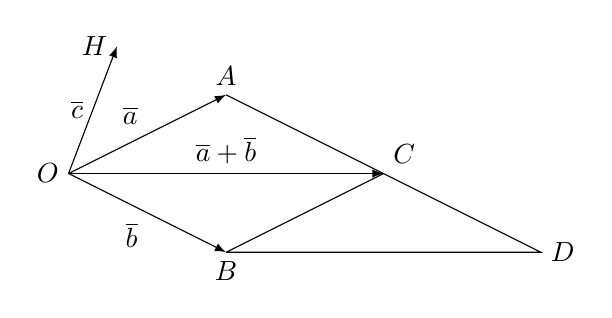
\begin{tikzpicture}[>=latex]
		\draw[->] (0, 0, 0) coordinate (O) node[left] {$O$}
				-- node[above left] {$\overline a$} (2, 1, 0) coordinate (A) node[above] {$A$};
		\draw[->] (O) -- node[below left] {$\overline b$} (2, -1, 0) coordinate (B) node[below] {$B$};
		\draw[->] (O) -- node[above] {$\overline a + \overline b$}
				(4, 0, 0) coordinate (C) node[above right] {$C$};
		\draw (C) -- (A)
			(B) -- (C) -- (6, -1, 0) coordinate (D) node[right] {$D$} -- (B);
		\draw[->] (O) -- node[left] {$\overline c$} (1, 2, 1) coordinate (H) node[left] {$H$};
		\end{tikzpicture}
		\end{flushright}
		\end{minipage}
	\end{enumerate}
	\end{proof}
\end{enumerate}
\section{Эллипс}
\index{Эллипс} \textbf{Эллипсом} называется геометрическое место точек~$M$ таких, что $MF_1 + MF_2 = 2a > F_1 F_2$, где $a$~--- константа.

Найдём уравнение эллипса.
Пусть $F_1 = (-c, 0)$, $F_2 = (c, 0)$, $M = (x, y)$.
\begin{equation*}
\sqrt{(x + c)^2 + y^2} + \sqrt{(x - c)^2 + y^2} = 2a \Rightarrow
2x^2 + 2y^2 + 2c^2 + 2\sqrt{(x^2 + y^2 + c^2)^2 - 4c^2 x^2} = 4a^2 \Rightarrow
\end{equation*}
\begin{equation*}
\Rightarrow (2a^2 - (x^2 + y^2 + c^2))^2 = (x^2 + y^2 + c^2)^2 - 4c^2 x^2 \Leftrightarrow
a^4 - a^2 x^2 - a^2 y^2 - a^2 c^2`+ c^2 x^2 = 0 \Leftrightarrow
(a^2 - c^2) x^2 + a^2 y^2 = a^2 (a^2 - c^2) \Leftrightarrow
\end{equation*}
\begin{equation*}
\left|\text{Пусть $b^2 = a^2 - c^2$}\right|
\Leftrightarrow b^2 x^2 + a^2 y^2 + a^2 b^2 \Leftrightarrow
\frac{x^2}{a^2} + \frac{y^2}{b^2} = 1
\end{equation*}

Найдём уравнение касательной, проходящей через точку~$(x_0, y_0)$ эллипса.
\begin{equation*}
y = \pm b\,\sqrt{1 - \frac{x^2}{a^2}} \Rightarrow
y' = \pm\frac{ab}{2\sqrt{a^2 - x^2}} \cdot \frac{-2x}{a^2} =
\mp\frac{bx}{a\sqrt{a^2 - x^2}} \;
\left|y = \pm b\,\sqrt{1 - \frac{x^2}{a^2}} \Leftrightarrow
\sqrt{a^2 - x^2} = \pm\frac{a}b\,y\right| =
-\frac{b^2 x}{a^2 y}
\end{equation*}
\begin{equation*}
y = y_0 - \frac{b^2 x_0}{a^2 y_0} (x - x_0) \Leftrightarrow
a^2 (y - y_0) y_0 = -b^2 (x - x_0) x_0 \Leftrightarrow
\frac{x x_0}{a^2} + \frac{y y_0}{b^2} - \left(\frac{x_0^2}{a^2} + \frac{y_0^2}{b^2} \right) = 0 \Leftrightarrow
\frac{x x_0}{a^2} + \frac{y y_0}{b^2} = 0
\end{equation*}
\section{Гипербола}
\begin{wrapfigure}[19]{r}{0pt}\noindent
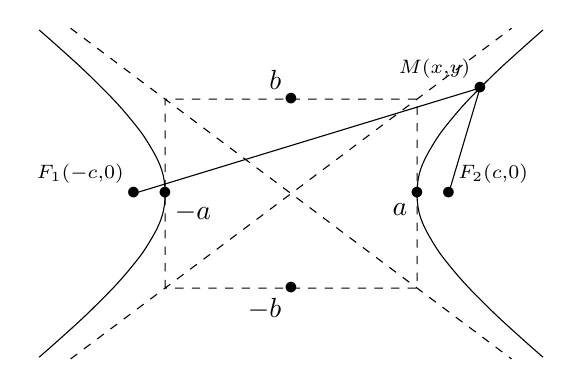
\begin{tikzpicture}[scale=0.4]
\drawaxis{-8}{8}{-5}{5};

% рисуем гиперболу x^2/16 - y^2/9 = 1
\draw (-5, 0) coordinate (F1) node {$\bullet$} node[above left] {$\scriptstyle F_1(-c, 0)$}
	(5, 0) coordinate (F2) node {$\bullet$} node[above right] {$\scriptstyle F_2(c, 0)$}
	(6, 3.3541) coordinate (M) node {$\bullet$} node [above left] {$\scriptstyle M(x, y)$}
	-- (F1) (M) -- (F2);
\def\painthyperbola[#1]{
\draw[#1] (4, 0)
	to[out=90, in=-121] (4.5, 1.5462)
	to[out=59, in=-129] (5, 9/4)
	to[out=51, in=-135] (6, 3.3541)
	to[out=45, in=-138] (7, 4.3084)
	to[out=42, in=-139] (8, 5.1962)
}
\painthyperbola[];
\painthyperbola[xscale=-1];
\painthyperbola[yscale=-1];
\painthyperbola[xscale=-1, yscale=-1];

% рисуем асимптоты
\draw[dashed] (-4, -3) rectangle (4, 3)
	(-7, 5.25) -- (7, -5.25)
	(-7, -5.25) -- (7, 5.25)
	(-4, 0) node {$\bullet$} node[below right] {$-a$}
	(4, 0) node {$\bullet$} node[below left] {$a$}
	(0, -3) node {$\bullet$} node[below left] {$-b$}
	(0, 3) node {$\bullet$} node[above left] {$b$};
\end{tikzpicture}
\end{wrapfigure}

\index{Гипербола} \textbf{Гиперболой} называется геометрическое место точек~$M$ таких, что $|MF_1 - MF_2| = 2a < F_1 F_2$, где $a$~--- константа, $F_1$ и $F_2$~--- фиксированные точки, называемые \textbf{фокусами гиперболы}.

Пусть $F_1 = (-c, 0)$, $F_2 = (c, 0)$, $M = (x, y)$.
Найдём уравнение гиперболы.
\begin{equation*}
\left|\sqrt{(x + c)^2 + y^2} - \sqrt{(x - c)^2 + y^2}\right| = 2a \Rightarrow
\end{equation*}
\begin{equation*}
\Rightarrow 2x^2 + 2y^2 + 2c^2 - 2\sqrt{(x^2 + y^2 + c^2)^2 - 4c^2 x^2} = 4a^2 \Rightarrow
\end{equation*}
\begin{equation*}
\Rightarrow (2a^2 - (x^2 + y^2 + c^2))^2 = (x^2 + y^2 + c^2)^2 - 4c^2 x^2 \Leftrightarrow
\end{equation*}
\begin{equation*}
\Leftrightarrow a^4 - a^2 x^2 - a^2 y^2 - a^2 c^2`+ c^2 x^2 = 0 \Leftrightarrow
\end{equation*}
\begin{equation*}
\Leftrightarrow (a^2 - c^2) x^2 + a^2 y^2 = a^2 (a^2 - c^2) \Leftrightarrow
\end{equation*}
\begin{equation*}
\left|\text{Пусть $b^2 = c^2 - a^2$}\right|
\Leftrightarrow -b^2 x^2 + a^2 y^2 = -a^2 b^2 \Leftrightarrow
\frac{x^2}{a^2} - \frac{y^2}{b^2} = 1
\end{equation*}

\subsection{Уравнение касательной}
Найдём уравнение касательной, проходящей через точку~$(x_0, y_0)$ гиперболы.
\begin{equation*}
y = \pm b\,\sqrt{\frac{x^2}{a^2} - 1} \Rightarrow
y' = \pm\frac{ab}{2\sqrt{x^2 - a^2}} \cdot \frac{2x}{a^2} =
\pm\frac{bx}{a\sqrt{x^2 - a^2}} \;
\left|y = \pm b\,\sqrt{\frac{x^2}{a^2} - 1} \Leftrightarrow
\sqrt{x^2 - a^2} = \pm\frac{a}b\,y\right| =
\frac{b^2 x}{a^2 y}
\end{equation*}
\begin{equation*}
y = y_0 + \frac{b^2 x_0}{a^2 y_0} (x - x_0) \Leftrightarrow
a^2 (y - y_0) y_0 = b^2 (x - x_0) x_0 \Leftrightarrow
\frac{x x_0}{a^2} - \frac{y y_0}{b^2} - \left(\frac{x_0^2}{a^2} - \frac{y_0^2}{b^2} \right) = 0 \Leftrightarrow
\frac{x x_0}{a^2} - \frac{y y_0}{b^2} = 0
\end{equation*}

\subsection{Асимптоты}
Докажем, что прямые~$y = \pm\frac{b}a\,x$~--- асимптоты гиперболы.
Пусть точка~$M(x, y)$ лежит на гиперболе, где $y > 0$, а точка~$N(x, Y)$~--- на прямой~$y = \frac{b}a\,x$.
Тогда
\begin{equation*}
MN = \frac{b}a \left(x - \sqrt{x^2 - a^2}\right) =
\frac{ab}{x + \sqrt{x^2 - a^2}} \Rightarrow
\lim_{x \to +\infty} MN =
\lim_{x \to +\infty} \frac{ab}{x + \sqrt{x^2 - a^2}} = 0
\end{equation*}

Рсстояние~$MN$ стремится к нулю при возрастании абсциссы, значит, $y = \frac{b}a\,x$~--- асимптота гиперболы.

Аналогично доказывается для случая~$y < 0$ и для прямой~$y = -\frac{b}a\,x$.
\section{Парабола}
\begin{wrapfigure}{r}{0pt}\noindent
\begin{tikzpicture}[scale=0.5]
\drawaxis{-3.5}{6}{-3}{7};

% рисуем параболу y^2 = 5x
\draw (-5/4, 0) coordinate (H)
	node {$\bullet$} node[below left] {$\scriptstyle (-\frac{p}2, 0)$}
	(H |- 0, \bottom_y) -- (H |- 0, \top_y)
	(5/4, 0) coordinate (F)
	node {$\bullet$} node[below] {$\scriptstyle F(\frac{p}2, 0)$}
	-- (5, 5) coordinate (M)
	node {$\bullet$} node[above left] {$\scriptstyle M(x, y)$}
	-| (H)
	(M -| H) rectangle +(10pt, 10pt);
\draw[rotate=-90] (-5.91608, 7) parabola bend (0, 0) (5.91608, 7);
\end{tikzpicture}
\end{wrapfigure}

\index{Парабола} \textbf{Параболой} называется геометрическое место точек~$M$ таких, что расстояния от~$M$ до некоторой прямой, называемой \textbf{директрисой}, и до некоторой точки, называемой \textbf{фокусом}, равны.

Пусть директриса задаётся уравнением $x = -\frac{p}2$, а фокус имеет координаты~$\left(\frac{p}2, 0\right)$.
Найдём уравнение параболы.
\begin{equation*}
\left(x + \frac{p}2\right)^2 = \left(x - \frac{p}2\right)^2 + y^2 \Leftrightarrow
y^2 = 2px
\end{equation*}

\subsection{Уравнение касательной}
Найдём уравнение касательной, проходящей через точку~$(x_0, y_0)$ параболы.
\begin{equation*}
y = \pm\sqrt{2px} \Rightarrow
y' = \pm\frac{p}{\sqrt{2px}} =
\pm\frac{\sqrt{2px}}{2x} =
\frac{y}{2x}
\end{equation*}
\begin{equation*}
y = y_0 + \frac{y_0}{2x_0} (x - x_0) \Leftrightarrow
2 x_0 (y - y_0) = y_0 (x - x_0) \Leftrightarrow
\end{equation*}
\begin{equation*}
\Leftrightarrow 2 x_0 y = y_0 (x + x_0) \Leftrightarrow
2 x_0 y_0 y = y_0^2 (x + x_0) \Leftrightarrow
2 y y_0 = 2p(x + x_0)
\end{equation*}
\section{Уравнения первой степени}
Уравнение вида~$Ax + By + Cz + D = 0$, где $x, y, z$~--- переменные, называется \textbf{уравнением первой степени}.

\begin{theorem}
\begin{itemize}
	\item Любое уравнение первой степени задаёт плоскость.
	\item Любая плоскость задаётся уравнением первой степени.
\end{itemize}
\end{theorem}
\begin{proof}
\begin{itemize}
	\item Пусть $(x_0, y_0, x_0)$~--- решение уравнения $Ax + By + Cz + D = 0$, $\overline m = (x - x_0, y - y_0, z_0)$, $\overline n = (A, B, C)$, тогда $A(x - x_0) + B(y - y_0) + C(z - z_0) = 0 \Leftrightarrow \overline n \perp \overline m$.
	Т.\,о., $\overline m$ независимо от значений $x, y, z$ всегда лежит в одной и той же плоскости.
	
	\item Пусть $(x_0, y_0, z_0)$~--- некоторая точка плоскости~$\pi$, вектор~$\overline n = (A, B, C) \perp \pi$, тогда $\forall (x, y, z) \in \pi \ A(x - x_0) + B(y - y_0) + C(z - z_0) = 0 \Leftrightarrow Ax + By + Cz - (Ax_0 + By_0 + Cz_0) = 0$.
\end{itemize}
\end{proof}

\index{Уравнения!плоскости} Т.\,о., уравнение
\begin{equation*}
Ax + By + Cz + D = 0
\end{equation*}
называется \textbf{общим уравнением плоскости}.
Если хотя бы один из коэффициентов равен нулю, то уравнение называется \textbf{неполным}.

\index{Нормаль} Вектор, перпендикулярный плоскости, называется \textbf{нормальным вектором} (\textbf{нормалью}) плоскости.

Пусть $(A, B, C)$~--- нормаль плоскости, $(x_0, 0, 0), (0, y_0, 0), (0, 0, z_0), (x_1, y_1, z_1), (x_2, y_2, z_2), (x_3, y_3, z_3)$~--- точки, лежащие на ней.

Тогда плоскость задаётся уравнением
\begin{equation*}
A(x - x_1) + B(y - y_1) + C(z - z_1) = 0
\end{equation*}

Также плоскость можно задать уравнением
\begin{equation*}
\begin{vmatrix}
x - x_1 & y - y_1 & z - z_1 \\
x_2 - x_1 & y_2 - y_1 & z_2 - z_1 \\
x_3 - x_1 & y_3 - y_1 & z_3 - z_1
\end{vmatrix} = 0
\end{equation*}

\textbf{Уравнением плоскости в отрезках} называется уравнение
\begin{equation*}
\frac{x}{x_0} + \frac{y}{y_0} + \frac{z}{z_0} = 1
\end{equation*}

\textbf{Нормальным} (\textbf{нормированным}) \textbf{уравнением плоскости} называется уравнение
\begin{equation*}
x \cos \alpha + y \cos \beta + z \cos \gamma - p = 0
\end{equation*}
где $\cos \alpha, \cos \beta, \cos \gamma$~--- направляющие косинусы вектора~$(A, B, C)$, $p$~--- расстояние от начала координат до плоскости.
\begin{proof}
Пусть $\overline n = (\cos \alpha, \cos \beta, \cos \gamma)$, $OM$~--- перпендикуляр, опущенный из начала координат~$O$ на плоскость, тогда $M = (p \cos \alpha, p \cos \beta, p \cos \gamma)$.
\begin{equation*}
(x - p \cos \alpha) \cos \alpha + (y - p \cos \beta) \cos \beta + (z - p \cos \gamma) \cos \gamma = 0 \Leftrightarrow
x \cos \alpha + y \cos \beta + z \cos \gamma - p = 0
\end{equation*}
\end{proof}

Пусть две плоскости заданы уравнениями $\alpha_1 \colon A_1 x + B_1 y + C_1 z + D_1 = 0$ и $\alpha_2 \colon A_2 x + B_2 y + C_2 z + D_2 = 0$, тогда:
\begin{itemize}
	\item $\displaystyle \alpha_1 = \alpha_2 \Leftrightarrow
	\frac{A_1}{A_2} = \frac{B_1}{B_2} = \frac{C_1}{C_2} = \frac{D_1}{D_2}$;
	\item $\displaystyle \alpha_1 \parallel \alpha_2 \Leftrightarrow
	\frac{A_1}{A_2} = \frac{B_1}{B_2} = \frac{C_1}{C_2}$;
	\item $\displaystyle \alpha_1 \perp \alpha_2 \Leftrightarrow
	A_1 A_2 + B_1 B_2 + C_1 C_2 = 0$;
	\item $\displaystyle \angle(\alpha_1, \alpha_2) = \arccos \frac{|A_1 A_2 + B_1 B_2 + C_1 C_2|}{\sqrt{A_1^2 + B_1^2 + C_1^2} \cdot \sqrt{A_2^2 + B_2^2 + C_2^2}}$.
\end{itemize}

Пусть задана плоскость $x \cos \alpha + y \cos \beta + z \cos \gamma - p = 0$ и точка~$M(x_0, y_0, z_0)$.

\index{Отклонение} \textbf{Отклонением точки от плоскости} называется расстояние между ними со знаком плюс, если начало координат и точка находятся с разных сторон плоскости, иначе со знаком минус, и равно $\delta = x_0 \cos \alpha + y_0 \cos \beta + z_0 \cos \gamma - p$.

Расстояние между точкой и плоскостью равно $|\delta|$.

\subsection{Уравнения, задающие прямую}
\index{Уравнения!прямой} \textbf{Общим уравнением прямой} называется
\begin{equation*}
\begin{cases}
A_1 x + B_1 y + C_1 z + D_1 = 0 \\
A_2 x + B_2 y + C_2 z + D_2 = 0
\end{cases}
\end{equation*}

Пусть $(a, b, c)$~--- направляющий вектор прямой, $(x_1, y_1, z_1), (x_2, y_2, z_2)$~--- точки, лежащие на ней.

\textbf{Каноническим уравнением прямой} называется уравнение
\begin{equation*}
\frac{x - x_1}a = \frac{y - y_1}b = \frac{z - z_1}c
\end{equation*}

Также прямую можно задать уравнением
\begin{equation*}
\frac{x - x_1}{x_2 - x_1} = \frac{y - y_1}{y_2 - y_1} = \frac{z - z_1}{z_2 - z_1}
\end{equation*}

\textbf{Параметрическим уравнением прямой} называется система
\begin{equation*}
\begin{cases}
x = x_1 + at \\
y = y_1 + bt \\
z = z_1 + ct
\end{cases}
\end{equation*}
\begin{proof}
Каноническое уравнение можно записать в виде $(x - x_1, y - y_1, z - z_1) = t \cdot (a,x b, c)$.
Записав его покоординатно, получим параметрическое уравнение.
\end{proof}
\section{Уравнения второй степени}
\label{sect:second_degree_equations_on_plane}
Уравнение вида $a_{11} x^2 + 2 a_{12} xy + a_{22} y^2 + 2 a_{13} x + 2 a_{23} y + a_{33} = 0$, где $x, y$~--- переменные, называется \textbf{уравнением второй степени}.
Одночлены $a_{11} x^2, 2 a_{12} xy, a_{22} y^2$ называются \textbf{старшими}, а остальные~--- \textbf{линейными}.

\textbf{Инвариантами} называются следующие определители:
\begin{enumerate}
	\item $I_1 = a_{11} + a_{22}$
	
	\item $I_2 =
	\begin{vmatrix}
	a_{11} & a_{12} \\
	a_{12} & a_{22}
	\end{vmatrix}$
	
	\item $I_3 =
	\begin{vmatrix}
	a_{11} & a_{12} & a_{13} \\
	a_{12} & a_{22} & a_{23} \\
	a_{13} & a_{23} & a_{33}
	\end{vmatrix}$
\end{enumerate}

Преобразуем кривую, задаваемую данным уравнением.
\begin{itemize}
	\item Применим параллельный перенос на вектор~$(a, b)$ и получим
	\begin{equation*}
	a_{11} (x + a)^2 + 2 a_{12} (x + a)(y + b) + a_{22} (y + b)^2 + 2 a_{13} (x + a) + 2 a_{23} (y + b) + a_{33} = 0 \Leftrightarrow
	\end{equation*}
	\begin{equation*}
	\Leftrightarrow a_{11} x^2 + 2 a_{12} xy + a_{22} y^2 +
	2 (a_{11} a + a_{12} b + a_{13}) x + 2 (a_{12} a + a_{22} b + a_{23}) y +
	a_{11} a^2 + 2 a_{12} ab + a_{22} b^2 + 2 a_{13} a + 2 a_{23} b + a_{33} = 0
	\end{equation*}
	
	\item Применим поворот на угол~$\alpha$ и получим
	\begin{equation*}
	a_{11} (x \cos \alpha + y \sin \alpha)^2 - 2 a_{12} (x \cos \alpha + y \sin \alpha) (x \sin \alpha - y \cos \alpha) + a_{22} (x \sin \alpha - y \cos \alpha)^2 + {}
	\end{equation*}
	\begin{equation*}
	{} + 2 a_{13} (x \cos \alpha + y \sin \alpha) - 2 a_{23} (x \sin \alpha - y \cos \alpha) + a_{33} = 0 \Leftrightarrow
	\end{equation*}
	\begin{equation*}
	\Leftrightarrow (a_{11} \cos^2 \alpha - a_{12} \sin 2\alpha + a_{22} \sin^2 \alpha) x^2 +
	(a_{11} \sin 2\alpha + 2 a_{12} \cos 2\alpha - a_{22} \sin 2\alpha) xy + {}
	\end{equation*}
	\begin{equation*}
	{} + (a_{11} \sin^2 \alpha + a_{12} \sin 2\alpha + a_{22} \cos^2 \alpha) y^2 +
	2 (a_{13} \cos \alpha - a_{23} \sin \alpha) x + 2 (a_{13} \sin \alpha + a_{23} \cos \alpha) y + a_{33} = 0
	\end{equation*}
\end{itemize}

В дальнейшем при преобразованиях новые коэффициенты в уравнении могут обозначаться $a_{11}', a_{12}', \ldots$ или же для удобства записи $a_{11}, a_{12}, \ldots$

\begin{theorem}
$I_1$, $I_2$, $I_3$ не меняются при параллельном переносе и поворотах.
\end{theorem}
\begin{proof}
\begin{itemize}
	\item Вычислим новые значения инвариантов после параллельного переноса:
	\begin{equation*}
	a_{11} + a_{22} = I_1
	\end{equation*}
	\begin{equation*}
	\begin{vmatrix}
	a_{11} & a_{12} \\
	a_{12} & a_{22}
	\end{vmatrix} = I_2
	\end{equation*}
	\begin{equation*}
	\begin{vmatrix}
	a_{11} & a_{12} & a_{11} a + a_{12} b + a_{13} \\
	a_{12} & a_{22} & a_{12} a + a_{22} b + a_{23} \\
	a_{11} a + a_{12} b + a_{13} & a_{12} a + a_{22} b + a_{23} & a_{11} a^2 + 2 a_{12} ab + a_{22} b^2 + 2 a_{13} a + 2 a_{23} b + a_{33}
	\end{vmatrix} =
	\end{equation*}
	\begin{equation*}
	= (a_{11} a + a_{12} b + a_{13}) (a_{12}^2 a + a_{12} a_{22} b + a_{12} a_{23} - a_{11} a_{22} a - a_{12} a_{22} b - a_{13} a_{22}) - {}
	\end{equation*}
	\begin{equation*}
	{} - (a_{12} a + a_{22} b + a_{23}) (a_{11} a_{12} a + a_{11} a_{22} b + a_{11} a_{23} - a_{11} a_{12} a - a_{12}^2 b - a_{12} a_{13}) + {}
	\end{equation*}
	\begin{equation*}
	{} + (a_{11} a^2 + 2 a_{12} ab + a_{22} b^2 + 2 a_{13} a + 2 a_{23} b + a_{33}) (a_{11} a_{22} - a_{12}^2) =
	\end{equation*}
	\begin{equation*}
	= a_{12} a_{13} a_{23} - a_{13}^2 a_{22} - a_{11} a_{23}^2 + a_{12} a_{13} a_{23} + a_{11} a_{22} a_{33} - a_{12}^2 a_{33} =
	\begin{vmatrix}
	a_{11} & a_{12} & a_{13} \\
	a_{12} & a_{22} & a_{23} \\
	a_{13} & a_{23} & a_{33}
	\end{vmatrix} = I_3
	\end{equation*}
	
	\item Вычислим новые значения инвариантов после поворота:
	\begin{equation*}
	a_{11} \cos^2 \alpha - a_{12} \sin 2\alpha + a_{22} \sin^2 \alpha +
	a_{11} \sin^2 \alpha + a_{12} \sin 2\alpha + a_{22} \cos^2 \alpha =
	a_{11} + a_{22} = I_1
	\end{equation*}
	\begin{equation*}
	\begin{vmatrix}
	a_{11} \cos^2 \alpha - a_{12} \sin 2\alpha + a_{22} \sin^2 \alpha & \frac12 a_{11} \sin 2\alpha + a_{12} \cos 2\alpha - \frac12 a_{22} \sin 2\alpha \\
	\frac12 a_{11} \sin 2\alpha + a_{12} \cos 2\alpha - \frac12 a_{22} \sin 2\alpha & a_{11} \sin^2 \alpha + a_{12} \sin 2\alpha + a_{22} \cos^2 \alpha
	\end{vmatrix} =
	\end{equation*}
	\begin{equation*}
	= (a_{11} \cos^2 \alpha - a_{12} \sin 2\alpha + a_{22} \sin^2 \alpha) (a_{11} \sin^2 \alpha + a_{12} \sin 2\alpha + a_{22} \cos^2 \alpha) - {}
	\end{equation*}
	\begin{equation*}
	{} - \left(\frac12 a_{11} \sin 2\alpha + a_{12} \cos^2 \alpha - a_{12} \sin^2 \alpha - \frac12 a_{22} \sin 2\alpha\right)^2 =
	\end{equation*}
	\begin{equation*}
	= \frac14 (a_{11}^2 - 4 a_{12}^2 + a_{22}^2 - a_{11}^2 - a_{22}^2 + 2 a_{11} a_{22} + 2 a_{12}^2) \sin^2 2\alpha +
	(a_{11} a_{22} - a_{12}^2) \cos^4 \alpha + (a_{11} a_{22} - a_{12}^2) \sin^4 \alpha + {}
	\end{equation*}
	\begin{equation*}
	{} + (a_{11} a_{12} - a_{12} a_{22} - a_{11} a_{12} + a_{12} a_{22}) \cos^2 \alpha \sin 2\alpha +
	(a_{12} a_{22} - a_{11} a_{12} + a_{11} a_{12} - a_{12} a_{22}) \sin^2 \alpha \sin 2\alpha =
	\end{equation*}
	\begin{equation*}
	= -\frac12 a_{12}^2 (\sin^2 2\alpha + 2 \cos^4 \alpha + 2 \sin^4 \alpha) +
	\frac12 a_{11} a_{22} (\sin^2 2\alpha + 2\cos^4 \alpha + 2\sin^4 \alpha) =
	a_{11} a_{22} - a_{12}^2 =
	\begin{vmatrix}
	a_{11} & a_{12} \\
	a_{12} & a_{22}
	\end{vmatrix} = I_2
	\end{equation*}
	\begin{equation*}
	\begin{vmatrix}
	a_{11} \cos^2 \alpha - a_{12} \sin 2\alpha + a_{22} \sin^2 \alpha & \frac12 a_{11} \sin 2\alpha + a_{12} \cos 2\alpha - \frac12 a_{22} \sin 2\alpha & a_{13} \cos \alpha - a_{23} \sin \alpha \\
	\frac12 a_{11} \sin 2\alpha + a_{12} \cos 2\alpha - \frac12 a_{22} \sin 2\alpha & a_{11} \sin^2 \alpha + a_{12} \sin 2\alpha + a_{22} \cos^2 \alpha & a_{13} \sin \alpha + a_{23} \cos \alpha \\
	a_{13} \cos \alpha - a_{23} \sin \alpha & a_{13} \sin \alpha + a_{23} \cos \alpha & a_{33}
	\end{vmatrix} =
	\end{equation*}
	\begin{equation*}
	= (a_{13} \cos \alpha - a_{23} \sin \alpha) \cdot
	\begin{vmatrix}
	\frac12 a_{11} \sin 2\alpha + a_{12} \cos^2 \alpha - a_{12} \sin^2 \alpha - \frac12 a_{22} \sin 2\alpha & a_{13} \cos \alpha - a_{23} \sin \alpha \\
	a_{11} \sin^2 \alpha + a_{12} \sin 2\alpha + a_{22} \cos^2 \alpha & a_{13} \sin \alpha + a_{23} \cos \alpha
	\end{vmatrix} - {}
	\end{equation*}
	\begin{equation*}
	{} - (a_{13} \sin \alpha + a_{23} \cos \alpha) \cdot
	\begin{vmatrix}
	a_{11} \cos^2 \alpha - a_{12} \sin 2\alpha + a_{22} \sin^2 \alpha & a_{13} \cos \alpha - a_{23} \sin \alpha \\
	\frac12 a_{11} \sin 2\alpha + a_{12} \cos^2 \alpha - a_{12} \sin^2 \alpha - \frac12 a_{22} \sin 2\alpha & a_{13} \sin \alpha + a_{23} \cos \alpha \\
	\end{vmatrix}
	+ a_{33} I_2 =
	\end{equation*}
	\begin{equation*}
	= \frac12 (a_{13} \cos \alpha - a_{23} \sin \alpha) \cdot
	((\cancel{a_{11} a_{13}} - \cancel{a_{12} a_{23}} - a_{22} a_{13} - \cancel{a_{11} a_{13}} + \cancel2 a_{12} a_{23}) \sin \alpha \sin 2\alpha + {}
	\end{equation*}
	\begin{equation*}
	{} + (a_{11} a_{23} + \cancel{a_{12} a_{13}} - \cancel{a_{22} a_{23}} - \cancel2 a_{12} a_{13} + \cancel{a_{22} a_{23}}) \cos \alpha \sin 2\alpha + {}
	\end{equation*}
	\begin{equation*}
	{} + 2(a_{12} a_{23} - a_{13} a_{22}) \cos^3 \alpha -
	2(a_{12} a_{13} - a_{11} a_{23}) \sin^3 \alpha) + {}
	\end{equation*}
	\begin{equation*}
	{} + \frac12 (a_{13} \sin \alpha + a_{23} \cos \alpha) \cdot
	((\cancel2 a_{12} a_{13} - \cancel{a_{22} a_{23}} - a_{11} a_{23} - \cancel{a_{12} a_{13}} + \cancel{a_{22} a_{23}}) \sin \alpha \sin 2\alpha + {}
	\end{equation*}
	\begin{equation*}
	{} + (\cancel{-a_{11} a_{13}} + \cancel2 a_{12} a_{23} + \cancel{a_{11} a_{13}} - \cancel{a_{12} a_{23}} - a_{22} a_{13}) \cos \alpha \sin 2\alpha - {}
	\end{equation*}
	\begin{equation*}
	{} - 2(a_{11} a_{23} - a_{12} a_{13}) \cos^3 \alpha -
	2(a_{22} a_{13} - a_{12} a_{23}) \sin^3 \alpha) + a_{33} I_2 =
	\end{equation*}
	\begin{equation*}
	= \frac14 (a_{12} a_{13} a_{23} - a_{13}^2 a_{22} - a_{11} a_{23}^2 + a_{12} a_{13} a_{23} - a_{11} a_{23}^2 + a_{12} a_{13} a_{23} + a_{12} a_{13} a_{23} - a_{13}^2 a_{22}) \sin^2 2\alpha + {}
	\end{equation*}
	\begin{equation*}
	{} + (a_{12} a_{13} a_{23} - a_{13}^2 a_{22} + a_{12} a_{13} a_{23} - a_{11} a_{23}^2) \cos^4 \alpha +
	(a_{12} a_{13} a_{23} - a_{11} a_{23}^2 + a_{12} a_{13} a_{23} - a_{13}^2 a_{22}) \sin^4 \alpha + {}
	\end{equation*}
	\begin{equation*}
	{} + \frac12 (a_{13} a_{22} a_{23} - a_{12} a_{23}^2 - a_{12} a_{13}^2 + a_{11} a_{13} a_{23} - a_{11} a_{13} a_{23} + a_{12} a_{13}^2 - a_{13} a_{22} a_{23} + a_{12} a_{23}^2) \sin^2 \alpha \sin 2\alpha + {}
	\end{equation*}
	\begin{equation*}
	{} + \frac12 (a_{11} a_{13} a_{23} - a_{12} a_{13}^2 - a_{12} a_{23}^2 + a_{13} a_{22} a_{23} + a_{12} a_{23}^2 - a_{13} a_{22} a_{23} - a_{11} a_{13} a_{23} - a_{12} a_{13}^2) \cos^2 \alpha \sin 2\alpha + a_{33} I_2 =
	\end{equation*}
	\begin{equation*}
	= (2a_{12} a_{13} a_{23} - a_{13}^2 a_{22} - a_{11} a_{23}^2) \left(\sin^4 \alpha + \frac12 \sin^2 2\alpha + \cos^4 \alpha\right) + a_{33} I_2 =
	\end{equation*}
	\begin{equation*}
	= a_{13} (a_{12} a_{23} - a_{13} a_{22}) + a_{23} (a_{12} a_{13} - a_{11} a_{23}) + a_{33} I_2 =
	\end{equation*}
	\begin{equation*}
	= a_{13} \cdot
	\begin{vmatrix}
	a_{12} & a_{13} \\
	a_{22} & a_{23}
	\end{vmatrix} -
	a_{23} \cdot
	\begin{vmatrix}
	a_{11} & a_{13} \\
	a_{12} & a_{23}
	\end{vmatrix} +
	a_{33} \cdot
	\begin{vmatrix}
	a_{11} & a_{12} \\
	a_{12} & a_{22}
	\end{vmatrix} =
	\begin{vmatrix}
	a_{11} & a_{12} & a_{13} \\
	a_{12} & a_{22} & a_{23} \\
	a_{13} & a_{23} & a_{33}
	\end{vmatrix} = I_3
	\end{equation*}
\end{itemize}
\end{proof}

Если $I_2 \neq 0$, то $\exists! (x_0, y_0) \colon
\begin{cases}
a_{11} x_0 + a_{12} y_0 + a_{13} = 0 \\
a_{12} x_0 + a_{22} y_0 + a_{23} = 0
\end{cases}$ и систему координат можно перенести на вектор~$(x_0, y_0)$, получив уравнение
\begin{equation*}
a_{11} x^2 + 2 a_{12} xy + a_{22} y^2 + a_{33} = 0
\end{equation*}

В таком случае кривая называется \textbf{центральной}, а точка~$(x_0, y_0)$~--- её \textbf{центром}.

Найдём такой угол~$\varphi$, что $a_{12}' = 0$ при повороте на этот угол.
\begin{enumerate}
	\item Пусть $a_{11} \neq a_{22}$, тогда
	\begin{equation*}
	a_{11} \sin 2\varphi + 2 a_{12} \cos 2\varphi - a_{22} \sin 2\varphi = 0 \Leftrightarrow
	2 a_{12} \cos 2\varphi = (a_{22} - a_{11}) \sin 2\varphi \Leftrightarrow
	\varphi = \frac12 \arctg \frac{2 a_{12}}{a_{22} - a_{11}}
	\end{equation*}
	
	\item Пусть $a_{11} = a_{22}$, тогда $2 a_{12} \cos 2\varphi = 0 \Leftrightarrow
	\varphi = \frac\pi4$.
\end{enumerate}
                                                              
Т.\,о., далее можно ограничиться рассмотрением уравнений вида $a_{11} x^2 + a_{22} y^2 + 2 a_{13} x + 2 a_{23} y + a_{33} = 0$.
\begin{enumerate}
	\item Пусть $I_2 < 0$, тогда после параллельного переноса получим уравнение
	\begin{equation*}
	a_{11} x^2 + a_{22} y^2 + a_{33} = 0 \Leftrightarrow
	\frac{x^2}{a_{22}} + \frac{y^2}{a_{11}} = -\frac{a_{33}}{a_{11} a_{22}}
	\end{equation*}
	а также $a_{11} a_{22} = I_2 < 0$.
	\begin{itemize}
		\item Если $a_{33} \neq 0$, то получим гиперболу:
		$\displaystyle \frac{x^2}{a^2} - \frac{y^2}{b^2} = 1$
		\item Если $a_{33} = 0$, то получим две прямые, проходящие через~$(0, 0)$:
		$\displaystyle \frac{x^2}{a^2} - \frac{y^2}{b^2} = 0 \Leftrightarrow
		y = \pm\frac{b}a\,x$
	\end{itemize}
	
	\item Пусть $I_2 = 0$, тогда $a_{11} a_{22} = 0$.
	Т.\,к. уравнение второго порядка, то $a_{11} = 0 \lAnd a_{22} > 0$.
	Получим
	\begin{equation*}
	a_{22} y^2 + 2 a_{13} x + 2 a_{23} y + a_{33} = 0 \Leftrightarrow
	a_{22} \left(y + \frac{a_{23}}{a_{22}}\right)^2 + 2 a_{13} x + a_{33} - \frac{a_{23}^2}{a_{22}} = 0 \Rightarrow
	a_{22} y^2 + 2 a_{13} x + a_{33} = 0
	\end{equation*}
	\begin{itemize}
		\item Пусть $a_{13} = 0$, тогда $a_{22} y^2 + a_{33} = 0$.
		\begin{itemize}
			\item Если $a_{22} a_{33} \leqslant 0$, то получим две параллельные прямые:
			$\displaystyle \frac{y^2}{b^2} = 1 \Leftrightarrow
			y = \pm b$
			\item Если $a_{22} a_{33} > 0$, то получим пустое множество:
			$\displaystyle \frac{y^2}{b^2} = -1$
		\end{itemize}
		
		\item Пусть $a_{13} \neq 0$, тогда получим параболу
		\begin{equation*}
		a_{22} y^2 + 2 a_{13} x + a_{33} = 0 \Leftrightarrow
		y^2 + \frac{2 a_{13}}{a_{22}} \left(x + \frac{a_{33}}{2 a_{13}}\right) = 0 \Rightarrow
		y^2 = 2px
		\end{equation*}
	\end{itemize}
	
	\item Пусть $I_2 > 0$, тогда после параллельного переноса получим уравнение $a_{11} x^2 + a_{22} y^2 + a_{33} = 0$, а также $a_{11} a_{22} = I_2 > 0$.
	\begin{itemize}
		\item Если $a_{11} a_{33} \leqslant 0$, то получим эллипс:
		$\displaystyle \frac{x^2}{a^2} + \frac{y^2}{b^2} = 1$
		\item Если $a_{11} a_{33} > 0$, то получим пустое множество:
		$\displaystyle \frac{x^2}{a^2} + \frac{y^2}{b^2} = -1$
	\end{itemize}
\end{enumerate}

\begin{theorem}
Для канонической формы кривой второго порядка $a_{11}$ и $a_{22}$~--- корни характеристического многочлена $I_2$.
\end{theorem}
\chapter{Стереометрия}
\section{Векторы}
\index{Векторы!компланарные} Векторы называются \textbf{компланарными}, если они лежат в одной плоскости.

Некомпланарные векторы $\overline a, \overline b, \overline c$, начала которых находятся в одной точке, называются \textbf{правой тройкой~$(\overline a, \overline b, \overline c)$}, если с конца~$\overline c$ кратчайший поворот от~$\overline a$ к~$\overline b$ виден против часовой стрелки при условии, иначе~--- \textbf{левой тройкой~$(\overline a, \overline b, \overline c)$}.
Также говорят о \textbf{левой} или \textbf{правой ориентации тройки}.

\subsection{Векторное произведение}
\index{Произведение!векторное} Векторным произведением векторов $\overline a$ и $\overline b$ называется вектор~$\overline c$ такой, что:
\begin{itemize}
	\item $|\overline c| = |\overline a| \cdot |\overline b| \cdot \sin \angle(\overline a, \overline b)$
	\item $\overline c \perp \overline a \lAnd \overline c \perp \overline b$
	\item $(\overline a, \overline b, \overline c)$~--- правая тройка
\end{itemize}
и обозначается $[\overline a \cdot \overline b]$ или $[\overline a\,\overline b]$.

Свойства векторного произведения:
\begin{enumerate}
	\item $[\overline a\,\overline a] = \overline 0$
	\begin{proof}
	\begin{equation*}
	\angle(\overline a, \overline a) = 0 \Rightarrow
	|[\overline a\,\overline a]| = |\overline a|^2 \cdot \sin \angle(\overline a, \overline a) = 0 \Rightarrow
	[\overline a\,\overline a] = \overline 0
	\end{equation*}
	\end{proof}
	
	\item $[\overline a\,\overline b] = -[\overline b\,\overline a]$
	\begin{proof}
	Достаточно заметить, что тройки $(\overline a, \overline b, \overline c)$ и $(\overline b, \overline a, \overline c)$ имеют разную ориентацию.
	\end{proof}
	
	\item $\forall \alpha \in \mathbb R \ [(\alpha \overline a)\,\overline b] = \alpha [\overline a\,\overline b]$
	\begin{proof}
	\begin{enumerate}
		\item Пусть $\alpha < 0$, тогда $[(\alpha \overline a)\,\overline b] = -|\alpha| [\overline a\,\overline b] = \alpha [\overline a\,\overline b]$.
		\item Пусть $\alpha \geqslant 0$, тогда $[(\alpha \overline a)\,\overline b] = |\alpha| [\overline a\,\overline b] = \alpha [\overline a\,\overline b]$.
	\end{enumerate}
	\end{proof}
	
	\item $[(\overline a + \overline b)\,\overline c] = [\overline a\,\overline c] + [\overline b\,\overline c]$
	\begin{proof}
	\begin{enumerate}
		\item Пусть $\overline a, \overline b, \overline c$ лежат в плоскости~$\pi$.
		Введём векторы $\overline e \colon \overline e \in \pi \lAnd \overline e \perp \overline c$ и $\overline g$ такой, что:
		\begin{itemize}
			\item $[\overline a\,\overline c] = |\overline a| \cdot |\overline c| \cdot \sin \angle(\overline a, \overline c) \cdot \overline g$
			\item $[\overline b\,\overline c] = |\overline b| \cdot |\overline c| \cdot \sin \angle(\overline b, \overline c) \cdot \overline g$
		\end{itemize}
		
		Тогда
		\begin{equation*}
		[\overline a\,\overline c] = 
		|\overline a| \cdot |\overline c| \cdot \cos \angle(\overline a, \overline e) \cdot \overline g =
		\pr_{\overline e} \overline a \cdot |\overline c| \cdot \overline g
		\end{equation*}
		\begin{equation*}
		[\overline b\,\overline c] = 
		|\overline b| \cdot |\overline c| \cdot \cos \angle(\overline b, \overline e) \cdot \overline g =
		\pr_{\overline e} \overline a \cdot |\overline c| \cdot \overline g
		\end{equation*}
		\begin{equation*}
		[(\overline a + \overline b)\,\overline c] =
		\pr_{\overline e} (\overline a + \overline b) \cdot |\overline c| \cdot \overline g =
		\pr_{\overline e} \overline a \cdot |\overline c| \cdot \overline g +
		\pr_{\overline e} \overline b \cdot |\overline c| \cdot \overline g =
		[\overline a\,\overline c] + [\overline b\,\overline c]
		\end{equation*}
		
		\item Пусть $\overline a, \overline b, \overline c$ некомпланарны, тогда $[(\overline a + \overline b)\,\overline c], [\overline a\,\overline c], [\overline b\,\overline c] \perp \overline c \Rightarrow
		[(\overline a + \overline b)\,\overline c], [\overline a\,\overline c], [\overline b\,\overline c]$ компланарны $\Rightarrow$
		$\alpha [(\overline a + \overline b)\,\overline c] \opbr=
		\beta [\overline a\,\overline c] \opbr+ \gamma [\overline b\,\overline c]$.
		
		\begin{minipage}[t]{95mm}\noindent
		Докажем, что $\alpha = \beta$.
		\begin{itemize}
			\item $\alpha [(\overline a + \overline b)\,\overline c] =
			\beta [\overline a\,\overline c] + \gamma [\overline b\,\overline c] \Rightarrow
			\alpha (\overline a + \overline b)\,\overline c\,\overline b =
			\beta \overline a\,\overline c\,\overline b$
			
			\item Пусть $V_1$ и $V_2$~--- объёмы параллелепипедов, построенных на $OA$, $OB$, $OH$ и $OC$, $OB$, $OH$ соответственно, тогда $S(OACB) = S(OCDB) \opbr\Rightarrow
			V_1 = V_2 \opbr\Rightarrow
			\overline a\,\overline b\,\overline c = (\overline a + \overline b)\,\overline b\,\overline c \opbr\Rightarrow
			\overline a\,\overline c\,\overline b = (\overline a + \overline b)\,\overline c\,\overline b$
		\end{itemize}
		
		Отсюда $\alpha = \beta$.
		Аналогично $\alpha = \gamma$.
		\end{minipage}
		\hfill
		\begin{minipage}[t]{71mm}\noindent
		\begin{flushright}
		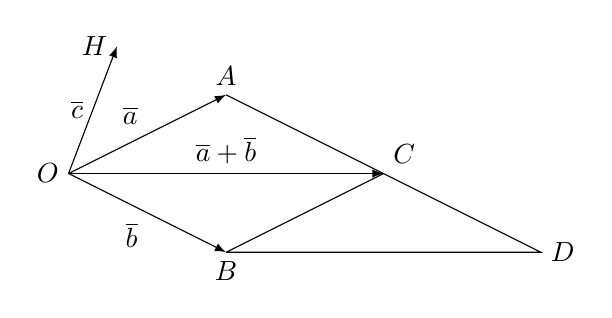
\begin{tikzpicture}[>=latex]
		\draw[->] (0, 0, 0) coordinate (O) node[left] {$O$}
				-- node[above left] {$\overline a$} (2, 1, 0) coordinate (A) node[above] {$A$};
		\draw[->] (O) -- node[below left] {$\overline b$} (2, -1, 0) coordinate (B) node[below] {$B$};
		\draw[->] (O) -- node[above] {$\overline a + \overline b$}
				(4, 0, 0) coordinate (C) node[above right] {$C$};
		\draw (C) -- (A)
			(B) -- (C) -- (6, -1, 0) coordinate (D) node[right] {$D$} -- (B);
		\draw[->] (O) -- node[left] {$\overline c$} (1, 2, 1) coordinate (H) node[left] {$H$};
		\end{tikzpicture}
		\end{flushright}
		\end{minipage}
	\end{enumerate}
	\end{proof}
\end{enumerate}
\section{Уравнения первой степени}
Уравнение вида~$Ax + By + Cz + D = 0$, где $x, y, z$~--- переменные, называется \textbf{уравнением первой степени}.

\begin{theorem}
\begin{itemize}
	\item Любое уравнение первой степени задаёт плоскость.
	\item Любая плоскость задаётся уравнением первой степени.
\end{itemize}
\end{theorem}
\begin{proof}
\begin{itemize}
	\item Пусть $(x_0, y_0, x_0)$~--- решение уравнения $Ax + By + Cz + D = 0$, $\overline m = (x - x_0, y - y_0, z_0)$, $\overline n = (A, B, C)$, тогда $A(x - x_0) + B(y - y_0) + C(z - z_0) = 0 \Leftrightarrow \overline n \perp \overline m$.
	Т.\,о., $\overline m$ независимо от значений $x, y, z$ всегда лежит в одной и той же плоскости.
	
	\item Пусть $(x_0, y_0, z_0)$~--- некоторая точка плоскости~$\pi$, вектор~$\overline n = (A, B, C) \perp \pi$, тогда $\forall (x, y, z) \in \pi \ A(x - x_0) + B(y - y_0) + C(z - z_0) = 0 \Leftrightarrow Ax + By + Cz - (Ax_0 + By_0 + Cz_0) = 0$.
\end{itemize}
\end{proof}

\index{Уравнения!плоскости} Т.\,о., уравнение
\begin{equation*}
Ax + By + Cz + D = 0
\end{equation*}
называется \textbf{общим уравнением плоскости}.
Если хотя бы один из коэффициентов равен нулю, то уравнение называется \textbf{неполным}.

\index{Нормаль} Вектор, перпендикулярный плоскости, называется \textbf{нормальным вектором} (\textbf{нормалью}) плоскости.

Пусть $(A, B, C)$~--- нормаль плоскости, $(x_0, 0, 0), (0, y_0, 0), (0, 0, z_0), (x_1, y_1, z_1), (x_2, y_2, z_2), (x_3, y_3, z_3)$~--- точки, лежащие на ней.

Тогда плоскость задаётся уравнением
\begin{equation*}
A(x - x_1) + B(y - y_1) + C(z - z_1) = 0
\end{equation*}

Также плоскость можно задать уравнением
\begin{equation*}
\begin{vmatrix}
x - x_1 & y - y_1 & z - z_1 \\
x_2 - x_1 & y_2 - y_1 & z_2 - z_1 \\
x_3 - x_1 & y_3 - y_1 & z_3 - z_1
\end{vmatrix} = 0
\end{equation*}

\textbf{Уравнением плоскости в отрезках} называется уравнение
\begin{equation*}
\frac{x}{x_0} + \frac{y}{y_0} + \frac{z}{z_0} = 1
\end{equation*}

\textbf{Нормальным} (\textbf{нормированным}) \textbf{уравнением плоскости} называется уравнение
\begin{equation*}
x \cos \alpha + y \cos \beta + z \cos \gamma - p = 0
\end{equation*}
где $\cos \alpha, \cos \beta, \cos \gamma$~--- направляющие косинусы вектора~$(A, B, C)$, $p$~--- расстояние от начала координат до плоскости.
\begin{proof}
Пусть $\overline n = (\cos \alpha, \cos \beta, \cos \gamma)$, $OM$~--- перпендикуляр, опущенный из начала координат~$O$ на плоскость, тогда $M = (p \cos \alpha, p \cos \beta, p \cos \gamma)$.
\begin{equation*}
(x - p \cos \alpha) \cos \alpha + (y - p \cos \beta) \cos \beta + (z - p \cos \gamma) \cos \gamma = 0 \Leftrightarrow
x \cos \alpha + y \cos \beta + z \cos \gamma - p = 0
\end{equation*}
\end{proof}

Пусть две плоскости заданы уравнениями $\alpha_1 \colon A_1 x + B_1 y + C_1 z + D_1 = 0$ и $\alpha_2 \colon A_2 x + B_2 y + C_2 z + D_2 = 0$, тогда:
\begin{itemize}
	\item $\displaystyle \alpha_1 = \alpha_2 \Leftrightarrow
	\frac{A_1}{A_2} = \frac{B_1}{B_2} = \frac{C_1}{C_2} = \frac{D_1}{D_2}$;
	\item $\displaystyle \alpha_1 \parallel \alpha_2 \Leftrightarrow
	\frac{A_1}{A_2} = \frac{B_1}{B_2} = \frac{C_1}{C_2}$;
	\item $\displaystyle \alpha_1 \perp \alpha_2 \Leftrightarrow
	A_1 A_2 + B_1 B_2 + C_1 C_2 = 0$;
	\item $\displaystyle \angle(\alpha_1, \alpha_2) = \arccos \frac{|A_1 A_2 + B_1 B_2 + C_1 C_2|}{\sqrt{A_1^2 + B_1^2 + C_1^2} \cdot \sqrt{A_2^2 + B_2^2 + C_2^2}}$.
\end{itemize}

Пусть задана плоскость $x \cos \alpha + y \cos \beta + z \cos \gamma - p = 0$ и точка~$M(x_0, y_0, z_0)$.

\index{Отклонение} \textbf{Отклонением точки от плоскости} называется расстояние между ними со знаком плюс, если начало координат и точка находятся с разных сторон плоскости, иначе со знаком минус, и равно $\delta = x_0 \cos \alpha + y_0 \cos \beta + z_0 \cos \gamma - p$.

Расстояние между точкой и плоскостью равно $|\delta|$.

\subsection{Уравнения, задающие прямую}
\index{Уравнения!прямой} \textbf{Общим уравнением прямой} называется
\begin{equation*}
\begin{cases}
A_1 x + B_1 y + C_1 z + D_1 = 0 \\
A_2 x + B_2 y + C_2 z + D_2 = 0
\end{cases}
\end{equation*}

Пусть $(a, b, c)$~--- направляющий вектор прямой, $(x_1, y_1, z_1), (x_2, y_2, z_2)$~--- точки, лежащие на ней.

\textbf{Каноническим уравнением прямой} называется уравнение
\begin{equation*}
\frac{x - x_1}a = \frac{y - y_1}b = \frac{z - z_1}c
\end{equation*}

Также прямую можно задать уравнением
\begin{equation*}
\frac{x - x_1}{x_2 - x_1} = \frac{y - y_1}{y_2 - y_1} = \frac{z - z_1}{z_2 - z_1}
\end{equation*}

\textbf{Параметрическим уравнением прямой} называется система
\begin{equation*}
\begin{cases}
x = x_1 + at \\
y = y_1 + bt \\
z = z_1 + ct
\end{cases}
\end{equation*}
\begin{proof}
Каноническое уравнение можно записать в виде $(x - x_1, y - y_1, z - z_1) = t \cdot (a,x b, c)$.
Записав его покоординатно, получим параметрическое уравнение.
\end{proof}
\section{Уравнения второго порядка}
Уравнение вида $a_{11} x^2 + a_{22} y^2 + a_{33} z^2 + 2 a_{12} xy + 2 a_{13} xz + 2 a_{23} yz + 2 a_{14} x + 2 a_{24} y + 2 a_{34} z + a_{44} = 0$, где $x, y, z$~--- переменные, называется \textbf{уравнением второй степени}.

\textbf{Инвариантами} называются следующие определители:
\begin{enumerate}
	\item $I_1 = a_{11} + a_{22} + a_{33}$
	
	\item $I_2 =
	\begin{vmatrix}
	a_{11} & a_{12} \\
	a_{12} & a_{22}
	\end{vmatrix} +
	\begin{vmatrix}
	a_{11} & a_{13} \\
	a_{13} & a_{33}
	\end{vmatrix} +
	\begin{vmatrix}
	a_{22} & a_{23} \\
	a_{23} & a_{33}
	\end{vmatrix}$
	
	\item $I_3 =
	\begin{vmatrix}
	a_{11} & a_{12} & a_{13} \\
	a_{12} & a_{22} & a_{23} \\
	a_{13} & a_{23} & a_{33}
	\end{vmatrix}$
	
	\item $I_4 =
	\begin{vmatrix}
	a_{11} & a_{12} & a_{13} & a_{14} \\
	a_{12} & a_{22} & a_{23} & a_{24} \\
	a_{13} & a_{23} & a_{33} & a_{34} \\
	a_{14} & a_{24} & a_{34} & a_{44}
	\end{vmatrix}$
\end{enumerate}

Применив к поверхности, задаваемой данным уравнением, параллельный перенос на вектор~$(a, b, c)$, получим
\begin{equation*}
a_{11} (x + a)^2 + a_{22} (y + b)^2 + a_{33} (z + c)^2 + 2 a_{12} (x + a)(y + b) + 2 a_{13} (x + a)(z + c) + 2 a_{23} (y + b)(z + c) + {}
\end{equation*}
\begin{equation*}
{} + 2 a_{14} (x + a) + 2 a_{24} (y + b) + 2 a_{34} (z + c) + a_{44} = 0 \Leftrightarrow
\end{equation*}
\begin{equation*}
\Leftrightarrow a_{11} x^2 + a_{22} y^2 + a_{33} z^2 + 2 a_{12} xy + 2 a_{13} xz + 2 a_{23} yz + {}
\end{equation*}
\begin{equation*}
{} + 2 (a_{11} a + a_{12} b + a_{13} c + a_{14}) x + 2 (a_{12} a + a_{22} b + a_{23} c + a_{24}) y + 2 (a_{13} a + a_{23} b + a_{33} c + a_{34}) z + {}
\end{equation*}
\begin{equation*}
{} + a_{11} a^2 + a_{22} b^2 + a_{33} c^2 + 2 a_{12} ab + 2 a_{13} ac + 2 a_{23} bc + 2 a_{14} a + 2 a_{24} b + 2 a_{34} c + a_{44} = 0
\end{equation*}

В дальнейшем при преобразованиях новые коэффициенты в уравнении могут обозначаться $a_{11}', a_{12}', \ldots$ или же для удобства записи $a_{11}, a_{12}, \ldots$

\begin{theorem}
$I_1$, $I_2$, $I_3$, $I_4$ не меняются при параллельном переносе и поворотах.
\end{theorem}

Если $I_3 \neq 0$, то $\exists! (x_0, y_0, z_0) \colon
\begin{cases}
a_{11} x_0 + a_{12} y_0 + a_{13} z_0 + a_{14} = 0 \\
a_{12} x_0 + a_{22} y_0 + a_{23} z_0 + a_{24} = 0 \\
a_{13} x_0 + a_{23} y_0 + a_{33} z_0 + a_{34} = 0 
\end{cases}$ и систему координат можно перенести на вектор~$(x_0, y_0, z_0)$, получив уравнение
\begin{equation*}
a_{11} x^2 + a_{22} y^2 + a_{33} z^2 + 2 a_{12} xy + 2 a_{13} xz + 2 a_{23} yz + a_{44} = 0
\end{equation*}

В таком случае поверхность называется \textbf{центральной}, а точка~$(x_0, y_0, z_0)$~--- её \textbf{центром}.

Найдём такой поворот, при котором $a_{13}' = a_{23}' = 0$.
Для этого введём функцию
\begin{equation*}
F(x, y, z) = a_{11} x^2 + a_{22} y^2 + a_{33} z^2 + 2 a_{12} xy + 2 a_{13} xz + 2 a_{23} yz, \
D(F) = \{ (x, y, z) \mid x^2 + y^2 + z^2 = 1 \}
\end{equation*}
и найдём точку $P \colon F(P) = \max F(x, y, z)$.

Теперь осуществим такой поворот, чтобы $Oz' = OP$, и рассмотрим плоскость $Ox'z'$.
В этой плоскости
\begin{equation*}
F(x, z) =
F(\sin \Theta, \cos \Theta) =
F(\Theta) =
a_{11} \sin^2 \Theta + a_{33} \cos^2 \Theta + 2 a_{13} \sin \Theta \cos \Theta =
\end{equation*}
\begin{equation*}
= \frac{a_{11}}2 (1 - \cos 2\Theta) + \frac{a_{33}}2 (1 + \cos 2\Theta) + a_{13} \sin 2\Theta =
a_{13} \sin 2\Theta - \frac{a_{11} - a_{33}}2\,\cos 2\Theta + \frac{a_{11} + a_{33}}2
\end{equation*}
\begin{equation*}
F'(\Theta) = 2 a_{13} \cos 2\Theta + (a_{11} - a_{33}) \sin 2\Theta
\end{equation*}

Тогда
\begin{equation*}
P = \max F \Rightarrow
F'(0) = 0 \Rightarrow
a_{13} = 0
\end{equation*}

Аналогично рассматривая плоскость, получим $a_{23} = 0$.
Затем применим поворот, описанный в разделе~\ref{sect:second_degree_equations_on_plane}, и получим $a_{12} = 0$.

Т.\,о., далее можно ограничиться рассмотрением уравнений вида $a_{11} x^2 + a_{22} y^2 + a_{33} z^2 + 2 a_{14} x + 2 a_{24} y + 2 a_{34} z \opbr+ a_{44} = 0$.
\begin{enumerate}
	\item Пусть $I_3 \neq 0$, тогда, найдя корни $\lambda_1, \lambda_2, \lambda_3$ характеристического многочлена, получим уравнение
	\begin{equation*}
	\lambda_1 x^2 + \lambda_2 y^2 + \lambda_3 z^2 + \frac{I_4}{I_3} = 0
	\end{equation*}
	\begin{enumerate}
		\item Пусть $I_4 \neq 0$, тогда получим
		\begin{equation*}
		\frac{x^2}{-\frac{I_4}{\lambda_1 I_3}} + \frac{y^2}{-\frac{I_4}{\lambda_2 I_3}} + \frac{z^2}{-\frac{I_4}{\lambda_3 I_3}} = 1
		\end{equation*}
		
		В зависимости от знаков коэффициентов получим
		\begin{itemize}
			\item Эллипсоид:
			$\displaystyle \frac{x^2}{a^2} + \frac{y^2}{b^2} + \frac{z^2}{c^2} = 1$
			\item Пустое множество:
			$\displaystyle \frac{x^2}{a^2} + \frac{y^2}{b^2} + \frac{z^2}{c^2} = -1$
			\item Однополостный гиперболоид:
			$\displaystyle \frac{x^2}{a^2} + \frac{y^2}{b^2} - \frac{z^2}{c^2} = 1 \Leftrightarrow
			\frac{x^2}{a^2} + \frac{y^2}{b^2} = \frac{z^2}{c^2} + 1$
			\item Двуполостный гиперболоид:
			$\displaystyle \frac{x^2}{a^2} + \frac{y^2}{b^2} - \frac{z^2}{c^2} = -1 \Leftrightarrow
			\frac{x^2}{a^2} + \frac{y^2}{b^2} = \frac{z^2}{c^2} - 1$
		\end{itemize}
		
		\item Пусть $I_4 = 0$, тогда получим
		\begin{equation*}
		\frac{x^2}{\frac1{\lambda_1}} + \frac{y^2}{\frac1{\lambda_2}} + \frac{z^2}{\frac1{\lambda_3}} = 0
		\end{equation*}
		
		В зависимости от знаков коэффициентов получим
		\begin{itemize}
			\item Вырожденный конус (точка~$(0, 0, 0)$):
			$\displaystyle \frac{x^2}{a^2} + \frac{y^2}{b^2} + \frac{z^2}{c^2} = 0$
			\item Конус:
			$\displaystyle \frac{x^2}{a^2} + \frac{y^2}{b^2} - \frac{z^2}{c^2} = 0$
		\end{itemize}
	\end{enumerate}
	
	\item Пусть $I_3 = 0$, тогда
	\begin{equation*}
	\begin{vmatrix}
	a_{11} & 0 & 0 \\
	0 & a_{22} & 0 \\
	0 & 0 & a_{33}
	\end{vmatrix} = 0 \Leftrightarrow
	a_{11} a_{22} a_{33} = 0
	\end{equation*}
	\begin{enumerate}
		\item Пусть $a_{11}, a_{22} \neq 0$, $a_{33} = 0$, тогда
		\begin{equation*}
		a_{11} x^2 + a_{22} y^2 + 2 a_{14} x + 2 a_{24} y + 2 a_{34} z + a_{44} = 0 \Leftrightarrow
		\end{equation*}
		\begin{equation*}
		\Leftrightarrow a_{11} \left(x + \frac{a_{14}}{a_{11}}\right)^2 + a_{22} \left(y + \frac{a_{24}}{a_{22}}\right)^2 + 2 a_{34} z + a_{44} - \frac{a_{14}^2}{a_{11}} - \frac{a_{24}^2}{a_{22}} = 0 \Rightarrow
		\end{equation*}
		\begin{equation*}
		\Rightarrow a_{11} x^2 + a_{22} y^2 + 2 p z + q = 0
		\end{equation*}
		\begin{itemize}
			\item Пусть $p = q = 0$, тогда $a_{11} x^2 + a_{22} y^2 = 0$.
			\begin{itemize}
				\item Если $a_{11} a_{22} < 0$, то получим две пересекающиеся плоскости:
				$\displaystyle \frac{x^2}{a^2} - \frac{y^2}{b^2} = 0 \Leftrightarrow
				y = \pm\frac{b}a\,x$
				\item Если $a_{11} a_{22} > 0$, то получим прямую:
				$\displaystyle \frac{x^2}{a^2} + \frac{y^2}{b^2} = 0 \Leftrightarrow
				x = y = 0$
			\end{itemize}
			
			\item Пусть $p = 0$, $q \neq 0$, тогда
			\begin{equation*}
			a_{11} x^2 + a_{22} y^2 + q = 0 \Leftrightarrow
			\frac{x^2}{-\frac{q}{a_{11}}} + \frac{y^2}{-\frac{q}{a_{22}}} = 1
			\end{equation*}
			
			В зависимости от знаков коэффициентов получим
			\begin{itemize}
				\item Пустое множество:
				$\displaystyle -\frac{x^2}{a^2} - \frac{y^2}{b^2} = 1$
				\item Гиперболический цилиндр:
				$\displaystyle \frac{x^2}{a^2} - \frac{y^2}{b^2} = 1$
				\item Эллиптический цилиндр:
				$\displaystyle \frac{x^2}{a^2} + \frac{y^2}{b^2} = 1$
			\end{itemize}
			
			\item Пусть $p \neq 0$, тогда
			\begin{equation*}
			a_{11} x^2 + a_{22} y^2 + 2 pz + q = 0 \Leftrightarrow
			a_{11} x^2 + a_{22} y^2 + 2 p \left(z + \frac{q}{2p}\right) = 0 \Rightarrow
			a_{11} x^2 + a_{22} y^2 + 2 pz \Leftrightarrow
			\end{equation*}
			\begin{equation*}
			\Leftrightarrow z = \frac{x^2}{-\frac{2p}{a_{11}}} + \frac{y^2}{-\frac{2p}{a_{22}}}
			\end{equation*}
			
			В зависимости от знаков коэффициентов получим
			\begin{itemize}
				\item Эллиптический параболоид:
				$\displaystyle z = \frac{x^2}{a^2} + \frac{y^2}{b^2}$
				\item Гиперболический параболоид:
				$\displaystyle z = \frac{x^2}{a^2} - \frac{y^2}{b^2}$
			\end{itemize}
		\end{itemize}
		
		\item Пусть $a_{11} = a_{22} = 0$, $a_{33} \neq 0$, тогда
		\begin{equation*}
		a_{33} z^2 + 2 a_{14} x + 2 a_{24} y + 2 a_{34} z + a_{44} = 0 \Leftrightarrow
		a_{33} \left(z + \frac{a_{34}}{a_{33}}\right)^2 + 2 a_{14} x + 2 a_{24} y + a_{44} - \frac{a_{34}^2}{a_{33}} = 0 \Rightarrow
		\end{equation*}
		\begin{equation*}
		\Rightarrow a_{33} z^2 + 2 p x + 2 q y + r = 0
		\end{equation*}
		\begin{itemize}
			\item Пусть $p = q = 0$, тогда $a_{33} z^2 + r = 0$.
			\begin{itemize}
				\item Если $a_{33} r \leqslant 0$, то получим две параллельные плоскости:
				$\displaystyle z = \pm\sqrt{-\frac{r}{a_{33}}}$
				\item Если $a_{33} r > 0$, то получим пустое множество:
				$\displaystyle \frac{z^2}{c^2} = -1$
			\end{itemize}
			
			\item Пусть $p \neq 0 \lOr q \neq 0$.
			Подставив~$z = 0$, получим прямую, которую с помощью поворота можно преобразовать в прямую, параллельную оси~$Ox$.
			Применив такой поворот, получим параболический цилиндр:
			\begin{equation*}
			a_{33} z^2 + 2 q y + r = 0 \Leftrightarrow
			z^2 = -\frac{2q}{a_{33}} \left(y + \frac{r}{2q} \right) \Rightarrow
			z^2 = 2py
			\end{equation*}
		\end{itemize}
	\end{enumerate}
\end{enumerate}

\subsection{Приведение уравнений к каноническому виду через инварианты}
Пусть дано уравнение $a_{11} x^2 + a_{22} y^2 + a_{33} z^2 + 2 a_{12} xy + 2 a_{13} xz + 2 a_{23} yz + 2 a_{14} x + 2 a_{24} y + 2 a_{34} z + a_{44} = 0$.

\textbf{Полуинвариантами} называются следующие определители:
\begin{enumerate}
	\item $K_2 =
	\begin{vmatrix}
	a_{11} & a_{14} \\
	a_{14} & a_{44}
	\end{vmatrix} +
	\begin{vmatrix}
	a_{22} & a_{24} \\
	a_{24} & a_{44}
	\end{vmatrix} +
	\begin{vmatrix}
	a_{33} & a_{34} \\
	a_{34} & a_{44}
	\end{vmatrix}$
	
	\item $K_3 =
	\begin{vmatrix}
	a_{11} & a_{12} & a_{14} \\
	a_{12} & a_{22} & a_{24} \\
	a_{14} & a_{24} & a_{44}
	\end{vmatrix} +
	\begin{vmatrix}
	a_{11} & a_{13} & a_{14} \\
	a_{13} & a_{33} & a_{34} \\
	a_{14} & a_{34} & a_{44}
	\end{vmatrix} +
	\begin{vmatrix}
	a_{22} & a_{23} & a_{24} \\
	a_{23} & a_{33} & a_{34} \\
	a_{24} & a_{34} & a_{44}
	\end{vmatrix}$
\end{enumerate}

\begin{theorem}
Для канонической формы поверхности второго порядка $a_{11}, a_{22}, a_{33}$~--- корни характеристического многочлена $I_3$.
\end{theorem}

Пусть $\lambda_1, \lambda_2, \lambda_3$~--- корни характеристического многочлена~$I_3$.
Заметим, что $I_3 = \lambda_1 \lambda_2 \lambda_3$.
Приведём уравнение к каноническому виду.
\begin{enumerate}
	\item Пусть $I_3 \neq 0$, тогда, используя параллельный перенос, получим
	\begin{equation*}
	a_{11} x^2 + a_{22} y^2 + a_{33} z^2 + a_{44} = 0
	\end{equation*}
	
	Найдём $a_{44}$:
	\begin{equation*}
	I_4 =
	\begin{vmatrix}
	a_{11} & 0 & 0 & 0 \\
	0 & a_{22} & 0 & 0 \\
	0 & 0 & a_{33} & 0 \\
	0 & 0 & 0 & a_{44}
	\end{vmatrix} = a_{11} a_{22} a_{33} a_{44} \Rightarrow
	a_{44} = \frac{I_4}{I_3}
	\end{equation*}
	
	Получили
	\begin{equation*}
	\lambda_1 x^2 + \lambda_2 y^2 + \lambda_3 z^2 + \frac{I_4}{I_3} = 0
	\end{equation*}
	
	\item Пусть $I_3 = 0$, $I_4 \neq 0$, тогда $(a_{11} \neq 0 \lOr a_{22} \neq 0) \lAnd a_{33} = 0$.
	Считая, что $a_{11} \neq 0$, преобразуем уравнение так, что $a_{14} = 0$, и получим
	\begin{equation*}
	a_{11} x^2 + a_{22} y^2 + 2 a_{24} y + 2 a_{34} z + a_{44} = 0
	\end{equation*}
	
	Найдём неизвестные коэффициенты.
	\begin{equation*}
	I_4 =
	\begin{vmatrix}
	a_{11} & 0 & 0 & 0 \\
	0 & a_{22} & 0 & a_{24} \\
	0 & 0 & 0 & a_{34} \\
	0 & a_{24} & a_{34} & a_{44}
	\end{vmatrix} = -a_{11} a_{22} a_{34}^2
	\end{equation*}
	
	$I_4 \neq 0 \Rightarrow a_{22}, a_{34} \neq 0$, тогда уравнение можно преобразовать так, что $a_{24} = a_{44} = 0$.
	Найдём $a_{34}$.
	\begin{equation*}
	I_2 =
	\begin{vmatrix}
	a_{11} & 0 \\
	0 & a_{22}
	\end{vmatrix} +
	\begin{vmatrix}
	a_{11} & 0 \\
	0 & 0
	\end{vmatrix} +
	\begin{vmatrix}
	a_{22} & 0 \\
	0 & 0
	\end{vmatrix} =
	a_{11} a_{22}
	\end{equation*}
	\begin{equation*}
	a_{34} = \pm\sqrt{-\frac{-a_{11} a_{22} a_{34}^2}{a_{11} a_{22}}} =
	\pm\sqrt{-\frac{I_4}{I_2}}
	\end{equation*}
	
	Получили
	\begin{equation*}
	\lambda_1 x^2 + \lambda_2 y^2 \pm 2\sqrt{-\frac{I_4}{I_2}}z = 0
	\end{equation*}
	
	\item Пусть $I_3 = I_4 = 0$, $I_2 \neq 0$, тогда $a_{11} a_{22} \neq 0 \lAnd -a_{11} a_{22} a_{34}^2 = 0 \Rightarrow a_{34} = 0$.
	Кроме того, уравнение можно преобразовать так, что $a_{14} = a_{24} = 0$.
	Получим
	\begin{equation*}
	a_{11} x^2 + a_{22} y^2 + a_{44} = 0
	\end{equation*}
	
	Найдём $a_{44}$:
	\begin{equation*}
	K_3 =
	\begin{vmatrix}
	a_{11} & 0 & 0 \\
	0 & a_{22} & 0 \\
	0 & 0 & a_{44}
	\end{vmatrix} +
	\begin{vmatrix}
	a_{11} & 0 & 0 \\
	0 & 0 & 0 \\
	0 & 0 & a_{44}
	\end{vmatrix} +
	\begin{vmatrix}
	a_{22} & 0 & 0 \\
	0 & 0 & 0 \\
	0 & 0 & a_{44}
	\end{vmatrix} = a_{11} a_{22} a_{44}
	\end{equation*}
	\begin{equation*}
	a_{44} = \frac{a_{11} a_{22} a_{44}}{a_{11} a_{22}} =
	\frac{K_3}{I_2}
	\end{equation*}
	
	Получили
	\begin{equation*}
	\lambda_1 x^2 + \lambda_2 y^2 + \frac{K_3}{I_2} = 0
	\end{equation*}
	
	\item Пусть $I_2 = I_3 = I_4 = 0$, $K_3 \neq 0$, тогда $a_{11} \neq 0$, $a_{22} = a_{33} = 0$.
	Преобразуем уравнение так, что $a_{14} = a_{44} = 0$, и получим
	\begin{equation*}
	a_{11} x^2 + 2 a_{24} y + 2 a_{34} z = 0
	\end{equation*}
	
	Осуществим такой поворот, что $a_{34} = 0$, и найдём $a_{24}$:
	\begin{equation*}
	K_3 =
	\begin{vmatrix}
	a_{11} & 0 & 0 \\
	0 & 0 & a_{24} \\
	0 & a_{24} & 0
	\end{vmatrix} +
	\begin{vmatrix}
	a_{11} & 0 & 0 \\
	0 & 0 & 0 \\
	0 & 0 & 0
	\end{vmatrix} +
	\begin{vmatrix}
	0 & 0 & a_{24} \\
	0 & 0 & 0 \\
	a_{24} & 0 & 0
	\end{vmatrix} = -a_{11} a_{24}^2
	\end{equation*}
	\begin{equation*}
	a_{24} = \pm\sqrt{-\frac{-a_{11} a_{24}^2}{a_{11}}} = \pm\sqrt{-\frac{K_3}{I_1}}
	\end{equation*}
	
	Получили
	\begin{equation*}
	I_1 x^2 \pm 2\sqrt{-\frac{K_3}{I_1}} y = 0
	\end{equation*}
	
	\item Пусть $I_2 = I_3 = I_4 = K_3 = 0$, тогда $a_{24} = 0$.
	Получим
	\begin{equation*}
	a_{11} x^2 + a_{44} = 0
	\end{equation*}
	
	Найдём $a_{44}$:
	\begin{equation*}
	K_2 =
	\begin{vmatrix}
	a_{11} & 0 \\
	0 & a_{44}
	\end{vmatrix} +
	\begin{vmatrix}
	0 & 0 \\
	0 & a_{44}
	\end{vmatrix} +
	\begin{vmatrix}
	0 & 0 \\
	0 & a_{44}
	\end{vmatrix} = a_{11} a_{44}
	\end{equation*}
	\begin{equation*}
	a_{44} = \frac{a_{11} a_{44}}{a_{44}} = \frac{K_2}{I_1}
	\end{equation*}
	
	Получили
	\begin{equation*}
	I_1 x^2 + \frac{K_2}{I_1} = 0
	\end{equation*}
\end{enumerate}
\chapter{Теория автоматов и формальных языков}
\index{Алфавит} \textbf{Алфавитом} называется конечное непустое множество и обозначим через~$X$.
\index{Буква} Его элементы называются \textbf{буквами}.
\index{Слово} Конечная последовательность букв называется \textbf{словом}, а его \textbf{длиной}~--- количество букв в слове с учётом повторений.

Слово, не содержащее букв, называется \textbf{пустым} и обозначается~$\lambda$, $\varepsilon$ или $e$.

Множество из всех слов алфавита~$X$ обозначается~$X^*$.

\textbf{Конкатенацией слов} $\alpha = x_1 x_2 \ldots x_n$ и $\beta = y_1 y_2 \ldots y_m$ называется слово $\alpha \cdot \beta = x_1 \ldots x_n y_1 \ldots y_m$.

\textbf{Степенью слова}~$\alpha = x_1 \ldots x_n$ называется слово~$\alpha^n = \alpha \cdot \alpha \cdot \ldots \cdot \alpha$, где $n \in \mathbb N$.
$\alpha^0 = \lambda$.

\index{Язык} \textbf{Языком} называется множество $L \subseteq X^*$.
Язык, не содержащий слов, называется \textbf{пустым}.
\section{Детерминированные конечные автоматы}
\index{Конечный автомат!детерминированный} \index{Сокращения!ДКА} \textbf{Детерминированным конечным автоматом}, или \textbf{ДКА}, называется набор~$(S, X, \delta, s_1, F)$, где\\
$S$~--- конечное множество \textbf{состояний};\\
$X$~--- алфавит;\\
$\delta \colon S \times (X \cup \{ \lambda \}) \to S$~--- \textbf{функция перехода}, причём $\delta(s, \lambda) = s$;\\
$s_1 \in S$~--- \textbf{начальное состояние};\\
$F \subseteq S$~--- множество \textbf{допускающих состояний}.

Конечный автомат~$(S, X, \delta, s_1, F)$ удобно представлять в виде графа, в котором вершины представляют состояния автомата, а дуги показывают, между какими состояниями возможен переход и по каким буквам.

Функция перехода по буквам определяет функцию~$\delta^* \colon S \times X^* \to S$ перехода по словам:
\begin{enumerate}
	\item $\delta^*(s, x) = \delta(s, x)$
	\item $\delta^*(s, \alpha x) = \delta(\delta^*(s, \alpha), x)$
\end{enumerate}
где $\alpha \in X^*$, $x \in X \cup \{ \lambda \}$.

Запись $\delta^*(s, \alpha)$ несколько громоздка, поэтому вместо неё обычно используется запись $s \delta(\alpha)$.

\subsection{Распознаваемость языков}
Говорят, что \textbf{ДКА~$(S, X, \delta, s_1, F)$ распознаёт язык~$L$}, если $\alpha \in L \Leftrightarrow s_1 \delta(\alpha) \in F$.

\begin{statement}
Любой конечный язык распознаётся конечным автоматом.
\end{statement}
\begin{proof}
Пусть $L$~--- конечный язык, множество~$S$ состояний состоит из префиксов слов~$L$, а также включает дополнительное состояние~$s'$, $\alpha \delta(x) =
\begin{cases}
\alpha x, \ \alpha x \in S \\
s', \ \alpha x \notin S
\end{cases}$

Рассмотрим автомат~$(S, X, \delta, \lambda, L)$.
\begin{equation*}
\lambda \delta(\alpha) =
\begin{cases}
\alpha, \ \alpha \in S \setminus \{ s' \} \\
s', \ \alpha \notin S \setminus \{ s' \}
\end{cases} \Rightarrow
(s_1 \delta(\alpha) \in F \Leftrightarrow \alpha \in L)
\end{equation*}
\end{proof}

\begin{theorem}
Язык~$L = \{ a^k b^k \mid k \geqslant 0 \}$ не распознаётся конечным автоматом.
\end{theorem}
\begin{proofcontra}
Пусть $L$ распознаётся конечным автоматом~$A = (S, X, \delta, s_1, F)$ с $n$~состояниями.
Тогда какие"~то из состояний $s_1, s_1 \delta(a), s_1 \delta(aa), \ldots, s_1 \delta(a^{n-1}), s_1 \delta(a^n)$ совпадают.
Пусть $s_1 \delta(a^i) \opbr= s_1 \delta(a^j)$, тогда $s_1 \delta(a^i) \delta(b^i) \in F \Rightarrow
s_1 \delta(a^j) \delta(b^i) \in F$.
Значит, $a^j b^i \in L$.
Противоречие.
\end{proofcontra}

Слова $\alpha$ и $\beta$ называются \textbf{различимыми словом~$\gamma \in X^*$ относительно языка~$L$}, если $\alpha \gamma \in L \opbr\lAnd \beta \gamma \notin L \opbr\lOr \alpha \gamma \notin L \opbr\lAnd \beta \gamma \in L$.
Различимость обозначается $\alpha \not\sim_L \beta$.

Слова $\alpha$ и $\beta$ называются \textbf{неразличимыми относительно языка~$L$}, если $\forall \gamma \in X^* \ \alpha \gamma \in L \Leftrightarrow \beta \gamma \in L$.
Неразличимость обозначается $\alpha \sim_L \beta$.

\begin{statement}
Отношение неразличимости слов относительно языка является отношением эквивалентности.
\end{statement}
\begin{proof}
Очевидно, что $\alpha \sim \alpha$ и $\alpha \sim \beta \Rightarrow \beta \sim \alpha$.

Пусть $\alpha \sim \beta \lAnd \beta \sim \gamma$, тогда $\forall \Theta \in X^* \ 
\alpha \Theta \in L \Leftrightarrow
\beta \Theta \in L \Leftrightarrow
\gamma \Theta \in L \Rightarrow
\alpha \sim \gamma$.
\end{proof}

\begin{statement}
$\alpha \sim \beta \Rightarrow \forall \gamma \in X^* \ \alpha \gamma \sim \beta \gamma$.
\end{statement}
\begin{proof}
$\forall \Theta \in X^* \ (\alpha \gamma) \Theta \in L \Leftrightarrow
\alpha (\gamma \Theta) \in L \Leftrightarrow
\beta (\gamma \Theta) \in L \Leftrightarrow
(\beta \gamma) \Theta \in L \Rightarrow
\alpha \gamma \sim \beta \gamma$.
\end{proof}

Фактор"=класс слова~$\alpha$ относительно неразличимости обозначается~$[\alpha]$.

\textbf{Рангом языка~$L$} называется количество элементов в фактор"=множестве относительно неразличимости слов и языка~$L$ и обозначается~$\rank L$.

\index{Теорема!Майхилла---Нероуда}
\begin{theorem}[Майхилла"--~Нероуда]
\begin{enumerate}
	\item Язык~$L$ распознаётся конечным автоматом с $n$~состояниями $\Leftrightarrow$ $\rank L \leqslant n$.
	\item Если $\rank L = n$, то существует конечный автомат с $n$~состояниями, который распознаёт~$L$, и никакой конечный автомат с меньшим числом состояний не распознаёт~$L$.
\end{enumerate}
\end{theorem}
\begin{proof}
\begin{enumerate}
	\item Пусть язык~$L$ распознаётся конечным автоматом~$A = (S, X, \delta, s_1, F)$ с $n$~состояниями.
	Рассмотрим слова $\alpha_1, \ldots, \alpha_{n+1} \opbr\in X^*$.
	Хотя бы два из состояний $s_1 \delta(\alpha_1), \ldots, s_1 \delta(\alpha_{n+1})$ совпадают.
	
	Пусть $s_1 \delta(\alpha_i) = s_1 \delta(\alpha_j)$, где $i \neq j$, тогда
	\begin{equation*}
	s_1 \delta(\alpha_i \gamma) =
	s_1 \delta(\alpha_i) \delta(\gamma) =
	s_1 \delta(\alpha_j) \delta(\gamma) =
	s_1 \delta(\alpha_j \gamma) \Rightarrow
	(\alpha_i \gamma \in L \Leftrightarrow \alpha_j \gamma \in L)
	\end{equation*}
	
	Т.\,о., среди любых $n + 1$~состояний всегда найдётся пара неразличимых, значит, $\rank L \leqslant n$.
	
	\item Пусть $A = (S, X, \delta, [\lambda], F)$, где\\
	$S = \{ [\alpha] \mid \alpha \in X^* \}$,\\
	$\delta \colon [\alpha] \delta(x) = [\alpha x]$,\\
	$F = \{ [\alpha] \mid \alpha \in L \}$,\\
	тогда $s_1 \delta(\alpha) = [\alpha] \in F \Leftrightarrow \alpha \in L$.
	
	Пусть $L$ распознаётся конечным автоматом с $k$~состояниями, где $k < n$.
	Тогда $n = \rank L \leqslant k$.
	Противоречие.
\end{enumerate}
\end{proof}

\index{Базис!языка} \textbf{Базисом языка~$L$} называется множество~$W \subseteq X^*$ такое, что все слова в нём попарно различимы, а любое другое слово неотличимо от одного из слов множества~$W$.

\begin{theorem}
Множество~$W$~--- базис языка $\Leftrightarrow$
\begin{enumerate}
	\item Все слова из~$W$ попарно различимы.
	\item $\lambda \in W$.
	\item $\forall \alpha \in W \ \forall x \in X \ \exists \beta \in W \colon \alpha x \sim \beta$.
\end{enumerate}
\end{theorem}
\begin{proof}
\begin{enumerate}
	\item $\Leftarrow$. Очевидно.
	\item $\Rightarrow$. Докажем пункт~3 по индукции.
		\indbase Пусть $\alpha = \lambda$, тогда $\forall x \in X \ \exists \beta \in W \colon x \sim \beta$, т.\,к. $W$~--- базис.
		\indstep Пусть доказано для $\alpha \colon |\alpha| \leqslant k$, тогда $\alpha \sim \beta \in W \Rightarrow \alpha x \sim \beta x \sim \gamma \in W$.
		\indend
\end{enumerate}
\end{proof}

Два состояния $s$ и $s'$ называются \textbf{эквивалентными относительно автомата~$A = (S, X, \delta, s_1, F)$}, если $\forall \alpha \in X^* \ \allowbreak s \delta(\alpha) \in F \Leftrightarrow s' \delta(\alpha) \in F$.

\index{Конечный автомат!связный} Автомат называется \textbf{связным}, если $\forall s \in S \ \exists \alpha \in X^* \ s_1 \delta(\alpha) = s$.

\index{Конечный автомат!приведённый} \index{Конечный автомат!минимальный} Автомат называется \textbf{приведённым}, или \textbf{минимальным}, если в нём нет эквивалентных состояний.

Пусть задан автомат~$A = (S, X, \delta, s_1, F)$, распознающий язык~$L$.
Рассмотрим автомат~$A_m = (S_m, X, \delta_m, [s_1], F_m)$, где\\
$S_m = \{ [s] \mid s \in S \}$,\\
$\delta_m \colon [s] \delta(x) = [s \delta(x)]$,\\
$F_m = \{ [s] \mid s \in F \}$,\\
тогда $\forall \alpha \in L \ [s_1] \delta(\alpha) = [s_1 \delta(\alpha)] \in F_m$, т.\,к. $s_1 \delta(\alpha) \in F$, значит, $A_m$ распознаёт~$L$.

\index{Конечный автомат!изоморфный} Два автомата $(S, X, \delta, s_1, F)$ и $(S', X, \delta', s_2, F')$ называются \textbf{изоморфными}, если существует биекция~$\varphi \colon S \to S'$ такая, что:
\begin{enumerate}
	\item $s \delta(x) = t \Leftrightarrow \varphi(s) \delta'(x) = \varphi(t)$;
	\item $\varphi(s_1) = s_2$;
	\item $t \in F \Leftrightarrow \varphi(t) \in F'$.
\end{enumerate}

\begin{statement}
Если два минимальных автомата распознают один и тот же язык, то они изоморфны.
\end{statement}
\begin{proof}
Пусть $\alpha \in \{ \alpha_1, \ldots, \alpha_n \}$, причём $S = \{ s_1 \delta(\alpha) \mid \alpha \in \{ \alpha_1, \ldots, \alpha_n \} \} \opbr\lAnd S' \opbr= \{ s_2 \delta'(\alpha) \mid \alpha \opbr\in \{ \alpha_1, \ldots, \alpha_n \} \}$.
В каждом из автоматов нет эквивалентных состояний, поэтому можно построить биекцию $\varphi(s_1 \delta(\alpha)) \opbr= s_2 \delta'(\alpha)$.
Тогда $s_1 \delta(\alpha) \in F \Leftrightarrow \alpha \in L \Leftrightarrow s_1' \delta'(\alpha) \in F$.
\end{proof}

Исследуем распознаваемость дополнения, пересечения и объединения языков.
Пусть $L_1$, $L_2$~--- языки, распознаваемые некоторыми конечными автоматами, $\rank L_1 = m$ и $\rank L_2 = n$.
\begin{enumerate}
	\item $\rank L_1 = \rank \overline L_1$.
	\begin{proof}
	$\alpha \not\sim_{L_1} \beta \Leftrightarrow
	\exists \gamma \colon \alpha \gamma \in L_1 \lAnd \beta \gamma \notin L_1 \Leftrightarrow
	\alpha \gamma \notin \overline L_1 \lAnd \beta \gamma \in \overline L_1 \Leftrightarrow
	\alpha \not\sim_{\overline L_1} \beta$.
	\end{proof}
	
	\item $\rank L_1 \cap L_2 \leqslant mn$.
	\begin{proof}
	Пусть $\alpha_1, \ldots, \alpha_m$ и $\beta_1, \ldots, \beta_n$~--- базисы $L_1$ и $L_2$ соответственно.
	Тогда
	\begin{equation*}
	\forall \gamma \in X^* \ \exists \alpha_i, \beta_j \colon \alpha_i \sim_{L_1} \gamma \lAnd \beta_j \sim_{L_2} \gamma
	\end{equation*}
	
	Пусть $\gamma_{ij} \colon \alpha_i \sim_{L_1} \gamma_{ij} \lAnd \beta_j \sim_{L_2} \gamma_{ij}$, тогда $\forall \Theta \in X^*$
	\begin{itemize}
		\item $\gamma \Theta \in L_1 \Leftrightarrow
		\alpha_i \Theta \in L_1 \Leftrightarrow
		\gamma_{ij} \Theta \in L_1$;
		\item $\gamma \Theta \in L_2 \Leftrightarrow
		\beta_j \Theta \in L_2 \Leftrightarrow
		\gamma_{ij} \Theta \in L_2$.
	\end{itemize}
	
	Отсюда $\gamma \Theta \in L_1 \cap L_2 \Leftrightarrow
	\alpha_i \Theta \in L_1 \lAnd \beta_j \in L_2 \Leftrightarrow
	\gamma_{ij} \Theta \in L_1 \cap L_2$, тогда $y_{11}, y_{12}, \ldots, y_{mn}$~--- базис языка~$L_1 \cap L_2$.
	\end{proof}
	
	\item Аналогично доказывается, что $\rank L_1 \cup L_2 \leqslant mn$.
\end{enumerate}

\index{Лемма!о накачке}
\begin{lemma}[о накачке]
Если $L$ распознаётся конечным автоматом, то $\exists n \in \mathbb N \colon (\forall \alpha \in X^* \colon |\alpha| \geqslant n) \ \allowbreak \exists \alpha_1, \alpha_2, \alpha_3 \colon \alpha = \alpha_1 \alpha_2 \alpha_3$, причём
\begin{enumerate}	
	\item $\alpha_2 \neq \lambda$;
	\item $\alpha \in L \Rightarrow \forall i \ \alpha_1 \alpha_2^i \alpha_3 \in L$;
	\item $|\alpha_1 \alpha_2| \leqslant n$.
\end{enumerate}
\end{lemma}
\begin{proof}
Пусть в конечном автомате $n$~состояний, $|\alpha| = k \geqslant n \lAnd \alpha = x_1 \ldots x_k$.
Среди состояний $s_1 \delta(\lambda), s_1 \delta(x_1), s_1 \delta(x_1 x_2), \ldots, s_1 \delta(x_1 \ldots x_n)$ найдутся два совпадающих, т.\,е.
$\exists l, m \colon 0 \leqslant l < m \leqslant n \lAnd s_1 \delta(x_1 \ldots x_l) \opbr= s_1 \delta(x_1 \ldots x_m) \opbr= s'$.

Пусть $\alpha_1 = x_1 \ldots x_l$, $\alpha_2 = x_{l+1} \ldots x_m$, $\alpha_3 = x_{m+1} \ldots x_k$, $s_1 \delta(\alpha_1) = s'$, тогда $s_1 \delta(\alpha_1 \alpha_2) = s' \opbr\Rightarrow s_1 \delta(\alpha_1 \alpha_2^i) = s' \opbr\Rightarrow s_1 \delta(\alpha) = s_1 \delta(\alpha_1 \alpha_2 \alpha_3) = s' \delta(\alpha_3) = s_1 \delta(\alpha_1 \alpha_2^i \alpha_3)$.
\end{proof}

\begin{consequent}
Если $\forall n \in \mathbb N \ \exists \alpha \colon |\alpha| \in n$, причём для любых слов $\alpha_1, \alpha_2, \alpha_3$:
\begin{enumerate}
	\item $\alpha_2 \neq \lambda$;
	\item $\alpha \in L \lAnd \exists i \ \alpha_1 \alpha_2^i \alpha_3 \notin L$;
	\item $|\alpha_1 \alpha_2| \leqslant n$.
\end{enumerate}
то $L$ не распознаётся конечным автоматом.
\end{consequent}

\begin{statement}
Если непустой язык распознаётся автоматом с $n$~состояниями, то он содержит слово длины не больше~$n$.
\end{statement}
\begin{proof}
Если автомат распознаёт слово, то в соответствующем графе есть путь из начального состояния в допускающее, а значит, есть и простой путь.
В графе $n$~вершин, тогда длина простого пути не больше~$n$, а ему соответствует слово длины не больше~$n$.
\end{proof}
\section{Недетерминированные конечные автоматы}
\index{Конечный автомат!недетерминированный} \index{Сокращения!НКА} \textbf{Недетерминированным конечным автоматом} (\textbf{НКА}) называется набор~$(S, X, \delta, s_1, F)$, где\\
$S$~--- конечное множество состояний;\\
$X$~--- конечный алфавит;\\
$\delta \colon S \times (X \cup \{ \lambda \}) \to 2^S$~--- функция перехода;\\
$s_1 \in S$~--- начальное состояние;\\
$F \subseteq S$~--- множество допускающих состояний.

Функция~$\delta$ определяет функцию~$\delta^* \colon S \times X^* \to 2^S$:
\begin{enumerate}
	\item $\delta^*(s, x) = \delta(s, x)$
	\item $\delta^*(s, \alpha x) = \bigcup\limits_{s' \in \delta^*(s, \alpha)} \delta(s', x)$
\end{enumerate}
где $s \in S$, $x \in X \cup \{ \lambda \}$, $\alpha \in X^*$.

Допустима запись $s \delta(\alpha)$ вместо $\delta^*(s, \alpha)$.

\index{Конкатенация!языков} \textbf{Конкатенацией языков $L_1$ и $L_2$} называется язык~$\{ \alpha \beta \mid \alpha \in L_1 \lAnd \beta \in L_2 \}$ и обозначается $L_1 \cdot L_2 = L_1 L_2$.

\index{Степень!языка} \textbf{$n$"~й степенью языка~$L$} называется $L^n = \underbrace{L L \ldots L}_n$.

\index{Итерация} \index{Звёздочка Клини} \textbf{Итерацией} (\textbf{звёздочкой Клини}) \textbf{языка~$L$} называется $L^* = \bigcup\limits_{n=0}^\infty L^n$.

Заметим, что автомат с несколькими допускающими состояниями можно преобразовать в НКА с одним допускающим состоянием, если исходные допускающие сделать недопускающими и добавить переходы из них по пустому слову в новое допускающее.

\subsection{Распознаваемость языков}
Говорят, что \textbf{НКА~$(S, X, \delta, s_1, F)$ распознаёт язык~$L$}, если $\alpha \in L \Leftrightarrow s_1 \delta(\alpha) \cap F \neq \varnothing$.

Если языки $L_1$ и $L_2$ распознаются НКА $(S_1, X, \delta_1, s_1, F_1)$ и $(S_2, X, \delta_2, s_2, F_2)$ соответственно, тогда автомат~$(S_1 \opbr\cup S_2, \allowbreak X, \allowbreak \delta, \allowbreak s_1, \allowbreak F_2)$ распознаёт язык $L_1 L_2$, где
\begin{equation*}
s \delta(x) =
\begin{cases}
s \delta_1(x), \ s \in S_1 \\
s \delta_2(x), \ s \in S_2 \\
s_2, \ s \in F_1 \lAnd x = \lambda
\end{cases}
\end{equation*}

Если $L$ распознаётся НКА~$(S, X, \delta, s_1, F)$, то $(S \cup \{ s_0 \}, X, \delta_1, s_0, F \cup \{ s_0 \})$ распознаёт $L^*$, где
\begin{equation*}
s \delta_1(x) =
\begin{cases}
s \delta(x), \ s \in S \\
s_1, \ s \notin S \lAnd x = \lambda
\end{cases}
\end{equation*}

\subsection{Построение ДКА по НКА}
\label{sect:automaton_determination}
\index{Замыкание} \textbf{Замыканием состояния~$s$} некоторого НКА называется множество~$\{ s' \mid s \delta(\lambda^k) = s' \}$ и обозначается~$[s]$.

Пусть язык~$L$ распознаётся НКА~$(S, X, \delta, s_1, F)$.
Тогда ДКА~$(T, X, \delta', [s_1], F')$ тоже распознаёт $L$, где\\
$T = \{ M \mid M = \{ m_1, \ldots, m_k \} \subseteq S \lAnd \bigcup\limits_{i=1}^k [m_i] = M \}$,\\
$\delta'(\{ m_1, \ldots, m_k \}, x) = \bigcup\limits_{i=1}^k [\delta(m_i, x)]$,\\
$F' = \{ M \mid M \in T \lAnd M \cap F \neq \varnothing \}$.
\begin{proofmathind}
	\indbase $s_1 \delta(\lambda^k) = [s_1] \lAnd [s_1] \delta'(\lambda^k) = [s_1] \Rightarrow
	s_1 \delta(\lambda^k) = [s_1] \delta'(\lambda^k)$
	\indstep Пусть доказано для слов~$\alpha$ длины~$n$, $s_1 \delta(\alpha) = \{ m_1, \ldots, m_k \}$.
	\begin{equation*}
	s_1 \delta(\alpha x) = \bigcup_{i=1}^k [\delta(m_i, x)] \lAnd
	[s_1] \delta'(\alpha x) = \bigcup_{i=1}^k [\delta(m_i, x)] \Rightarrow
	s_1 \delta(\alpha x) = [s_1] \delta'(\alpha x)
	\end{equation*}
	\indend
	
Т.\,о., $\forall \alpha \in X^* \ s_1 \delta(\alpha) = [s_1] \delta'(\alpha)$.
\end{proofmathind}

Следует заметить, что при переходе от НКА к ДКА число состояний может увеличиваться экспоненциально.
Например, рассмотрим НКА с $n + 1$~состояниями, распознающий слова в алфавите~$\{ 0, 1 \}$, в которых $n$"~й символ с конца является единицей.
\begin{center}\noindent
\begin{tikzpicture}[>=latex, minimum size=6mm]
\begin{scope}[circle]
\node (s0) [draw] {}
	edge[->, loop above] node {$0, 1$} (s0);
\node (s1) [draw, right=of s0] {}
	edge[<-] node[above] {$1$} (s0);
\node (s2) [draw, right=of s1] {}
	edge[<-] node[above] {$0, 1$} (s1);
\node (dots) [right=of s2] {\ldots}
	edge[<-] node[above] {$0, 1$} (s2);
\node (s3) [draw, right=of dots] {}
	edge[<-] node[above] {$0, 1$} (dots);
\node (s4) [draw, right=of s3, rectangle] {}
	edge[<-] node[above] {$0, 1$} (s3);
\end{scope}
\end{tikzpicture}
\end{center}

ДКА, распознающий этот же язык, должен <<помнить>> последние $n$ символов.
Всего существует $2^n$ различных слов длины~$n$.
Пусть в ДКА число состояний меньше $2^n$, тогда найдутся два слова $a_1 a_2 \ldots a_n$ и $b_1 b_2 \ldots b_n$, при чтении которых автомат переходит в одно и то же состояние.
Предположим, что $a_1 a_2 \ldots a_{i-1} = b_1 b_2 \ldots b_{i-1}$, $a_i \neq b_i$.
Тогда при чтении слов $a_i \ldots a_n \underbrace{00\ldots0}_{i-1}$ и $b_i \ldots b_n \underbrace{00\ldots0}_{i-1}$ автомат перейдёт в одно и то же состояние, причём оно должно быть одновременно и допускающим, и недопускающим, т.\,к. $a_i \neq b_i$.
Противоречие, значит, в данном ДКА должно быть не менее $2^n$ состояний.

\subsection{Алгоритм Бржозовского}
\index{Алгоритм!Бржозовского}
Рассмотрим автомат~$A = (S, X, \delta, s_1, F)$ и произвольное состояние~$s' \in S$.

Назовём язык, распознаваемый автоматом~$(S, X, \delta, s_1, \{ s' \})$, \textbf{левым языком~$L_l(s')$}, а язык, распознаваемый автоматом~$(S, X, \delta, s', F)$~--- \textbf{правым языком~$L_r(s')$}.
Тогда $L = \bigcup\limits_{s' \in S} L_l(s') L_r(s')$.

\textbf{Обратным к языку~$L$} назовём язык~$r(L) = \{ \alpha \mid \alpha = x_1 \ldots x_n \lAnd x_n \ldots x_1 \in L \}$.

\textbf{Обратным к автомату~$A$} назовём автомат~$r(A)$, в котором начальное и допускающее состояния сменены местами, а переходы идут в обратном направлении.

Рассмотрим следующие утверждения:
\begin{enumerate}
	\item Автомат детерминирован $\Leftrightarrow$ все его левые языки не пересекаются.
	\begin{proofcontra}
	Пусть $\alpha \in L_l(s') \cap L_l(s'')$, тогда по~$\alpha$ можно прийти и в~$s'$, и в $s''$ $\Leftrightarrow$ автомат недетерминирован.
	\end{proofcontra}
	
	\item Если $L_l(s')$~--- левый язык автомата~$A$, то $r(L_l(s'))$~--- правый язык~$r(A)$.
	
	\item Автомат минимальный $\Leftrightarrow$ все его правые языки различны и все состояния достижимы.
	\begin{proof}
	\begin{itemize}
		\item Если $L_r(s) = L_r(s')$, тогда $s$ и $s'$ можно объединить в одно состояние.
		\item Если одно из состояний недостижимо, то его можно убрать.
	\end{itemize}
	\end{proof}
\end{enumerate}

Через~$d(A)$ обозначим операцию детерминизации автомата~$A$, описанную в разделе~\ref{sect:automaton_determination}.

\index{Теорема!Бржозовского}
\begin{theorem}[Бржозовского]
ДКА~$drdr(A)$ минимален и распознаёт тот же язык, что и~$A$, где $A$~--- конечный автомат.
\end{theorem}
\begin{proof}
\begin{itemize}
	\item $drdr(A)$ детерминирован по построению.
	\item Если $A$ распознаёт $L$, тогда $dr(A)$ распознаёт $r(L)$ $\Rightarrow$ $drdr(A)$ распознаёт $L$.
	\item Левые языки автомата~$dr(A)$ не пересекаются $\Rightarrow$ правые языки $rdr(A)$ не пересекаются $\Rightarrow$ правые языки $drdr(A)$ различны $\Rightarrow$ $drdr(A)$ минимален.
\end{itemize}
\end{proof}
\section{Регулярные выражения}
\index{Регулярное выражение} \textbf{Регулярным выражением} называются:
\begin{enumerate}
	\item $\varnothing$, $\lambda$, $x$, где $x$~--- буква, и задают языки $\varnothing$, $\{ \lambda \}$, $\{ x \}$ соответственно;
	\item $L \cup M$, $L \cdot M$, $L^*$, где $L, M$~--- регулярные выражения, и задают языки $L_1 \cup M_1$, $L_1 M_1$ и $L_1^*$ соответственно, где $L_1, M_1$~--- языки, задаваемые $L$ и $M$ соответственно.
\end{enumerate}

Приоритет операций в порядке возрастания слева направо: $\cup$, $\cdot$, $\vphantom{L}^*$.

Допустимы записи $L + M$ и $LM$ вместо $L \cup M$ и $L \cdot M$ соответственно.

\index{Язык!регулярный} Язык называется \textbf{регулярным}, если он может быть задан регулярным выражением, иначе~--- \textbf{нерегулярным}.

\index{Теорема!Клини}
\begin{theorem}[Клини]
Язык~$L$ распознаётся конечным автоматом $\Leftrightarrow$ он регулярный.
\end{theorem}
\begin{proof}
\begin{enumerate}
	\item $\Leftarrow$. Можно построить автоматы, распознающие языки $\varnothing$, $\{ \lambda \}$, $\{ x \}$, а также их объединение, конкатенацию и итерацию.
	\item $\Rightarrow$. Пусть состояния автомата пронумерованы от $1$ до $n$, $L_{ij}^{(k)} = \{ \alpha = x_1 \ldots x_p \mid i \delta(\alpha) = j \lAnd \forall q \in \mathbb N \ \allowbreak q < p \opbr\Rightarrow \delta(x_1 \ldots x_q) \leqslant k \}$.
		\indbase $L_{ij}^{(0)} =
		\begin{cases}
		x_{q_1} + \ldots + x_{q_m}, \ i \neq j \\
		x_{q_1} + \ldots + x_{q_m} + \lambda, \ i = j
		\end{cases}$\\
		где $x_{q_1}, \ldots, x_{q_m}$~--- буквы, по котором возможен переход из $i$ в $j$.
		\indstep $L_{ij}^{(k+1)} = L_{ij}^{(k)} + L_{i\,k+1}^{(k)} \left( L_{k+1\,k+1}^{(k)} \right)^* L_{k+1\,j}^{(k)}$
		\indend
		
	Т.\,о., язык $L_{ij}^{(n)} = L$ задаётся регулярным выражением.
\end{enumerate}
\end{proof}

Можно предложить и другой способ построения регулярного выражения по автомату, основанный на представлении автомата в виде графа и заключающийся в последовательном удалении его вершин.
Перед удалением вершины все пути, проходящие через неё, нужно упростить, как показано на рисунке ниже (удаляемая вершина выделена красным).
Так повторяется до того момента, когда в автомате останется только начальное и одно допускающее состояние.

\begin{center}\noindent
\begin{tikzpicture}[>=latex, minimum size=6mm]
\begin{scope}[circle]
\node (start) at (0, 0) [draw] {};
\node (middle) at (2, -1) [draw, red] {};
\node (end) at (4, 0) [draw] {};
\end{scope}
\draw[->] (start.east) -- node[above] {$X$} (end.west);
\draw[->] (start.south east) -- node[below] {$A$} (middle.north west);
\draw[->] (middle.south) ++(0, -4mm) coordinate (loop)
	(middle.south west) to[out=-90, in=180] (loop) node[below] {$B$}
	to[out=0, in=-90] (middle.south east);
\draw[->] (middle.north east) -- node[below] {$C$} (end.south west);

\node at (5.5, -0.5) [draw, single arrow, minimum height=1cm] {};

\begin{scope}[xshift=7cm]
\begin{scope}[circle]
\node (start) at (0, 0) [draw] {};
\node (end) at (4, 0) [draw] {};
\end{scope}
\draw[->] (start.east) -- node[above] {$X + AB^*C$} (end.west);
\end{scope}
\end{tikzpicture}
\end{center}

\subsection{Алгебраические законы}
Пусть $L, M, N$~--- регулярные выражения.

Законы объединения:
\begin{enumerate}
	\item Коммутативность: $L + M = M + L$
	\item Ассоциативность: $(L + M) + N = L + (M + N)$
	\item Идемпотентность: $L + L = L$
	\item Существование единичного элемента: $L + \varnothing = L$
\end{enumerate}

Законы конкатенации:
\begin{enumerate}
	\item Ассоциативность: $(LM)N = L(MN)$
	\item Дистрибутивность относительно объединения: $L(M + N) = LM + LN$, $(L + M)N = LN + MN$
	\item Существование нулевого элемента: $L \varnothing = \varnothing L = \varnothing$
	\item Существование единичного элемента: $L \lambda = \lambda L = L$
\end{enumerate}

Законы итерации:
\begin{enumerate}
	\item Идемпотентность: $(L^*)^* = L^*$
	\item $(\lambda + L)^* = L^*$
\end{enumerate}
\section{Автоматы с магазинной памятью}
\index{Конечный автомат!с магазинной памятью} \index{Сокращения!МП-автомат} \textbf{Конечным автоматом с магазинной памятью} (\textbf{МП"=автоматом}) называется набор~$(S, X, \Gamma, \delta, s_1, Z_0, F)$, где\\
$S$~--- конечное множество состояний;\\
$X$~--- алфавит;\\
$\Gamma$~--- конечное множество магазинных символов, причём $\lambda \in \Gamma$;\\
$\delta \colon S \times (X \cup \{ \lambda \}) \times \Gamma \to 2^{(S \times \Gamma^*)}$~--- функция перехода;\\
$s_1 \in S$~--- начальное состояние;\\
$Z_0 \in \Gamma$~--- начальный магазинный символ (называемый \textbf{маркером дна});\\
$F \subseteq S$~--- множество допускающих состояний.

Функция~$\delta$ определяет функцию~$\delta^* \colon S \times X^* \times \Gamma \to 2^{(S \times \Gamma^*)}$:
\begin{enumerate}
	\item $\delta^*(s, x, Z) = \delta(s, x, Z)$
	\item Пусть $\delta^*(s, \alpha, Z) = \{ (s_1, Y_1 \xi_1), \ldots, (s_m, Y_m \xi_m) \}$,
	$\delta(s_i, x, Y_i) = \{ (s_{i1}, \xi_{i1}), \ldots, (s_{in}, \xi_{in}) \}$,
	тогда
	$\delta^*(s, \alpha x, Z) \opbr= \bigcup\limits_{i=1}^m \bigcup\limits_{j=1}^n (s_{ij}, \xi_{ij} \xi_i)$
\end{enumerate}
где $s \in S$, $x \in X \cup \{ \lambda \}$, $\alpha \in X^*$, $Z \in \Gamma$.

Иными словами, при каждом переходе текущий магазинный символ стирается, вместо него записывается последовательность новых символов, определяемая функцией перехода, и в качестве текущего берётся её первый символ.

Говорят, что автомат с магазинной памятью \textbf{распознаёт язык~$L$}:
\begin{itemize}
	\item \textbf{по конечному состоянию}, если $\alpha \in L \Leftrightarrow \delta(s_1, \alpha, Z_0) = (s_f, \gamma)$, где $s_f \in F$, $\gamma \in \Gamma^*$;
	\item \textbf{по пустому магазину}, если $\alpha \in L \Leftrightarrow \exists \beta, \gamma \colon \alpha = \beta \gamma \lAnd \delta(s_1, \beta, Z_0) = (s, \lambda)$, где $s \in S$.
	
	Т.\,е. $\alpha$ распознаётся автоматом, если в процессе его чтения при одном из переходов магазин стал пустым.
\end{itemize}

\begin{statement}
Множество языков, распознаваемых МП"=автоматами по конечному состоянию, совпадает со множеством языков, распознаваемых МП"=автоматами по пустому магазину.
\end{statement}

\subsection{Распознаваемость языков}
\begin{statement}
Язык~$L = \{ a^n b^n \mid n \geqslant 0 \}$ распознаётся МП"=автоматом.
\end{statement}
\begin{proof}
Автомат~$(S, X, \Gamma, \delta, s_0, Z, \{ s_2 \})$ распознаёт~$L$ по конечному состоянию, где\\
$S = \{ s_0, s_1, s_2 \}$,\\
$X = \{ a, b \}$,\\
$\Gamma = \{ A, Z \}$,\\
$\delta$ задаётся переходами\\
$s_0 \delta(a, Z) = (s_0, AZ)$,
$s_0 \delta(a, A) = (s_0, AA)$,
$s_0 \delta(b, A) = (s_1, \lambda)$,
$s_0 \delta(\lambda, Z) = (s_1, Z)$,\\
$s_1 \delta(b, A) = (s_1, \lambda)$,
$s_1 \delta(\lambda, Z) = (s_2, Z)$.
\end{proof}
\section{Контекстно-свободные грамматики}
\index{Грамматика!контекстно-свободная} \index{Сокращения!КС-грамматика} \textbf{Контекстно"=свободной грамматикой}, или \textbf{КС"=грамматикой}, называется набор~$(V, X, P, S)$, где\\
$V$~--- конечное множество \textbf{переменных}, представляющих языки;\\
$X$~--- конечное множество \textbf{терминальных символов}, или \textbf{терминалов};\\
$P$~--- конечное множество \textbf{продукций}~--- правил вывода вида~$A \to B$, в результате которого $A$ заменяется на~$B$;\\
$S$~--- \textbf{стартовый символ}~--- переменная, представляющая определяемый язык.

Говорят, что \textbf{язык~$L$ задаётся КС"=грамматикой~$(V, X, P, S)$}, если $\alpha \in L$ $\Leftrightarrow$ $\alpha$ может быть получено в результате конечного числа применений продукций из~$P$ к~$S$.

\index{Язык!контекстно-свободный} Язык называется \textbf{контекстно"=свободным}, или \textbf{КС"=языком}, если он может быть задан КС"=грамматикой.

\textbf{Деревом разбора для КС"=грамматики~$G = (V, X, P, S)$} называется дерево такое, что:
\begin{enumerate}
	\item Каждый внутренний узел отмечен переменной из~$V$.
	\item Каждый лист отмечен либо переменной из~$V$, либо терминалом, либо $\lambda$.
	Если он отмечен $\lambda$, то он должен быть единственным потомком своего родителя.
	\item Если внутренний узел отмечен $A$, а его потомки~--- $X_1, X_2, \ldots, X_k$ слева направо, то $(A \to X_1 X_2 \ldots X_k) \in P$.
\end{enumerate}

КС"=грамматика называется \textbf{неоднозначной}, если она содержит слово, для которого можно построить несколько деревьев разбора, иначе~--- \textbf{однозначной}.

\begin{theorem}
\begin{enumerate}
	\item Все КС"=языки распознаются автоматами с магазинной памятью.
	\item Все автоматы с магазинной памятью задают КС"=языки.
\end{enumerate}
\end{theorem}

\begin{statement}
Язык $\{ a^n b^n \mid n \geqslant 0 \}$~--- нерегулярный и контекстно"=свободный.
\end{statement}
\begin{proof}
Данный язык задаётся КС"=грамматикой~$(\{ S \}, \{ a, b \}, \{ S \to \lambda, S \to aSb \}, S)$.
\end{proof}

\begin{statement}
Язык $L = \{ a^n b^n c^n \mid n \geqslant 0 \}$~--- не контекстно"=свободный.
\end{statement}
\begin{proof}[(нестрогое)]
С помощью МП"=автомата можно распознать язык~$\{ a^n b^n \mid n \geqslant 0 \}$.
Но чтобы распознать язык~$L$, понадобился бы ещё один магазин, поэтому $L$ не контекстно"=свободный.
\end{proof}

Пусть языки $L_1$ и $L_2$ заданы КС"=грамматиками $(V_1, X, P_1, S_1)$ и $(V_2, X, P_2, S_2)$ соответственно.
\begin{itemize}
	\item $\varnothing$ задаётся $(\{ S \}, X, \{ S \to S \}, S)$.
	\item $\{ \lambda \}$ задаётся $(\{ S \}, X, \{ S \to \lambda \}, S)$.
	\item $\{ x \}$ задаётся $(\{ S \}, X, \{ S \to x \}, S)$, где $x \in X$.
	\item $L_1 \cup L_2$ задаётся $(V_1 \cup V_2 \cup \{ S \}, X, P_1 \cup P_2 \cup \{ S \to S_1, S \to S_2 \}, S)$.
	\item $L_1 L_2$ задаётся $(V_1 \cup V_2 \cup \{ S \}, X, P_1 \cup P_2 \cup \{ S \to S_1 S_2 \}, S)$.
	\item $L_1^*$ задаётся $(V_1 \cup \{ S \}, X, P_1 \cup \{ S \to \lambda, S \to S S_1 \}, S)$.
\end{itemize}

\begin{statement}
Существуют КС"=языки, пересечение которых не является КС"=языком.
\end{statement}
\begin{proof}
Рассмотрим КС"=языки $L_1 = \{ a^m b^m c^n \mid m, n \geqslant 0 \}$, $L_2 = \{ a^m b^n c^n \mid m, n \geqslant 0 \}$.
Тогда $L_1 \cap L_2 \opbr= \{ a^n b^n c^n \mid n \geqslant 0 \}$, а это не КС"=язык.
\end{proof}

\begin{consequent}
Существует КС"=язык, дополнение которого не является КС"=языком.
\end{consequent}
\begin{proofcontra}
Пусть $L_1$ и $L_2$~--- КС"=языки, тогда $L_1 \cap L_2 = \overline{\overline L_1 \cup \overline L_2}$~--- КС"=язык.
Противоречие.
\end{proofcontra}
\section{Машина Тьюринга}
\index{Машина Тьюринга} \textbf{Машиной Тьюринга} называется набор~$(Q, X, B, \delta, q_1, q_0)$, где\\
$Q$~--- множество состояний;\\
$X$~--- алфавит;\\
$B \notin X$~--- пустой символ;\\
$\delta \colon Q \times (X \cup \{ B \}) \to Q \times (X \cup \{ B \}) \times \{ L, S, R \}$~--- функция перехода;\\
$q_1 \in Q$~--- начальное состояние;\\
$q_0 \in Q$~--- состояние остановки.

$x_1 x_2 \ldots x_{i-1} q x_i x_{i+1} \ldots x_n$ называется \textbf{конфигурацией машины Тьюринга}, где $x_1 x_2 \ldots x_n$~--- текущее слово, $q$~--- текущее состояние, $x_i$~--- текущий символ.
Считается, что слева и справа от слова бесконечное число пустых символов.

Пусть $\delta(q, x_i) = (q', y_i, D)$, тогда на следующем шаге конфигурация меняется на
\begin{itemize}
	\item $x_1 \ldots x_{i-2} q' x_{i-1} y_i x_{i+1} \ldots x_n$, если $D = L$;
	\item $x_1 \ldots x_{i-1} q' y_i x_{i+1} \ldots x_n$, если $D = S$;
	\item $x_1 \ldots x_{i-1} y_i q' x_{i+1} x_{i+2} \ldots x_n$, если $D = R$.
\end{itemize}

Попав в состояние остановки, машина Тьюринга прекращает работу.

\index{Язык!вычислимый} Язык называется \textbf{вычислимым}, если существует машина Тьюринга, которая при чтении слова из этого языка останавливается на не пустом символе, а при чтении слова не из этого языка~--- на пустом.

\begin{theorem}
Любой регулярный язык вычислим.
\end{theorem}
\begin{proof}
Пусть регулярный язык распознаётся автоматом~$(Q, X, \delta_A, q_1, F)$.
Тогда его распознаёт машина Тьюринга $(Q \cup \{ q_0 \}, X, \lambda, \delta_M, q_1, q_0)$, где
\begin{equation*}
\delta_M(q, x) =
\begin{cases}
(\delta_A(q, x), \lambda, R), \ x \neq \lambda \\
(q_0, a, S), \ q \in F \\
(q_0, \lambda, S), \ q \notin F
\end{cases}
\end{equation*}
\end{proof}

\begin{statement}
Язык $\{ a^n b^n \mid n \geqslant 0 \}$ вычислим.
\end{statement}
\begin{proof}
Данный язык распознаёт машина Тьюринга~$(Q, X, \lambda, \delta, q_1, q_0)$, где\\
$Q = \{ q_0, q_1, \ldots, q_4 \}$,\\
$X = \{ a, b \}$,\\
$\delta$ задаётся таблицей\\
$\begin{array}{c|c|c|c}
  & a & b & \lambda \\
\hline
q_1 & q_2 \lambda R & q_0 \lambda S & q_0 a S \\
q_2 & q_2 a R & q_2 b R & q_3 \lambda L \\
q_3 & q_0 \lambda S & q_4 \lambda L & q_0 \lambda S \\
q_4 & q_4 a L & q_4 b L & q_1 \lambda R
\end{array}$\\
\end{proof}

\index{Функция!вычислимая} Функция~$f(x_1, \ldots, x_n)$ называется \textbf{вычислимой}, если существует машина Тьюринга~$(Q, \{ 1 \}, 0, \delta, q_1, q_0)$, переводящая конфигурацию~$q_1 1^{x_1 + 1} 0 1^{x_2 + 1} 0 \ldots 0 1^{x_n + 1}$ в $q_0 1^{f(x_1, \ldots, x_n)}$.

\index{Язык!вычислимо-перечислимый} Язык~$L$ называется \textbf{вычислимо"=перечислимым}, если некоторая машина Тьюринга на словах из~$L$ останавливается на непустом символе, а на словах не из~$L$ работает бесконечно долго.

\begin{statement}
Языки $L$ и $\overline L$ вычислимо"=перечислимы $\Leftrightarrow$ $L$ вычислим.
\end{statement}
\begin{proof}
\begin{enumerate}
	\item $\Rightarrow$.
	$L$ и $\overline L$ вычислимо"=перечислимы $\Rightarrow$ существуют соответствующие машины Тьюринга $M$ и $M'$.
	Построим новую машину, которая дублирует входное слово, а затем на нечётных шагах выполняет команды $M$, а на чётных~--- команды $M'$.
	Тогда получим машину, которая запускает на данном слове и $M$, и $M'$.
	Одна из них остановится, поэтому $L$ вычислим.
	
	\item $\Leftarrow$. Очевидно.
\end{enumerate}
\end{proof}

\begin{statement}
$L$ вычислим $\Leftrightarrow$ $\overline L$ вычислим.
\end{statement}

Элементы множества~$\{ L, S, R \}$ можно закодировать числами~$0, 1, 2$.
Пусть команда $c = (q_i, x_j, q_k, x_l, d)$, означающая, что $\delta(q_i, x_j) = (q_k, x_l, d)$, кодируется числом $|c| = 2^{i+1} \cdot 3^{j+1} \cdot 5^{k+1} \cdot 7^{l+1} \cdot 11^{d+1}$.
Тогда машина Тьюринга с $r$~командами кодируется числом $2^{|c_1| + 1} \cdot 3^{|c_2| + 1} \cdot \ldots \cdot p_r^{|c_r| + 1}$.
Также можно закодировать слова.

Используя обратный алгоритм, любое число можно раскодировать в машину Тьюринга.
Если из некоторого числа нельзя получить машину Тьюринга, используя этот алгоритм, то сопоставляем этому числу машину, вычисляющую пустой язык.

\begin{theorem}
Язык $L_0 = \{ i \mid \alpha_i \in L_{M_i} \}$, где $\alpha_i$~--- слово с кодом $i$, $L_{M_i}$~--- язык, вычисляемый машиной Тьюринга с кодом~$i$, вычислимо"=перечислим, но невычислим.
\end{theorem}
\begin{proof}
\begin{enumerate}
	\item Если $L_0$ вычислим, то $\overline L_0$ также вычислим, тогда существует машина Тьюринга $M_k$ с кодом~$k$, вычисляющая $\overline L_0$.
	Значит,
	\begin{equation*}
	\alpha_k \in L_{M_k} \Leftrightarrow
	k \in L_0 \Leftrightarrow
	k \notin \overline L_0 \Leftrightarrow
	\alpha_k \notin L_{M_k}
	\end{equation*}
	
	Противоречие, тогда $L_0$ не вычислим.
	
	\item Построим машину Тьюринга, которая на 1"~м шаге запускает~$M_1$, на 2"~м~--- $M_2$ и т.\,д.
	Если какая"~то из машин остановилась, то соответствующее слово принадлежит $L_0$.
	Т.\,о., $L_0$ вычислимо"=перечислим.
\end{enumerate}
\end{proof}

\begin{consequent}
$\overline L_0$ не вычислимо"=перечислим.
\end{consequent}

\subsection{Недетерминированная машина Тьюринга}
\index{Машина Тьюринга!недетерминированная} Машина Тьюринга называется \textbf{недетерминированной}, если из одной её конфигурации возможен переход в несколько других.

\index{Тезис!Чёрча---Тьюринга}
\begin{statement}[тезис Чёрча"--~Тьюринга]
Всё, что можно сделать алгоритмом, можно сделать и на машине Тьюринга.
\end{statement}

\begin{statement}
Языки, распознаваемые недетерминированной машиной Тьюринга, распознаются детерминированной машиной Тьюринга.
\end{statement}
\begin{proof}
При каждом переходе в недетерминированной машине Тьюринга получаются сразу несколько конфигураций.
В детерминированной машине Тьюринга эти конфигурации можно записывать друг за другом и по очереди совершать из них переходы.
\end{proof}
\chapter{Теория булевых функций}
\input{Records/Boolean_function_theory/boolean_function_theory}
\section{Логические операции}
Пусть $x, y \in B$.
\index{Операции!логические} Основные логические операции (в порядке убывания приоритета выполнения):
\begin{enumerate}
	\item \index{Инверсия} \index{Отрицание} \textbf{Отрицание}, или \textbf{инверсия}: $\lnot x$, $\overline x$.
	\item \index{Конъюнкция} \textbf{Конъюнкция}, или \textbf{логическое И}: $x \land y$, $x \wedge y$, $x \cdot y$, $xy$.
	\item \index{Дизъюнкция} \textbf{Дизъюнкция}, или \textbf{логическое ИЛИ}: $x \lor y$
\end{enumerate}

Следующие операции не имеют общепринятого приоритета выполнения, но обычно выполняются после вышеуказанных.
\begin{enumerate}
	\item \textbf{Импликация}: $x \rightarrow y$.
	\item \textbf{Эквиваленция}: $x \leftrightarrow y$, $x \sim y$, $x \equiv y$.
	\item \textbf{Сложение по модулю~2}, или \textbf{исключающее ИЛИ}: $x \oplus y$, $x + y$.
	\item \textbf{Штрих Шеффера}: $x \mid y$.
	\item \textbf{Стрелка Пирса}: $x \downarrow y$.
\end{enumerate}

Приведём таблицу истинности рассмотренных логических операций:
\begin{equation*}
\begin{array}{|c|c|c|c|c|c|c|c|c|c|}
\hline
x & \overline x & y & x \land y & x \lor y & x \rightarrow y & x \sim y & x + y & x \mid y & x \downarrow y \\
\hline
0 & 1 & 0 & 0 & 0 & 1 & 1 & 0 & 1 & 1 \\
\hline
0 & 1 & 1 & 0 & 1 & 1 & 0 & 1 & 1 & 0 \\
\hline
1 & 0 & 0 & 0 & 1 & 0 & 0 & 1 & 1 & 0 \\
\hline
1 & 0 & 1 & 1 & 1 & 1 & 1 & 0 & 0 & 0 \\
\hline
\end{array}
\end{equation*}

\index{Степень!булева} Также определяется \textbf{булева степень}:
\begin{equation*}
x^\sigma =
\begin{cases}
\overline x, \ \sigma = 0 \\
x, \ \sigma = 1
\end{cases}
\end{equation*}
где $\sigma \in B$~--- параметр.
\section{Формулы}
\index{Формула} \textbf{Формулой над множеством~$F$ булевых функций} называется $f(x_1, \ldots, x_n) \in F$ или $\Phi(A_1, \ldots, A_n)$, где $\Phi(x_1, \ldots, x_n)$~--- формула, $A_1, \ldots, A_n$~--- переменные или функции из~$F$, называемые \textbf{подформулами}.

\begin{statement}
Каждой формуле~$\Phi$ над множеством~$F$ булевых функций соответствует булева функция.
\end{statement}
\begin{proof}
Возможны два случая:
\begin{enumerate}
	\item Если $\Phi = f(x_1, \ldots, x_n) \in F$, то $\Phi \to f(x_1, \ldots, x_n)$.
	\item Если $\Phi = f(A_1, \ldots, A_n)$, где $A_1 \to f_1$, $A_2 \to f_2$, \ldots, $A_n \to f_n$, $f_1, \ldots, f_n \in F$, то $\Phi \to f(f_1, \ldots, f_n)$.
\end{enumerate}
\end{proof}

Две формулы называются \textbf{эквивалентными}, если им соответствуют равные функции.

\begin{statement}
Если формула~$\Phi'$ получается из формулы~$\Phi$ заменой подформулы~$A$ на эквивалентную ей $A'$, то $\Phi'$ эквивалентна $\Phi$.
\end{statement}
\subsection{Разложение булевых функций по переменным}
\begin{theorem}
Булева функция~$f(x_1, \ldots, x_n)$ может быть записана в~виде
\begin{equation*}
f(x_1, \ldots, x_n) = \bigvee_{(\sigma_1, \ldots, \sigma_m)}
x_1^{\sigma_1} \And \ldots \And x_m^{\sigma_m} \And f(\sigma_1, \ldots, \sigma_m, x_{m+1}, \ldots, x_n)
\end{equation*}
\end{theorem}
\begin{proof}
Рассмотрим произвольный набор $(\alpha_1, \ldots, \alpha_n)$ и покажем, что левая и правая части данного соотношения принимают на нём одно и то~же значение:
\begin{enumerate}
	\item Для левой части получим $f(\alpha_1, \ldots, \alpha_n)$.
	\item Для правой части получим
	\begin{equation*}
	\bigvee_{(\sigma_1, \ldots, \sigma_m)}
	\alpha_1^{\sigma_1} \And \ldots \And \alpha_m^{\sigma_m} \And f(\sigma_1, \ldots, \sigma_m, \alpha_{m+1}, \ldots, \alpha_n) =
	\end{equation*}
	\begin{equation*}
	\left| \alpha_1^{\sigma_1} \And \ldots \And \alpha_m^{\sigma_m} = 1 \Leftrightarrow
	\sigma_1 = \alpha_1, \ \ldots, \ \sigma_m = \alpha_m \right|
	\end{equation*}
	\begin{equation*}
	= \alpha_1^{\alpha_1} \And \ldots \And \alpha_m^{\alpha_m} \And f(\alpha_1, \ldots, \alpha_m, \alpha_{m+1}, \ldots, \alpha_n)
	= f(\alpha_1, \ldots, \alpha_n)
	\end{equation*}
\end{enumerate}
\end{proof}

\begin{consequent}
Любая булева функция может быть реализована формулой над~$\{ \neg, \And, \lor \}$.
\end{consequent}
\section{Дизъюнктивная нормальная форма}
\index{Литерал} \textbf{Литералом} называется переменная или её отрицание.

\index{Конъюнкт} \textbf{Элементарным конъюнктом} называется конъюнкция литералов, в которую каждая переменная входит не более одного раза.
Элементарный конъюнкт называется \textbf{полным}, если он содержит все рассматриваемые переменные.

\index{Импликант} Элементарный конъюнкт~$K$ называется \textbf{импликантом} булевой функции~$f$, если $K \lor f = f$.
Импликант называется \textbf{простым}, если вычёркиванием литералов из него нельзя получить импликант $f$.

\begin{statement}
Элементарный конъюнкт~$K$~--- импликант булевой функции~$f$ $\Leftrightarrow K \rightarrow f = 1$.
\end{statement}
\begin{proof}
$K \lor f = f \Leftrightarrow
\overline K \lor K \lor f = f \lor \overline K \Leftrightarrow
1 = K \rightarrow f$.
\end{proof}

\index{Сокращения!ДНФ} \textbf{Дизъюнктивной нормальной формой} (\textbf{ДНФ}) называется дизъюнкция элементарных конъюнктов.

\index{Сокращения!СДНФ} \textbf{Совершенной дизъюнктивной нормальной формой} (\textbf{СДНФ}) называется дизъюнкция полных элементарных конъюнктов.

\begin{statement}
Булева функция~$f$ от $n$~переменных, не равная тождественно~$0$, представима в~виде СДНФ.
\end{statement}%
Для доказательства достаточно разложить её по всем переменным.

ДНФ булевой функции~$f$ называется \textbf{сокращённой}, если все её конъюнкты~--- простые импликанты $f$.

\begin{statement}
Булева функция представима в~виде сокращённой ДНФ, причём единственным образом.
\end{statement}
\begin{proof}
Пусть $f(x_1, \ldots, x_n)$~--- булева функция, $D = K_1 \lor K_2 \lor \ldots \lor K_m$~--- дизъюнкция всех простых импликантов $f$.
Возможны два случая:
\begin{enumerate}
	\item Пусть $f = 0 \Leftrightarrow
	K_i = 0 \Leftrightarrow
	D = 0 \Rightarrow
	D = f$, где $i = 1, \ldots, m$.
	
	\item Пусть $f = 1$.
	Запишем $f$ в~виде СДНФ:
	\begin{equation*}
	1 = f = \bigvee_{\begin{smallmatrix}
	(\sigma_1, \ldots, \sigma_n) \\
	f(\sigma_1, \ldots, \sigma_n) = 1
	\end{smallmatrix}} x_1^{\sigma_1} \land x_2^{\sigma_2} \land \ldots \land x_n^{\sigma_n} \Rightarrow
	\exists \alpha_1, \ldots, \alpha_n \colon x_1^{\alpha_1} \land x_2^{\alpha_2} \land \ldots \land x_n^{\alpha_n} = 1
	\end{equation*}
	
	Получили импликант.
	Из него можно получить простой импликант~$K$ вычёркиванием литералов, причём $K = 1$.
	$K$ входит в~$D$, тогда $D = 1 = f$.
\end{enumerate}
\end{proof}
\section{Принцип двойственности}
\index{Функция!булева!двойственная} Если $f(x_1, \ldots, x_n)$~--- булева функция, то \textbf{двойственной к~$f$ функцией} называется функция $\overline f(\overline{x_1}, \overline{x_2}, \ldots, \overline{x_n})$, обозначаемая $f^*(x_1, x_2, \ldots, x_n)$.

\begin{statement}
$(f^*)^* = f$.
\end{statement}
\begin{proof}
$(f^*(x_1, x_2, \ldots, x_n))^*
= (\overline f(\overline{x_1}, \overline{x_2}, \ldots, \overline{x_n}))^*
= f(x_1, x_2, \ldots, x_n)$.
\end{proof}

\begin{theorem}[принцип двойственности]
Если формула~$\Phi_1 = f_0(f_1, f_2, \ldots, f_n)$ задаёт некоторую функцию~$f$, то формула~$\Phi_2 = f_0^*(f_1^*, f_2^*, \ldots, f_n^*)$ задаёт $f^*$.
\end{theorem}
\begin{proof}
Без ограничения общности можно считать, что $f_1, \ldots, f_n$~--- функции от $m$~переменных, т.\,к. можно добавить несущественные переменные.
\begin{equation*}
f^*(x_1, \ldots, x_m) =
\overline f(\overline{x_1}, \ldots, \overline{x_m}) =
\overline{f_0}(\overline{\overline{f_1}}(\overline{x_1}, \ldots, \overline{x_m}), \ldots, \overline{\overline{f_n}}(\overline{x_1}, \ldots, \overline{x_m})) =
\end{equation*}
\begin{equation*}
= \overline{f_0}(\overline{f_1^*}(x_1, \ldots, x_m), \ldots, \overline{f_n^*}(x_1, \ldots, x_m)) =
f_0^*(f_1^*(x_1, \ldots, x_m), \ldots, f_n^*(x_1, \ldots, x_m)) =
\Phi_2
\end{equation*}
\end{proof}
\section{Конъюнктивная нормальная форма}
\index{Дизъюнкт} \textbf{Элементарным дизъюнктом} называется дизъюнкция литералов, в которую каждая переменная входит не более одного раза.
Элементарный дизъюнкт называется \textbf{полным}, если он содержит все рассматриваемые переменные.

\index{Сокращения!КНФ} \textbf{Конъюнктивной нормальной формой} (\textbf{КНФ}), называется конъюнкция элементарных дизъюнктов.

\index{Сокращения!СКНФ} \textbf{Совершенной конъюнктивной нормальной формой} (\textbf{СКНФ}) называется конъюнкция полных элементарных дизъюнктов.

\begin{statement}
Булева функция~$f(x_1, \ldots, x_n)$, не равная тождественно~$1$, представима в~виде СКНФ.
\end{statement}
\begin{proof}
\begin{equation*}
f^*(x_1, \ldots, x_n) = \bigvee_{\begin{smallmatrix}
(\sigma_1, \ldots, \sigma_n) \\
f^*(\sigma_1, \ldots, \sigma_n) = 1
\end{smallmatrix}} x_1^{\sigma_1} \land \ldots \land x_n^{\sigma_n} \Leftrightarrow
\end{equation*}
\begin{equation*}
\Leftrightarrow f^{**}(x_1, \ldots, x_n) =
\bigwedge_{\begin{smallmatrix}
(\sigma_1, \ldots, \sigma_n) \\
f^*(\sigma_1, \ldots, \sigma_n) = 1
\end{smallmatrix}} x_1^{\sigma_1} \lor \ldots \lor x_n^{\sigma_n} =
\end{equation*}
\begin{equation*}
= \bigwedge_{\begin{smallmatrix}
(\sigma_1, \ldots, \sigma_n) \\
f(\overline{\sigma_1}, \ldots, \overline{\sigma_n}) = 0
\end{smallmatrix}} x_1^{\sigma_1} \lor \ldots \lor x_n^{\sigma_n} =
\bigwedge_{\begin{smallmatrix}
(\sigma_1, \ldots, \sigma_n) \\
f(\sigma_1, \ldots, \sigma_n) = 0
\end{smallmatrix}} x_1^{\overline{\sigma_1}} \lor \ldots \lor x_n^{\overline{\sigma_n}} \Leftrightarrow
\end{equation*}
\begin{equation*}
\Leftrightarrow f(x_1, \ldots, x_n)
= \bigwedge_{\begin{smallmatrix}
(\sigma_1, \ldots, \sigma_n) \\
f(\sigma_1, \ldots, \sigma_n) = 0
\end{smallmatrix}} x_1^{\overline{\sigma_1}} \lor \ldots \lor x_n^{\overline{\sigma_n}}
\end{equation*}
\end{proof}
\section{Методы нахождения сокращённой ДНФ}
\begin{statement}
\label{st:about_prime_implicants_1}
Пусть булева функция~$f = D(K_1, \ldots, K_m) = K_1 \lor K_2 \lor \ldots \lor K_m$, где $K_1, \ldots, K_m$~--- элементарные конъюнкты и $K$~--- простой импликант~$f$.
Тогда
\begin{itemize}
	\item $K$ содержит только переменные, входящие в~$D$;
	\item $\exists i, K' \colon K_i = K \lor K'$.
\end{itemize}
\end{statement}
\begin{proof}
\begin{equation*}
K \rightarrow f = 1 \Rightarrow (K = 1 \Rightarrow f = 1)
\end{equation*}
\begin{itemize}
	\item Докажем методом от противного, что $K$ содержит только переменные, входящие в~$D$.
	Пусть $K$ содержит переменную~$y$, не входящую в~$D$, тогда
	\begin{equation*}
	K = x_1^{\sigma_1} \cdot \ldots \cdot x_n^{\sigma_n} y^\sigma \Rightarrow
	K(\sigma_1, \ldots, \sigma_n, \sigma) = 1 \Rightarrow
	f(\sigma_1, \ldots, \sigma_n, \sigma) = 1
	\end{equation*}
	
	$y$ не входит в~$D$ $\Rightarrow$ $f(\sigma_1, \ldots, \sigma_n, \overline\sigma) = 1 \Rightarrow x_1^{\sigma_1} \cdot \ldots \cdot x_n^{\sigma_n}$~--- импликант $\Rightarrow$ $K$ не является простым импликантом.
	Противоречие.
	
	\item Пусть
	\begin{equation*}
	K = x_1^{\sigma_1} \cdot \ldots \cdot x_n^{\sigma_n} \Rightarrow
	K(\sigma_1, \ldots, \sigma_n) = 1 \Rightarrow
	f(\sigma_1, \ldots, \sigma_n) = 1 \Rightarrow
	\exists i \colon K_i(\sigma_1, \ldots, \sigma_n) = 1
	\end{equation*}
	
	Покажем, что все литералы, содержащиеся в~$K$, содержатся и в~$K_i$.
	\begin{itemize}
		\item Пусть $x_j$ входит в~$K$, тогда $K(\sigma_1, \ldots, \sigma_{j-1}, 1, \sigma_{j+1}, \ldots, \sigma_n) = 1$.
		Если $\overline{x_j}$ входит в~$K_i$, то $K_i(\sigma_1, \ldots, \sigma_{j-1}, 1, \sigma_{j+1}, \ldots, \sigma_n) = 0$.
		Противоречие, значит, $\overline{x_j}$ не входит в~$K_i$.
		
		\item Пусть $\overline{x_j}$ входит в~$K$.
		Аналогично доказывается, что $x_j$ не входит в~$K_i$.
		
		\item Пусть $x_j^{\sigma_j}$ входит в~$K$.
		Если ни $x_j$, ни $\overline{x_j}$ не входят в~$K_i$, то $K_i(\sigma_1, \ldots, \sigma_j, \ldots, \sigma_n) \opbr=
		K_i(\sigma_1, \ldots, \overline{\sigma_j}, \ldots, \sigma_n) = 1 \Rightarrow
		x_1^{\sigma_1} \cdot \ldots \cdot x_{i-1}^{\sigma_{i-1}} x_{i+1}^{\sigma_{i+1}} \cdot \ldots \cdot x_n^{\sigma_n}$~--- импликант $\Rightarrow$ $K$ не является простым импликантом.
		Противоречие, значит, $x_j$ или $\overline{x_j}$ входит в~$K_i$.
	\end{itemize}
	
	Остаётся единственный возможный случай: если $x_j^{\sigma_j}$ входит в~$K$, то $x_j^{\sigma_j}$ входит и в~$K_i$.
	Тогда $\exists K' \colon K_i = K \land K'$.
\end{itemize}
\end{proof}

\begin{statement}
\label{st:prime_implicants_of_conjuction}
Если $K_1, \ldots, K_m$ и $M_1, \ldots, M_r$~--- простые импликанты булевых функций $f$ и $g$ соответственно, то любой простой импликант функции~$f \land g$ равен $K_i M_j$ для некоторых $i, j$.
\end{statement}
\begin{proof}
Пусть $K$~--- простой импликант $f \land g$.
По утверждению~\ref*{st:about_prime_implicants_1} $\exists i, j, K' \colon K_i M_j \opbr= K K'$.
\begin{enumerate}
	\item Докажем методом от противного, что $K_i M_j = K$.
	Пусть $K' \neq 1$, $y$~--- переменная, входящая в~$K'$, тогда $y$ входит в $K_i$ или в $M_j$.
	Без ограничения общности можно считать, что $y$ входит в~$K_i$.
	Рассмотрим элементарный конъюнкт~$\widetilde{K_i}$, полученный из~$K_i$ удалением $y$.
	Тогда $\widetilde{K_i}$~--- импликант~$f$, т.\,к. если изменить значение $y$, то значение $\widetilde{K_i}$ и $K$ не изменятся.
	Если $\widetilde{K_i} = 1$, то можно подобрать такой набор значений переменных, что $K_i = 1 \Rightarrow f \land g = 1 \Rightarrow f = 1$, тогда $K_i$ не является простым импликантом.
	Противоречие, значит, $K_i M_j = K$.
	
	\item Докажем методом от противного, что $K_i M_j$~--- простой импликант.
	Пусть найдётся переменная~$y$ такая, что её удаление из~$K_i M_j$ даёт импликант~$\widetilde{K_i M_j}$.
	$\widetilde{K_i M_j} = 1 \Rightarrow f \land g = 1 \Rightarrow f = 1 \lAnd g = 1$, тогда $K_i$ или $M_j$ не является простым импликантом.
	Противоречие, значит, $K_i M_j$~--- простой импликант.
\end{enumerate}
\end{proof}

\subsubsection{Метод Блейка}
\index{Метод!Блейка}
Применяется к произвольной ДНФ.
\begin{enumerate}
	\item Применяем формулу обобщённого склеивания, пока возможно: $x K_1 \lor \overline x K_2 =
	x K_1 \lor \overline x K_2 \lor K_1 K_2$.
	
	\item Применяем формулу поглощения: $K \lor K K_1 = K$.
\end{enumerate}
\begin{proof}[корректности]
Пусть после первого этапа метода Блейка получена ДНФ~$D'$ булевой функции~$f$.
\begin{enumerate}
	\item Докажем методом математической индукции, что для любого импликанта~$K$ функции~$f$ найдётся такой конъюнкт~$K'$ в~$D'$, что $K$~--- импликант~$K'$.
		\indbase Пусть $K$ содержит все переменные $f$.
		$K$~--- импликант~$f$, значит, $K$ входит в~$D'$.
		\indstep Пусть для любого импликанта~$K$ функции~$f$, содержащего более $n$~переменных, найдётся такой конъюнкт~$K'$ в~$D'$, что $K$~--- импликант~$K'$.
		Докажем то~же для импликанта~$K$, содержащего $n$~переменных.
		Пусть $y$~--- переменная, не входящая в~$K$, тогда $K_1 = y \land K$, $K_2 = \overline y \land K$~--- импликанты $f$.
		По предположению индукции для них найдутся конъюнкты~$K_1', K_2'$ в~$D'$ такие, что $K_1, K_2$~--- импликанты $K_1', K_2'$ соответственно.
		Возможны два случая:
		\begin{enumerate}
			\item Пусть $K_1'$ или $K_2'$ не содержит $y$, тогда $K$~--- его импликант.
			\item Пусть и $K_1'$, и $K_2'$ содержат $y$, тогда $K_1' = y \land K_1''$, $K_2' = \overline y \land K_2''$.
			$D'$ содержит $K_1'$ и $K_2'$, значит, $D'$ содержит $K_1'' \land K_2''$.
			$K$~--- импликант $K_1'' \land K_2''$.
		\end{enumerate}
		\indend
	
	Если $K$~--- простой импликант $f$, то существует такой конъюнкт~$K'$ в~$D'$, что $K$~--- импликант~$K'$.
	Легко показать методом от противного, что $K = K'$, значит, в~$D'$ входят все простые импликанты.
	
	\item Пусть $K$~--- не простой импликант $f$, содержащийся в~$D'$, тогда из него вычёркиванием литералов можно получить простой импликант~$K'$.
	$D'$ содержит $K'$, тогда на втором этапе метода Блейка имеем $K \lor K' = K'$.
	Т.\,о., после второго этапа метода Блейка получим ДНФ, содержащую только простые импликанты.
\end{enumerate}
\end{proof}

\subsubsection{Метод Квайна}
\index{Метод!Квайна}
Применяется к СДНФ.
Пусть дана булева функция от $n$~переменных.
Начинаем с~$k = n$.
\begin{enumerate}
	\item Применяем формулу $x K \lor \overline x K	= x K \lor \overline x K \lor K$ ко всем конъюнктам, содержащим $k$~литералов.
	\item Применяем формулу поглощения: $K \lor K K_1 = K$.
	\item Уменьшаем значение~$k$ на~$1$ и повторяем с начала.
\end{enumerate}
\begin{proof}[корректности]
Пусть в сокращённой ДНФ $K$~--- элементарный конъюнкт, не содержащий переменной~$y$, тогда $K = y K \lor \overline y K$.
Добавляя таким образом переменные, получим СДНФ.
Тогда, если проделаем обратные операции (что и является методом Квайна), получим сокращённую ДНФ.
\end{proof}

\subsubsection{Метод Нельсона}
\index{Метод!Нельсона}
Применяется к произвольной КНФ.
\begin{enumerate}
	\item Раскрываем скобки: $(a \lor c)(b \lor c) = ab \lor c$.
	\item Упрощаем, используя формулы $xxK = xK$, $x \overline x K = 0$, $K \lor K K_1 = K$.
\end{enumerate}
\begin{proof}[корректности]
КНФ~--- конъюнкция сокращённых ДНФ, поэтому раскрытием скобок и упрощением по утверждению~\ref*{st:prime_implicants_of_conjuction} получим сокращённую ДНФ.
\end{proof}
\subsection{Геометрическая интерпретация булевых функций}
Пусть дана булева функция~$f \colon B^n \to B$.
$B^n$ можно отождествить с вершинами единичного куба в~$\mathbb R^n$.

С каждой булевой функцией~$f$ можно связать множество~$N_f$, состоящее из вершин, в которых~$f = 1$.

Пусть дан $n$-мерный куб.
\index{Грань} Множество его вершин, для которых значения~$x_{i_1}, \ldots, x_{i_k}$ совпадают, называется \textbf{гранью ранга $n - k$}.
Очевидно, что каждая грань однозначно соответствует некоторому элементарному конъюнкту, который принимает значение~$1$ в точности на вершинах грани.

Грань~$N_K$ называется \textbf{максимальной относительно булевой функции~$f$}, если $N_K \subseteq N_f$, $\forall N_{K'} \ N_K \subseteq N_{K'} \subseteq N_f \Rightarrow N_K = N_K'$.

\begin{statement}
Каждой максимальной относительно булевой функции~$f$ грани соответствует простой импликант $f$.
\end{statement}
\begin{proof}
Пусть $N_K$~--- максимальная грань.
\begin{enumerate}
	\item $K(\alpha_1, \ldots, \alpha_n) = 1 \Rightarrow
	(\alpha_1, \ldots, \alpha_n) \in N_K \subseteq N_f \Rightarrow
	f(\alpha_1, \ldots, \alpha_n) = 1 \Rightarrow$
	$K$~--- импликант $f$.
	
	\item Докажем методом от противного простоту $K$.
	Пусть $K$ не простой, тогда можно получить простой импликант~$K'$ из $K$ вычёркиванием переменных, поэтому $N_K \subset N_{K'} \subseteq N_f$, значит, $N_K$ не является максимальной гранью.
	Противоречие.
\end{enumerate}
\end{proof}

\begin{statement}
Если $K$~--- простой импликант, то $N_K$~--- максимальная грань.
\end{statement}
\begin{proofcontra}
Пусть $N_K$ не является максимальной гранью, тогда $N_K \subset N_K'$, где $N_K'$~--- максимальная грань, значит, можно получить простой импликант~$K'$ из $K$ вычёркиванием переменных, поэтому $K$ не является простым импликантом.
Противоречие.
\end{proofcontra}

\index{Покрытие} Набор граней $N_{K_1}, \ldots, N_{K_m}$ называется \textbf{покрытием булевой функции~$f$}, если $N_f = N_{K_1} \opbr\cup \ldots \opbr\cup N_{K_m}$.

\begin{statement}
Каждое покрытие булевой функции~$f$ однозначно соответствует ДНФ для~$f$.
\end{statement}
\begin{proof}
Каждому конъюнкту в ДНФ однозначно соответствует некоторая грань в покрытии, тогда покрытие из этих граней однозначно соответствует данной ДНФ.
\end{proof}

\begin{consequent}
Сокращённой ДНФ соответствует покрытие из всех максимальных граней.
\end{consequent}

ДНФ булевой функции~$f$, содержащая наименьшее число литералов, называется \textbf{минимальной}.

ДНФ булевой функции~$f$, содержащая наименьшее число элементарных конъюнктов, называется \textbf{кратчайшей}.

Покрытие булевой функции~$f$ называется \textbf{неприводимым}, если оно состоит только из максимальных граней и при удалении любой грани из него оно перестаёт быть покрытием, а ДНФ, соответствующая ему, называется \textbf{тупиковой}.

\begin{statement}
Кратчайшая или минимальная ДНФ является тупиковой.
\end{statement}
\begin{proofcontra}
Пусть кратчайшая/минимальная ДНФ не является тупиковой, тогда из соответствующего ей покрытия можно удалить грань.
Но в таком случае исходная ДНФ не является кратчайшей/минимальной.
Противоречие.
\end{proofcontra}
\section{Операции типа I и II}
Пусть даны ДНФ~$D$ и эквивалентная ей $D'$.
Говорят, что:
\begin{itemize}
	\item ДНФ~$D'$ получается из~$D$ \textbf{операцией типа I}, если $D'$ получена из~$D$ вычёркиванием элементарного конъюнкта;
	\item ДНФ~$D'$ получается из~$D$ \textbf{операцией типа II}, если $D'$ получена из~$D$ вычёркиванием одного или нескольких литералов в каком-либо элементарном конъюнкте.
\end{itemize}

ДНФ~$D$ называется \textbf{тупиковой относительно операций типа I и II}, если они к ней неприменимы.

\begin{statement}
ДНФ~$D$ тупиковая относительно операций типа I и II $\Leftrightarrow$ $D$ тупиковая в геометрическом смысле.
\end{statement}
\begin{proof}
\begin{enumerate}
	\item $\Rightarrow$. Если к~$D$ неприменимы операции типа I и II, то ей соответствует неприводимое покрытие, поэтому $D$ тупиковая в геометрическом смысле.
	\item $\Leftarrow$.
	\begin{enumerate}
		\item Операции типа I соответствует удаление грани из покрытия, соответствующего $D$.
		Удалить грань нельзя, значит, операция типа I неприменима к~$D$.
		\item Пусть $D = K_1 \lor \ldots \lor K_m$, $K_i = x_j^{\sigma_j} K_i'$, тогда $N_{K_i'} \subset N_{K_i}$.
		Если $N_f = N_{K_1} \opbr\cup \ldots \opbr\cup N_{K_i'} \opbr\cup \ldots \opbr\cup N_{K_m}$, то $N_{K_i}$ не является максимальной гранью, что неверно, значит, операция типа II неприменима к~$D$.
	\end{enumerate}
	
	Тогда $D$ тупиковая относительно операций типа I и II.
\end{enumerate}
\end{proof}
\section{Построение тупиковых ДНФ}
Пусть дана булева функция~$f$.
\begin{enumerate}
	\item Находим сокращённую ДНФ $D = K_1 \lor \ldots \lor K_m$ для~$f$.
	
	\item Пусть $N_f = \{ P_1, \ldots, P_r \}$.
	Составляем следующую таблицу, называемую \textbf{таблицей Квайна}:
	\begin{equation*}
	\begin{array}{|c|c|c|c|c|}
	\hline
	    & P_1 & P_2 & \cdots & P_r \\
    \hline
	K_1 & \sigma_{11} & \sigma_{12} & \cdots & \sigma_{1r} \\
	\hline
	K_2 & \sigma_{21} & \sigma_{22} & \cdots & \sigma_{2r} \\
	\hline
	\vdots & \vdots & \vdots & \ddots & \vdots \\
	\hline
	K_m & \sigma_{m1} & \sigma_{m2} & \cdots & \sigma_{mr} \\
	\hline
	\end{array}\,, \
	\sigma_{ij} =
	\begin{cases}
	0, \ P_j \notin N_{K_i} \\
	1, \ P_j \in N_{K_i}
	\end{cases}
	\end{equation*}
	
	\item Составляем выражение $\displaystyle \bigand_{j=1}^r (\sigma_{1j} K_1 \lor \sigma_{2j} K_2 \lor \ldots \lor \sigma_{mj} K_m)$ и раскрываем в нём скобки по формулам $(A \lor B)C \opbr= AC \lor BC$, $A \lor BA = A$.
	В полученной ДНФ относительно переменных $K_1, \ldots, K_m$ каждому конъюнкту однозначно соответствует тупиковая ДНФ для~$f$: $K_{i_1} \land \ldots \land K_{i_p} \to K_{i_1} \lor \ldots \lor K_{i_p}$.
\end{enumerate}
\begin{proof}
$\sigma_{1j} K_1 \lor \ldots \lor \sigma_{mj} K_m = 1 \Rightarrow
P_j \in N_{\sigma_{1j} K_1} \cup \ldots \cup N_{\sigma_{mj} K_m}$, тогда если
$\displaystyle \bigand_{j=1}^r (\sigma_{1j} K_1 \lor \ldots \lor \sigma_{mj} K_m) \opbr= 1$, то набор полученных граней покрывает все вершины из~$N_f$.
\end{proof}
\section{Полнота и замкнутость классов булевых функций}
Множество~$F$ булевых функций (также называемое \textbf{классом}) называется \textbf{полным}, если любая булева функция реализуется формулой над~$F$.

Множество, состоящее из всех булевых функций, обозначается $P_2$.

\begin{theorem}
Если $F = \{ f_1, f_2, \ldots \}$~--- полный набор булевых функций, $G = \{ g_1, g_2, \ldots \}$~--- набор булевых функций, причём каждая функция из~$F$ реализуется формулой над~$G$, то $G$~--- полный набор.
\end{theorem}
\begin{proof}
\begin{equation*}
f_1 = \Phi_1(g_1, g_2, \ldots), f_2 = \Phi_2(g_1, g_2, \ldots), \ldots \Rightarrow
\end{equation*}
\begin{equation*}
\Rightarrow \forall f = \Phi(f_1, f_2, \ldots) =
\Phi(\Phi_1(g_1, g_2, \ldots), \Phi_2(g_1, g_2, \ldots), \ldots) =
\Phi(g_1, g_2, \ldots)
\end{equation*}

Значит, $G$~--- полный набор.
\end{proof}

\index{Замыкание} \textbf{Замыканием} множества~$F$ булевых функций называется множество всех булевых функций, реализуемых формулами над~$F$, и обозначается $[F]$.
Свойства замыкания:
\begin{enumerate}
	\item $F \subseteq [F]$;
	\item $[[F]] = [F]$, т.\,к. $[[F]]$~--- множество функций, реализуемых формулами над~$[F]$, которые реализуются формулами над~$F$;
	\item $F \subseteq K \Rightarrow [F] \subseteq [K]$, т.\,к. формула над~$F$ является формулой над~$K$.
\end{enumerate}

\begin{statement}
Множество~$F$ булевых функций полно $\Leftrightarrow [F] = P_2$.
\end{statement}

\subsubsection{Класс \texorpdfstring{$T_0$}{} функций, сохраняющих константу 0}
\begin{equation*}
T_0 = \{ f(x_1, \ldots, x_n) \mid f(0, \ldots, 0) = 0 \}
\end{equation*}
\begin{proof}[замкнутости]
Пусть $f, f_1, \ldots, f_n \in T_0$, тогда
\begin{equation*}
\Phi =
f(f_1(0, \ldots, 0), \ldots, f_n(0, \ldots, 0)) =
f(0, \ldots, 0) = 0
\end{equation*}

Значит, $\Phi$ реализует функцию из~$T_0$.
\end{proof}

$T_0$ содержит $\dfrac{2^{2^n}}2 = 2^{2^n - 1}$~функций от $n$~переменных.

\subsubsection{Класс \texorpdfstring{$T_1$}{} функций, сохраняющих константу 1}
\begin{equation*}
T_1 = \{ f(x_1, \ldots, x_n) \mid f(1, \ldots, 1) = 1 \}
\end{equation*}
\begin{proof}[замкнутости]
Пусть $f, f_1, \ldots, f_n \in T_1$, тогда
\begin{equation*}
\Phi =
f(f_1(1, \ldots, 1), \ldots, f_n(1, \ldots, 1)) =
f(1, \ldots, 1) = 1
\end{equation*}

Значит, $\Phi$ реализует функцию из~$T_1$.
\end{proof}

$T_1$ содержит $\dfrac{2^{2^n}}2 = 2^{2^n - 1}$~функций от $n$~переменных.

\subsubsection{Класс \texorpdfstring{$S$}{} самодвойственных функций}
\index{Функция!булева!самодвойственная} Булева функция~$f$ называется \textbf{самодвойственной}, если $f^* = f$.
\begin{equation*}
S = \{ f(x_1, \ldots, x_n) \mid
f(x_1, \ldots, x_n) = f^*(x_1, \ldots, x_n) \} \Leftrightarrow
\end{equation*}
\begin{equation*}
\Leftrightarrow S = \{ f(x_1, \ldots, x_n) \mid
f(x_1, \ldots, x_n) = \overline f(\overline{x_1}, \ldots, \overline{x_n}) \}
\end{equation*}
\begin{proof}[замкнутости]
Пусть $f, f_1, \ldots, f_n \in S$, тогда $\Phi = f(f_1, \ldots, f_n) \opbr= f^*(f_1^*, \ldots, f_n^*) \opbr= \Phi^*$, значит, $\Phi$ реализует функцию из~$S$.
\end{proof}

$S$ содержит $2^{2^{n-1}} = \sqrt{2^{2^n}}$~функций от $n$~переменных.

\begin{lemma}[о несамодвойственной функции]
Если булева функция $f \notin S$, то подстановкой $x, \overline x$ вместо переменных можно получить константу.
\end{lemma}
\begin{proof}
\begin{equation*}
f(x_1, \ldots, x_n) \notin S \Leftrightarrow
\exists \alpha_1, \ldots, \alpha_n \colon
f(\alpha_1, \ldots, \alpha_n) \neq \overline f(\overline{\alpha_1}, \ldots, \overline{\alpha_n})
\end{equation*}

Подставим в~$f$ $x^{\alpha_i}$ вместо $x_i$.
\begin{enumerate}
	\item При $x = 0$ получим $f(0^{\alpha_1}, \ldots, 0^{\alpha_n}) =
	f(\overline{\alpha_1}, \ldots, \overline{\alpha_n}) =
	f(\alpha_1, \ldots, \alpha_n)$.
	
	\item При $x = 1$ получим $f(1^{\alpha_1}, \ldots, 1^{\alpha_n}) =
	f(\alpha_1, \ldots, \alpha_n)$.
\end{enumerate}

$f(0^{\alpha_1}, \ldots, 0^{\alpha_n}) = f(1^{\alpha_1}, \ldots, 1^{\alpha_n})$, значит, $f(x^{\alpha_1}, \ldots, x^{\alpha_n})$~--- константа.
\end{proof}

\subsubsection{Класс \texorpdfstring{$M$}{} монотонных функций}
Введём отношение~$\preccurlyeq$: $\overline\alpha = (\alpha_1, \ldots, \alpha_n) \preccurlyeq \overline\beta = (\beta_1, \ldots, \beta_n) \Leftrightarrow
\alpha_1 \leqslant \beta_1, \ldots, \alpha_n \leqslant \beta_n$.

\index{Функция!булева!монотонная} Булева функция~$f$ называется \textbf{монотонной}, если
$\forall \overline\alpha, \overline\beta \
\overline\alpha \preccurlyeq \overline\beta \Rightarrow f(\overline\alpha) \leqslant f(\overline\beta)$.
\begin{equation*}
M = \{ f(x_1, \ldots, x_n) \mid
\forall \overline\alpha, \overline\beta \
\overline\alpha \preccurlyeq \overline\beta \Rightarrow f(\overline\alpha) \leqslant f(\overline\beta) \} \Leftrightarrow
\end{equation*}
\begin{equation*}
\Leftrightarrow M = \{ f(x_1, \ldots, x_n) \mid
(\forall i \ \alpha_i \leqslant \beta_i) \Rightarrow f(\alpha_1, \ldots, \alpha_n) \leqslant f(\beta_1, \ldots, \beta_n) \}
\end{equation*}
\begin{proof}[замкнутости]
Пусть $f, f_1, \ldots, f_n \in S$, $\Phi = f(f_1, \ldots, f_n)$.
\begin{equation*}
\overline\alpha \preccurlyeq \overline\beta \Rightarrow
f(\overline\alpha) \leqslant f(\overline\beta), \
f_1(\overline\alpha) \leqslant f_1(\overline\beta), \ \ldots, \
f_n(\overline\alpha) \leqslant f_n(\overline\beta) \Rightarrow
\end{equation*}
\begin{equation*}
\Rightarrow (f_1(\overline\alpha), \ldots, f_n(\overline\alpha)) \preccurlyeq (f_1(\overline\beta), \ldots, f_n(\overline\beta)) \Rightarrow
f(f_1(\overline\alpha), \ldots, f_n(\overline\alpha)) \leqslant f(f_1(\overline\beta), \ldots, f_n(\overline\beta))
\end{equation*}

Значит, $\Phi$ реализует функцию из~$M$.
\end{proof}

\begin{consequent}
Если некоторая ДНФ для булевой функции~$f$ не содержит отрицаний, то $f$ монотонна.
\end{consequent}
\begin{proof}
ДНФ без отрицаний — это формула над~$\{ \And, \lor \}$.
$\And, \lor$~--- монотонные функции, значит, ДНФ без отрицаний тоже монотонна, тогда и $f$ монотонна.
\end{proof}

\begin{lemma}[о немонотонной функции]
Если булева функция~$f \notin M$, то подстановкой $0, 1, x$ вместо переменных можно получить $\overline x$.
\end{lemma}
\begin{proof}
\begin{equation*}
f(x_1, \ldots, x_n) \notin M \Leftrightarrow
\exists \overline\alpha, \overline\beta \colon
\overline\alpha \preccurlyeq \overline\beta, \ f(\overline\alpha) \nleqslant f(\overline\beta) \Leftrightarrow
f(\overline\alpha) = 1, \ f(\overline\beta) = 0
\end{equation*}
\begin{enumerate}
	\item Пусть $\overline\alpha$ и $\overline\beta$ отличаются в нескольких позициях:
	$\overline\alpha = (\ldots, \gamma_1, \ldots, \gamma_2, \ldots, \gamma_k, \ldots)$, где
	$\gamma_1, \ldots, \gamma_k$~--- позиции, в которых $\overline\alpha$ и $\overline\beta$ отличаются, тогда $\gamma_1 = \gamma_2 = \ldots = \gamma_k = 0$.
	
	Рассматривая эти позиции, введём наборы значений
	\begin{equation*}
	\overline\alpha_0 = \overline\alpha = (\ldots, 0, \ldots, 0, \ldots, 0, \ldots), \
	\overline\alpha_1 = (\ldots, 1, \ldots, 0, \ldots, 0, \ldots),
	\end{equation*}
	\begin{equation*}
	\overline\alpha_2 = (\ldots, 1, \ldots, 1, \ldots, 0, \ldots), \ \ldots, \
	\overline\alpha_k = (\ldots, 1, \ldots, 1, \ldots, 1, \ldots)
	\end{equation*}
	
	Легко показать методом от противного, что $f(\overline\alpha) > f(\overline\beta) \Rightarrow
	\exists 0 \leqslant i < k \colon f(\overline\alpha_i) > f(\overline\alpha_{i+1})$.
	Т.\,о., этот случай сведён к следующему случаю.
	
	\item Пусть $\overline\alpha$ и $\overline\beta$ отличаются только в одной позиции.
	\begin{equation*}
	f(\alpha_1, \ldots, \alpha_{i-1}, 0, \alpha_{i+1}, \ldots, \alpha_n) = 1, \
	f(\alpha_1, \ldots, \alpha_{i-1}, 1, \alpha_{i+1}, \ldots, \alpha_n) = 0 \Rightarrow
	\end{equation*}
	\begin{equation*}
	\Rightarrow f(\alpha_1, \ldots, \alpha_{i-1}, x, \alpha_{i+1}, \ldots, \alpha_n) = \overline x
	\end{equation*}
\end{enumerate}
\end{proof}

\begin{theorem}
Если булева функция~$f \in M$ и $K$~--- простой импликант $f$, то $K$ не содержит отрицаний.
\end{theorem}
\begin{proofcontra}
Пусть дана $f(x_1, \ldots, x_n, y)$, $K = x_1^{\sigma_1} \cdot \ldots \cdot x_k^{\sigma_k} \overline y$.
\begin{equation*}
K(\sigma_1, \ldots, \sigma_k, 0) = 1 \Rightarrow
f(\sigma_1, \ldots, \sigma_k, x_{k+1}, \ldots, x_n, 0) = 1 \Rightarrow
f(\sigma_1, \ldots, \sigma_k, x_{k+1}, \ldots, x_n, 1) = 1
\end{equation*}

Пусть $K' = x_1^{\sigma_1} \cdot \ldots \cdot x_k^{\sigma_k} \Rightarrow
K(\sigma_1, \ldots, \sigma_k) = 1$, $f(\sigma_1, \ldots, \sigma_k, x_{k+1}, \ldots, x_n, y) = 1 \Rightarrow$ $K'$~--- импликант $f \Rightarrow K$ не является простым импликантом $f$.
Противоречие.
\end{proofcontra}

\begin{theorem}
Булева функция $f \in M \Leftrightarrow$ сокращённая ДНФ для неё не содержит отрицаний.
\end{theorem}
\begin{proof}
\begin{enumerate}
	\item $\Rightarrow$. Простые импликанты $f$ не содержат отрицаний.
	Сокращённая ДНФ~--- дизъюнкция простых импликантов, значит, она не содержит отрицаний.
	\item $\Leftarrow$. $f \in M$ как функция, реализуемая формулой над монотонными функциями.
\end{enumerate}
\end{proof}

\begin{theorem}
Сокращённая ДНФ для монотонной булевой функции является тупиковой.
\end{theorem}
\begin{proof}
Пусть $K = x_1 \And \ldots \And x_k$~--- простой импликант монотонной булевой функции~$f(x_1, \ldots, x_n)$, $f = K \lor f'$.
Каждый импликант $f'$ должен содержать один из литералов $x_{k+1}, \ldots, x_n$, т.\,к. $K$~--- простой импликант.
Тогда при $x_1 = \ldots = x_k = 1$, $x_{k+1} = \ldots = x_n = 0$ имеем $f(x_1, \ldots, x_n) = 1$, $f'(x_1, \ldots, x_n) = 0 \Rightarrow f \neq f' \Rightarrow$ из сокращённой ДНФ нельзя вычеркнуть ни один из конъюнктов, поэтому она тупиковая.
\end{proof}

\subsubsection{Класс \texorpdfstring{$L$}{} линейных функций}
\index{Функция!булева!линейная} Булева функция~$f$ называется \textbf{линейной}, если она реализуется формулой над~$\{ +, 1 \}$.
\begin{equation*}
L = \{ f(x_1, \ldots, x_n) \mid
f(x_1, \ldots, x_n) = a_0 + a_1 x_1 + \ldots + a_n x_n, \ a_i \in B \}
\end{equation*}
\begin{proof}[замкнутости]
Пусть
\begin{equation*}
f(x_1, \ldots, x_n) = c_0 + c_1 x_1 + \ldots + c_n x_n,
\end{equation*}
\begin{equation*}
f_1(x_1, \ldots, x_n) = c_{10} + c_{11} x_1 + \ldots + c_{1n} x_n, \ \ldots, \
f_n(x_1, \ldots, x_n) = c_{n0} + c_{n1} x_1 + \ldots + c_{nn} x_n
\end{equation*}
\begin{equation*}
\Phi
= f(f_1, \ldots, f_n) =
c_0 + c_1(c_{10} + c_{11} x_1 + \ldots + c_{1n} x_n) + \ldots + c_n(c_{n0} + c_{n1} x_1 + \ldots + c_{nn} x_n) =
\end{equation*}
\begin{equation*}
= c_0 + c_1 c_{10} + \ldots + c_n c_{n0} + (c_1 c_{11} + \ldots + c_n c_{n1}) x_1 + \ldots + (c_1 c_{1n} + \ldots + c_n c_{nn}) x_n
\end{equation*}

Значит, $\Phi$ реализует функцию из~$L$.
\end{proof}

$L$ содержит $2^{n+1}$~функций от $n$~переменных.

\begin{lemma}[о нелинейной функции]
Если булева функция~$f \notin L$, то подстановкой $0, 1, x, y, \overline x, \overline y$ вместо переменных и, возможно, инверсией значения $f$ можно получить $x \And y$.
\end{lemma}
\begin{proof}
$f \notin L$, тогда без ограничения общности можно считать, что $f$ содержит $x_1 x_2$.
Пусть
\begin{equation*}
f(x_1, \ldots, x_n) = x_1 x_2 f_1(x_3, \ldots, x_n) + x_1 f_2(x_2, x_3, \ldots, x_n) + x_2 f_3(x_1, x_3, \ldots, x_n) + f_4(x_3, \ldots, x_n) \Rightarrow
\end{equation*}
\begin{equation*}
\Rightarrow \exists \alpha_3, \ldots, \alpha_n \colon f_1(\alpha_3, \ldots, \alpha_n) = 1
\end{equation*}

Рассмотрим
\begin{equation*}
\varphi(x_1, x_2) = f(x_1, x_2, \alpha_3, \ldots, \alpha_n) = x_1 x_2 + \alpha x_1 + \beta x_2 + \gamma,
\end{equation*}
\begin{equation*}
\psi(x_1, x_2) = \varphi(x_1 + \beta, x_2 + \alpha) + \alpha\beta + \gamma =
\end{equation*}
\begin{equation*}
= x_1 x_2 + \alpha x_1 + \beta x_2 + \alpha\beta + \alpha x_1 + \alpha\beta + \beta x_2 + \alpha\beta + \gamma + \alpha\beta + \gamma =
x_1 x_2
\end{equation*}

$\psi$ получена из~$\varphi$ подстановкой $x, y, \overline x, \overline y$ и, возможно, инверсией значения $\varphi$, которая, в свою очередь, получена из~$f$ подстановкой $0, 1$.
\end{proof}
\section{Многочлен Жегалкина}
\index{Многочлен!Жегалкина} \textbf{Многочленом Жегалкина} называется многочлен вида
$\displaystyle \sum_{(i_1, \ldots, i_k)} a_{i_1, \ldots, i_k} x_{i_1} \cdot \ldots \cdot x_{i_k}$, где $a_{i_1, \ldots, i_k} \in B$.

\begin{theorem}[Жегалкина]
\index{Теорема!Жегалкина}
Каждая булева функция единственным образом представима в виде многочлена Жегалкина.
\end{theorem}
\begin{proof}
\begin{enumerate}
	\item Докажем представимость.
	Любую булеву функцию можно реализовать формулой над~$\{ \neg, \land, \lor \}$.
	Тогда
	\begin{enumerate}
		\item Заменим $\overline x = x + 1$, $x \land y = xy$, $x \lor y = xy + x + y$.
		\item Раскроем скобки по дистрибутивности: $x(y + z) = xy + xz$.
		\item Упростим по формулам $x + x = 0$, $x + \overline x = 1$, $x + 0 = x$, $x \cdot 0 = 0$, $xx = x$.
	\end{enumerate}
	
	Получим многочлен Жегалкина.
	
	\item Докажем единственность.
	Многочлен Жегалкина для булевой функции от $n$~переменных можно представить в виде $\displaystyle \sum_{i=0}^{2^n-1} c_i K_i$, где $c_i$~--- некоторые коэффициенты, $K_i$~--- элементарные конъюнкты.
	Тогда всего различных многочленов $2^{2^n}$, т.\,е. столько же, сколько и булевых функций.
	Каждая булева функция представима хотя~бы одним многочленом, значит, каждой функции однозначно соответствует многочлен Жегалкина.
\end{enumerate}
\end{proof}

Методы построения многочленов Жегалкина по заданной функции:
\begin{enumerate}
	\item \textbf{Эквивалентные преобразования}
	
	Описаны в доказательстве теоремы Жегалкина.
	
	\item \textbf{Эквивалентные преобразования СДНФ}
	
	Заменим в СДНФ $K_1 \lor K_2 = K_1 + K_2$, $\overline x = x + 1$ и упростим.
	\begin{proof}[корректности]
	Пусть $K_1$ и $K_2$~--- элементарные конъюнкты СДНФ.
	Тогда
	\begin{equation*}
	\exists x \colon K_1 = x K_1' \lAnd K_2 = \overline x K_2' \Rightarrow
	K_1 \lor K_2 =
	x \overline x K_1' K_2' + x K_1' + \overline x K_2' =
	x K_1' + \overline x K_2' =
	K_1 + K_2
	\end{equation*}
	\end{proof}
	
	\item \index{Метод!неопределённых коэффициентов} \textbf{Метод неопределённых коэффициентов}
	
	Пусть $\displaystyle  f(x_1, \ldots, x_n) = \sum_{i=0}^{2^n-1} c_i K_i$.
	Составим систему уравнений:
	\begin{equation*}
	\begin{cases}
	f(0, \ldots, 0, 0) = c_0 \\
	f(0, \ldots, 0, 1) = c_0 + c_{2^n-1} \\
	\ldots \\
	f(1, \ldots, 1, 1) = c_0 + \ldots + c_{2^n-1}
	\end{cases}
	\end{equation*}
	
	Решив её, найдём коэффициенты многочлена Жегалкина.
	
	\item \index{Метод!Паскаля} \textbf{Метод Паскаля}
	
	Введём по индукции операцию~$T$ над векторами размерности $2^n$:
		\indbase $n = 1$.
		Пусть $\overline\alpha = (\alpha_0, \alpha_1)$, тогда $T(\overline\alpha) = (\alpha_0, \alpha_0 + \alpha_1)$.
		\indstep $n > 1$.
		Пусть $\overline\alpha = (\overline\alpha_0, \overline\alpha_1)$, где
		$\overline\alpha_0, \overline\alpha_1$~--- векторы размерности $2^{n-1}$, тогда
		$T(\overline\alpha) = (T(\overline\alpha_0), T(\overline\alpha_0) + T(\overline\alpha_1))$.
		\indend
		
	Исследуем свойства операции~$T$:
	\begin{enumerate}
		\item $T(\overline\alpha + \overline\beta) = T(\overline\alpha) + T(\overline\beta)$
		\begin{proofmathind}
			\indbase $n = 1$.
			Пусть $\overline\alpha = (\alpha_0, \alpha_1)$, $\overline\beta = (\beta_0, \beta_1)$, тогда
			\begin{equation*}
			T(\overline\alpha + \overline\beta) =
			T((\alpha_0, \alpha_1) + (\beta_0, \beta_1)) =
			T((\alpha_0 + \beta_0, \alpha_1 + \beta_1)) =
			(\alpha_0 + \beta_0,  \alpha_0 + \beta_0 + \alpha_1 + \beta_1) =
			\end{equation*}
			\begin{equation*}
			= (\alpha_0 + \beta_0,  \alpha_0 + \alpha_1 + \beta_0 + \beta_1) =
			T(\alpha_0, \alpha_1) + T(\beta_0, \beta_1) =
			T(\overline\alpha) + T(\overline\beta)
			\end{equation*}
			
			\indstep Предположим, что утверждение верно для векторов размерности $2^n$.
			Докажем его для $\overline\alpha = (\overline\alpha_0, \overline\alpha_1)$,
			$\overline\beta = (\overline\beta_0, \overline\beta_1)$, где
			$\overline\alpha_0, \overline\alpha_1, \overline\beta_0, \overline\beta_1$~--- векторы размерности $2^n$, тогда
			\begin{equation*}
			T(\overline\alpha + \overline\beta) =
			T((\overline\alpha_0, \overline\alpha_1) + (\overline\beta_0, \overline\beta_1)) =
			T((\overline\alpha_0 + \overline\beta_0, \overline\alpha_1 + \overline\beta_1)) =
			\end{equation*}
			\begin{equation*}
			= (T(\overline\alpha_0 + \overline\beta_0), T(\overline\alpha_0 + \overline\beta_0) + T(\overline\alpha_1 + \overline\beta_1)) =
			\end{equation*}
			\begin{equation*}
			= (T(\overline\alpha_0) + T(\overline\beta_0),  T(\overline\alpha_0) + T(\overline\beta_0) + T(\overline\alpha_1) + T(\overline\beta_1)) =
			\end{equation*}
			\begin{equation*}
			= (T(\overline\alpha_0), T(\overline\alpha_0) + T(\overline\alpha_1)) + (T(\overline\beta_0), T(\overline\beta_0) + T(\overline\beta_1)) =
			\end{equation*}
			\begin{equation*}
			= T(\overline\alpha_0, \overline\alpha_1) + T(\overline\beta_0, \overline\beta_1) =
			T(\overline\alpha) + T(\overline\beta)
			\end{equation*}
			\indend
		\end{proofmathind}
		
		\item $T(T(\overline\alpha)) = \overline\alpha$
		\begin{proofmathind}
			\indbase $n = 1$.
			Пусть $\overline\alpha = (\alpha_0, \alpha_1)$, тогда
			\begin{equation*}
			T(T(\overline\alpha)) =
			T(T((\alpha_0, \alpha_1))) =
			T((\alpha_0, \alpha_0 + \alpha_1)) =
			(\alpha_0, \alpha_0 + \alpha_0 + \alpha_1) =
			(\alpha_0, \alpha_1) =
			\overline\alpha
			\end{equation*}
			
			\indstep Предположим, что утверждение верно для векторов размерности $2^n$.
			Докажем его для $\overline\alpha = (\overline\alpha_0, \overline\alpha_1)$, где
			$\overline\alpha_0, \overline\alpha_1$~--- векторы размерности $2^n$, тогда
			\begin{equation*}
			T(T(\overline\alpha)) =
			T(T((\overline\alpha_0, \overline\alpha_1))) =
			T((T(\overline\alpha_0), T(\overline\alpha_0) + T(\overline\alpha_1))) =
			\end{equation*}
			\begin{equation*}
			= (T(T(\overline\alpha_0)), T(T(\overline\alpha_0)) + T(T(\overline\alpha_0) + T(\overline\alpha_1))) =
			\end{equation*}
			\begin{equation*}
			= (T(T(\overline\alpha_0)), T(T(\overline\alpha_0)) + T(T(\overline\alpha_0)) + T(T(\overline\alpha_1))) =
			\end{equation*}
			\begin{equation*}
			= (T(T(\overline\alpha_0)), T(T(\overline\alpha_1))) =
			(\overline\alpha_0, \overline\alpha_1) =
			\overline\alpha
			\end{equation*}
			\indend
		\end{proofmathind}
	\end{enumerate}
	
	Если $\overline c_f$~--- вектор коэффициентов многочлена Жегалкина, соответствующего булевой функции~$f$, $\overline\alpha_f$~--- вектор значений $f$, то $T(\overline\alpha_f) = \overline c_f$, $T(\overline c_f) = \overline\alpha_f$.
	\begin{proof}
	Докажем методом математической индукции, что $T(\overline\alpha_f) = \overline c_f$.
		\indbase $n = 1$.
		Пусть $\overline\alpha_f = (a, b)$.
		Найдём $\overline c_f$ методом неопределённых коэффициентов:
		\begin{equation*}
		\begin{cases}
		f(0) = c_0 \\
		f(1) = c_0 + c_1
		\end{cases}
		\Leftrightarrow
		\begin{cases}
		c_0 = a \\
		c_0 + c_1 = b
		\end{cases}
		\Leftrightarrow
		\begin{cases}
		c_0 = a \\
		c_1 = a + b
		\end{cases}
		\Rightarrow
		\overline c_f = (a, a + b) = T(\overline\alpha_f)
		\end{equation*}
		
		\indstep Предположим, что утверждение верно для вектора значений размерности $2^n$.
		Докажем его для размерности $2^{n+1}$.
		\begin{equation*}
		f(x_1, \ldots, x_{n+1}) =
		\sum_{i=0}^{2^{n+1} - 1} c_i K_i =
		\sum_{i=0}^{2^n - 1} c_i K_i + \sum_{i=2^n}^{2^{n+1} - 1} c_i K_i
		\end{equation*}
		
		$x_1$ не входит ни в один из конъюнктов $K_0, K_1, \ldots, K_{2^n - 1}$ и входит в каждый из $K_{2^n}, K_{2^n + 1}, \ldots, \allowbreak K_{2^{n+1} - 1}$.
		\begin{enumerate}
			\item Пусть $x_1 = 0$.
			\begin{equation*}
			f_0(x_2, \ldots, x_{n+1}) = \sum_{i=0}^{2^n - 1} c_i K_i \Rightarrow
			T(\overline\alpha_{f_0}) = \overline c_{f_0} = (c_0, c_1, \ldots, c_{2^n - 1})
			\end{equation*}
			
			\item Пусть $x_1 = 1$.
			\begin{equation*}
			f_1(x_2, \ldots, x_{n+1}) =
			f(1, x_2, \ldots, x_{n+1}) =			
			\sum_{i=0}^{2^n - 1} c_i K_i + x_1 \sum_{i=2^n}^{2^{n+1} - 1} c_i K_i' =
			\sum_{i=0}^{2^n - 1} (c_i + c_{2^n + i}) K_i
			\end{equation*}
			т.\,к. $K_0 = 1$ и $K_{2^n} = x_1$, $K_1 = x_n$ и $K_{2^n + 1} = x_1 x_n$, \ldots, т.\,е. $K_{2^n + i}' = K_i$, тогда $T(\overline\alpha_{f_1}) \opbr= \overline c_{f_1} \opbr= (c_0 + c_{2^n}, c_1 + c_{2^n + 1}, \ldots, c_{2^n - 1} + c_{2^{n+1} - 1})$.
		\end{enumerate}
		
		Т.\,о., получим
		\begin{equation*}
		T(\overline\alpha_f) =
		T((\overline\alpha_{f_0}, \overline\alpha_{f_1})) =
		(T(\overline\alpha_{f_0}), T(\overline\alpha_{f_0}) + T(\overline\alpha_{f_1})) =
		\end{equation*}
		\begin{equation*}
		= ((c_0, \ldots, c_{2^n - 1}), (c_0 + c_0 + c_{2^n}, c_1 + c_1 + c_{2^n + 1}, \ldots, c_{2^n - 1} + c_{2^n - 1} + c_{2^{n+1} - 1})) =
		\end{equation*}
		\begin{equation*}
		= ((c_0, \ldots, c_{2^n - 1}), (c_{2^n}, \ldots, c_{2^{n+1} - 1})) =
		\overline c_f
		\end{equation*}
		\indend
		
	Тогда $T(\overline c_f) = T(T(\overline\alpha_f)) = \overline\alpha_f$.
	\end{proof}
\end{enumerate}
\section{Замкнутые классы булевых функций}
\index{Теорема!Поста}
\begin{theorem}[Поста о функциональной полноте]
Класс~$F$ булевых функций полон $\Leftrightarrow$ он не лежит целиком ни в одном из классов $T_0, T_1, S, M, L$.
\end{theorem}
\begin{proof}
\begin{enumerate}
	\item $\Rightarrow$. Докажем методом от противного.
	Пусть среди классов $T_0, T_1, S, M, L$ найдётся класс~$K \colon F \subseteq K$, тогда $[F] \subseteq [K] = K \neq P_2$, значит, $F$ не является полным.
	Противоречие.
	
	\item $\Leftarrow$.
	\begin{equation*}
	\exists f_0, f_1, f_S, f_M, f_L \in F \colon
	f_0 \notin T_0 \lAnd f_1 \notin T_1 \lAnd f_S \notin S \lAnd f_M \notin M \lAnd f_L \notin L
	\end{equation*}
	\begin{enumerate}
		\item Покажем, что $0$ и $1$ реализуются формулой над~$\{ f_0, f_1, f_S \}$.
		Пусть $\varphi(x) = f_0(x, \ldots, x) \Rightarrow \varphi(0) = 1$.
		\begin{enumerate}
			\item Пусть $\varphi(1) = 0 \Rightarrow \varphi(x) = \overline x$.
			Подставляя $x, \overline x$ в~$f_S$, получим одну из констант.
			Другую константу можно выразить через полученную константу и~$\overline x$.
			\item Пусть $\varphi(1) = 1 \Rightarrow \varphi(x) = 1 \Rightarrow
			f_1(\varphi(x), \ldots, \varphi(x)) = f(1, \ldots, 1) = 0$.
		\end{enumerate}
		
		\item Подставляя $0, 1, x$ в~$f_M$, получим $\overline x$.
		
		\item Подставляя $0, 1, x, \overline x, y, \overline y$ в~$f_L$ и, возможно, изменяя её значение на противоположное, получим~$x \land y$.
	\end{enumerate}
	
	Т.\,о., функции из полного набора~$\{ \neg, \land \}$ реализуются формулами над~$\{ f_0, f_1, f_S, f_M, f_L \} \subseteq F$, значит, $F$~--- полный набор.
\end{enumerate}
\end{proof}

\begin{statement}
$T_0, T_1, S, M, L$ попарно различны.
\end{statement}
\begin{proof}
Составим таблицу, в которой $+$ означает принадлежность функции классу, а $-$ означает её отсутствие в классе.
\begin{equation*}
\begin{array}{|c|c|c|c|c|c|}
\hline
  & T_0 & T_1 & S & M & L \\
\hline
0 & + & - & - & + & + \\
\hline
1 & - & + & - & + & + \\
\hline
\overline x & - & - & + & - & + \\
\hline
\end{array}
\end{equation*}
\end{proof}

Класс~$F$ булевых функций называется \textbf{предполным}, если $[F] \neq P_2$ и $\forall f \notin F \colon [F \cup \{ f \}] = P_2$.

\begin{statement}
Существует ровно 5 предполных классов булевых функций: $T_0, T_1, S, M, L$.
\end{statement}
\begin{proof}
\begin{enumerate}
	\item $\Rightarrow$. Пусть $K \in \{ T_0, T_1, S, M, L \}$, $f \notin K$.
	$K \cup \{ f \}$ не лежит целиком ни в одном из классов $T_0, T_1, S, M, L$, значит, $[K \cup \{ f \}] = P_2$, т.\,е. $K$~--- предполный класс.
	\item $\Leftarrow$. Пусть $K$~--- предполный класс $\Rightarrow$ $K$ не является полным $\Rightarrow$ $K$ лежит в одном из классов $T_0, T_1, S, M, L$.
	
	Докажем методом от противного, что $K$ равен одному из них.
	Пусть $K_1 \in \{ T_0, T_1, S, M, L \}$, $K \subset K_1$.
	$f \notin K \opbr\lAnd f \in K_1 \opbr\Rightarrow K \cup \{ f \} \subseteq K_1 \neq P_2$, значит, $K$ не является предполным классом.
	Противоречие.
\end{enumerate}
\end{proof}

\begin{consequent}
Любой замкнутый класс булевых функций $F \neq P_2$ целиком лежит в одном из классов $T_0, T_1, S, M, L$.
\end{consequent}
\begin{proofcontra}
Пусть $F$ не лежит ни в одном из классов $T_0, T_1, S, M, L$, тогда $F = [F] = P_2$.
Противоречие.
\end{proofcontra}

Пусть $F$~--- замкнутый набор булевых функций. Набор~$M \subseteq F$ называется \textbf{полным в~$F$}, если $[M] = F$.

\index{Базис!класса булевых функций} Набор~$K$ булевых функций называется \textbf{базисом замкнутого класса~$F$ булевых функций}, если $K$ полон в~$F$ и при удалении из него любой булевой функции он перестаёт быть полным.
\chapter{Теория графов}
\section{Неориентированные графы}
\index{Графы!неориентированные} \textbf{Неориентированным графом} называется пара $(V, E)$, где $V$~--- непустое конечное множество вершин графа, $E$~--- совокупность множеств $\{ u, v \}$, где $u, v \in V$.
Элементы~$V$ называются \textbf{вершинами графа}.
Элементы~$E$ называются \textbf{рёбрами графа}.

На рисунках вершины графа изображают точками, а рёбра $e = \{ u, v \}$~--- кривыми, соединяющими точки, которые изображают вершины $u$ и $v$.

Если $e = \{ u, v \} \in E$, то говорят, что:
\begin{itemize}
	\item ребро~$e$ соединяет вершины $u$ и $v$;
	\item $u$ и $v$~--- концы ребра~$e$;
	\item ребро~$e$ инцидентно вершинам $u$ и $v$;
	\item вершины $u$ и $v$ инцидентны ребру~$e$.
\end{itemize}

Вершины называются \textbf{соседними}, или \textbf{смежными}, если их соединяет ребро, иначе~--- \textbf{несоседними}, или \textbf{несмежными}.

\index{deg} Число рёбер, инцидентных вершине~$u$, называется \textbf{степенью вершины} и обозначается $\deg u$.

Если степень вершины равна $0$, то она называется \textbf{изолированной}, а если $1$~--- то \textbf{висячей}.

\index{Лемма!о~рукопожатиях}
\begin{lemma}[о~рукопожатиях]
\begin{equation*}
\sum_{u \in V} \deg u = 2|E|
\end{equation*}
где $(V, E)$~--- граф.
\end{lemma}
\begin{proof}
Достаточно заметить, что каждое ребро увеличивает степени двух некоторых вершин на~$1$.
\end{proof}

\begin{wrapfigure}{r}{0pt}
\noindent
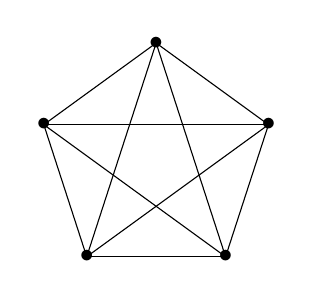
\begin{tikzpicture}[scale=1.5]
\foreach \i in {0, ..., 4}
	\draw (72*\i + 90:1) coordinate (x\i) node {$\bullet$};
\foreach \i in {0, ..., 3}
	\foreach \j in {\i, ..., 4}
		\draw (x\i) -- (x\j);
\end{tikzpicture}
\caption{Граф $K_5$}
\end{wrapfigure}

\index{Петля} Ребро вида $e = \{ u, u \}$ называется \textbf{петлёй}.

Рёбра, инцидентные одним и тем~же вершинам, называются \textbf{кратными}.

Граф называется \textbf{простым}, если он не содержит петель и кратных рёбер.

Граф, в~котором любые две вершины соединены ребром, называется \textbf{полным} и обозначается $K_n$, где $n$~--- число вершин в~нём.

Графы $G_1 = (V_1, E_1)$ и $G_2 = (V_2, E_2)$ называются \textbf{изоморфными}, если существует биекция~$\varphi \colon V_1 \to V_2$ такая, что
$\{ u, v \} \in E_1 \Leftrightarrow \{ \varphi(u), \varphi(v) \} \in E_2$, иначе~--- \textbf{неизоморфными}.
$\varphi$ называется \textbf{изоморфизмом}.

\index{Маршрут} \textbf{Маршрутом} в графе называется последовательность вершин и рёбер вида
$(v_1, e_1, v_2, \ldots, \allowbreak e_k, v_{k+1})$, где $e_i \opbr= \{ v_i, v_{i+1} \}$.

\index{Цепь} Маршрут, в~котором все рёбра различны, называется \textbf{цепью}.

Цепь, в~которой все вершины, за исключением, может быть, первой и последней, различны, называется \textbf{простой}.

Маршрут, в~котором первая и последняя вершины совпадают, называется \textbf{замкнутым}.

\index{Цикл} Замкнутая цепь называется \textbf{циклом}.

Маршрут, соединяющий вершины $u$ и $v$, называется \textbf{$(u, v)$"=маршрутом}.

\begin{lemma}
\label{lemma:walk_contains_simple_chain}
$(u, v)$-маршрут содержит $(u, v)$"=простую цепь.
\end{lemma}
\begin{proof}
Пусть $(u = v_1, e_1, v_2, \ldots, e_k, v_{k+1} = v)$~--- не простая цепь, тогда $\exists i < j \colon v_i = v_j$.
Уберём из маршрута подпоследовательность $(e_i, v_{i+1}, \ldots, e_{j-1}, v_j)$ и получим маршрут, в~котором совпадающих вершин на одну меньше.
Повторяя, получим простую цепь, являющуюся частью данного маршрута.
\end{proof}

\begin{lemma}
\label{lemma:cycle_contains_simple_one}
Любой цикл содержит простой цикл, причём каждая вершина и ребро цикла принадлежат некоторому простому циклу.
\end{lemma}
\begin{proof}
Пусть $(u = v_1, e_1, v_2, \ldots, e_k, v_{k+1} = u)$~--- не простой цикл, тогда $\exists i < j \colon v_i = v_j$.
Уберём из цикла подпоследовательность $(e_i, v_{i+1}, \ldots, e_{j-1}, v_j)$ и получим цикл, в~котором совпадающих вершин на одну меньше.
Повторяя, получим простой цикл, являющийся частью данного цикла.

Заметим, что подпоследовательность $(v_i, e_i, v_{i+1}, \ldots, e_{j-1}, v_j = v_i)$ также является циклом, из которого можно получить простой цикл.
Значит, некоторые вершины и рёбра этой подпоследовательности принадлежат простому циклу, остальные же снова образуют некоторые циклы, из которых можно получить простые.
Продолжая рассуждать таким образом, приходим к выводу, что любая вершина и ребро исходного цикла принадлежат некоторому простому циклу.
\end{proof}
	
\begin{lemma}
\label{lemma:existence_of_simple_cycle}
Если в~графе есть две различные простые цепи, соединяющие одни и те~же вершины, то в~этом графе есть простой цикл.
\end{lemma}
\begin{proof}
Пусть $(u = v_1, e_1, v_2, \ldots, e_n, v_{n+1} = v)$, $(u = v_1', e_1', v_2', \ldots, e_m', v_{m+1}' = v)$~--- простые цепи.
Найдём наименьшее~$i \colon e_i \neq e_i'$, тогда $(v_i, e_i, v_{i+1}, \ldots, e_n, v_{n+1} = v_{m+1}', e_m', \ldots, e_i', v_i' = v_i)$~--- цикл, значит, можно получить простой цикл.
\end{proof}

\subsection{Связность неориентированных графов}
Вершины $u$ и $v$ называются \textbf{связанными}, если существует $(u, v)$"=маршрут, иначе~--- \textbf{несвязанными}.

\index{Графы!связные} Граф называется \textbf{связным}, если в~нём любые две вершины связаны, иначе~--- \textbf{несвязным}.

Граф~$G' = (V', E')$ называется \textbf{подграфом графа~$G = (V, E)$}, если $V' \subseteq V \lAnd E' \subseteq E$.

\index{Компонента связности} \textbf{Компонентой связности графа} называется его максимальный относительно включения связный подграф.

\subsection{Эйлеровы графы}
Цикл, содержащий все рёбра графа, называется \textbf{эйлеровым}.

\index{Графы!эйлеровы} Граф, содержащий эйлеров цикл, называется \textbf{эйлеровым}.

\begin{theorem}
Связный граф эйлеров $\Leftrightarrow$ степени всех вершин чётны.
\end{theorem}
\begin{proof}
\begin{enumerate}
	\item $\Rightarrow$. Пусть в~графе есть эйлеров цикл.
	Выберем вершину~$v_0$ в~этом цикле и начнём обходить его.
	При каждом посещении вершины~$v \neq v_0$ её степень увеличивается на~$2$.
	Т.\,о., если посетить её $k$~раз, то $\deg v = 2k \mult 2$.
	
	Для $v_0$ степень увеличивается на~$1$ в~начале обхода, на~$1$ в~конце обхода и на~$2$ при промежуточных посещениях.
	Т.\,о., её степень чётна.
	
	\item $\Leftarrow$. Пусть степени всех вершин чётны.
	Выберём цепь~$C = (v_0, e_0, v_1, e_1, \ldots, e_{k-1}, v_k)$ наибольшей длины.
	Все рёбра, инцидентные~$v_k$, присутствуют в~этой цепи, иначе её можно было~бы удлинить.
	
	Докажем методом от противного, что $v_0 = v_k$.
	Пусть $v_0 \neq v_k$.
	При прохождении вершины~$v_i = v_k$, $i = 1, 2, \ldots, k - 1$, степень~$v_k$ увеличивается на~$2$.
	Также проходим по ребру~$e_{k-1}$, тогда степень~$v_k$ нечётна.
	Противоречие.
	
	Докажем методом от противного, что $C$ содержит все рёбра.	
	Пусть найдётся ребро~$e = \{ u, v \}$, не входящее в~$C$.
	Возьмём первое ребро~$e' = \{ v_i, v' \}$ из $(v_0, u)$"=маршрута, не входящее в~$C$.
	Тогда цепь~$(v', e', v_i, e_i, \ldots, e_{k-1}, \allowbreak v_k = v_0, \allowbreak e_0, v_1, e_1, \ldots, v_{i-1})$ длиннее, чем~$C$.
	Противоречие.
\end{enumerate}
\end{proof}

\subsubsection{Алгоритмы нахождения эйлерова цикла}
\paragraph{Алгоритм Флёри.}
\index{Алгоритм!Флёри} В качестве текущей вершины выберем произвольную.
\begin{enumerate}
	\item Выбираем ребро, инцидентное текущей вершине.
	Оно не должно быть мостом, если есть другие рёбра, не являющиеся мостами.
	\item Проходим по выбранному ребру и вычёркиваем его.
	Вершина, в~которой теперь находимся,~--- текущая.
	\item Повторяем с шага~1, пока есть рёбра.
\end{enumerate}

\paragraph{Алгоритм объединения циклов.}
\index{Алгоритм!объединения циклов}
\begin{enumerate}
	\item Выбираем произвольную вершину.
	\item Выбираем любое непосещённое ребро и идём по нему.
	\item Повторяем шаг~2, пока не вернёмся в~начальную вершину.
	\item Получили цикл~$C$.
	Если он не эйлеров, то $\exists u \in C, \ e = \{ u, u' \} \colon u' \notin C$.
	Повторяем шаги~2--3, начиная с вершины~$u$.
	Получили цикл~$C'$, рёбра которого не совпадают с рёбрами~$C$.
	Объединим эти циклы и получим новый.
	Повторяем шаг~4.
\end{enumerate}

Цепь называется \textbf{эйлеровым путём}, если она не является циклом и содержит все рёбра графа.

\index{Графы!полуэйлеровы} Граф называется \textbf{полуэйлеровым}, если в~нём есть эйлеров путь.

\begin{theorem}
Связный граф полуэйлеров $\Leftrightarrow$ степени двух вершин нечётны, а остальных~--- чётны.
\end{theorem}
\begin{proof}
\begin{enumerate}
	\item $\Rightarrow$. Пусть в~графе есть эйлеров путь.
	Соединив его концы ребром, получим эйлеров цикл.
	Степени соединённых вершин увеличились каждая на~$1$, значит, они были нечётными, а степени остальных вершин~--- чётными.
	\item $\Leftarrow$. Пусть степени двух вершин нечётны, а остальных~--- чётны.
	Соединим нечётные вершины ребром, тогда можно получить эйлеров цикл.
	Убрав из него добавленное ребро, получим эйлеров путь.
\end{enumerate}
\end{proof}

\subsection{Гамильтоновы графы}
Простой цикл, содержащий все вершины графа, называется \textbf{гамильтоновым}.

\index{Графы!гамильтоновы} Граф называется \textbf{гамильтоновым}, если в~нём есть гамильтонов цикл.

\index{Теорема!Оре}
\begin{theorem}[Оре]
Если в~графе с $n \geqslant 3$~вершинами для любых двух несмежных вершин $u$ и $v$ $\deg u \opbr+ \deg v \opbr\geqslant n$, то граф гамильтонов.
\end{theorem}
\begin{proof}
\begin{enumerate}
	\item Докажем методом от противного, что граф связный.
	Пусть он несвязный, тогда в~нём найдутся хотя~бы две компоненты связности $G_1(V_1, E_1)$ и $G_2(V_2, E_2)$.
	Пусть $u \in V_1$, $v \in V_2$.
	$u$ и $v$ несмежные, тогда
	\begin{equation*}
	\deg u \leqslant |V_1| - 1, \ \deg v \leqslant |V_2| - 1 \Rightarrow \deg u + \deg v \leqslant |V_1| + |V_2| - 2 \leqslant n - 2
	\end{equation*}
	
	Противоречие с условием.
	
	\item Докажем, что граф гамильтонов.
	Выберем цепь~$W = (v_0, e_0, v_1, \ldots, e_{k-1}, v_k)$ наибольшей длины.
	В~ней содержатся все вершины, соседние с~$v_0$ или с~$v_k$.
	Т.\,о., среди вершин $v_1, \ldots, v_k$ находится ровно $\deg v_0$ соседних с~$v_0$ вершин.
	Аналогично для $v_k$.
	
	$\deg v_0 + \deg v_k \geqslant n$, тогда найдутся $v_i$ и $v_{i+1}$ такие, что $v_i$ соседняя с~$v_k$, а $v_{i+1}$~--- с~$v_0$.
	
	Докажем, что $(v_{i+1}, e_{i+1}, \ldots, v_k, e, v_i, e_{i-1}, v_{i-1}, \ldots, e_0, v_0, e', v_{i+1})$~--- гамильтонов цикл, методом от противного.
	Предположим обратное, тогда есть вершина~$u$, не входящая в~цикл, и существует $(v_0, u)$"=маршрут.
	Значит, существует ребро, инцидентное одной из вершин цикла, но не входящее в~него, и можно получить более длинную цепь.
	Противоречие, значит, $G$~--- гамильтонов граф.
\end{enumerate}
\end{proof}

\index{Теорема!Дирака}
\begin{theorem}[Дирака]
\label{th:Dirac}
Если в графе~$G = (V, E)$ с $n \geqslant 3$~вершинами $\forall u \in V \ \deg u \geqslant \frac{n}2$, то граф гамильтонов.
\end{theorem}
\begin{proof}
Пусть $u$, $v$~--- несвязные вершины в~$G$, тогда $\deg u \geqslant \frac{n}2 \lAnd \deg v \geqslant \frac{n}2 \Rightarrow \deg u + \deg v \geqslant n$ $\Rightarrow$ по теореме Оре $G$ гамильтонов.
\end{proof}

Цепь называется \textbf{гамильтоновым путём}, если она не является циклом и содержит все вершины графа.

\index{Графы!полугамильтоновы} Граф называется \textbf{полугамильтоновым}, если в нём есть гамильтонов путь.

\subsection{Планарность графов}
\index{Графы!плоские} \textbf{Плоским} называется граф~$G = (V, E)$ такой, что:
\begin{itemize}
	\item $V \subset \mathbb R^2$;
	\item рёбра~--- кривые, концами которых являются вершины;
	\item различные рёбра не имеют общих точек, за исключением концов.
\end{itemize}

\index{Графы!планарные} \textbf{Планарным} называется граф, изоморфный плоскому.

Если $G$~--- граф и $G'$~--- плоский граф, изоморфный $G$, то $G'$ называется \textbf{укладкой $G$} в~$\mathbb R^2$.

Аналогично можно определить плоский граф в~$\mathbb R^3$, на~сфере и~т.\,д.

\begin{theorem}
Любой граф можно уложить в~$\mathbb R^3$.
\end{theorem}
\begin{proof}
Пусть $G = (V, E)$~--- граф, $V = \{ (1, 0, 0), (2, 0, 0), \ldots, (n, 0, 0) \}$.
Рассмотрим плоскости, проходящие через~$Ox$ и образующие с плоскостью~$Oxy$ углы
$\dfrac\pi2, \dfrac\pi{2\cdot2}, \ldots, \dfrac\pi{2m}$, где $m = |E|$.
В каждой такой плоскости можно провести ровно одно ребро, тогда получим плоский граф, т.\,к. плоскости пересекаются только по прямой~$Ox$.
\end{proof}

\begin{theorem}
Граф укладывается на~плоскость $\Leftrightarrow$ он укладывается на~сферу.
\end{theorem}
\begin{proof}
Пусть плоскость~$z = 0$ касается сферы в точке~$O(0, 0, 0)$, $N$~--- точка на~сфере, диаметрально противоположная точке~$O$.
Для каждой точки сферы, не совпадающей с~$N$, проведём прямую через неё и точку~$N$, которая пересечёт сферу и плоскость, причём любые две из таких прямых имеют единственную общую точку~$N$.
Получим биекцию между точками сферы и точками плоскости, тогда можно построить биекцию между укладками на сфере и укладками на плоскости.
\end{proof}

\begin{center}
\noindent
\shorthandoff{"}
\begin{tikzpicture}[>=stealth]
% рисуем оси
\def\tilt_angle{60}
\draw[->] (0, 0) coordinate["$O$" {below right}] (O) node {$\bullet$}
	+(\tilt_angle:3.5) -- +(\tilt_angle-180:2.5) node[below right] {$x$};
\draw[->] (-4, 0) -- (4.5, 0) node[below] {$y$};
\draw[->] (0, -1.3) -- (0, 4) node[left] {$z$};

% рисуем сферу
\def\radius{1.5}
\draw[name path=sphere] (0, \radius) circle (\radius);

% рисуем плоскость
\def\lenAB{4}
\draw (-4, -1.5) coordinate (A) -- ++(\tilt_angle:\lenAB) coordinate (B);
\draw (A) -- (2, -1.5) coordinate (D) -- ++(\tilt_angle:\lenAB) coordinate (C);
\path[name path=BC] (B) -- (C);
\draw[name intersections={of=BC and sphere, name=i}]
	(B) -- (i-2) (i-1) -- (C);
\draw[dashed] (i-1) -- (i-2);

% рисуем прямую
\draw[dashed] (0, 2*\radius) node[above right] {$N$} node {$\bullet$} -- (-0.6, 0.75) coordinate (point) node {$\bullet$};
\draw (point) -- (-1.15, -1) node {$\bullet$};
\end{tikzpicture}
\shorthandon{"}
\end{center}

Множество на плоскости называется \textbf{линейно связным}, если любые две точки этого множества можно соединить кривой, целиком лежащей в~этом множестве.

\index{Грань} \textbf{Гранью плоского графа~$G = (V, E)$} называется часть множества~$\mathbb R^2 \setminus G$, которая линейно связна и не является подмножеством другого линейно связного множества.

\index{Формула!Эйлера!в~теории графов}
\begin{theorem}[формула Эйлера]
В~плоском связном графе $n - m + f = 2$, где $n, m, f$~--- число вершин, рёбер и граней соответственно.
\end{theorem}
\begin{proof}
Рассмотрим остов данного графа.
В~нём $n$~вершин, $n - 1$~рёбер и $1$~грань.
Формула Эйлера верна для него: $n - (n - 1) + 1 = 2$.

Добавим $1$~ребро данного графа, тогда оно разобьёт одну грань на две, т.\,е. число граней увеличится на~$1$.
Формула Эйлера верна для полученного графа.
Повторяя $m - (n - 1)$~раз, получим исходный граф, для которого формула Эйлера верна.
\end{proof}

\begin{theorem}
\label{th:property_of_planarity_of_graph}
Пусть $G$~--- планарный граф с $n \geqslant 3$~вершинами и $m$~рёбрами. Тогда $m \leqslant 3n - 6$.
\end{theorem}
\begin{proof}
При $m = 2$ неравенство выполняется.

Пусть в~графе $f$~граней, $m_i$~--- число рёбер в~границе $i$-й грани.
Тогда $m_i \geqslant 3$, $\sum\limits_{i=1}^f m_i \geqslant 3f$.
С~другой стороны, $\sum\limits_{i=1}^f m_i \leqslant 2m$, т.\,к. каждое ребро является границей для не более чем $2$ граней.
По формуле Эйлера $n - m + f = 2 \Leftrightarrow f = m + 2 - n$.
Получим:
\begin{equation*}
2m \geqslant 3f \Leftrightarrow 2m \geqslant 3m + 6 - 3n \Leftrightarrow m \leqslant 3n - 6
\end{equation*}
\end{proof}

\begin{consequent}
Планарный граф~$G = (V, E)$ содержит хотя~бы одну вершину со~степенью, не большей~$5$.
\end{consequent}
\begin{proofcontra}
Пусть $\forall v \in V \ \deg v \geqslant 6$, $|V| = n$, $|E| = m$, тогда
$m \opbr= \frac12 \sum\limits_{v \in V} \deg v \opbr\geqslant 3n$.
Имеем:
\begin{equation*}
3n \leqslant m \leqslant 3n - 6 \Rightarrow 0 \leqslant -6
\end{equation*}

Противоречие.
\end{proofcontra}

\begin{theorem}
Графы $K_5$ и $K_{3,3}$ не планарные.
\end{theorem}
\begin{proof}
\begin{itemize}
	\item Рассмотрим $K_5$.
	Для него $n = 5$, $m = 10$.
	Тогда $m \leqslant 3n - 6 \Leftrightarrow 10 \leqslant 9$.	
	Неверно, значит, $K_5$ не планарен.
	\item Рассмотрим $K_{3,3}$.
	Пусть он планарный.
	В~нём самый короткий цикл имеет длину~$4$.
	Тогда рассуждениями, аналогичными рассуждениям при доказательстве теоремы~\ref*{th:property_of_planarity_of_graph}, получим
	\begin{equation*}
	2m \geqslant 4f \Leftrightarrow 2m \geqslant 4m + 8 - 4n \Leftrightarrow m \leqslant 2n - 4
	\end{equation*}
	
	Для $K_{3,3}$ $n = 6$, $m = 9$, тогда $9 \leqslant 8$.
	Неверно, значит, $K_{3,3}$ не планарен.
\end{itemize}
\end{proof}

Граф~$G' = (V', E')$ получается \textbf{подразбиением ребра~$e = \{ u, v \}$} графа~$G = (V, E)$, если:
\begin{itemize}
	\item $V' = V \cup \{ u' \}$;
	\item $E' = (E \setminus \{ e \}) \cup \{ \{ u, u' \}, \{ v, u' \} \}$.
\end{itemize}

\index{Графы!гомеоморфные} Графы $G$ и $G'$ \textbf{гомеоморфны}, если они изоморфны графам, получающимся подразбиениями рёбер одного и того~же графа.

\index{Теорема!Понтрягина---Куратовского}
\begin{theorem}[Понтрягина"--~Куратовского]
Граф~$G$ планарен $\Leftrightarrow$ он не содержит подграфов, гомеоморфных $K_5$ или $K_{3,3}$.
\end{theorem}
\begin{proof}
\begin{enumerate}
	\item $\Rightarrow$. Очевидно, что подграф планарного графа планарен.
	Если $G$~--- планарный граф, содержащий подграф $G'$, гомеоморфный $K_5$ или $K_{3,3}$, то $G'$ тоже планарный, значит, $K_5$ или $K_{3,3}$ планарен, т.\,к. подразбиение ребёр не влияет на планарность.
	Противоречие, значит, $G$ не планарен.
	\item $\Leftarrow$. Доказательство слишком сложно, поэтому здесь не приводится.
\end{enumerate}
\end{proof}

\subsection{Деревья}
\index{Лес} Граф без циклов называется \textbf{лесом}.

\index{Дерево} Связный лес называется \textbf{деревом}.

\index{Мост} Ребро называется \textbf{мостом}, если при его удалении увеличивается число компонент связности.

\begin{statement}
\label{st:criterion_of_bridge_in_graph}
Ребро~--- мост $\Leftrightarrow$ оно не содержится в~цикле.
\end{statement}
\begin{proof}
\begin{enumerate}
	\item $\Leftarrow$.
	Пусть ребро $e$ содержится в цикле $W = (v_0, e_0, \ldots, u, e, v, \ldots, v_k)$, $u'$ и $v'$~--- связные вершины.
	\begin{enumerate}
		\item Если в~$(u', v')$"=маршруте нет ребра~$e$, то при его удалении из графа $u'$ и $v'$ останутся связными.
		\item Пусть $(u' = v_0', e_0', \ldots, u, e, v, \ldots, e_m', v_m' = v')$~--- маршрут, соединяющий $u'$ и $v'$, тогда при удалении $e$ из графа $u'$ и $v'$ соединяет маршрут
		$(u' = v_0', e_0', \ldots, u, \ldots, e_0, v_0 = v_k, e_{k-1}, \ldots, v, \ldots, e_m', v_m' = v')$.
	\end{enumerate}
	
	\item $\Rightarrow$.
	Пусть $e = \{ u, v \}$ не является мостом, тогда $u$, $v$ лежат в~одной компоненте связности.
	Удалим $e$ из графа.
	Число компонент связности не изменится, значит, $u$ и $v$ также лежат в~одной компоненте связности, т.\,е. существует цепь, соединяющая $u$ и $v$: $(u = v_0, e_0, \ldots, e_{k-1}, v_k = v)$.
	Тогда в~исходном графе существует цикл $(u = v_0, e_0, \ldots, e_{k-1}, v_k = v, e, u)$.
\end{enumerate}
\end{proof}

\begin{theorem}
Следующие утверждения о графе~$G = (V, E)$ с~$n$ вершинами эквивалентны:
\begin{enumerate}
	\item $G$~--- дерево.
	\item $G$ связный и каждое его ребро~--- мост.
	\item $G$ связный и имеет $n - 1$~ребро.
	\item $G$ не содержит циклов и имеет $n - 1$~ребро.
	\item Любые две вершины графа~$G$ соединены ровно одной простой цепью.
	\item $G$ не содержит циклов и добавление ребра приводит к появлению ровно одного цикла.
\end{enumerate}
\end{theorem}
\begin{proof}
\begin{itemize}
	\item 1 $\Rightarrow$ 2.
	Связность следует из определения дерева.
	
	В~силу утверждения~\ref*{st:criterion_of_bridge_in_graph} каждое ребро~--- мост.
	
	\item 2 $\Rightarrow$ 3.
	Связность следует из предположения.
	
	Докажем методом математической индукции, что в~графе $n - 1$~ребро.
	\indbase Для $n = 1, 2$ очевидно.
	\indstep Пусть утверждение верно для чисел, меньших $n$.
	Возьмём мост~$e$ и удалим его.
	Получим две компоненты связности $G_1 = (V_1, E_1)$, $G_2 = (V_2, E_2)$.
	По предположению индукции $|E_1| = |V_1| - 1$, $|E_2| = |V_2| - 1$.
	Тогда в~исходном графе рёбер $|E_1| + |E_2| + 1 = |V_1| + |V_2| - 1 = n - 1$. \indend
	
	\item 3 $\Rightarrow$ 4.
	$G$ имеет $n - 1$~ребро по предположению.
	
	Докажем методом математической индукции, что $G$ не содержит циклов.
	\indbase Для $n = 1, 2$ очевидно.
	\indstep Пусть утверждение верно для чисел, меньших $n$.
	Докажем методом от противного, что в~графе есть вершина степени~$1$.
	Пусть
	\begin{equation*}
	\forall u \in V \ \deg u \geqslant 2 \Rightarrow 2|E| = \sum_{u \in V} \deg u \geqslant 2n \Rightarrow n - 1 = |E| \geqslant n \Rightarrow -1 \geqslant 0
	\end{equation*}
	Противоречие, значит, в~графе найдётся вершина степени~$1$.
	
	Удалим её и инцидентное ей ребро.
	Полученный граф содержит $n - 1$~вершину и удовлетворяет утверждению~3.
	По предположению индукции он не содержит циклов, тогда и исходный граф не содержит циклов. \indend
	
	\item 4 $\Rightarrow$ 5.
	
	Пусть в~графе $k$~компонент связности: $G_1 = (V_1, E_1)$, $G_2 = (V_2, E_2)$, \ldots, $G_k = (V_k, E_k)$.
	Они не содержат циклов по предположению, тогда они являются деревьями.
	\begin{equation*}
	|E_1| = |V_1| - 1 \lAnd |E_2| = |V_2| - 1 \lAnd \ldots \lAnd |E_k| = |V_k| - 1 \lAnd 
	n - 1 = |E_1| + \ldots + |E_k| = n - k \Rightarrow k = 1
	\end{equation*}
	Значит, граф связный.
	
	Пусть существуют вершины $u$ и $v$ такие, что их соединяют две простые цепи, тогда по лемме~\ref{lemma:existence_of_simple_cycle} в~графе есть цикл, что противоречит предположению.
	Значит, эти вершины соединены ровно одной простой цепью.
	
	\item 5 $\Rightarrow$ 6.
	
	Докажем методом от противного, что в~графе нет циклов.
	Предположим, что есть цикл $(v_0, e_0, v_1, \ldots, v_k = v_0)$, тогда есть две простые цепи $(v_0, e_0, \ldots, v_{k-1})$ и $(v_{k-1}, e_k, v_k = v_0)$, соединяющие $v_0$ и $v_{k-1}$, что противоречит предположению.
	
	Докажем, что добавление ребра приводит к появлению ровно одного цикла.
	Рассмотрим несоседние вершины $u$ и $v$.
	По предположению есть цепь $(u = v_0, e_0, \ldots, v_k = v)$, соединяющая их.
	Тогда, добавив $e = \{ u, v \}$, получим цикл $(u = v_0, e_0, \ldots, v_k = v, e, u)$.
	
	Пусть есть $2$~цикла, соединяющих $u$ и $v$.
	Удалим $e$, тогда один цикл останется.
	Получим исходный граф, в~котором не должно быть циклов.
	Противоречие.
	
	\item 6 $\Rightarrow$ 1.
	
	Докажем связность методом от противного.
	Рассмотрим несвязные вершины $u$ и~$v$.
	Соединим их и по~предположению получим цикл $(v_0, e_0, \ldots, u, e, v, \ldots, e_{k-1}, v_k = v_0)$.
	Тогда в~исходном графе $(u, \ldots, e_0, v_0 = v_k, \allowbreak e_{k-1}, \ldots, v)$~--- $(u, v)$"=маршрут.
	Противоречие.
\end{itemize}
\end{proof}

В~ходе доказательства было получено, что в~связном графе с $n$~вершинами и $n - 1$~рёбрами существует висячая вершина.
Т.\,к. доказано, что такой граф является деревом, то верно следующее утверждение.
\begin{statement}
В~дереве существует висячая вершина.
\end{statement}

\begin{statement}
Если в лесу $n$~вершин, $m$~рёбер и $k$~компонент связности, то $m = n - k$.
\end{statement}
\begin{proof}
Пусть $n_1, \ldots, n_k$~--- число вершин в каждой компоненте связности, тогда
\begin{equation*}
m = (n_1 - 1) + (n_2 - 1) + \ldots + (n_k - 1) = n - k
\end{equation*}
\end{proof}

\subsection{Остовы}
\index{Остов} \textbf{Остовом графа $G = (V, E)$} называется его подграф~$G' = (V', E') \colon V = V' \lAnd G'$~--- дерево.

\begin{statement}
Любой связный граф содержит остов.
\end{statement}

\begin{statement}
Если граф не является деревом, то в~нём несколько остовов.
\end{statement}

Пусть $G = (V, E)$~--- граф.

\index{Вес} \textbf{Весом} называется функция~$\alpha \colon E \to \mathbb R^+$.

\textbf{Весом ребра}~$e \in E$ называется $\alpha(e)$.

\textbf{Весом графа} называется $\sum\limits_{e \in E} \alpha(e)$.

Пусть дан граф~$G = (V, E)$, $n = |V|$ и весовая функция $\alpha \colon E \to R^+$, и необходимо найти остов наименьшего веса $T = (V, P)$.

\subsubsection{Алгоритм Краскала}
\index{Алгоритм!Краскала}
\begin{enumerate}
	\item[1.] Выбираем ребро~$e \in E$ с наименьшим весом: $P_1 = \{ e \}$, $T_1 = (V, P_1)$.
	\item[i.] Выбираем ребро~$e \in E$ с наименьшим весом такое, что $e \notin P_i$ и добавление этого ребра не приводит к образованию цикла в~$T$: $T_{i+1} = (V, P_i \cup \{ e \})$.
\end{enumerate}

$T_n$~--- искомый остов.
\begin{proof}[корректности]
	Пусть $T = (V, P)$~--- построенный остов, где
	$P = \{ e_1, e_2, \ldots, e_{n-1} \}$, $e_1, e_2, \ldots, \allowbreak e_{n-1}$~--- рёбра в~порядке их добавления в~остов, а также $D = (V, M)$~--- другой остов, где
	$M = \{ e_1', e_2', \ldots, e_{n-1}' \}$, $e_1', e_2', \ldots, e_{n-1}'$~--- рёбра в~порядке неубывания их весов.
	
	Если $T \neq D$, то пусть $i$~--- наименьшее число такое, что $e_i \neq e_i'$.
	$e_i'$ не входит в~$T$, значит, оно образует цикл с рёбрами в~$T$, выбранными ранее, тогда вес этих рёбер не больше $\alpha(e_i')$.
	Выберем из них ребро~$e$ такое, что при добавлении его в~$D$ образуется цикл.
	Пусть $D_1 = (V, M \cup \{ e \} \setminus \{ e_i' \})$.
	Этот граф~--- остов, причём вес~$D_1$ не больше веса~$D$ и у~$T$ и $D_1$ на~$1$ общее ребро больше, чем у~$T$ и $D$.
	Повторяя, получим $D_k = T$.
	Значит, вес построенного остова не превосходит веса любого другого остова.
\end{proof}

\subsubsection{Алгоритм Прима}
\index{Алгоритм!Прима}
Строится последовательность деревьев $S_1 \subset S_2 \subset \ldots \subset S_n = T$.
\begin{enumerate}
	\item[1.] Выбираем произвольную вершину~$v$.
	$S_1 = (\{ v \}, \varnothing)$.
	\item[i.] Пусть построено $S_{i-1} = (V_{i-1}, E_{i-1})$.
	Находим ребро~$e = \{ u, v_{i-1} \} \in E$, где $u \in V_{i-1}$, $v_{i-1} \notin V_{i-1}$, наименьшего веса, добавление которого не приводит к образованию цикла: $S_i = (V_{i-1} \cup \{ v_{i-1} \}, E_{i-1} \cup \{ e \})$.
\end{enumerate}

$S_n$~--- искомый остов.

\subsection{Помеченные деревья}
\index{Дерево!помеченное} Дерево с $n$~вершинами, которым сопоставлены числа~$1, \ldots, n$, называется \textbf{помеченным}.

\index{Код Прюфера} Каждому помеченному дереву можно взаимнооднозначно сопоставить последовательность из $n - 2$~чисел от $1$ до $n$, называемую \textbf{кодом Прюфера}.
Алгоритм построения кода Прюфера для помеченного дерева~$G = (V, E)$:
\begin{enumerate}
	\item Выбираем висячую вершину~$v$ с наименьшим номером.
	\item Добавляем номер вершины, смежной с~$v$, в~код.
	\item Удаляем~$v$ и ребро, инцидентное $v$, из дерева.
	\item Повторить, начиная с шага~1, $n - 2$~раза.
\end{enumerate}

\begin{statement}
Различным помеченным деревьям соответствуют различные коды Прюфера.
\end{statement}
\begin{proofmathind}
	\indbase При $n = 3$ легко проверить.
	\indstep Пусть утверждение верно при $n$, $G = (V, E)$ и $G' = (V', E')$~--- различные помеченные деревья с $n + 1$~вершинами в~каждом.
	Если в $G$ и $G'$ вершины с наименьшим номером смежны с вершинами с одинаковыми номерами, то выполняем шаг построения кода, тогда оставшиеся деревья различны, значит, по предположению индукции у них различные коды. \indend
\end{proofmathind}

Алгоритм построения дерева по коду $A_0 = (a_0, \ldots, a_{n-3})$:

Пусть $B_0 = \{ 1, \ldots, n \}$.
\begin{enumerate}
	\item Находим наименьшее $b \in B_i \colon b \notin A_i$.
	Тогда в~дереве есть ребро $\{ b, a_i \}$: $A_{i+1} = A_i \setminus \{ a_i \} \lAnd B_{i+1} = B_i \setminus \{ b \}$.
	\item Повторяем шаг~1 $n - 2$~раз.
	Получим $B_{n-2} = \{ b', b'' \}$, значит, в~дереве есть ребро~$\{ b', b'' \}$.
\end{enumerate}

Докажем, что указанный алгоритм по коду из $n$~чисел строит дерево.
\begin{proofmathind}
	\indbase При $n = 1$ легко проверить.
	\indstep Рассмотрим графы $T_1, \ldots, T_{n-1}$, полученные в~процессе построения дерева.
	$T_1$ не содержит циклов.
	$T_2$ получается из $T_1$ либо добавлением новой вершины, либо добавлением моста, что не приводит к появлению цикла.	
	По индукции получим, что $T_{n-1}$ не содержит циклов и содержит $n$~вершин и $n - 1$~ребёр, значит, $T_{n-1}$~--- дерево.
	\indend
\end{proofmathind}

\index{Теорема!Кэли}
\begin{theorem}[Кэли]
Количество неизоморфных помеченных деревьев с $n$~вершинами равно~$n^{n-2}$.
\end{theorem}
\section{Ориентированные графы}
\index{Графы!ориентированные} \textbf{Ориентированным графом} называется пара~$(V, E)$, где $V$~--- непустое конечное множество, $E$~--- совокупность элементов множества~$V^2$.
Элементы~$V$ называются \textbf{вершинами графа}.
Элементы~$E$ называются \textbf{дугами графа}.

На рисунках ориентированные графы изображаются так же, как неориентированные, за тем исключением, что на дуги дополнительно наносятся стрелки, направленные от начальной вершины к конечной.

Если $e = (u, v) \in E$, то говорят, что:
\begin{itemize}
	\item дуга~$e$ выходит из вершины~$u$ и входит в вершину~$v$;
	\item $u$~--- начало дуги~$e$, а $v$~--- её конец;
	\item дуга~$e$ инцидентна вершинам $u$ и $v$;
	\item вершины $u$ и $v$ инцидентны дуге~$e$.
\end{itemize}

\index{deg} Количество выходящих из вершины~$v$ дуг называется \textbf{полустепенью исхода вершины} и обозначается $\deg_+ v$.

Количество входящих в вершину~$v$ дуг называется \textbf{полустепенью захода вершины} и обозначается $\deg_- v$.

Количество инцидентных вершине~$v$ дуг называется \textbf{степенью вершины} и обозначается $\deg v$.
Очевидно, что $\deg v = \deg_+ v + \deg_- v$.

\begin{statement}
\begin{equation*}
\sum_{v \in V} \deg_+ v = \sum_{v \in V} \deg_- v = |E|
\end{equation*}
где $(V, E)$~--- граф.
\end{statement}
\begin{proof}
Достаточно заметить, что каждая дуга увеличивает полустепень исхода некоторой вершины на $1$ и полустепень захода некоторой вершины на $1$.
\end{proof}

\index{Петля} Дуга~$e = (u, u)$ называется \textbf{петлёй}.

Если в графе есть несколько дуг~$(u, v)$, то они называются \textbf{кратными}.

Дуги $(u, v)$ и $(v, u)$ называются \textbf{противоположно направленными}.

Граф называется \textbf{простым}, если в нём нет пётель и кратных дуг.

Граф~$(V_1, E_1)$ называется \textbf{подграфом графа~$(V, E)$}, если $V_1 \subseteq V \lAnd E_1 \subseteq E$.

Неориентированный граф, полученный из ориентированного графа~$G$ заменой дуг на рёбра, называется \textbf{основанием графа~$G$}. 

Графы $G_1 = (V_1, E_1)$ и $G_2 = (V_2, E_2)$ называются \textbf{изоморфными}, если существует биекция~$\varphi \colon V_1 \to V_2$ такая, что
$(u, v) \in E_1 \Leftrightarrow (\varphi(u), \varphi(v)) \in E_2$, иначе~--- \textbf{неизоморфными}.

\index{Путь} \textbf{Путём} в графе называется последовательность $(v_1, e_1, v_2, e_2, \ldots, v_{k-1}, e_k, v_k)$ его вершин и дуг такая, что $e_i \opbr= (v_i, v_{i+1})$.

Путь называется \textbf{простым}, если в нём все вершины, кроме, возможно, первой и последней, различны.

Путь называется \textbf{замкнутым}, если в нём первая и последняя вершины совпадают.

\index{Контур} Замкнутый путь называется \textbf{контуром}.

Путь, соединяющий вершины $u$ и $v$, называется \textbf{$(u, v)$"=путём}.

Если в графе существует $(u, v)$"=путь, то говорят, что вершина~$v$ \textbf{достижима} из вершины~$u$.
Если также существует $(v, u)$"=путь, то говорят, что вершины $u$ и $v$ \textbf{взаимодостижимы}.

\begin{lemma}
Любой путь содержит простой путь.
\end{lemma}%
Доказательство аналогично доказательству леммы~\ref{lemma:walk_contains_simple_chain}.

\begin{lemma}
Любой контур содержит простой контур, причём каждая вершина и дуга контура принадлежат некоторому простому контуру.
\end{lemma}%
Доказательство аналогично доказательству леммы~\ref{lemma:cycle_contains_simple_one}.

\subsection{Связность ориентированных графов}
Ориентированный граф называется \textbf{сильно связным}, если для любых его вершин $u$ и $v$ существуют $(u, v)$"=путь и $(v, u)$"=путь.

Ориентированный граф называется \textbf{слабо связным}, если связно его основание.

\index{Теорема!Роббинса}
\begin{theorem}[Роббинса]
Связный неориентированный граф обладает сильно связной ориентацией $\Leftrightarrow$ он не содержит мостов.
\end{theorem}
\begin{proof}
\begin{enumerate}
	\item $\Rightarrow$. Если граф содержит мост~$\{ u, v \}$, то при его ориентации можно получить либо дугу~$(u, v)$, либо дугу~$(v, u)$.
	В таком случае одна из компонент связности, соединяемых мостом, будет недостижима из другой.
	
	\item $\Leftarrow$. Любое ребро принадлежит некоторому циклу~$C$, так как оно не является мостом.
	Ориентируем все рёбра цикла в одну сторону.
	Если остались другие рёбра, то в силу связности графа можно получить ещё один цикл, часть которого является частью цикла~$C$.
	Ориентируем все рёбра полученного цикла в одну сторону, не изменяя уже ориентированные рёбра.
	Повторяя, ориентируем все рёбра графа.
	
	Для любых двух вершин $u$ и $v$ исходного графа существует маршрут $(u = v_1, e_1, \ldots, e_{k-1}, v_k = v)$.
	Чтобы получить $(u, v)$"=путь, идём по дугам $(v_1, v_2)$, $(v_2, v_3)$ и т.\,д.
	Если дуги $(v_i, v_{i+1})$ нет, то есть дуга $(v_{i+1}, v_i)$, состоящая в некотором цикле, пройдя по которому, можно из вершины~$v_i$ попасть в вершину~$v_{i+1}$.
	
	Аналогично получим $(v, u)$"=путь.
\end{enumerate}
\end{proof}

\index{Компонента связности} \textbf{Компонентой сильной связности} ориентированного графа называется максимальный относительно включения сильно связный подграф.
Аналогично определяется \textbf{компонента слабой связности}.

\textbf{Конденсацией ориентированного графа} называется ориентированный граф, вершинами которого являются компоненты сильной связности исходного графа, а дуга между вершинами показывает наличие пути между вершинами компонент.

\begin{statement}
Конденсация не содержит контуров.
\end{statement}
\begin{proofcontra}
Предположим, что в конденсации существует контур.
Тогда очевидно, что вершины различных компонент, входящих в него, взаимодостижимы, а значит, лежат в одной компоненте сильной связности.
Противоречие.
\end{proofcontra}

\subsection{Способы задания ориентированного графа}
Пронумеруем вершины графа~$G = (V, E)$, т.\,е. зададим биекцию $\varphi \colon V \to \{ 1, 2, \ldots, n \}$, где $n = |V|$, и будем их обозначать $1, 2, \ldots, n$.

\subsubsection{Матрица смежности}
\index{Матрица!смежности} \textbf{Матрицей смежности графа~$G$} называется матрица $A = \|a_{ij}\|_{\begin{smallmatrix}
i = \overline{1,n} \\
j = \overline{1,n}
\end{smallmatrix}}$, где $a_{ij}$ равно числу рёбер~$(i, j)$ в графе.

\begin{theorem}
Если $A = \|a_{ij}\|_{\begin{smallmatrix}
i = \overline{1,n} \\
j = \overline{1,n}
\end{smallmatrix}}$~--- матрица смежности графа~$G$,
$A^k = \|b_{ij}\|_{\begin{smallmatrix}
i = \overline{1,n} \\
j = \overline{1,n}
\end{smallmatrix}}$, то $b_{ij}$ равно числу $(i, j)$-путей длины~$k$.
\end{theorem}
\begin{proofmathind}
	\indbase Для $k = 1$ истинность следует из определения.
	\indstep Пусть теорема верна для $k$, $A^{k+1} = \|c_{ij}\|_{\begin{smallmatrix}
	i = \overline{1,n} \\
	j = \overline{1,n}
	\end{smallmatrix}}$.
	\begin{equation*}
	A^{k+1} = A A^k \Rightarrow c_{ij} = \sum_{l=1}^n a_{il} b_{lj}
	\end{equation*}
	
	Значение выражения $a_{il} b_{lj}$, очевидно, равно числу $(i, j)$"=путей длины~$k + 1$, проходящих по дуге~$(i, l)$ (если таких дуг нет в графе, то выражение равно $0$).
	Тогда, суммируя эти выражения по всем~$l$, получим число всех $(i, j)$"=путей длины $k + 1$. \indend
\end{proofmathind}

\subsubsection{Матрица инцидентности}
Так же, как и вершины, пронумеруем дуги графа~$G$ и будем их обозначать $1, 2, \ldots, m$.

\index{Матрица!инцидентности} \textbf{Матрицей инцидентности графа~$G$} называется матрица $A = \|a_{ij}\|_{\begin{smallmatrix}
i = \overline{1,n} \\
j = \overline{1,m}
\end{smallmatrix}}$, где
\begin{equation*}
a_{ij} =
\begin{cases}
-1, \ \text{вершина~$i$~--- конец дуги~$j$} \\
0, \ \text{вершина~$i$ не инцидентна дуге~$j$} \\
1, \ \text{вершина~$i$~--- начало дуги~$j$}
\end{cases}
\end{equation*}

\subsection{Взвешенные графы}
Граф~$(V, E)$ называется \textbf{взвешенным}, если задана функция~$w \colon E \to R^+$, называемая \textbf{весом}.

\textbf{Весом дуги~$e \in E$} называется $w(e)$.

\textbf{Весом}, или \textbf{длиной}, \textbf{пути} называется сумма весов входящих в него дуг.

$(u, v)$"=путь называется \textbf{кратчайшим}, если он имеет наименьший вес среди всех $(u, v)$"=путей.

Наименьший вес среди всех $(u, v)$"=путей называется \textbf{расстоянием между вершинами $u$ и $v$} и обозначается $d(u, v)$.

\begin{statement}
$d(u, v) \leqslant d(u, k) + d(k, v)$, причём $d(u, v) = d(u, k) + d(k, v)$ $\Leftrightarrow$ $k$ лежит на одном из кратчайших $(u, v)$"=путей.
\end{statement}
\begin{proof}
Пусть $p_1$ и $p_2$~--- кратчайшие $(u, k)$"=путь и $(k, v)$"=путь соответственно.
Тогда $p_1 \cup p_2$~--- $(u, v)$"=путь.
Значит, либо этот путь кратчайший и его вес минимален (в таком случае $d(u, v) = d(u, k) + d(k, v)$), либо его вес больше, чем $d(u, v)$ (в этом случае ни один из кратчайших $(u, v)$"=путей не проходит через вершину~$k$).
\end{proof}

Пусть дан граф~$(V, E)$ и вес~$w \colon E \to R^+$.

\subsubsection{Алгоритм Дейкстры}
\index{Алгоритм!Дейкстры} Алгоритм Дейкстры ищет длины кратчайших путей между некоторой вершиной~$u$ и всеми остальными.
Каждой вершине~$v$ на шаге~$i$ сопоставим метки~$l_i(v) \geqslant d(u, v)$.
\begin{enumerate}
	\item[0.] $l_0(u) = 0$, $\forall v \in V \ v \neq u \Rightarrow l_0(v) = \infty$
	\item[k.] Пусть $m$~--- непосещённая вершина с минимальным~$l_{k-1}(m)$.
	Отметим $m$ как посещённую.
	\begin{equation*}
	\forall v \in V \ l_k(v) = \min \{ l_{k-1}(v), l_{k-1}(m) + w(m, v) \}
	\end{equation*}
\end{enumerate}

\begin{theorem}
Если вершина~$v$ становится посещённой на $k$"~м шаге, то $d(u, v) = l_k(v)$.
\end{theorem}
\begin{proofmathind}
	\indbase $n = 0$: $v = u$, $0 = l_0(v) = d(u, u) = 0$.
	\indstep Пусть для $k \leqslant n$ $l_k(v) = d(u, v)$, $(u, \ldots, x, y, \ldots, z)$~--- кратчайший $(u, z)$"=путь, причём $y$~--- первая непосещённая вершина, $z$~--- вершина, посещённая на шаге~$k + 1$, тогда
	\begin{equation*}
	l_{k+1}(z) \leqslant l_{k+1}(y) = \min \{ l_k(y), l_k(x) + w(x, y) \} \leqslant l_k(x) + w(x, y) = d(u, x) + w(x, y) = d(u, y) \leqslant d(u, z)
	\end{equation*}
	\begin{equation*}
	l_{k+1}(z) \leqslant d(u, z) \lAnd d(u, z) \leqslant l_{k+1}(z) \Rightarrow l_{k+1}(z) = d(u, z)
	\end{equation*}
	\indend
\end{proofmathind}

\subsubsection{Алгоритм Флойда"--~Уоршелла}
\index{Алгоритм!Флойда---Уоршелла} Обозначим через~$d_k(i, j)$ длину кратчайшего $(i, j)$"=пути с промежуточными вершинами из множества~$\{ 1, 2, \ldots, k \}$.
Тогда
\begin{equation*}
d_0(i, j) =
\begin{cases}
w(i, j), \ (i, j) \in E \\
\infty, \ (i, j) \notin E
\end{cases}, \
d_{k+1}(i, j) = \min(d_k(i, j), d_k(i, k + 1) + d_k(k + 1, j))
\end{equation*}
\section{Транспортные сети}
\index{Транспортная сеть} \index{Источник} \index{Сток} \textbf{Транспортной сетью} называется ориентированный граф, в котором выделены две вершины, одна из которых называется \textbf{источником} и обозначается~$s$, а другая~--- \textbf{стоком} и обозначается~$t$.
Источник имеет нулевую полустепень захода, а сток~--- нулевую полустепень исхода.
\index{Пропускная способность} Кроме того, каждой дуге графа сопоставлено положительное число, называемое \textbf{пропускной способностью}, т.\,е. задана функция~$q \colon E \to R^+$.

\index{Поток} \textbf{Потоком в сети~$(V, E)$} называется функция~$p \colon E \to R^+$ такая, что
\begin{itemize}
	\item $\forall (i, j) \in E \ p(i, j) \leqslant q(i, j)$;
	\item $\forall k \in V \setminus \{ s, t \} \ \sum\limits_{(i, k) \in E} p(i, k) = \sum\limits_{(k, j) \in E} p(k, j)$.
\end{itemize}

\index{Разрез} \textbf{Разрезом в сети~$(V, E)$} называется разбиение множества вершин на два подмножества $V$ и $\overline V$ таких, что $s \in X$, $t \in \overline X$.

\textbf{Пропускной способностью разреза} называется сумма $\sum\limits_{i \in X, j \in \overline X} q(i, j)$.

\textbf{Величиной потока через разрез~$(X, \overline X)$} называется сумма $\sum\limits_{i \in X, j \in \overline X} p(i, j) -
\sum\limits_{i \in X, j \in \overline X} p(j, i)$ и обозначается $p(X, \overline X)$.

\begin{lemma}
Величина потока через любой разрез одна и та же.
\end{lemma}
\begin{proof}
Пусть $(X, \overline X)$~--- разрез сети~$(V, E)$, причём $s \neq j \in X$.
Рассмотрим разрез~$(X \setminus \{ j \}, \overline X \cup \{ j \})$.
\begin{equation*}
p(X \setminus \{ j \}, \overline X \cup \{ j \}) = p(X, \overline X) +
\sum_{i \in X} p(i, j) + \sum_{i \in \overline X} p(i, j) -
\sum_{i \in X} p(j, i) - \sum_{i \in \overline X} (j, i) =
\end{equation*}
\begin{equation*}
= p(X, \overline X) + \sum_{i \in V} p(i, j) - \sum_{i \in V} p(j, i) =
p(X, \overline X)
\end{equation*}
\end{proof}

Т.\,о., \textbf{величиной потока} называется величина потока через любой разрез и обозначается $|p|$.

\begin{consequent}
$\sum\limits_{i \in V} p(s, i) = \sum\limits_{i \in V} p(i, t)$.
\end{consequent}

\begin{lemma}
Для любого потока~$p$ верно $\forall (X, \overline X) \ p(X, \overline X) \leqslant q(X, \overline X)$.
\end{lemma}
\begin{proof}
\begin{equation*}
p(X, \overline X) =
\sum_{i \in X, j \in \overline X} p(i, j) - \sum_{i \in X, j \in \overline X} p(j, i) \leqslant
\sum_{i \in X, j \in \overline X} p(i, j) \leqslant
\sum_{i \in X, j \in \overline X} q(i, j) =
q(X, \overline X)
\end{equation*}
\end{proof}

Разрез с минимальной пропускной способностью называется \textbf{минимальным разрезом}.

Поток максимальной величины называется \textbf{максимальным потоком}.

\begin{lemma}
Если $p_0(X_0, \overline X_0) = q(X_0, \overline X_0)$, то $(X_0, \overline X_0)$~--- минимальный разрез, а $p_0$~--- максимальный поток.
\end{lemma}
\begin{proof}
Пусть $p$~--- произвольный поток, $(X, \overline X)$~--- произвольный разрез.
\begin{itemize}
	\item $|p_0| = q(X_0, \overline X_0) \geqslant |p|$
	\item $q(X_0, \overline X_0) = |p_0| \leqslant q(X, \overline X)$
\end{itemize}
\end{proof}

\subsection{Алгоритмы нахождения максимального потока}
\subsubsection{Алгоритм Форда"--~Фалкерсона}
\index{Алгоритм!Форда---Фалкерсона}
Изначально считаем, что $\forall i, j \in V \ p(i, j) = 0$.
Также пометим источник~$s^{(-, \infty)}$.
\begin{enumerate}
	\item Помечаем вершины, смежные с помеченными, следующим образом: $i^{(x^\pm, \varepsilon)} \rightarrow j^{(i^+, \min(\varepsilon, q_{ij} - p_{ij}))}$, если $q_{ij} - p_{ij} > 0$, или $i^{(x^\pm, \varepsilon)} \leftarrow j^{(i^-, \min(\varepsilon, p_{ij}))}$, если $p_{ij} > 0$, где $i$~--- уже помеченная вершина.
	Если сток не достигнут, то поток максимален, иначе пометили~$t^{(x^+, \delta)}$.
	
	\item Идём в обратном направлении.
	Если в вершину $u$ пришли по $(i, u)$-дуге, то увеличиваем поток~$p(i, u)$ на~$\delta$, а если по $(u, i)$-дуге, то уменьшаем $p(i, u)$ на~$\delta$.
	Т.\,о., величина потока увеличилась на~$\delta > 0$.
\end{enumerate}

Повторяя, увеличим поток до максимума, т.\,е. в какой-то момент не сможем пометить следующую вершину.
Получим некоторый разрез~$(X, \overline X)$.

\begin{lemma}
Найденный поток максимален, а разрез минимален.
\end{lemma}
\begin{proof}
\begin{equation*}
|p| = \sum_{i \in X, j \in \overline X} p(i, j) - \sum_{i \in X, j \in \overline X} p(j, i)
\end{equation*}

Т.\,к. из $i$ нельзя попасть в~$j$ и из~$j$ нельзя попасть в~$i$, где $i \in X$, $j \in \overline X$, то $p(i, j) = q(i, j)$, $p(j, i) = 0$, тогда
\begin{equation*}
|p| = \sum_{i \in X, j \in \overline X} q(i, j)
\end{equation*}
\end{proof}
\chapter{Теория дифференциальных уравнений}
\section{Обыкновенные дифференциальные уравнения}
\index{Уравнения!дифференциальные!обыкновенные} \textbf{Обыкновенным дифференциальным уравнением} называется уравнение вида
\begin{equation*}
F(x, y(x), y'(x), y''(x), \ldots, y^{(n)}(x)) = 0
\end{equation*}

Число~$n$ называется \textbf{порядком дифференциального уравнения}.

Функция, удовлетворяющая дифференциальному уравнению, называется его \textbf{частным решением}.
Множество всех частных решений называется \textbf{общим решением}.

Задача нахождения решения дифференциального уравнения, удовлетворяющего \textbf{начальным условиям} $y(x_0) \opbr= y_0$, $y'(x_0) \opbr= y_1$, \ldots, $y^{(n-1)}(x_0) \opbr= y_{n-1}$, называется \textbf{задачей Коши}.

\subsection{Уравнение с разделяющимися переменными}
\index{Уравнения!дифференциальные!с разделяющимися переменными} \textbf{Дифференциальным уравнением с разделяющимися переменными} называется уравнение вида
\begin{equation*}
y' \opbr= f(x) \cdot g(y)
\end{equation*}

Решим его:
\begin{equation*}
y' = f(x)g(y) \Leftrightarrow
\frac{dy}{dx} = f(x)g(y) \Leftrightarrow
\frac{dy}{g(y)} = f(x)\,dx \Rightarrow
\int \frac{dy}{g(y)} = \int f(x)\,dx
\end{equation*}

\subsection{Однородное уравнение первого порядка}
\index{Уравнения!дифференциальные!однородные} \textbf{Однородным дифференциальным уравнением первого порядка} называется уравнение вида
\begin{equation*}
y' = F \left( \frac{y}x \right)
\end{equation*}

Пусть $p(x) = \frac{y}x$, тогда $y = xp \Rightarrow y' = p + xp'$.
Получим уравнение с разделяющимися переменными:
\begin{equation*}
y' = F \left( \frac{y}x \right) \Leftrightarrow
x p' = F(p) - p \Leftrightarrow
p' = \frac{F(p) - p}x
\end{equation*}

Решив его, найдём $p$, а затем $y$.

\subsection{Логистическое уравнение}
\index{Уравнения!логистические} \index{Уравнения!Ферхюльста} Уравнение, характеризующее рост численности некоторой популяции (например, рыб в водоёме) при отсутствии внешнего влияния, называется \textbf{логистическим} (\textbf{уравнением Ферхюльста}) и имеет вид~$y' = k \bigl( 1 - \frac{y}r \bigr) y$, где $y(t)$~--- зависимость численности популяции от времени, $k$~--- скорость роста численности, $r$~--- максимально возможная численность.

Решая его, получим
\begin{equation*}
y' = k \left(1 - \frac{y}r\right) y \Leftrightarrow
\frac{r\,dy}{(r - y)y} = k\,dt \Leftrightarrow
\frac{dy}{r - y} + \frac{dy}y = k\,dt \Rightarrow
\ln \left| \frac{y}{r - y} \right| = kt + \ln C \Rightarrow
\left| \frac{r}{r - y} - 1 \right| = C e^{kt}
\end{equation*}

Проанализируем результат:
\begin{equation*}
\lim_{t \to +\infty} \left| \frac{r}{r - y} - 1 \right| = +\infty \Rightarrow
\lim_{t \to +\infty} \frac1{r - y} = \pm\infty \Rightarrow
\lim_{t \to +\infty} y = r
\end{equation*}

Учитывая, что $y' = k \bigl( 1 - \frac{y}r \bigr) y$, видим, что $y$ возрастает к~$r$ при $y(0) < r$ и убывает к~$r$ при $y(0) > r$.

\subsubsection{Логистическое уравнение с квотой отлова}
Пусть численность популяции уменьшается под воздействием внешних факторов на фиксированную величину, называемую \textbf{квотой отлова} (например, определённое число рыб вылавливается из водоёма).
Тогда уравнение примет вид~$y' = k \bigl( 1 - \frac{y}r \bigr) y - b$, где $b$~--- квота отлова.

Преобразуя его, получим
\begin{equation*}
y' = k \left( 1 - \frac{y}r \right) y - b \Leftrightarrow
-ry' = ky^2 - kry + rb \Rightarrow
-\int \frac{r\,dy}{ky^2 - kry + rb} = t \Leftrightarrow
-\int \frac{r\,dy}{\left( y - \frac{r}2 \right)^2 + r\left( \frac{b}k - \frac{r}4 \right)} = kt
\end{equation*}

Рассмотрим следующие случаи:
\begin{enumerate}
	\item Пусть $\frac{b}k - \frac{r}4 < 0$, тогда
	$\left( y - \frac{r}2 \right)^2 + r\left( \frac{b}k - \frac{r}4 \right) = (y - y_1)(y - y_2)$, где
	$y_1 = \frac{r}2 - \sqrt{\frac{r(r - 4b)}{4k}}$,
	$y_2 = \frac{r}2 + \sqrt{\frac{r(r - 4b)}{4k}}$.
	
	Получим
	\begin{equation*}
	-\int \frac{r\,dy}{(y - y_1)(y - y_2)} = kt \Leftrightarrow
	\frac{r}{y_2 - y_1} \left( \int \frac{dy}{y - y_1} - \int \frac{dy}{y - y_2} \right) = kt \Rightarrow
	\frac{r}{y_2 - y_1} \ln \left| \frac{y - y_1}{y - y_2} \right| = kt + C
	\end{equation*}
	
	Проанализируем результат:
	\begin{equation*}
	\lim_{t \to +\infty} \ln \left| \frac{y - y_1}{y - y_2} \right| = +\infty \Rightarrow
	\lim_{t \to +\infty} \left| \frac{y - y_1}{y - y_2} \right| = +\infty \Rightarrow
	\lim_{t \to +\infty} y = y_2
	\end{equation*}
	
	Дифференцируя, получим
	\begin{equation*}
	-\frac{ry'}{(y - y_1)(y - y_2)} = k
	\end{equation*}
	
	Значит,
	\begin{itemize}
		\item $y$ убывает к~$0$ при $y(0) < y_1$;
		\item $y$ возрастает к~$y_2$ при $y_1 < y(0) < y_2$;
		\item $y$ убывает к~$y_2$ при $y(0) > y_2$.
	\end{itemize}
	
	\item Пусть $\frac{b}k - \frac{r}4 = 0$, тогда
	\begin{equation*}
	-\int \frac{r\,dy}{\left( y - \frac{r}2 \right)^2} = kt \Rightarrow
	\frac{r}{y - \frac{r}2} = kt + C \Rightarrow
	y = \frac{r}{kt + C} + \frac{r}2 \Rightarrow
	\lim_{t \to +\infty} y = \frac{r}2 \lAnd y' < 0
	\end{equation*}
	
	Значит,
	\begin{itemize}
		\item $y$ убывает к~$0$ при $y(0) < \frac{r}2$;
		\item $y$ убывает к~$\frac{r}2$ при $y(0) > \frac{r}2$.
	\end{itemize}
	
	\item Пусть $\frac{b}k - \frac{r}4 > 0$, тогда
	\begin{equation*}
	-\int \frac{r\,dy}{\left( y - \frac{r}2 \right)^2 + \left( \sqrt\frac{r(4b - rk)}{4k} \right)^2} = kt \Rightarrow
	-\sqrt\frac{rk}{4b - rk} \arctg (2y - r)\sqrt\frac{k}{r(4b - rk)} = kt + C \Rightarrow
	\end{equation*}
	\begin{equation*}
	\Rightarrow (2y - r)\sqrt\frac{k}{r(4b - rk)} = -\tg (kt + C) \sqrt{\frac{4b}{rk} - 1} \Leftrightarrow
	y = \frac{r}2 - \sqrt{\frac{4br}{k} - r^2}\tg (kt + C) \sqrt{\frac{4b}{rk} - 1}
	\end{equation*}
	
	Значит, $y$ убывает к~$0$ вне зависимости от начальных условий.
\end{enumerate}

\subsection{Уравнение в полных дифференциалах}
\index{Уравнения!дифференциальные!в полных дифференциалах} \textbf{Уравнением в полных дифференциалах} называется уравнение вида
\begin{equation*}
y' = -\frac{M(x, y)}{N(x, y)}
\end{equation*}

Если $M_y' = N_x'$, то $M(x, y) = F_x'$, $N(x, y) = F_y'$, тогда
\begin{equation*}
y' = -\frac{M(x, y)}{N(x, y)} \Leftrightarrow
M(x, y)\,dx + N(x, y)\,dy = 0 \Leftrightarrow
dF(x, y) = 0 \Leftrightarrow
F(x, y) = C
\end{equation*}

Пусть $M_y' \neq N_x'$, но $\exists \mu(x, y) \colon (\mu \cdot M)_y' = (\mu \cdot N)_x'$, тогда
\begin{equation*}
M(x, y)\,dx + N(x, y)\,dy = 0 \Leftrightarrow
\mu(x, y) M(x, y)\,dx + \mu(x, y) N(x, y)\,dy = 0 \Leftrightarrow
dF(x, y) = 0 \Leftrightarrow
F(x, y) = C
\end{equation*}

\index{Множитель!интегрирующий} $\mu(x, y)$ называется \textbf{интегрирующим множителем}.

\subsection{Линейное уравнение первого порядка}
\index{Уравнения!дифференциальные!линейные} \textbf{Линейным дифференциальным уравнением первого порядка} называется уравнение вида
\begin{equation*}
y' = a(x) y + b(x)
\end{equation*}

\index{Метод!вариации произвольной постоянной} Решим его \textbf{методом вариации произвольной постоянной}.
\begin{enumerate}
	\item Решим уравнение
	\begin{equation*}
	y_0' = a(x) y_0 \Leftrightarrow
	\frac{dy_0}{y_0} = a(x)\,dx \Rightarrow
	\ln y_0 = \varphi(x) + \ln C \Rightarrow
	y_0 = C e^{\varphi(x)}
	\end{equation*}
	
	\item Подставим $y = C(x) e^{\varphi(x)}$ в исходное уравнение:
	\begin{equation*}
	C'(x) e^{\varphi(x)} + C(x) e^{\varphi(x)} \varphi'(x) = a(x) C(x) e^{\varphi(x)} + b(x)
	\end{equation*}
	
	$y_0 = Ce^{\varphi(x)} \Rightarrow C e^{\varphi(x)} \varphi'(x) = a(x) C e^{\varphi(x)}$, тогда получим
	\begin{equation*}
	C'(x) e^{\varphi(x)} = b(x) \Leftrightarrow
	C'(x) = b(x) e^{-\varphi(x)} \Leftrightarrow
	C(x) = \int b(x) e^{-\varphi(x)}\,dx
	\end{equation*}
\end{enumerate}

Тогда $y = C(x) e^{\varphi(x)}$.

\subsection{Уравнение Бернулли}
\index{Уравнения!Бернулли} \textbf{Уравнением Бернулли} называется уравнение вида
\begin{equation*}
y' = a(x) y + b(x) y^n, \ n \neq 1
\end{equation*}

Пусть $\frac1{y^{n-1}} = z$, тогда
\begin{equation*}
y' = a(x) y + b(x) y^n \Leftrightarrow
\frac{y'}{y^n} = a(x) y^{1-n} + b(x) \Leftrightarrow
\frac{z'}{1 - n} = a(x) z + b(x)
\end{equation*}

Т.\,о., решение уравнения Бернулли сводится к решению линейного уравнения.
Решив его, найдём $z$, а затем $y$.

\subsection{Теорема единственности}
\index{Теорема!единственности}
\begin{theorem}[единственности решения дифференциального уравнения]
\label{th:differential_equation_has_single_solution}
Пусть $y'(x) = f(x, y(x))$, $y(x_0) = y_0$, причём в некоторой окрестности точки~$x_0$ $\exists M > 0 \colon |f(x, y_1) - f(x, y_2)| \leqslant M |y_1 - y_2|$, тогда уравнение имеет единственное решение в некоторой окрестности~$(x_0 - d; x_0 + d)$.
\end{theorem}
\begin{proof}
$y'(x) = f(x, y(x)) \Rightarrow
y(x) = y_0 + \int\limits_{x_0}^x f(t, y(t))\,dt$.

Воспользуемся методом итераций:\\
$\displaystyle y_1(x) = y_0 + \int\limits_{x_0}^x f(t, y_0)\,dt$\\
\ldots\\
$\displaystyle y_n(x) = y_0 + \int\limits_{x_0}^x f(x, y_{n-1}(t))\,dt$
\begin{equation*}
y_{n+1}(x) - y_n(x) = \int\limits_{x_0}^x (f(t, y_n(t)) - f(t, y_{n-1}(t)))\,dt
\end{equation*}

По свойству~\ref{st:inequality_of_Riemann_integral} интеграла Римана и условию $|f(x, y_1) - f(x, y_2)| \leqslant M |y_1 - y_2|$ имеем
\begin{equation*}
\max_{|x - x_0| < d} |y_{n+1}(x) - y_n(x)| \leqslant
d \max_{|x - x_0| < d} |f(x, y_n(x)) - f(x, y_{n-1}(x))| \leqslant
dM \max_{|x - x_0| < d} |y_n(x) - y_{n-1}(x)|
\end{equation*}

Пусть $d, q \colon q = dM < 1$ тогда
\begin{equation*}
\max_{|x - x_0| < d} |y_n(x) - y_{n-1}(x)| \leqslant
q \max_{|x - x_0| < d} |y_{n-1}(x) - y_{n-2}(x)| \leqslant \ldots \leqslant
q^{n-1} \max_{|x - x_0| < d} |y_1(x) - y_0|
\end{equation*}

Отсюда
\begin{equation*}
\forall k \geqslant 1 \ \max_{|x - x_0| < d} |y_{n+k}(x) - y_n(x)| =
\end{equation*}
\begin{equation*}
= \max_{|x - x_0| < d} |(y_{n+k}(x) - y_{n+k-1}(x)) +
(y_{n+k-1}(x) + y_{n+k-2}(x)) + \ldots +
(y_{n+1}(x) - y_n(x))| \leqslant
\end{equation*}
\begin{equation*}
\leqslant \max_{|x - x_0| < d} |y_{n+k}(x) - y_{n+k-1}(x)| +
\max_{|x - x_0| < d} |y_{n+k-1}(x) - y_{n+k-2}(x)| + \ldots +
\max_{|x - x_0| < d} |y_{n+1}(x) - y_n(x)| \leqslant
\end{equation*}
\begin{equation*}
\leqslant (q^{n+k-1} + q^{n+k-2} + \ldots + q^n) \max_{|x - x_0| < d} |y_1(x) - y_0| =
q^n \cdot \frac{1 - q^k}{1 - q} \max_{|x - x_0| < d} |y_1(x) - y_0| <
\frac{q^n}{1 - q} \max_{|x - x_0| < d} |y_1(x) - y_0|
\end{equation*}

По \hyperref[th:Cauchy_criterion]{признаку Коши} получим
\begin{equation*}
\forall \varepsilon > 0 \ \exists N \in \mathbb N \colon \forall n > N,\, k \geqslant 1 \
\max_{|x - x_0| < d} |y_{n+k}(x) - y_n(x)| < \varepsilon \Rightarrow
\exists \lim_{n \to \infty} y_n(x) = \tilde y(x)
\end{equation*}

Докажем единственность решения.
Пусть существуют два решения $y(x)$ и $\tilde y(x)$.
\begin{equation*}
|y(x) - \tilde y(x)| =
\left| \int_{x_0}^x (f(t, y(t)) - f(t, \tilde y(t)))\,dt \right| \Rightarrow
\end{equation*}
\begin{equation*}
\Rightarrow \max_{|x - x_0| < d} |y(x) - \tilde y(x)| \leqslant
d \cdot \max_{|x - x_0| < d} |f(x, y(x)) - f(x, \tilde y(x))| \leqslant
d M \max_{|x - x_0| < d} |y(x) - \tilde y(x)| \Rightarrow
\end{equation*}
\begin{equation*}
\Rightarrow \max_{|x - x_0| < d} |y(x) - \tilde y(x)| \leqslant q \max_{|x - x_0| < d} |y(x) - \tilde y(x)| \Rightarrow
\max_{|x - x_0| < d} |y(x) - \tilde y(x)| \leqslant 0 \Rightarrow
y(x) = \tilde y(x)
\end{equation*}
\end{proof}

\subsection{Понижение порядка дифференциального уравнения}
\begin{itemize}
	\item $F(x, y', y'') = 0$.
	
	Пусть $z(x) = y'(x)$, тогда получим уравнение с разделяющимися переменными:
	\begin{equation*}
	F(x, z, z') = 0
	\end{equation*}
	
	Решив его, найдём $z$, а затем $y = \int z(x)\,dx$.
	
	\item $F(y, y', y'') = 0$.
	
	Пусть $z(y) = y'(x)$, тогда
	\begin{equation*}
	y'' = \frac{dy'}{dx} =
	\frac{dz}{dx} =
	\frac{dz}{dy} \cdot \frac{dy}{dx} =
	z z'
	\end{equation*}
	
	Получим уравнение первого порядка:
	\begin{equation*}
	F(y, z, z z') = 0
	\end{equation*}
	
	Решив его, найдём $z(y)$.
	Чтобы найти $y$, необходимо решить уравнение
	\begin{equation*}
	y' = z(y)
	\end{equation*}
\end{itemize}
\section{Линейные дифференциальные уравнения с постоянными коэффициентами}
\index{Уравнения!дифференциальные!линейные} \textbf{Линейным дифференциальным уравнением $n$"~го порядка с постоянными коэффициентами} называется уравнение вида
\begin{equation}
\label{eq:linear_differential_equation}
y^{(n)} + a_{n-1} y^{(n-1)} + \ldots + a_1 y' + a_0 y = f(x)
\end{equation}

Введём функции $y_0 = y$, $y_1 = y'$, \ldots, $y_{n-1} = y^{(n-1)}$, тогда
\begin{equation*}
y^{(n)} + a_{n-1} y^{(n-1)} + \ldots + a_1 y' + a_0 y = f(x) \Leftrightarrow
\begin{cases}
y_0' = y_1 \\
y_1' = y_2 \\
\ldots \\
y_{n-1}' = f(x) - a_0 y_0 - a_1 y_1 - \ldots - a_{n-1} y_{n-1}
\end{cases}
\end{equation*}

\index{Теорема!единственности}
\begin{theorem}[единственности решения дифференциального уравнения]
Если заданы начальные условия $y(x_0) = y_{00}$, $y'(x_0) = y_{10}$, \ldots, $y^{(n-1)}(x_0) = y_{n-1\,0}$, то уравнение~(\ref*{eq:linear_differential_equation}) имеет единственное решение в окрестности~$(x_0 - d; x_0 + d)$.
\end{theorem}
\begin{proof}
Введём вектор-функцию $Y(x) =
\begin{Vmatrix}
y_0 \\
y_1 \\
\ldots \\
y_{n-1}
\end{Vmatrix}$
и получим уравнение $Y' = A Y + F$, где
\begin{equation*}
A =
\begin{Vmatrix}
0 & 1 & 0 & \ldots & 0 \\
0 & 0 & 1 & \ldots & 0 \\
\vdots & \vdots & \vdots & \ddots & \vdots \\
-a_0 & -a_1 & -a_2 & \ldots & -a_{n-1}
\end{Vmatrix}, \
F =
\begin{Vmatrix}
0 \\
0 \\
\ldots \\
f(x)
\end{Vmatrix}
\end{equation*}

Аналогично теореме~\ref{th:differential_equation_has_single_solution} можно доказать, что единственное решение этого уравнения можно получить методом итераций:
\begin{equation*}
Y_k(x) = Y_0 + \int\limits_{x_0}^x (A Y_{k-1}(t) + F(t))\,dt
\end{equation*}
\end{proof}

\subsection{Однородное дифференциальное уравнение}
\index{Уравнения!дифференциальные!однородные} Если для уравнения~\ref{eq:linear_differential_equation} $f(x) = 0$, то оно называется \textbf{однородным} и принимает вид
\begin{equation}
\label{eq:homogeneous_differential_equation}
y^{(n)} + a_{n-1} y^{(n-1)} + \ldots + a_1 y' + a_0 y = 0
\end{equation}
иначе оно называется \textbf{неоднородным}.

\begin{statement}
Если $y_1$ и $y_2$~--- частные решения однородного дифференциального уравнения, то $\alpha y_1 \opbr+ \beta y_2$~--- также частное решение, где $\alpha, \beta \in \mathbb R$.
\end{statement}

Т.\,о., общее решение однородного уравнения имеет вид $y(x) = C_1 y_1 + \ldots + C_n y_n$.
Тогда начальные условия $y(x_0) = y_{00}$, $y'(x_0) = y_{10}$, \ldots, $y^{(n-1)}(x_0) = y_{n-1\,0}$ можно записать в виде системы уравнений относительно $C_1, \ldots, C_n$:
\begin{equation*}
\begin{cases}
C_1 y_1(x_0) + \ldots + C_n y_n(x_0) = y_{00} \\
C_1 y_1'(x_0) + \ldots + C_n y_n'(x_0) = y_{10} \\
\ldots \\
C_1 y_1^{(n-1)}(x_0) + \ldots + C_n y_n^{(n-1)}(x_0) = y_{n-1\,0}
\end{cases}
\end{equation*}

Чтобы получить решение задачи Коши, главный определитель этой системы должен быть отличен от нуля.

\index{Вронскиан} \index{Определитель!Вронского} \textbf{Определителем Вронского}, или \textbf{вронскианом}, называется определитель
\begin{equation*}
W(x) =
\begin{vmatrix}
y_1 & y_2 & \ldots & y_n \\
y_1' & y_2' & \ldots & y_n' \\
\vdots & \vdots & \ddots & \vdots \\
y_1^{(n-1)} & y_2^{(n-1)} & \ldots & y_n^{(n-1)}
\end{vmatrix}
\end{equation*}
где $y_1, \ldots, y_n$~--- частные решения уравнения~(\ref*{eq:homogeneous_differential_equation}).

Частные решения $y_1, y_2, \ldots, y_n$ уравнения~(\ref*{eq:homogeneous_differential_equation}) называются \textbf{линейно зависимыми}, если
\begin{equation*}
\exists \alpha_1, \ldots, \alpha_n \in \mathbb R \colon
\alpha_1 y_1 + \ldots + \alpha_n y_n = 0 \lAnd
\alpha_1^2 + \ldots + \alpha_n^2 \neq 0
\end{equation*}
иначе~--- \textbf{линейно независимыми}.

\begin{statement}
Если частные решения~$y_1, y_2, \ldots, y_n$ однородного дифференциального уравнения линейно независимы, то соответствующий определитель Вронского~$W \neq 0$.
\end{statement}
\begin{proofcontra}
Пусть $W(x_0) = 0$, тогда система
\begin{equation*}
\begin{cases}
C_1 y_1(x_0) + \ldots + C_n y_n(x_0) = 0 \\
C_1 y_1'(x_0) + \ldots + C_n y_n'(x_0) = 0 \\
\ldots \\
C_1 y_1^{(n-1)}(x_0) + \ldots + C_n y_n^{(n-1)}(x_0) = 0
\end{cases}
\end{equation*}
имеет нетривиальное решение данного уравнения, удовлетворяющее начальным условиям $y(x_0) = 0$, \ldots, $y^{(n-1)}(x_0) \opbr= 0$.
Но при этом существует и тривиальное решение, что противоречит теореме единственности.
\end{proofcontra}

\index{Уравнения!характеристические} Найдём частные решения уравнения~(\ref*{eq:homogeneous_differential_equation}).
Подставив $y(x) = e^{kx}$, получим \textbf{характеристическое уравнение}:
\begin{equation*}
(k^n + a_{n-1} k^{n-1} + \ldots + a_1 k + a_0) e^{kx} = 0 \Leftrightarrow
k^n + a_{n-1} k^{n-1} + \ldots + a_1 k + a_0 = 0
\end{equation*}

Его корням~$k_1, \ldots, k_n$ сопоставим линейно независимые частные решения~$y_1, y_2, \ldots, y_n$, тогда общим решением будет
\begin{equation*}
y(x) = C_1 y_1 + C_2 y_2 + \ldots + C_n y_n
\end{equation*}

\begin{enumerate}
	\item \textbf{Простой вещественный корень}
	
	Простому вещественному корню~$k_1$ соответствует решение~$y(x) = e^{k_1 x}$.
	При этом определитель Вронского имеет вид
	\begin{equation*}
	\begin{vmatrix}
	e^{k_1 x} & \ldots & e^{k_n x} \\
	k_1 e^{k_1 x} & \ldots & k_n e^{k_n x} \\
	\vdots & \ddots & \vdots \\
	k_1^{n-1} e^{k_1 x} & \ldots & k_n^{n-1} e^{k_n x} \\
	\end{vmatrix}
	= e^{(k_1 + \ldots + k_n) x} \cdot
	\begin{vmatrix}
	1 & \ldots & 1 \\
	k_1 & \ldots & k_n \\
	\vdots & \ddots & \vdots \\
	k_1^{n-1} & \ldots & k_n^{n-1}
	\end{vmatrix} \neq 0
	\end{equation*}
	
	\item \textbf{Кратный вещественный корень}
	
	Вещественному корню~$k_1$ кратности~$m$ соответствуют решения~$y(x) = x^j e^{k_1 x}$, где $j = 0, \ldots, m - 1$.
	Для доказательства прежде всего нужно заметить, что $k_1$ является корнем также и для любого из многочленов~$(k^n + a_{n-1} k^{n-1} + \ldots + a_1 k + a_0)^{(j)}$.
	
	Докажем, что решение $y(x) = x e^{k_1 x}$ удовлетворяет уравнению.
	\begin{equation*}
	(k_1^n x + n k_1^{n-1} + a_{n-1} (k_1^{n-1} x + (n - 1) k_1^{n-2}) + \ldots + a_1 (k_1 x + 1) + a_0 x) e^{k_1 x} = 0 \Leftrightarrow
	\end{equation*}
	\begin{equation*}
	\Leftrightarrow (k_1^n + a_{n-1} k_1^{n-1} + \ldots + a_1 k_1 + a_0) x + (n k_1^{n-1} + a_{n-1} (n - 1) k_1^{n-2} + \ldots + a_1) = 0 \Leftrightarrow
	0 = 0
	\end{equation*}
	
	То же аналогично доказывается для решений~$y(x) = x^j e^{k_1 x}$, где $j = 2, \ldots, m - 1$.
	
	\item \textbf{Простые сопряжённые комплексные корни}
	
	Комплексным корням $\alpha - i \beta$ и $\alpha + i \beta$ соответствуют решения~$y_1(x) = e^{(\alpha - i \beta) x}$ и $y_2(x) = e^{(\alpha + i \beta) x}$.
	Однако, чтобы избежать комплексных чисел в решении, используют решения $y_1(x) = e^{\alpha x} \cos \beta x$ и $y_2(x) = e^{\alpha x} \sin \beta x$.
	
	Используя \hyperref[eq:Euler's_formula]{формулу Эйлера}, покажем, что $C_1 e^{(\alpha - i \beta) x} + C_2 e^{(\alpha + i \beta) x} = D_1 e^{\alpha x} \cos \beta x + D_2 e^{\alpha x} \sin \beta x$.
	\begin{equation*}
	C_1 e^{(\alpha - i \beta) x} + C_2 e^{(\alpha + i \beta) x} =
	e^{\alpha x} (C_1 e^{i \beta x} + C_2 e^{-i \beta x}) =
	\end{equation*}
	\begin{equation*}
	= e^{\alpha x} ((C_1 + C_2) \cos \beta x + i(C_1 - C_2) \sin \beta x) =
	D_1 e^{\alpha x} \cos \beta x + D_2 e^{\alpha x} \sin \beta x
	\end{equation*}
	
	\item \textbf{Кратные комплексные корни}
	
	Комплексным корням $\alpha - i \beta$ и $\alpha + i \beta$ кратности~$m$ соответствуют решения $y_1(x) = x^j e^{\alpha x} \cos \beta x$ и $y_2(x) \opbr= x^j e^{\alpha x} \sin \beta x$, где $j = 0, \ldots, m - 1$.
\end{enumerate}

\subsection{Неоднородное дифференциальное уравнение}
\index{Уравнения!дифференциальные!неоднородные}
Рассмотрим уравнение
\begin{equation}
\label{eq:heterogeneous_differential_equation}
y^{(n)} + a_{n-1} y^{(n-1)} + \ldots + a_1 y' + a_0 y = f(x)
\end{equation}

Ему соответствует однородное уравнение $y^{(n)} + a_{n-1} y^{(n-1)} + \ldots + a_1 y' + a_0 y = 0$.

\begin{statement}
Общее решение уравнения~(\ref*{eq:heterogeneous_differential_equation}) равно сумме его частного решения и общего решения соответствующего однородного уравнения.
\end{statement}

\subsubsection{Метод вариации произвольной постоянной}
\index{Метод!вариации произвольной постоянной}
\begin{enumerate}
	\item Найдём решение $y_0(x) = C_1 y_1 + \ldots + C_n y_n$ соответствующего однородного уравнения, тогда решением исходного уравнения будет $y(x) = C_1(x) y_1 + \ldots + C_n(x) y_n$.
	
	\item Найдём $C_1(x), \ldots, C_n(x)$, решая систему
	\begin{equation*}
	\begin{cases}
	C_1'(x) y_1 + \ldots + C_n'(x) y_n = 0 \\
	C_1'(x) y_1' + \ldots + C_n'(x) y_n' = 0 \\
	\ldots \\
	C_1'(x) y_1^{(n-1)} + \ldots + C_n'(x) y_n^{(n-1)} = f(x) \\
	\end{cases}
	\end{equation*}
	и интегрируя полученные $C_1'(x), \ldots, C_n'(x)$.
\end{enumerate}
\begin{proof}[(для случая $n = 2$)]
Пусть дано уравнение $y'' + a_1 y' + a_0 = f(x)$ и $y_0(x) = C_1 y_1 + C_2 y_2$, тогда
\begin{equation*}
y(x) = C_1(x) y_1 + C_2(x) y_2 \Rightarrow
\end{equation*}
\begin{equation*}
\Rightarrow y'(x) = C_1'(x) y_1 + C_1(x) y_1' + C_2'(x) y_2 + C_2(x) y_2' \Rightarrow
\end{equation*}
\begin{equation*}
\Rightarrow y''(x) = C_1''(x) y_1 + 2 C_1'(x) y_1' + C_1(x) y_1'' +
C_2''(x) y_2 + 2 C_2'(x) y_2' + C_2(x) y_2''
\end{equation*}

Подставим в уравнение:
\begin{equation*}
C_1''(x) y_1 + 2 C_1'(x) y_1' + C_1(x) y_1'' +
C_2''(x) y_2 + 2 C_2'(x) y_2' + C_2(x) y_2'' + \vphantom{1}
\end{equation*}
\begin{equation*}
\vphantom{1} + a_1 (C_1'(x) y_1 + C_1(x) y_1' + C_2'(x) y_2 + C_2(x) y_2') +
a_0 (C_1(x) y_1 + C_2(x) y_2) = f(x) \Leftrightarrow
\end{equation*}
\begin{equation*}
\Leftrightarrow C_1(x) (y_1'' + a_1 y_1' + a_0 y_1) +
C_2(x) (y_2'' + a_1 y_2' + a_0 y_2) + \vphantom{1}
\end{equation*}
\begin{equation*}
\vphantom{1} + a_1 (C_1'(x) y_1 + C_2'(x) y_2) +
(C_1''(x) y_1 + 2 C_1'(x) y_1' + C_2''(x) y_2 + 2 C_2'(x) y_2') = f(x) \Leftrightarrow
\end{equation*}
\begin{equation*}
\left| \text{$y_1$ и $y_2$~--- частные решения однородного уравнения} \right|
\end{equation*}
\begin{equation*}
\Leftrightarrow a_1 (C_1'(x) y_1 + C_2'(x) y_2) +
(C_1''(x) y_1 + 2 C_1'(x) y_1' + C_2''(x) y_2 + 2 C_2'(x) y_2') = f(x)
\end{equation*}

Из системы
\begin{equation*}
\begin{cases}
C_1'(x) y_1 + C_2'(x) y_2 = 0 \\
C_1'(x) y_1' + C_2'(x) y_2' = f(x)
\end{cases}
\Rightarrow C_1''(x) y_1 + C_1'(x) y_1' + C_2''(x) y_2 + C_2'(x) y_2' = 0
\end{equation*}

Подставляя эти равенства в уравнение, получим $f(x) = f(x)$.
\end{proof}

\subsubsection{Метод неопределённых коэффициентов}
\index{Метод!неопределённых коэффициентов} Метод неопределённых коэффициентов применим в том случае, если
\begin{equation*}
f(x) = \sum_j e^{\alpha_j x} (M_j(x) \cos \beta_j x + N_j(x) \sin \beta_j x)
\end{equation*}
где $M_j(x), N_j(x)$~--- многочлены.
Тогда частное решение уравнения имеет вид
\begin{equation*}
\tilde y(x) = \sum_j x^{s_j} e^{\alpha_j x} (P_j(x) \cos \beta_j x + Q_j(x) \sin \beta_j x)
\end{equation*}
где $s_j$~--- кратность корня~$\alpha + i \beta$ характеристического уравнения, $P_j(x), Q_j(x)$~--- многочлены степени~$\max \{ \deg M_j(x), \allowbreak \deg N_j(x) \}$ с неопределёнными коэффициентами, которые находятся подстановкой~$\tilde y(x)$ в уравнение~(\ref*{eq:heterogeneous_differential_equation}).
\section{Системы линейных дифференциальных уравнений}
\subsection{Однородные системы}
Однородная система линейных дифференциальных уравнений имеет вид
\begin{equation*}
\begin{cases}
y_1' = a_{11} y_1 + a_{12} y_2 + \ldots + a_{1n} y_n \\
y_2' = a_{21} y_1 + a_{22} y_2 + \ldots + a_{2n} y_n \\
\ldots \\
y_1' = a_{n1} y_1 + a_{n2} y_2 + \ldots + a_{nn} y_n \\
\end{cases}
\end{equation*}

Заметим, что можно ограничиться рассмотрением дифференциальных уравнений только первого порядка, т.\,к. уравнение $n$-го порядка можно свести к системе $n$ линейных уравнений.
Например, если в уравнении встречается производная~$y^{(n)}$, то можно ввести функцию~$z_{n-1} = y^{(n-1)}$ и заменить $y^{(n)} = z_{n-1}'$, затем заменить $y^{(n-1)} = z_{n-2}'$ и т.\,д.

Однородную систему можно заменить однородным уравнением высшего порядка.
Покажем это на примере системы из двух уравнений:
\begin{equation*}
\begin{cases}
y_1' = ay_1 + by_2 \\
y_2' = cy_1 + dy_2
\end{cases}
\Rightarrow
\begin{cases}
by_2' = bcy_1 + bdy_2 \\
by_2 = y_1' - ay_1 \\
by_2' = y_1'' - ay_1'
\end{cases}
\Rightarrow y_1'' - (a + d)y_1' + (ad - bc) y_1 = 0
\end{equation*}

Решив уравнение, найдём~$y_1$, а затем и~$y_2$.

Т.\,к. решение системы сводится к решению уравнения высшего порядка, можно представить её общее решение в виде $y_1(x) = M e^{kx}$, $y_2(x) = N e^{kx}$.
Тогда
\begin{equation}
\label{eq:homogeneous_system_after_substitution}
\begin{cases}
y_1' = ay_1 + by_2 \\
y_2' = cy_1 + dy_2
\end{cases}
\Leftrightarrow
\begin{cases}
M (a - k) e^{kx} + N b e^{kx} = 0 \\
M c e^{kx} + N (d - k) e^{kx} = 0
\end{cases}
\Leftrightarrow
\begin{cases}
(a - k) M + b N = 0 \\
c M + (d - k) N = 0
\end{cases}
\end{equation}

Чтобы получить нетривиальные решения, необходимо выполнение условия, называемого \textbf{характеристическим уравнением системы}:
\begin{equation*}
\begin{vmatrix}
a - k & b \\
c & d - k
\end{vmatrix} = 0
\end{equation*}

Решив его, найдём значения~$k$.
Подставляя их в систему~(\ref*{eq:homogeneous_system_after_substitution}), найдём соотношения между коэффициентами $M$ и $N$.

Решение в случае кратных и комплексных корней характеристического уравнения полностью аналогично решению однородного уравнения.

\subsection{Неоднородные системы}
Неднородная система линейных дифференциальных уравнений имеет вид
\begin{equation*}
\begin{cases}
y_1' = a_{11} y_1 + a_{12} y_2 + \ldots + a_{1n} y_n + f_1(x) \\
y_2' = a_{21} y_1 + a_{22} y_2 + \ldots + a_{2n} y_n + f_2(x) \\
\ldots \\
y_1' = a_{n1} y_1 + a_{n2} y_2 + \ldots + a_{nn} y_n + f_n(x) \\
\end{cases}
\end{equation*}

Как и в случае с неоднородным уравнением, общее решение неоднородной системы является суммой её частного решения и общего решения соответствующей однородной системы.

\subsubsection{Метод вариации произвольной постоянной}
\index{Метод!вариации произвольной постоянной} Рассмотрим способ решения методом вариации произвольной постоянной на примере неоднородной системы из двух уравнений:
\begin{equation*}
\begin{cases}
y_1' = ay_1 + by_2 + f_1(x) \\
y_2' = cy_1 + dy_2 + f_2(x)
\end{cases}
\end{equation*}

\begin{enumerate}
	\item Найдём решение $y_{10} = C_1 z_1 + C_2 z_2$, $y_{20} = M C_1 z_1 + N C_2 z_2$ соответствующей однородной системы, тогда решение исходной системы имеет вид $y_1 = C_1(x) z_1 + C_2(x) z_2$, $y_2 = M C_1(x) z_1 + N C_2(x) z_2$.
	
	Заметим, что верны равенства
	\begin{equation*}
	\begin{cases}
	C_1 z_1' + C_2 z_2' = a(C_1 z_1 + C_2 z_2) + b(M C_1 z_1 + N C_2 z_2) \\
	M C_1 z_1' + N C_2 z_2' = c(C_1 z_1 + C_2 z_2) + d(M C_1 z_1 + N C_2 z_2)
	\end{cases}
	\end{equation*}
	
	\item Подставив $y_1$ и $y_2$ в исходную систему и воспользовавшись полученными равенствами, получим
	\begin{equation*}
	\begin{cases}
	C_1'(x) z_1 + C_2'(x) z_2 = f_1(x) \\
	M C_1'(x) z_1 + N C_2'(x) z_2 = f_2(x) \\
	\end{cases}
	\end{equation*}
	
	Решая систему и интегрируя $C_1'(x)$ и $C_2'(x)$, получим $C_1(x)$ и $C_2(x)$.
\end{enumerate}
\section{Приближённое решение дифференциальных уравнений}
Рассмотрим методы приближённого решения уравнения~$y^{(n)} = F(x, y, y', \ldots, y^{(n-1)})$ с начальными условиями $y(x_0) = y_0$, $y'(x_0) = y_1$, \ldots, $y^{(n-1)}(x_0) = y_{n-1}$.

\subsection{Решение с помощью степенного ряда}
Найдём решение уравнения в окрестности точки~$x_0$:
\begin{equation*}
y(x) = y_0 + y_1(x - x_0) + \frac{y_2}{2!} (x - x_0)^2 + \ldots + \frac{y^{(n-1)}}{(n - 1)!} (x - x_0)^{n-1} + \frac{F(x_0, y_0, y_1, \ldots, y_{n-1})}{n!} (x - x_0)^n + c_{n+1} (x - x_0)^{n+1} + \ldots
\end{equation*}

Неизвестные коэффициенты~$c_{n+1}, c_{n+2}, \ldots$ можно определить подстановкой в исходное уравнение или его дифференцированием и подстановкой начальных условий.

\subsection{Метод Эйлера}
\index{Метод!Эйлера} Найдём решение уравнения первого порядка на отрезке~$[x_0; x_0 + b]$.
Разделим отрезок на $n$ равных частей длиной по~$\Delta$ каждая и обозначим $x_k = x_0 + \Delta k$.
Тогда, введя на каждом отрезке~$[x_k; x_{k+1}]$ функцию $y_k(x) = y_k + f(x_k, y_k) \* (x - x_k)$, где $y_k = y_{k-1} + f(x_{k-1}, y_{k-1}) \Delta$, получим приближённое решение.

Можно улучшить точность, если брать значения
\begin{equation*}
y_k = y_{k-1} + f \left(x_{k-1} + \frac\Delta2, y_{k-1} + f(x_{k-1}, y_{k-1}) \frac\Delta2\right) \Delta
\end{equation*}

\index{Метод!Рунге---Кутта} Метод Рунге"--~Кутта ещё больше увеличивает точность вычислений, приближая решение отрезками не прямых, а парабол.

Отметим, что уравнения высших порядков можно свести к системе линейных уравнений.

\subsection{Графический метод}
\index{Метод!графический} Графический метод применим к уравнениям вида~$y' = f(x, y)$.
\index{Изоклина} Он заключается в нахождении \textbf{изоклин}~--- линий, в точках которых производная~$y'$ остаётся постоянной, и построении решения по ним.
На рисунке ниже синим цветом изображены изоклины уравнения $y' = y$, красным~--- одна из его интегральных кривых.

\begin{center}\noindent
\begin{tikzpicture}[scale=1.5]
\drawaxis{-0.5}{4}{-2}{2};

% рисуем траектории
\foreach \delta in {-2.25, -1.95, ..., 4}
	\draw[loosely dashed] (\delta, 0.1) ..
		controls (0.45 + \delta, 0.27) and (1.2 + \delta, 0.7) ..
		(1.75 + \delta, 2)
		(\delta, -0.1) ..
		controls (0.45 + \delta, -0.27) and (1.2 + \delta, -0.7) ..
		(1.75 + \delta, -2);
%	\draw[loosely dashed, domain=\delta:2 + \delta] plot function{0.4 * exp(x - \delta) - 0.3}
%		plot function{-0.4 * exp(x - \delta) + 0.3};

% рисуем изоклины
\foreach \y in {0.49, 0.99, ..., 2}
	\draw[blue] (\left_x, -\y) -- (\right_x, -\y)
		(\left_x, \y) -- (\right_x, \y);
		
% рисуем интегральную кривую
\draw[red] (-0.5, 0.05) ..
	controls (0.15, 0.27) and (0.8, 0.7) ..
	(1.4, 2);
\end{tikzpicture}
\end{center}
\section{Динамические системы}
\index{Система!динамическая} \textbf{Динамической} называется система дифференциальных уравнений
\begin{equation*}
\begin{cases}
x' = f(x, y, t) \\
y' = g(x, y, t)
\end{cases}
\end{equation*}

Частные решения $x_0(t)$, $y_0(t)$ этой системы называются \textbf{траекториями динамической системы}.

\index{Точка!покоя} \index{Положение!равновесия} Если траектория вырождается в точку, то она называется \textbf{точкой покоя} (\textbf{положением равновесия}).

\subsection{Линейные однородные динамические системы с постоянными коэффициентами}
Исследуем систему
\begin{equation*}
\begin{cases}
x' = ax + by \\
y' = cx + dy
\end{cases}
\end{equation*}

Очевидно, что $(0, 0)$~--- точка покоя.
Найдём другие частные решения системы.
Решив её характеристическое уравнение, получим два корня $k_1$ и $k_2$.
Тогда
\begin{itemize}
	\item Если $k_1, k_2 \in \mathbb R$, $k_1 \neq k_2$, то
	\begin{equation*}
	\begin{dcases}
	x = C_1 e^{k_1 t} + C_2 e^{k_2 t} \\
	y = C_1\,\frac{k_1 - a}b\,e^{k_1 t} + C_2\,\frac{k_2 - a}b\,e^{k_2 t}
	\end{dcases}
	\end{equation*}
	
	\begin{itemize}
		\item Если $k_1, k_2 < 0$, то
		$\lim\limits_{t \to +\infty} x(t) = \lim\limits_{t \to +\infty} y(t) = 0$.
		
		Точка~$(0, 0)$ называется \textbf{устойчивым узлом}.
		
		\item Если $k_1, k_2 > 0$, то
		$\lim\limits_{t \to +\infty} x(t) = \lim\limits_{t \to +\infty} y(t) = +\infty$,
		$\lim\limits_{t \to -\infty} x(t) = \lim\limits_{t \to -\infty} y(t) = 0$.
		
		Точка~$(0, 0)$ называется \textbf{неустойчивым узлом}.
		
		\item Если $k_1 < 0 < k_2$, то точка~$(0, 0)$ называется \textbf{седлом}.
		Это положение равновесия неустойчиво.
	\end{itemize}
	
	\item Если $k_{1,2} = \alpha \pm i \beta$, то
	\begin{equation*}
	\begin{dcases}
	x = C_1 e^{\alpha t} \cos \beta t + C_2 e^{\alpha t} \sin \beta t \\
	y = \left(\frac{\alpha - a}b\,C_1 + \frac\beta{b}\,C_2\right) e^{\alpha t} \cos \beta t +
	\left(\frac{\alpha - a}b\,C_1 - \frac\beta{b}\,C_2\right) e^{\alpha t} \sin \beta t
	\end{dcases}
	\end{equation*}
	
	\begin{itemize}
		\item Если $\alpha < 0$, то
		$\lim\limits_{t \to +\infty} x(t) = \lim\limits_{t \to +\infty} y(t) = 0$.
		
		Точка~$(0, 0)$ называется \textbf{устойчивым фокусом}.

		\item Если $\alpha > 0$, то
		$\lim\limits_{t \to +\infty} x(t) = \lim\limits_{t \to +\infty} y(t) = +\infty$,
		$\lim\limits_{t \to -\infty} x(t) = \lim\limits_{t \to -\infty} y(t) = 0$.
		
		Точка~$(0, 0)$ называется \textbf{неустойчивым фокусом}.
		
		\item Если $\alpha = 0$, то траектории представляют собой эллипсы, а точка~$(0, 0)$ называется \textbf{центром}.
	\end{itemize}
	
	\item Если $k_1 = k_2 = \alpha \in R$, то
	\begin{equation*}
	\begin{dcases}
	x = C_1 e^{\alpha t} + C_2 t e^{\alpha t} \\
	y = \left(\frac{\alpha - a}b\,C_1 + \frac1b\,C_2\right) e^{\alpha t} +
	\frac{\alpha - a}b\,C_2 t e^{\alpha t}
	\end{dcases}
	\end{equation*}
	
	\begin{itemize}
		\item Если $\alpha < 0$, то
		$\lim\limits_{t \to +\infty} x(t) = \lim\limits_{t \to +\infty} y(t) = 0$.
		
		Точка~$(0, 0)$ называется \textbf{вырожденным устойчивым узлом}.
		
		\item Если $\alpha > 0$, то
		$\lim\limits_{t \to +\infty} x(t) = \lim\limits_{t \to +\infty} y(t) = +\infty$,
		$\lim\limits_{t \to -\infty} x(t) = \lim\limits_{t \to -\infty} y(t) = 0$.
		
		Точка~$(0, 0)$ называется \textbf{вырожденным неустойчивым узлом}.
		
		\item Если $\alpha = 0$, то
		$\lim\limits_{t \to \pm\infty} x(t) = \lim\limits_{t \to \pm\infty} y(t) = \pm\infty$.
		
		В этом случае траектории представляют собой прямые~$y = \frac{\alpha - a}b\,C_1 + \frac1b\,C_2 + \frac{\alpha - a}b\,(x - C_1)$.
	\end{itemize}
\end{itemize}

\subsection{Устойчивость решения динамической системы}
Анализируя поведение траекторий вблизи положения равновесия, можно заметить, что они могут:
\begin{enumerate}
	\item оставаться вблизи точки покоя с ростом~$t$.
	Тогда положение равновесия \textbf{устойчиво}.

	\item приближаться к точке покоя с ростом~$t$.
	Тогда положение равновесия \textbf{асимптотически устойчиво}.
	
	\item удаляться от точки покоя с ростом~$t$.
	Тогда положение равновесия \textbf{неустойчиво}.
\end{enumerate}

Пусть система
$\begin{cases}
x' = f(x, y, t) \\
y' = g(x, y, t)
\end{cases}$
имеет частное решение $x_0(t)$, $y_0(t)$.
Проведя замену $u(t) = x(t) - x_0(t)$, $v(t) \opbr= y(t) - y_0(t)$, получим
\begin{equation*}
\begin{cases}
u' = f(u + x_0(t), v + y_0(t), t) - f(x_0(t), y_0(t), t) \\
u' = g(u + x_0(t), v + y_0(t), t) - g(x_0(t), y_0(t), t)
\end{cases}
\end{equation*}

Для этой системы точка~$(0, 0)$ станет положением равновесия.
Если оставить в правых частях уравнений только линейные по $u$ и $v$ части выражений, то по полученной системе можно сделать вывод об устойчивости решения $x_0(t)$, $y_0(t)$ исходной системы.
\chapter{Теория матриц}
\input{Records/Matrix_theory/matrix_theory}
\subsection{Операции над матрицами}
Матрица, все элементы которой равны 0, называется \textbf{нулевой} и~обозначается $O$.

Квадратная матрица, в~которой элементы главной диагонали равны 1, а остальные~--- 0, называется \textbf{единичной} и~обозначается $E$.

Над~матрицами определены следующие операции:
\begin{itemize}
	\item\textbf{Сложение.}
	Определено только над~матрицами одинакового размера.
	\begin{equation*}
	\begin{Vmatrix}
	a_{11} & a_{12} & \cdots & a_{1n} \\ 
	a_{21} & a_{22} & \cdots & a_{2n} \\ 
	\vdots & \vdots & \ddots & \vdots \\ 
	a_{m1} & a_{m2} & \cdots & a_{mn}
	\end{Vmatrix} +
	\begin{Vmatrix}
	b_{11} & b_{12} & \cdots & b_{1n} \\ 
	b_{21} & b_{22} & \cdots & b_{2n} \\ 
	\vdots & \vdots & \ddots & \vdots \\ 
	b_{m1} & b_{m2} & \cdots & b_{mn}
	\end{Vmatrix} =
	\begin{Vmatrix}
	a_{11} + b_{11} & a_{12} + b_{12} & \cdots & a_{1n} + b_{1n} \\ 
	a_{21} + b_{21} & a_{22} + b_{22} & \cdots & a_{2n} + b_{2n} \\ 
	\vdots & \vdots & \ddots & \vdots \\ 
	a_{m1} + b_{m1} & a_{m2} + b_{m2} & \cdots & a_{mn} + b_{mn}
	\end{Vmatrix}
	\end{equation*}
	
	Пусть $A, B, C$~--- матрицы. Свойства сложения:
	\begin{itemize}
		\item коммутативность:
		$A + B = B + A$
		\item ассоциативность:
		$(A + B) + C = A + (B + C)$
	\end{itemize}
	
	\item\textbf{Умножение на~число.}
	\begin{equation*}
	\lambda \cdot
	\begin{Vmatrix}
	a_{11} & a_{12} & \cdots & a_{1n} \\ 
	a_{21} & a_{22} & \cdots & a_{2n} \\ 
	\vdots & \vdots & \ddots & \vdots \\ 
	a_{m1} & a_{m2} & \cdots & a_{mn}
	\end{Vmatrix} =
	\begin{Vmatrix}
	\lambda a_{11} & \lambda a_{12} & \cdots & \lambda a_{1n} \\ 
	\lambda a_{21} & \lambda a_{22} & \cdots & \lambda a_{2n} \\ 
	\vdots & \vdots & \ddots & \vdots \\ 
	\lambda a_{m1} & \lambda a_{m2} & \cdots & \lambda a_{mn}
	\end{Vmatrix}
	\end{equation*}
	
	Пусть $\alpha, \beta$~--- числа, $A, B$~--- матрицы. Свойства умножения на~число:
	\begin{itemize}
		\item ассоциативность:
		$(\alpha \cdot \beta) \cdot A = \alpha \cdot (\beta \cdot A)$
		\item дистрибутивность относительно~сложения чисел:
		$(\alpha + \beta) \cdot A = \alpha \cdot A + \beta \cdot A$
		\item дистрибутивность относительно~сложения матриц:
		$\alpha \cdot (A + B) = \alpha \cdot A + \alpha \cdot B$
	\end{itemize}
	
	\item\textbf{Умножение}. $A \cdot B$ определено, только если количество столбцов в~матрице $A$ совпадает с~количеством строк в~матрице $B$.
	\begin{equation*}
	\begin{Vmatrix}
	a_{11} & a_{12} & \cdots & a_{1k} \\ 
	a_{21} & a_{22} & \cdots & a_{2k} \\ 
	\vdots & \vdots & \ddots & \vdots \\ 
	a_{m1} & a_{m2} & \cdots & a_{mk}
	\end{Vmatrix} \cdot
	\begin{Vmatrix}
	b_{11} & b_{12} & \cdots & b_{1n} \\ 
	b_{21} & b_{22} & \cdots & b_{2n} \\ 
	\vdots & \vdots & \ddots & \vdots \\ 
	b_{k1} & b_{k2} & \cdots & b_{kn}
	\end{Vmatrix} =
	\begin{Vmatrix}
	\sum a_{1i}b_{i1} & \sum a_{1i}b_{i2} & \cdots & \sum a_{1i}b_{in} \\
	\sum a_{2i}b_{i1} & \sum a_{2i}b_{i2} & \cdots & \sum a_{2i}b_{in} \\
	\vdots & \vdots & \ddots & \vdots \\
	\sum a_{mi}b_{i1} & \sum a_{mi}b_{i2} & \cdots & \sum a_{mi}b_{in}
	\end{Vmatrix}
	\end{equation*}
	где суммирование производится по~$i$ от~$1$ до~$k$.
	
	Пусть $\lambda$~--- число, $A, B, C$~--- матрицы. Свойства умножения:
	\begin{itemize}
		\item ассоциативность:
		$(A \cdot B) \cdot C = A \cdot (B \cdot C)$
		\item дистрибутивность:
		$(A + B) \cdot C \opbr= A \cdot C + B \cdot C$,
		$A \cdot (B + C) \opbr= A \cdot B + A \cdot C$
		\item ассоциативность и~коммутативность относительно~умножения на~число:
		$(\lambda \cdot A) \cdot B \opbr= \lambda \cdot (A \cdot B) \opbr= A \cdot (\lambda \cdot B)$
	\end{itemize}
\end{itemize}
\subsection{Блочные матрицы}
\index{Матрица!блочная} Если матрицу при помощи горизонтальных и вертикальных прямых разделить на прямоугольные клетки, называемые \textbf{блоками}, то получится \textbf{блочная матрица}, состоящая из блоков, которые, в~свою очередь, также являются матрицами.
Легко проверить непосредственно, что операции над блочными матрицами осуществляются так~же, как и над обычными.
\subsection{Определитель матрицы}
\textbf{Определителем} порядка $n$, соответствующим квадратной матрице $A$ порядка $n$, называется число, равное
\begin{equation}
\label{form:determinant}
\Delta = \det A =
\begin{vmatrix}
a_{11} & a_{12} & \cdots & a_{1n} \\
a_{21} & a_{22} & \cdots & a_{2n} \\
\vdots & \vdots & \ddots & \vdots \\
a_{n1} & a_{n2} & \cdots & a_{nn}
\end{vmatrix} =
\sum_{\sigma = (i_1; \ldots; i_n) \in S_n} (-1)^{|\sigma|} a_{1\, i_1} a_{2\, i_2} \cdot \ldots \cdot a_{n\, i_n}, \ 
|\sigma| =
\begin{cases}
0, \sigma \text{ чётная} \\
1, \sigma \text{ нечётная}
\end{cases}
\end{equation}
где $S_n$~--- множество всех перестановок $n$\nobreakdash-\hspace{0pt}элементного множества.

Свойства определителя:
\begin{itemize}
	\item Если элементы какой-либо строки или~столбца определителя имеют общий множитель $\lambda$, то его можно вынести за~знак определителя.
	\begin{proof}
	\begin{equation*}
	\Delta = \sum (-1)^{|\sigma|} a_{1\, i_1} a_{2\, i_2} \cdot \ldots \cdot a_{n\, i_n}
	\end{equation*}
	Каждое слагаемое имеет множитель из~каждой строки, а также из~каждого столбца, т.\,к. $\sigma$ является перестановкой и~содержит все номера столбцов от~$1$ до~$n$ включительно.
	Тогда все слагаемые имеют общий множитель $\lambda$, поэтому его можно вынести за~скобки.
	\end{proof}
	
	\item Если какая-либо строка или~столбец определителя состоит из~нулей, то он равен 0.
	
	\item \begin{equation*}
	\begin{vmatrix}
	a_{11} & a_{12} & \cdots & a_{1n} \\
	\vdots & \vdots & \ddots & \vdots \\
	a_{i1} + b_{i1} & a_{i2} + b_{i2} & \cdots & a_{in} + b_{in} \\
	\vdots & \vdots & \ddots & \vdots \\
	a_{n1} & a_{n2} & \cdots & a_{nn}
	\end{vmatrix} =
	\begin{vmatrix}
	a_{11} & a_{12} & \cdots & a_{1n} \\
	\vdots & \vdots & \ddots & \vdots \\
	a_{i1} & a_{i2} & \cdots & a_{in} \\
	\vdots & \vdots & \ddots & \vdots \\
	a_{n1} & a_{n2} & \cdots & a_{nn}
	\end{vmatrix} +
	\begin{vmatrix}
	a_{11} & a_{12} & \cdots & a_{1n} \\
	\vdots & \vdots & \ddots & \vdots \\
	b_{i1} & b_{i2} & \cdots & b_{in} \\
	\vdots & \vdots & \ddots & \vdots \\
	a_{n1} & a_{n2} & \cdots & a_{nn}
	\end{vmatrix}
	\end{equation*}
	Свойство для~столбцов аналогично.
	\begin{proof}
	\begin{equation*}
	\Delta = \begin{vmatrix}
	a_{11} & a_{12} & \cdots & a_{1n} \\
	\vdots & \vdots & \ddots & \vdots \\
	a_{i1} + b_{i1} & a_{i2} + b_{i2} & \cdots & a_{in} + b_{in} \\
	\vdots & \vdots & \ddots & \vdots \\
	a_{n1} & a_{n2} & \cdots & a_{nn}
	\end{vmatrix} =
	\sum (-1)^{|\sigma|} a_{1\, i_1} \cdot \ldots \cdot a_{n\, i_n} =
	\end{equation*}
	\begin{equation*}
	\left| \text{ Каждое слагаемое содержит ровно 1 элемент из~$i$\nobreakdash-й строки и~поэтому имеет вид } \right|
	\end{equation*}
	\begin{equation*}
	= \sum (-1)^{|\sigma|} a_{1\, i_1} \cdot \ldots \cdot a_{k-1\, i_{k-1}} (a_{k\, i_k} + b_{k\, i_k}) a_{k+1\, i_{k+1}} \cdot \ldots \cdot a_{n\, i_n} =
	\end{equation*}
	\begin{equation*}
	= \sum (-1)^{|\sigma|} a_{1\, i_1} \cdot \ldots \cdot a_{k\, i_k} \cdot \ldots \cdot a_{n\, i_n} +
	\sum (-1)^{|\sigma|} a_{1\, i_1} \cdot \ldots \cdot b_{k\, i_k} \cdot \ldots \cdot a_{n\, i_n} =
	\end{equation*}
	\begin{equation*}
	= \begin{vmatrix}
	a_{11} & a_{12} & \cdots & a_{1n} \\
	\vdots & \vdots & \ddots & \vdots \\
	a_{i1} & a_{i2} & \cdots & a_{in} \\
	\vdots & \vdots & \ddots & \vdots \\
	a_{n1} & a_{n2} & \cdots & a_{nn}
	\end{vmatrix} +
	\begin{vmatrix}
	a_{11} & a_{12} & \cdots & a_{1n} \\
	\vdots & \vdots & \ddots & \vdots \\
	b_{i1} & b_{i2} & \cdots & b_{in} \\
	\vdots & \vdots & \ddots & \vdots \\
	a_{n1} & a_{n2} & \cdots & a_{nn}
	\end{vmatrix}
	\end{equation*}
	Свойство для~столбцов доказывается аналогично.
	\end{proof}
	
	\item Если в~определителе поменять две строки или~два столбца местами, то он изменит знак.
	\begin{proof}
	При перестановке строк или~столбцов местами все перестановки в~формуле~(\ref{form:determinant}) меняют чётность, значит, каждое слагаемое меняет знак, тогда и~определитель меняет знак.
	\end{proof}
	
	\item Если в~определителе две строки или~два столбца совпадают, то он равен 0.
	\begin{proof}
	Если поменять местами совпадающие строки или~столбцы, то он, с~одной стороны, не~изменится, а с~другой, поменяет знак. Значит, определитель равен 0.
	\end{proof}
	
	\item \begin{equation*}
	\begin{vmatrix}
	a_{11} & a_{12} & \cdots & a_{1n} \\
	\vdots & \vdots & \ddots & \vdots \\
	a_{i1} & a_{i2} & \cdots & a_{in} \\
	\vdots & \vdots & \ddots & \vdots \\
	a_{j1} & a_{j2} & \cdots & a_{jn} \\
	\vdots & \vdots & \ddots & \vdots \\
	a_{n1} & a_{n2} & \cdots & a_{nn}
	\end{vmatrix} =
	\begin{vmatrix}
	a_{11} & a_{12} & \cdots & a_{1n} \\
	\vdots & \vdots & \ddots & \vdots \\
	a_{i1} & a_{i2} & \cdots & a_{in} \\
	\vdots & \vdots & \ddots & \vdots \\
	\lambda a_{i1} + a_{j1} & \lambda a_{i2} + a_{j2} & \cdots & \lambda a_{in} + a_{jn} \\
	\vdots & \vdots & \ddots & \vdots \\
	a_{n1} & a_{n2} & \cdots & a_{nn}
	\end{vmatrix}
	\end{equation*}
	Свойство для~столбцов аналогично.
	\begin{proof}
	\begin{equation*}
	\begin{vmatrix}
	a_{11} & a_{12} & \cdots & a_{1n} \\
	\vdots & \vdots & \ddots & \vdots \\
	a_{i1} & a_{i2} & \cdots & a_{in} \\
	\vdots & \vdots & \ddots & \vdots \\
	a_{j1} & a_{j2} & \cdots & a_{jn} \\
	\vdots & \vdots & \ddots & \vdots \\
	a_{n1} & a_{n2} & \cdots & a_{nn}
	\end{vmatrix} =
	\begin{vmatrix}
	a_{11} & a_{12} & \cdots & a_{1n} \\
	\vdots & \vdots & \ddots & \vdots \\
	a_{i1} & a_{i2} & \cdots & a_{in} \\
	\vdots & \vdots & \ddots & \vdots \\
	\lambda a_{i1} & \lambda a_{i2} & \cdots & \lambda a_{in} \\
	\vdots & \vdots & \ddots & \vdots \\
	a_{n1} & a_{n2} & \cdots & a_{nn}
	\end{vmatrix} +
	\begin{vmatrix}
	a_{11} & a_{12} & \cdots & a_{1n} \\
	\vdots & \vdots & \ddots & \vdots \\
	a_{i1} & a_{i2} & \cdots & a_{in} \\
	\vdots & \vdots & \ddots & \vdots \\
	a_{j1} & a_{j2} & \cdots & a_{jn} \\
	\vdots & \vdots & \ddots & \vdots \\
	a_{n1} & a_{n2} & \cdots & a_{nn}
	\end{vmatrix} =
	\end{equation*}
	\begin{equation*}
	= \begin{vmatrix}
	a_{11} & a_{12} & \cdots & a_{1n} \\
	\vdots & \vdots & \ddots & \vdots \\
	a_{i1} & a_{i2} & \cdots & a_{in} \\
	\vdots & \vdots & \ddots & \vdots \\
	\lambda a_{i1} + a_{j1} & \lambda a_{i2} + a_{j2} & \cdots & \lambda a_{in} + a_{jn} \\
	\vdots & \vdots & \ddots & \vdots \\
	a_{n1} & a_{n2} & \cdots & a_{nn}
	\end{vmatrix}
	\end{equation*}
	Свойство для~столбцов доказывается аналогично.
	\end{proof}
\end{itemize}

Пусть дана матрица
\begin{equation*}
\begin{Vmatrix}
a_{11} & a_{12} & \cdots & a_{1n} \\
a_{21} & a_{22} & \cdots & a_{2n} \\
\vdots & \vdots & \ddots & \vdots \\
a_{n1} & a_{n2} & \cdots & a_{nn}
\end{Vmatrix}
\end{equation*}

\textbf{Алгебраическим дополнением} элемента~$a_{ij}$ называется число, равное
\begin{equation*}
A_{ij} = (-1)^{i+j} \cdot
\begin{vmatrix}
a_{11} & \cdots & a_{1\, j-1} & a_{1\, j+1} & \cdots & a_{1n} \\
\vdots & \ddots & \vdots & \vdots & \ddots & \vdots \\
a_{i-1\, 1} & \cdots & a_{i-1\, j-1} & a_{i-1\, j+1} & \cdots & a_{i-1\, n} \\
a_{i+1\, 1} & \cdots & a_{i+1\, j-1} & a_{i+1\, j+1} & \cdots & a_{i+1\, n} \\
\vdots & \ddots & \vdots & \vdots & \ddots & \vdots \\
a_{n1} & \cdots & a_{n\, j-1} & a_{n\, j+1} & \cdots & a_{nn}
\end{vmatrix}
\end{equation*}

\begin{lemma}
\begin{equation*}
\begin{vmatrix}
a & 0 & \cdots & 0 \\
a_{21} & a_{22} & \cdots & a_{2n} \\
\vdots & \vdots & \ddots & \vdots \\
a_{n1} & a_{n2} & \cdots & a_{nn}
\end{vmatrix} = a \cdot
\begin{vmatrix}
a_{22} & \cdots & a_{2n} \\
\vdots & \ddots & \vdots \\
a_{n2} & \cdots & a_{nn}
\end{vmatrix}
\end{equation*}
\end{lemma}
\begin{proof}
\begin{equation*}
\begin{vmatrix}
a & 0 & \cdots & 0 \\
a_{21} & a_{22} & \cdots & a_{2n} \\
\vdots & \vdots & \ddots & \vdots \\
a_{n1} & a_{n2} & \cdots & a_{nn}
\end{vmatrix} =
\end{equation*}
\begin{equation*}
= \sum a \cdot a_{2\, i_2} \cdot \ldots \cdot a_{n\, i_n} +
\sum 0 \cdot a_{2\, i_2} \cdot \ldots \cdot a_{n\, i_n} + \ldots +
\sum 0 \cdot a_{2\, i_2} \cdot \ldots \cdot a_{n\, i_n} =
\end{equation*}
\begin{equation*}
= a \sum a_{2\, i_2} \cdot \ldots \cdot a_{n\, i_n} = a \cdot
\begin{vmatrix}
a_{22} & \cdots & a_{2n} \\
\vdots & \ddots & \vdots \\
a_{n2} & \cdots & a_{nn}
\end{vmatrix}
\end{equation*}
\end{proof}

\begin{theorem}
Любой определитель можно \textbf{разложить} по~элементам произвольной строки или~столбца:
\begin{equation*}
\begin{vmatrix}
a_{11} & a_{12} & \cdots & a_{1n} \\
a_{21} & a_{22} & \cdots & a_{2n} \\
\vdots & \vdots & \ddots & \vdots \\
a_{n1} & a_{n2} & \cdots & a_{nn}
\end{vmatrix}
= \sum_{j=1}^n a_{ij} A_{ij}
= \sum_{i=1}^n a_{ij} A_{ij}
\end{equation*}
где $A_{ij}$~--- алгебраическое дополнение элемента~$a_{ij}$.
\end{theorem}
\begin{proof}
\begin{equation*}
\begin{vmatrix}
a_{11} & a_{12} & \cdots & a_{1n} \\
\vdots & \vdots & \ddots & \vdots \\
a_{i1} & a_{i2} & \cdots & a_{in} \\
\vdots & \vdots & \ddots & \vdots \\
a_{n1} & a_{n2} & \cdots & a_{nn}
\end{vmatrix} = (-1)^{i-1} \cdot
\begin{vmatrix}
a_{i1} & a_{i2} & \cdots & a_{in} \\
a_{11} & a_{12} & \cdots & a_{1n} \\
\vdots & \vdots & \ddots & \vdots \\
a_{i-1\, 1} & a_{i-1\, 2} & \cdots & a_{i-1\, n} \\
a_{i+1\, 1} & a_{i+1\, 2} & \cdots & a_{i+1\, n} \\
\vdots & \vdots & \ddots & \vdots \\
a_{n1} & a_{n2} & \cdots & a_{nn}
\end{vmatrix} = (-1)^{i+1} \cdot
\end{equation*}
\begin{equation*}
\cdot \left(
\begin{vmatrix}
a_{i1} & 0 & \cdots & 0 \\
a_{11} & a_{12} & \cdots & a_{1n} \\
\vdots & \vdots & \ddots & \vdots \\
a_{i-1\, 1} & a_{i-1\, 2} & \cdots & a_{i-1\, n} \\
a_{i+1\, 1} & a_{i+1\, 2} & \cdots & a_{i+1\, n} \\
\vdots & \vdots & \ddots & \vdots \\
a_{n1} & a_{n2} & \cdots & a_{nn}
\end{vmatrix} +
\begin{vmatrix}
0 & a_{i2} & \cdots & 0 \\
a_{11} & a_{12} & \cdots & a_{1n} \\
\vdots & \vdots & \ddots & \vdots \\
a_{i-1\, 1} & a_{i-1\, 2} & \cdots & a_{i-1\, n} \\
a_{i+1\, 1} & a_{i+1\, 2} & \cdots & a_{i+1\, n} \\
\vdots & \vdots & \ddots & \vdots \\
a_{n1} & a_{n2} & \cdots & a_{nn}
\end{vmatrix} + \ldots + 
\begin{vmatrix}
0 & 0 & \cdots & a_{in} \\
a_{11} & a_{12} & \cdots & a_{1n} \\
\vdots & \vdots & \ddots & \vdots \\
a_{i-1\, 1} & a_{i-1\, 2} & \cdots & a_{i-1\, n} \\
a_{i+1\, 1} & a_{i+1\, 2} & \cdots & a_{i+1\, n} \\
\vdots & \vdots & \ddots & \vdots \\
a_{n1} & a_{n2} & \cdots & a_{nn}
\end{vmatrix}
\right) =
\end{equation*}
\begin{equation*}
= (-1)^{i+1} \cdot \left(
\begin{vmatrix}
a_{i1} & 0 & \cdots & 0 \\
a_{11} & a_{12} & \cdots & a_{1n} \\
\vdots & \vdots & \ddots & \vdots \\
a_{i-1\, 1} & a_{i-1\, 2} & \cdots & a_{i-1\, n} \\
a_{i+1\, 1} & a_{i+1\, 2} & \cdots & a_{i+1\, n} \\
\vdots & \vdots & \ddots & \vdots \\
a_{n1} & a_{n2} & \cdots & a_{nn}
\end{vmatrix} -
\begin{vmatrix}
a_{i2} & 0 & 0 & \cdots & 0 \\
a_{12} & a_{11} & a_{13} & \cdots & a_{1n} \\
\vdots & \vdots & \vdots & \ddots & \vdots \\
a_{i-1\, 2} & a_{i-1\, 1} & a_{i-1\, 3} & \cdots & a_{i-1\, n} \\
a_{i+1\, 2} & a_{i+1\, 1} & a_{i+1\, 3} & \cdots & a_{i+1\, n} \\
\vdots & \vdots & \vdots & \ddots & \vdots \\
a_{n2} & a_{n1} & a_{n3} & \cdots & a_{nn}
\end{vmatrix} + \ldots + \right.
\end{equation*}
\begin{equation*}
\left. + (-1)^{n-1} \cdot
\begin{vmatrix}
a_{in} & 0 & \cdots & 0 \\
a_{1n} & a_{11} & \cdots & a_{1\, n-1} \\
\vdots & \vdots & \ddots & \vdots \\
a_{i-1\, n} & a_{i-1\, 1}  & \cdots & a_{i-1\, n-1} \\
a_{i+1\, n} & a_{i+1\, 1} & \cdots & a_{i+1\, n-1} \\
\vdots & \vdots & \ddots & \vdots \\
a_{nn} & a_{n1} & \cdots & a_{n\, n-1}
\end{vmatrix}
\right) =
\end{equation*}
\begin{equation*}
= (-1)^{i+1} a_{i1} \cdot
\begin{vmatrix}
a_{12} & \cdots & a_{1n} \\
\vdots & \ddots & \vdots \\
a_{i-1\, 2} & \cdots & a_{i-1\, n} \\
a_{i+1\, 2} & \cdots & a_{i+1\, n} \\
\vdots & \ddots & \vdots \\
a_{n2} & \cdots & a_{nn}
\end{vmatrix} + (-1)^{i+2} a_{i2} \cdot
\begin{vmatrix}
a_{11} & a_{13} & \cdots & a_{1n} \\
\vdots & \vdots & \ddots & \vdots \\
a_{i-1\, 1} & a_{i-1\, 3} & \cdots & a_{i-1\, n} \\
a_{i+1\, 1} & a_{i+1\, 3} & \cdots & a_{i+1\, n} \\
\vdots & \vdots & \ddots & \vdots \\
a_{n1} & a_{n3} & \cdots & a_{nn}
\end{vmatrix} + \ldots +
\end{equation*}
\begin{equation*}
+ (-1)^{i+n} a_{in} \cdot
\begin{vmatrix}
a_{11} & \cdots & a_{1\, n-1} \\
\vdots & \ddots & \vdots \\
a_{i-1\, 1}  & \cdots & a_{i-1\, n-1} \\
a_{i+1\, 1} & \cdots & a_{i+1\, n-1} \\
\vdots & \ddots & \vdots \\
a_{n1} & \cdots & a_{n\, n-1}
\end{vmatrix}
= \sum_{j=1}^n a_{ij} A_{ij}
\end{equation*}

Аналогично доказывается
\begin{equation*}
\begin{vmatrix}
a_{11} & a_{12} & \cdots & a_{1n} \\
a_{21} & a_{22} & \cdots & a_{2n} \\
\vdots & \vdots & \ddots & \vdots \\
a_{n1} & a_{n2} & \cdots & a_{nn}
\end{vmatrix}
= \sum_{i=1}^n a_{ij} A_{ij}
\end{equation*}
\end{proof}

\textbf{Транспонированием} матрицы или~определителя называется операция, в~результате которой строки меняются местами со~столбцами с~сохранением порядка следования:
\begin{equation*}
\begin{Vmatrix}
a_{11} & a_{12} & \cdots & a_{1n} \\
a_{21} & a_{22} & \cdots & a_{2n} \\
\vdots & \vdots & \ddots & \vdots \\
a_{n1} & a_{n2} & \cdots & a_{nn}
\end{Vmatrix}^T =
\begin{Vmatrix}
a_{11} & a_{21} & \cdots & a_{n1} \\
a_{12} & a_{22} & \cdots & a_{n2} \\
\vdots & \vdots & \ddots & \vdots \\
a_{1n} & a_{2n} & \cdots & a_{nn}
\end{Vmatrix}
\end{equation*}

Полученная матрица или~определитель называется \textbf{транспонированной} по~отношению к~исходной.

\begin{statement}
Определитель транспонированной матрицы равен определителю исходной.
\end{statement}
\begin{proof}
\begin{equation*}
\begin{vmatrix}
a_{11} & a_{12} & \cdots & a_{1n} \\
a_{21} & a_{22} & \cdots & a_{2n} \\
\vdots & \vdots & \ddots & \vdots \\
a_{n1} & a_{n2} & \cdots & a_{nn}
\end{vmatrix}^T =
\begin{vmatrix}
a_{11} & a_{21} & \cdots & a_{n1} \\
a_{12} & a_{22} & \cdots & a_{n2} \\
\vdots & \vdots & \ddots & \vdots \\
a_{1n} & a_{2n} & \cdots & a_{nn}
\end{vmatrix} = \sum_{j=1}^n a_{1j} A_{1j} =
\begin{vmatrix}
a_{11} & a_{12} & \cdots & a_{1n} \\
a_{21} & a_{22} & \cdots & a_{2n} \\
\vdots & \vdots & \ddots & \vdots \\
a_{n1} & a_{n2} & \cdots & a_{nn}
\end{vmatrix}
\end{equation*}
\end{proof}
\subsection{Ранг матрицы}
Строка (столбец) матрицы  называется \textbf{линейно зависимой}, если она является линейной комбинацией остальных строк (столбцов), иначе~--- \textbf{линейно независимой}.

\textbf{Рангом} матрицы называется максимальное количество её линейно независимых строк.

\textbf{Минором} $k$\nobreakdash-го порядка матрицы называется определитель, содержащий только те её элементы, которые стоят на~пересечении некоторых $k$~строк и~$k$~столбцов.
Минор наибольшего порядка, отличный от~нуля, называется \textbf{базисным}.

\begin{theorem}
Ранг матрицы равен порядку базисного минора.
\end{theorem}
\begin{proof}
Пусть
\begin{equation*}
A =
\begin{Vmatrix}
a_{11} & a_{12} & \cdots & a_{1n} \\
a_{21} & a_{22} & \cdots & a_{2n} \\
\vdots & \vdots & \ddots & \vdots \\
a_{n1} & a_{n2} & \cdots & a_{nn}
\end{Vmatrix}
\end{equation*}
$M_k$~--- базисный минор $k$\nobreakdash-го порядка.
При перестановке строк и~столбцов минора равенство с~нулём сохраняется, значит, без~ограничения общности можно считать, что
\begin{equation*}
M_k =
\begin{vmatrix}
a_{11} & a_{12} & \cdots & a_{1k} \\
a_{21} & a_{22} & \cdots & a_{2k} \\
\vdots & \vdots & \ddots & \vdots \\
a_{k1} & a_{k2} & \cdots & a_{kk}
\end{vmatrix}
\end{equation*}

$M_k \neq 0$, значит, строки~$A_1, \ldots, A_k$ линейно независимы. Пусть $M_{k+1}$~--- минор $(k + 1)$\nobreakdash-го порядка:
\begin{equation*}
M_{k+1} =
\begin{vmatrix}
a_{11} & a_{12} & \cdots & a_{1k} & a_{1j} \\
a_{21} & a_{22} & \cdots & a_{2k} & a_{2j} \\
\vdots & \vdots & \ddots & \vdots & \vdots \\
a_{k1} & a_{k2} & \cdots & a_{kk} & a_{kj} \\
a_{i1} & a_{i2} & \cdots & a_{ik} & a_{ij}
\end{vmatrix} = 0
\end{equation*}
т.\,к. $M_k$~--- базисный минор.
Тогда
\begin{equation*}
a_{1j} A_{1j} + a_{2j} A_{2j} + \ldots + a_{kj} A_{kj} + a_{ij} A_{ij} = 0, \ A_{ij} = M_k \neq 0 \Rightarrow
\end{equation*}
\begin{equation*}
\Rightarrow a_{ij} = -\frac{A_{1j}}{A_{ij}} a_{1j} - \frac{A_{2j}}{A_{ij}} a_{2j} - \ldots - \frac{A_{kj}}{A_{ij}} a_{kj}
\end{equation*}
где $A_{1j}, \ldots, A_{kj}, A_{ij}$~--- алгебраические дополнения $a_{1j}, \ldots, a_{kj}, a_{ij}$.
$A_{1j}, \ldots, A_{kj}, A_{ij}$ не~зависят от~$j$, тогда $A_i$~--- линейная комбинация $A_1, \ldots, A_k$, значит, $k$~--- ранг матрицы $A$.
\end{proof}

Рангом матрицы по~строкам (столбцам) называется максимальное количество её линейно независимых строк (столбцов).

\begin{consequent}
Ранг матрицы по~строкам равен рангу матрицы по~столбцам.
\end{consequent}%
Для доказательства достаточно заметить, что определитель транспонированной матрицы равен определителю исходной.
\subsection{Элементарные преобразования матриц}
\textbf{Элементарными преобразованиями} называются следующие операции над матрицей:
\begin{itemize}
	\item\textbf{Перестановка строк} матрицы~--- преобразование I типа
	\item\textbf{Умножение строки на~$\lambda \neq 0$}~--- преобразование II типа
	\item\textbf{Прибавление к строке матрицы другой строки, умноженной на~$\lambda$.}
\end{itemize}

Аналогично определяются элементарные преобразования над столбцами.

\begin{theorem}
Элементарные преобразования матрицы не изменяют её ранг.
\end{theorem}
\begin{proof}
Для доказательства достаточно показать, что в результате элементарных преобразований равенство определителя с нулём сохраняется.
\begin{itemize}
	\item Перестановка строк матрицы изменяет только знак определителя.
	\item Умножение строки матрицы на ненулевое число приводит к умножению определителя на это~же число.
	\item Прибавление к строке матрицы другой строки, умноженной на некоторое число, не изменяет определитель.
\end{itemize}
\end{proof}

Матрица~$A$ имеет \textbf{ступенчатый вид}, если:
\begin{itemize}
	\item все нулевые строки стоят последними;
	\item для любой ненулевой строки~$A_p$ верно, что $\forall i > p, \ j \leqslant q \ a_{ij} = 0$, где $a_{pq}$~--- первый ненулевой элемент строки~$A_p$.
\end{itemize}

\begin{theorem}
Любую матрицу путём элементарных преобразований только над строками можно привести к ступенчатому виду.
\end{theorem}
\begin{proof}
Приведём алгоритм, преобразующий любую матрицу~$||a_{ij}||_{\begin{smallmatrix}
i = \overline{1,m} \\
j = \overline{1,n}
\end{smallmatrix}}$ к ступенчатому виду путём элементарных преобразований только над строками.
В~качестве текущего элемента возьмём $a_{11}$.
\begin{enumerate}
	\item Если текущий элемент~$a_{ij} = 0$, то переходим к шагу~2, иначе к каждой строке~$A_k$, где $k \opbr= i + 1, i + 2, \ldots, n$, добавляем строку~$-\frac{a_{kj}}{a_{ij}} A_i$.
	Если $i = m$ или $j = n$, то матрица приведена к ступенчатому виду, иначе выбираем новый текущий элемент~$a_{i+1\, j+1}$ и повторяем шаг~1.
	\item Просматриваем элементы матрицы, расположенные под текущим элементом~$a_{ij}$.
	Если $a_{kj} \neq 0$, то меняем местами строки $A_i$ и $A_k$ и переходим к шагу~1, иначе переходим к шагу~3.
	\item Пусть $a_{ij}$~--- текущий элемент.
	Если $j = n$, то матрица приведена к ступенчатому виду, иначе выбираем новый текущий элемент~$a_{i\, j + 1}$ и переходим к шагу~1.
\end{enumerate}

Матрица имеет конечные размеры, а положение текущего элемента смещается как минимум на~$1$ столбец вправо за не более, чем $3$~шага, поэтому алгоритм закончит работу за не более, чем $3n$~шагов.
\end{proof}
\subsection{Обратные матрицы}
Матрица~$B$ называется \textbf{левой обратной} к квадратной матрице~$A$, если $BA = E$.

Матрица~$C$ называется \textbf{правой обратной} к квадратной матрице~$A$, если $AC = E$.

Заметим, что обе матрицы $B$ и $C$~--- квадратные того же порядка, что и~$A$.

\begin{statement}
Если существуют левая и правая обратные к $A$ матрицы $B$ и $C$, то они совпадают.
\end{statement}
\begin{proof}
$B = BE = BAC = EC = C$
\end{proof}

\index{Матрица!обратная} Т.\,о., матрица~$A^{-1}$ называется \textbf{обратной} к матрице~$A$, если $A^{-1} A = A A^{-1} = E$.

\begin{theorem}
Пусть даны матрицы
\begin{equation*}
A =
\begin{Vmatrix}
a_{11} & a_{12} & \cdots & a_{1n} \\
a_{21} & a_{22} & \cdots & a_{2n} \\
\vdots & \vdots & \ddots & \vdots \\
a_{n1} & a_{n2} & \cdots & a_{nn}
\end{Vmatrix}, \ 
\hat A =
\begin{Vmatrix}
A_{11} & A_{12} & \cdots & A_{1n} \\
A_{21} & A_{22} & \cdots & A_{2n} \\
\vdots & \vdots & \ddots & \vdots \\
A_{n1} & A_{n2} & \cdots & A_{nn}
\end{Vmatrix}
\end{equation*}
где $A_{ij}$~--- алгебраическое дополнение $a_{ij}$.

Если $|A| \neq 0$, то
\begin{equation*}
A^{-1} = \frac1{|A|} \cdot \hat A^T
\end{equation*}
\end{theorem}
\begin{proof}
Вычислим $\displaystyle \sum_{k=1}^n a_{ik} A_{jk}$ с помощью теоремы~\ref{th:determinant_expansion}.
Возможны два случая:
\begin{enumerate}
	\item $i = j$
	\begin{equation*}
	\sum_{k=1}^n a_{ik} A_{jk} =
	\sum_{k=1}^n a_{ik} A_{ik} =
	|A|
	\end{equation*}
	
	\item $i \neq j$
	\begin{equation*}
	\sum_{k=1}^n a_{ik} A_{jk} =
	\begin{vmatrix}
	a_{11} & a_{12} & \cdots & a_{1n} \\
	\vdots & \vdots & \ddots & \vdots \\
	a_{i1} & a_{i2} & \cdots & a_{in} \\
	\vdots & \vdots & \ddots & \vdots \\
	a_{i1} & a_{i2} & \cdots & a_{in} \\
	\vdots & \vdots & \ddots & \vdots \\
	a_{n1} & a_{n2} & \cdots & a_{nn}
	\end{vmatrix} = 0
	\end{equation*}
\end{enumerate}

Тогда
\begin{equation*}
A \cdot \left( \frac1{|A|} \cdot \hat A^T \right) =
\frac1{|A|} \cdot A \cdot \hat A^T =
\frac1{|A|} \cdot
\begin{Vmatrix}
a_{11} & a_{12} & \cdots & a_{1n} \\
a_{21} & a_{22} & \cdots & a_{2n} \\
\vdots & \vdots & \ddots & \vdots \\
a_{n1} & a_{n2} & \cdots & a_{nn}
\end{Vmatrix} \cdot
\begin{Vmatrix}
A_{11} & A_{21} & \cdots & A_{n1} \\
A_{12} & A_{22} & \cdots & A_{n2} \\
\vdots & \vdots & \ddots & \vdots \\
A_{1n} & A_{2n} & \cdots & A_{nn}
\end{Vmatrix} =
\end{equation*}
\begin{equation*}
= \frac1{|A|} \cdot
\begin{Vmatrix}
\sum\limits_{k=1}^n a_{1k} A_{1k} & \sum\limits_{k=1}^n a_{1k} A_{2k} & \cdots & \sum\limits_{k=1}^n a_{1k} A_{nk} \\
\sum\limits_{k=1}^n a_{2k} A_{1k} & \sum\limits_{k=1}^n a_{2k} A_{2k} & \cdots & \sum\limits_{k=1}^n a_{2k} A_{nk} \\
\vdots & \vdots & \ddots & \vdots \\
\sum\limits_{k=1}^n a_{nk} A_{1k} & \sum\limits_{k=1}^n a_{nk} A_{2k} & \cdots & \sum\limits_{k=1}^n a_{nk} A_{nk} \\
\end{Vmatrix} =
\frac1{|A|} \cdot
\begin{Vmatrix}
|A| & 0 & \cdots & 0 \\
0 & |A| & \cdots & 0 \\
\vdots & \vdots & \ddots & \vdots \\
0 & 0 & \cdots & |A|
\end{Vmatrix} = E \Rightarrow
\end{equation*}
\begin{equation*}
\Rightarrow \frac1{|A|} \cdot \hat A^T = A^{-1}
\end{equation*}
\end{proof}

\begin{theorem}
Пусть дана невырожденная матрица
\begin{equation*}
A =
\begin{Vmatrix}
a_{11} & a_{12} & \cdots & a_{1n} \\
a_{21} & a_{22} & \cdots & a_{2n} \\
\vdots & \vdots & \ddots & \vdots \\
a_{n1} & a_{n2} & \cdots & a_{nn}
\end{Vmatrix}
\end{equation*}

Присоединим к~ней единичную матрицу:
\begin{equation*}
B = \begin{Vmatrix}
a_{11} & a_{12} & \cdots & a_{1n} & 1 & 0 & \cdots & 0 \\
a_{21} & a_{22} & \cdots & a_{2n} & 0 & 1 & \cdots & 0 \\
\vdots & \vdots & \ddots & \vdots & \vdots & \vdots & \ddots & \vdots \\
a_{n1} & a_{n2} & \cdots & a_{nn} & 0 & 0 & \cdots & 1
\end{Vmatrix}
\end{equation*}
и с помощью элементарных преобразований только над строками полученной матрицы (или только над столбцами) приведём её левую часть к единичной матрице.
Тогда правая часть будет обратной к~$A$ матрицей.
\end{theorem}
\begin{proof}
Каждое элементарное преобразование квадратной матрицы~$A$ эквивалентно её умножению на некоторую матрицу~$T$ того~же порядка:
\begin{itemize}
	\item \begin{equation*}
	\begin{Vmatrix}
	1 & 0 & \ldots & 0 & \ldots & 0 & \ldots & 0 \\
	0 & 1 & \ldots & 0 & \ldots & 0 & \ldots & 0 \\
	\vdots & \vdots & \ddots & \vdots & \ddots & \vdots & \ddots & \ldots \\
	0 & 0 & \ldots & 0 & \ldots & 1 & \ldots & 0 \\
	\vdots & \vdots & \ddots & \vdots & \ddots & \vdots & \ddots & \ldots \\
	0 & 0 & \ldots & 1 & \ldots & 0 & \ldots & 0 \\
	\vdots & \vdots & \ddots & \vdots & \ddots & \vdots & \ddots & \ldots \\
	0 & 0 & \ldots & 0 & \ldots & 0 & \ldots & 1
	\end{Vmatrix} \cdot
	\begin{Vmatrix}
	a_{11} & a_{12} & \ldots & a_{1i} & \ldots & a_{1j} & \ldots & a_{1n} \\
	a_{21} & a_{22} & \ldots & a_{2i} & \ldots & a_{2j} & \ldots & a_{2n} \\
	\vdots & \vdots & \ddots & \vdots & \ddots & \vdots & \ddots & \ldots \\
	a_{i1} & a_{i2} & \ldots & a_{ii} & \ldots & a_{ij} & \ldots & a_{in} \\
	\vdots & \vdots & \ddots & \vdots & \ddots & \vdots & \ddots & \ldots \\
	a_{j1} & a_{j2} & \ldots & a_{ji} & \ldots & a_{jj} & \ldots & a_{jn} \\
	\vdots & \vdots & \ddots & \vdots & \ddots & \vdots & \ddots & \ldots \\
	a_{1n} & a_{2n} & \ldots & a_{in} & \ldots & a_{jn} & \ldots & a_{nn}
	\end{Vmatrix} =
	\end{equation*}
	\begin{equation*}
	= \begin{Vmatrix}
	a_{11} & a_{12} & \ldots & a_{1i} & \ldots & a_{1j} & \ldots & a_{1n} \\
	a_{21} & a_{22} & \ldots & a_{2i} & \ldots & a_{2j} & \ldots & a_{2n} \\
	\vdots & \vdots & \ddots & \vdots & \ddots & \vdots & \ddots & \ldots \\
	a_{j1} & a_{j2} & \ldots & a_{ji} & \ldots & a_{jj} & \ldots & a_{jn} \\
	\vdots & \vdots & \ddots & \vdots & \ddots & \vdots & \ddots & \ldots \\
	a_{i1} & a_{i2} & \ldots & a_{ii} & \ldots & a_{ij} & \ldots & a_{in} \\
	\vdots & \vdots & \ddots & \vdots & \ddots & \vdots & \ddots & \ldots \\
	a_{1n} & a_{2n} & \ldots & a_{in} & \ldots & a_{jn} & \ldots & a_{nn}
	\end{Vmatrix}
	\end{equation*}
	
	\item \begin{equation*}
	\begin{Vmatrix}
	1 & 0 & \ldots & 0 & \ldots & 0 \\
	0 & 1 & \ldots & 0 & \ldots & 0 \\
	\vdots & \vdots & \ddots & \vdots & \ddots & \ldots \\
	0 & 0 & \ldots & \lambda & \ldots & 0 \\
	\vdots & \vdots & \ddots & \vdots & \ddots & \ldots \\
	0 & 0 & \ldots & 0 & \ldots & 1
	\end{Vmatrix} \cdot
	\begin{Vmatrix}
	a_{11} & a_{12} & \ldots & a_{1i} & \ldots & a_{1n} \\
	a_{21} & a_{22} & \ldots & a_{2i} & \ldots & a_{2n} \\
	\vdots & \vdots & \ddots & \vdots & \ddots & \ldots \\
	a_{i1} & a_{i2} & \ldots & a_{ii} & \ldots & a_{in} \\
	\vdots & \vdots & \ddots & \vdots & \ddots & \ldots \\
	a_{1n} & a_{2n} & \ldots & a_{in} & \ldots & a_{nn}
	\end{Vmatrix} =
	\begin{Vmatrix}
	a_{11} & a_{12} & \ldots & a_{1i} & \ldots & a_{1n} \\
	a_{21} & a_{22} & \ldots & a_{2i} & \ldots & a_{2n} \\
	\vdots & \vdots & \ddots & \vdots & \ddots & \ldots \\
	\lambda a_{i1} & \lambda a_{i2} & \ldots & \lambda a_{ii} & \ldots & \lambda a_{in} \\
	\vdots & \vdots & \ddots & \vdots & \ddots & \ldots \\
	a_{1n} & a_{2n} & \ldots & a_{in} & \ldots & a_{nn}
	\end{Vmatrix}
	\end{equation*}
	
	\item \begin{equation*}
	\begin{Vmatrix}
	1 & 0 & \ldots & 0 & \ldots & 0 & \ldots & 0 \\
	0 & 1 & \ldots & 0 & \ldots & 0 & \ldots & 0 \\
	\vdots & \vdots & \ddots & \vdots & \ddots & \vdots & \ddots & \ldots \\
	0 & 0 & \ldots & 1 & \ldots & 0 & \ldots & 0 \\
	\vdots & \vdots & \ddots & \vdots & \ddots & \vdots & \ddots & \ldots \\
	0 & 0 & \ldots & \lambda & \ldots & 1 & \ldots & 0 \\
	\vdots & \vdots & \ddots & \vdots & \ddots & \vdots & \ddots & \ldots \\
	0 & 0 & \ldots & 0 & \ldots & 0 & \ldots & 1
	\end{Vmatrix} \cdot
	\begin{Vmatrix}
	a_{11} & a_{12} & \ldots & a_{1i} & \ldots & a_{1j} & \ldots & a_{1n} \\
	a_{21} & a_{22} & \ldots & a_{2i} & \ldots & a_{2j} & \ldots & a_{2n} \\
	\vdots & \vdots & \ddots & \vdots & \ddots & \vdots & \ddots & \ldots \\
	a_{i1} & a_{i2} & \ldots & a_{ii} & \ldots & a_{ij} & \ldots & a_{in} \\
	\vdots & \vdots & \ddots & \vdots & \ddots & \vdots & \ddots & \ldots \\
	a_{j1} & a_{j2} & \ldots & a_{ji} & \ldots & a_{jj} & \ldots & a_{jn} \\
	\vdots & \vdots & \ddots & \vdots & \ddots & \vdots & \ddots & \ldots \\
	a_{1n} & a_{2n} & \ldots & a_{in} & \ldots & a_{jn} & \ldots & a_{nn}
	\end{Vmatrix} =
	\end{equation*}
	\begin{equation*}
	= \begin{Vmatrix}
	a_{11} & a_{12} & \ldots & a_{1i} & \ldots & a_{1j} & \ldots & a_{1n} \\
	a_{21} & a_{22} & \ldots & a_{2i} & \ldots & a_{2j} & \ldots & a_{2n} \\
	\vdots & \vdots & \ddots & \vdots & \ddots & \vdots & \ddots & \ldots \\
	a_{i1} & a_{i2} & \ldots & a_{ii} & \ldots & a_{ij} & \ldots & a_{in} \\
	\vdots & \vdots & \ddots & \vdots & \ddots & \vdots & \ddots & \ldots \\
	\lambda a_{i1} + a_{j1} & \lambda a_{i2} + a_{j2} & \ldots & \lambda a_{ii} + a_{ji} & \ldots & \lambda a_{ij} + a_{jj} & \ldots & \lambda a_{in} + a_{jn} \\
	\vdots & \vdots & \ddots & \vdots & \ddots & \vdots & \ddots & \ldots \\
	a_{1n} & a_{2n} & \ldots & a_{in} & \ldots & a_{jn} & \ldots & a_{nn}
	\end{Vmatrix}
	\end{equation*}
\end{itemize}

Т.\,о., результат последовательных элементарных преобразований матрицы~$B$ можно представить в виде $T_k \cdot \ldots \cdot T_1 \cdot B$.
Рассматривая отдельно левую и правую части матрицы~$B$, получим:
\begin{equation*}
\begin{cases}
T_k \cdot \ldots \cdot T_1 \cdot A = E \\
T_k \cdot \ldots \cdot T_1 \cdot E = A_1
\end{cases}
\Rightarrow A_1 \cdot A = E \Rightarrow A_1 = A^{-1}
\end{equation*}
\end{proof}
\chapter{Теория многочленов}
\section{Многочлены от одной переменной}
\index{Одночлен} \index{Моном} \textbf{Одночленом} (\textbf{мономом}) называется произведение числового множителя и нуля и более переменных, взятых каждая в~неотрицательной степени.

\textbf{Степенью одночлена} называется сумма степеней входящих в~него переменных.
Степень тождественного нуля равна~$-\infty$.

\index{Многочлен} \index{Полином} \textbf{Многочленом} (\textbf{полиномом}) \textbf{от одной переменной} называется сумма вида
\begin{equation*}
a_n x^n + a_{n-1} x^{n-1} + \ldots + a_1 x + a_0, \ a_n \neq 0
\end{equation*}
где $x_1, \ldots, x_n$~--- переменные.

\index{deg} \textbf{Степенью многочлена~$f$} называется максимальная из степеней его одночленов и обозначается $\deg f$.
Многочлен $1$-й степени называется \textbf{линейным}, $2$-й степени~--- \textbf{квадратным}, $3$-й степени~--- \textbf{кубическим}.

\begin{statement}
Пусть $f$ и $g$~--- многочлены, тогда $\deg (f + g) \leqslant \max \{ \deg f, \deg g \}$.
\end{statement}
\begin{statement}
Пусть $f$ и $g$~--- многочлены, тогда $\deg fg = \deg f + \deg g$.
\end{statement}

\subsection{Деление многочленов}
\begin{theorem}
Пусть $f(x)$ и $g(x) \neq 0$~--- многочлены, тогда существуют единственные многочлены $q(x)$ и $r(x)$ такие, что $f = qg + r$, причём $\deg r < \deg g$.
\end{theorem}
\begin{proof}
Пусть $\deg f = n$, $\deg g = m$.
\begin{enumerate}
	\item Докажем существование.
	Если $m = 0$, то $q = \frac{f}g$, $r = 0$.
	Пусть $m > 0$.
	Если $n < m$, то $q = 0$, $r = f$.
	Пусть $n \geqslant m$.
	В~таком случае докажем существование $q$ и $r$ методом математической индукции.
		\indbase $n = m$.
		Пусть $f = a x^n + f_1$, $g = b x^n + g_1$, тогда $\deg f_1, \deg g_1 < n$.
		$\deg (f_1 - \frac{a}b g_1) \opbr\leqslant \max \{ \deg f_1, \deg g_1 \} \opbr< \deg g$, тогда $q = \frac{a}b$, $r = f_1 - \frac{a}b g_1$.
		\indstep Пусть $n > m$, теорема верна для $k < n$ и $f = a x^n + f_1$, $g = b x^m + g_1$.
		Рассмотрим
		\begin{equation*}
		h_1(x) = \frac{a}b x^{n-m} \Rightarrow
		h_1 g = a x^n + h_1 g_1 \Rightarrow
		f - h_1 g = a x^n + f_1 - a x^n - h_1 g_1 = f_1 - h_1 g_1
		\end{equation*}
		
		Тогда
		\begin{equation*}
		\deg h_1 g_1 = \deg h_1 + \deg g_1 < (n - m) + m = n \Rightarrow
		\end{equation*}
		\begin{equation*}
		\Rightarrow \deg (f - h_1 g) = \deg (f_1 - h_1 g_1) \leqslant \max \{ \deg f_1, \deg h_1 g_1 \} < n
		\end{equation*}
		
		По предположению индукции
		\begin{equation*}
		f - h_1 g = q_1 g + r \Rightarrow
		f = (h_1 + q_1)g + r, \ \deg r < \deg g
		\end{equation*}
		\indend
		
	\item Докажем единственность.
	Пусть
	\begin{equation*}
	f = q_1 g + r_1 = q_2 g + r_2 \Rightarrow
	(q_1 - q_2)g = r_2 - r_1, \ \deg r_1, \deg r_2 < \deg g
	\end{equation*}
	
	Возможны два случая:
	\begin{enumerate}
		\item $q_1 \neq q_2 \Rightarrow
		\deg (r_1 - r_2) \leqslant \max \{ \deg r_1, \deg r_2 \} < \deg g \leqslant \deg (q_1 - q_2)g$
		
		Противоречие.
		
		\item $q_1 = q_2 \Rightarrow r_1 = r_2$
	\end{enumerate}
\end{enumerate}
\end{proof}

Многочлен~$q$ называется \textbf{частным}, а $r$~--- \textbf{остатком от деления $\frac{f}g$}.
Если $r = 0$, то говорят, что \textbf{$f$ делится на $g$ без остатка}, и пишут $f \mult g$.

\textbf{Общим делителем} многочленов $f(x)$ и $g(x)$ называется многочлен~$h(x)$, на который и~$f$, и~$g$ делятся без остатка: $f = ph$, $g = qh$.

\textbf{Наибольшим} называется общий делитель наибольшей степени и обозначается $\NOD$.

\index{Алгоритм!Евклида}
\begin{theorem}[алгоритм Евклида]
Любые два многочлена имеют единственный $\NOD$.
\end{theorem}
\begin{proof}
Будем делить многочлены следующим образом:
\begin{equation*}
f = q_1 g + r_1, \
g = q_2 r_1 + r_2, \
r_1 = q_3 r_2 + r_3, \ \ldots,
\end{equation*}
\begin{equation*}
r_{n-1} = q_{n+1} r_n + r_{n+1}, \
r_n = q_{n+2} r_{n+1} + r_{n+2} = q_{n+2} r_{n+1},
\end{equation*}
\begin{equation*}
\deg g > \deg r_1 > \deg r_2 > \ldots > \deg r_{n+1} > \deg r_{n+2} = -\infty
\end{equation*}

Докажем, что $r_{n+1}$~--- общий делитель $f$ и $g$.
\begin{equation*}
r_n \mult r_{n+1} \Rightarrow
r_{n-1} \mult r_{n+1} \Rightarrow
\ldots \Rightarrow
r_1 \mult r_{n+1} \Rightarrow
g \mult r_{n+1} \Rightarrow
f \mult r_{n+1}
\end{equation*}

Докажем, что $\forall h \ f \mult h \lAnd g \mult h \Rightarrow r_{n+1} \mult h$.
\begin{equation*}
f \mult h \lAnd g \mult h \Rightarrow r_1 \mult h, \
g \mult h \lAnd r_1 \mult h \Rightarrow r_2 \mult h, \
r_1 \mult h \lAnd r_2 \mult h \Rightarrow r_3 \mult h, \ \ldots, \
r_{n-1} \mult h \lAnd r_n \mult h \Rightarrow r_{n+1} \mult h
\end{equation*}

Значит, $r_{n+1} = \NOD(f, g)$.
\end{proof}

\subsection{Корень многочлена}
\index{Корень} \textbf{Корнем многочлена~$f(x)$} называется такое число~$a$, что $f(a) = 0$.

\index{Теорема!Безу}
\begin{theorem}[Безу]
Остаток от деления многочлена~$f(x)$ на двучлен~$x - a$ равен $f(a)$.
\end{theorem}
\begin{proof}
\begin{equation*}
f(x) = g(x)(x - a) + r \Rightarrow f(a) = g(a)(a - a) + r \Leftrightarrow r = f(a)
\end{equation*}
\end{proof}

\begin{consequent}
\label{conseq:division_by_binomial}
Если $a$~--- корень~$f(x)$, то $f(x)$ делится на~$x - a$ без остатка.
\end{consequent}

\textbf{Кратностью корня~$a$} многочлена~$f(x)$ называется число~
$m \colon f(x) \mult (x - a)^m \lAnd f(x) \notmult (x - a)^{m+1}$.

\begin{theorem}
Если многочлен~$P(x) = a_n x^n + a_{n-1} x^{n-1} + \ldots + a_1 x + a_0$, где $a_0, \ldots, a_n \in \mathbb Z$, имеет рациональный корень, то этот корень равен частному делителя числа~$a_0$ и делителя числа~$a_n$.
\end{theorem}
\begin{proof}
Пусть $\frac{p}q$~--- несократимая дробь, являющаяся корнем $P(x)$.
Тогда
\begin{equation*}
a_n \left( \frac{p}q \right)^n + a_{n-1} \left( \frac{p}q \right)^{n-1} + \ldots + a_1 \frac{p}q + a_0 = 0 \Leftrightarrow
a_n p^n + a_{n-1} p^{n-1} q + \ldots + a_1 pq^{n-1} a_0 q^n = 0
\end{equation*}

Учитывая, что $\NOD(p, q) = 1$, получим
\begin{equation*}
a_n p^n = -q (a_{n-1} p^{n-1} + \ldots + a_1 pq^{n-2} + a_0 q^{n-1}) \Rightarrow
a_n \mult q
\end{equation*}
\begin{equation*}
a_0 q^n = -p (a_n p^{n-1} + a_{n-1} p^{n-2} q + \ldots + a_1 q^{n-1}) \Rightarrow
a_0 \mult p
\end{equation*}
\end{proof}

\index{Теорема!основная т. алгебры}
\begin{theorem}[основная теорема алгебры]
\label{th:fundamental_th_of_algebra}
Если $f(x)$~--- многочлен, отличный от константы, то он имеет хотя~бы один комплексный корень.
\end{theorem}%
Доказательство теоремы слишком сложно, поэтому здесь не приводится.

\begin{consequent}
\label{conseq:n_roots_of_polynomial}
Многочлен $n$"~й степени имеет ровно $n$ комплексных корней с учётом их кратности.
\end{consequent}
\begin{proof}
Пусть $f(x)$~--- многочлен $n$"~й степени.
По основной теореме алгебры он имеет корень~$a$, тогда по следствию~\ref*{conseq:division_by_binomial} $f(x) = g(x)(x - a)$, где $g(x)$~--- многочлен степени $n - 1$, который также имеет корень.
Будем повторять деление до~тех пор, пока не получим константу.
Т.\,о., получим $n$~корней.
\end{proof}

\begin{consequent}
Любой многочлен~$f(x)$ $n$"~й степени представим в~виде
\begin{equation*}
f(x) = a(x - x_0)(x - x_1) \cdot \ldots \cdot (x - x_{n-1})
\end{equation*}
где $a$~--- число, $x_0, \ldots, x_{n-1}$~--- корни $f(x)$.
\end{consequent}

\begin{lemma}
Если $f(x)$~--- многочлен с действительными коэффициентами, $z \in \mathbb C$, то $\overline{f(z)} = f(\overline z)$.
\end{lemma}
\begin{proof}
Пусть $z_1 = a_1 + b_1 i$, $z_2 = a_2 + b_2 i$, $a_1, b_1, a_2, b_2 \in \mathbb R$.
Многочлен строится при помощи операций сложения и умножения, поэтому достаточно доказать следующее:
\begin{enumerate}
	\item $\overline{z_1 + z_2} = \overline{z_1} + \overline{z_2}$
	\begin{equation*}
	\overline{z_1 + z_2} = \overline{(a_1 + a_2) + (b_1 + b_2)i} = (a_1 + a_2) - (b_1 + b_2)i =
	(a_1 - b_1 i) + (a_2 - b_2 i) = \overline{z_1} + \overline{z_2}
	\end{equation*}
	
	\item $\overline{z_1 z_2} = \overline{z_1} \cdot \overline{z_2}$
	\begin{equation*}
	\overline{z_1 z_2} = \overline{(a_1 a_2 - b_1 b_2) + (a_1 b_2 + a_2 b_1)i} =
	(a_1 a_2 - b_1 b_2) - (a_1 b_2 + a_2 b_1)i = (a_1 - b_1 i)(a_2 - b_2 i) =
	\overline{z_1} \cdot \overline{z_2}
	\end{equation*}
\end{enumerate}
Тогда $\overline{a_n z^n + \ldots + a_1 z + a_0} = a_n \overline z^n + \ldots + a_1 \overline z + a_0$ при $a_0, a_1, \ldots, a_n \in \mathbb R$.
\end{proof}

\begin{theorem}
\label{th:polynomial_factorization}
Любой многочлен с действительными коэффициентами можно разложить на линейные и квадратные множители с действительными коэффициентами.
\end{theorem}
\begin{proof}
Пусть $f(x)$~--- многочлен с действительными коэффициентами, тогда если $f(z) = 0$, то $f(\overline z) \opbr= \overline{f(z)} \opbr= \overline 0 \opbr= 0$.
Значит, если $a + bi$~--- корень~$f(x)$, то $a - bi$~--- тоже корень~$f(x)$.
Имеем:
\begin{equation*}
f(x) = a \prod_{j=1}^{m} (x - x_j) \cdot \prod_{j=1}^{n} (x - (a_j + b_j i))(x - (a_j - b_j i)) =
a \prod_{j=1}^{m} (x - x_j) \cdot \prod_{j=1}^{n} (x^2 - 2a_j x + a_j^2 + b_j^2)
\end{equation*}
где $a, x_1, \ldots, x_m, a_1, \ldots, a_n, b_1, \ldots, b_n \in \mathbb R$,
$x_1, \ldots, x_m, a_1 + b_1 i, \ldots, a_n + b_n i$~--- корни~$f(x)$.
\end{proof}

\index{Формула!Виета}
\begin{theorem}[формулы Виета]
Пусть 
\begin{equation}
\label{eq:formulas_in_Vieta_theorem}
f(x) = a_n x^n + a_{n-1} x^{n-1} + \ldots + a_1 x + a_0 = a_n(x - x_0)(x - x_1) \cdot \ldots \cdot (x - x_{n-1})
\end{equation}
тогда
\begin{equation*}
a_{n-1} = -a_n \sum_{i=0}^{n-1} x_i, \
a_{n-2} = a_n \sum_{i=0}^{n-1} \sum_{j=i+1}^{n-1} x_i x_j, \
a_{n-3} = -a_n \sum_{i=0}^{n-1} \sum_{j=i+1}^{n-1} \sum_{k=j+1}^{n-1} x_i x_j x_k, \ \ldots,
\end{equation*}
\begin{equation*}
a_2 = (-1)^{n-1} \cdot a_n \sum_{i=0}^{n-1} x_0 x_1 \cdot \ldots \cdot x_{i-1} x_{i+1} \cdot \ldots \cdot x_{n-1}, \
a_1 = (-1)^n \cdot a_n x_0 x_1 \cdot \ldots \cdot x_{n-1}
\end{equation*}
\end{theorem}%
Для доказательства достаточно раскрыть скобки в~правой части равенства (\ref*{eq:formulas_in_Vieta_theorem}).

\begin{theorem}
Пусть на плоскости даны $n + 1$~точек, никакие две из которых не лежат на прямой, паралелльной оси ординат, тогда через них проходит единственная кривая $n$"~го порядка.
\end{theorem}
\begin{proof}
Пусть данные точки заданы координатами $(a_0, b_0), (a_1, b_1), \ldots, (a_n, b_n)$.
\begin{enumerate}
	\item Докажем существование.
	Рассмотрим многочлен~$f(x)$, называемый \textbf{интерполяционным многочленом Лагранжа}:
	\begin{equation*}
	f(x) = \sum_{i=0}^n b_i \frac
	{(x - a_0) \cdot \ldots \cdot (x - a_{i-1})(x - a_{i+1}) \cdot \ldots \cdot (x - a_n)}
	{(a_i - a_0) \cdot \ldots \cdot (a_i - a_{i-1})(a_i - a_{i+1}) \cdot \ldots \cdot (a_i - a_n)}
	\end{equation*}
	
	Докажем, что кривая, задаваемая функцией~$f$, проходит через все данные точки.
	Рассмотрим точку~$(a_k, b_k)$.
	Подставим $x = a_k$, тогда $k$"~е (считая с нуля) слагаемое равно $b_k$, а остальные~--- 0.
	
	\item Докажем единственность.
	Предположим, что существуют многочлены $f(x)$ и $g(x)$ $n$"~й степени такие, что $f(a_i) = g(a_i) = b_i$, где $i = 0, 1, \ldots, n$.
	Рассмотрим $h(x) = f(x) - g(x) \Rightarrow \deg h \leqslant n \Rightarrow$ $h(x)$ имеет не более $n$~корней.
	При этом $h(x) = 0$ в $n + 1$~точках $\Rightarrow$ $h(x)$ тождественно равен нулю $\Rightarrow$ $f(x) = g(x)$.
\end{enumerate}
\end{proof}
\section{Многочлены от нескольких переменных}
\index{Многочлен!от нескольких переменных}
\begin{enumerate}
	\item В~многочлене $a_n x^n + a_{n-1} x^{n-1} + \ldots + a_0$ подставим $a_i = P_i(y)$, $i = 0, 1, \ldots, n$~--- многочлен от~$y$.
	Получим многочлен от $x$ и $y$.
	
	\item Пусть имеем многочлен от $n$~переменных.
	Подставим вместо его коэффициентов многочлен от одной переменной, получим многочлен от $n + 1$~переменных.
\end{enumerate}

Одночлены многочлена будем записывать в~лексикографическом порядке степеней переменных (члены с б\'{о}ль\-ши\-ми степенями идут раньше).

\begin{statement}
Старший член произведения многочленов равен произведению старших членов множителей.
\end{statement}
\begin{proof}
Перемножая члены с наибольшими показателями старшей переменной, получим член с наибольшим показателем при этой переменной.
Проведя аналогичные рассуждения для остальных переменных, придём к выводу, что полученный член является старшим.
\end{proof}

Аналогично доказывается следующее утверждение.
\begin{statement}
Младший член произведения многочленов равен произведению младших членов множителей.
\end{statement}

\subsection{Симметрические многочлены}
\index{Многочлен!симметрический} Многочлен называется \textbf{симметрическим}, если при перестановке переменных он не изменяется.

\begin{statement}
Если $f(x_1, \ldots, x_n) = a x_1^{i_1} x_2^{i_2} \cdot \ldots \cdot x_n^{i_n} + \ldots$~--- симметрический многочлен, то $i_1 \opbr\geqslant i_2 \opbr\geqslant \ldots \opbr\geqslant i_n$.
\end{statement}
\begin{proofcontra}
Пусть $\exists r < q \colon i_r < i_q$, тогда $f$ содержит
$b x_1^{i_1} \opbr\cdot x_2^{i_2} \opbr\cdot \ldots \opbr\cdot x_r^{i_q} \opbr\cdot \ldots \opbr\cdot x_q^{i_r} \opbr\cdot \ldots \opbr\cdot x_n^{i_n}$, который старше, чем
$a x_1^{i_1} \cdot x_2^{i_2} \cdot \ldots \cdot x_n^{i_n}$.
Противоречие.
\end{proofcontra}

\textbf{Элементарными} симметрическими многочленами от $n$~переменных называются многочлены
\begin{equation*}
\sigma_1(x_1, \ldots, x_n) = \sum_{i=1}^n x_i, \
\sigma_2(x_1, \ldots, x_n) = \sum_{i=1}^n \sum_{j=i+1}^n x_i x_j, \ \ldots, \
\sigma_n(x_1, \ldots, x_n) = x_1 x_2 \cdot \ldots \cdot x_n
\end{equation*}

\index{Теорема!основная т. о симметрических многочленах}
\begin{theorem}[основная теорема о симметрических многочленах]
Любой симметрический многочлен может быть представлен в~виде многочлена от элементарных симметрических многочленов.
\end{theorem}
\begin{proof}
Пусть $f(x_1, \ldots, x_n) = a x_1^{k_1} \cdot \ldots \cdot x_n^{k_n} + \ldots$~--- симметрический многочлен. Введём
\begin{equation*}
g_1(\sigma_1, \ldots, \sigma_n) = a \sigma_1^{k_1 - k_2} \sigma_2^{k_2 - k_3} \cdot \ldots \cdot \sigma_{n-1}^{k_{n-1} - k_n} \sigma_n^{k_n} =
\end{equation*}
\begin{equation*}
= a(x_1 + \ldots)^{k_1 - k_2} (x_1 x_2 + \ldots)^{k_2 - k_3} \cdot \ldots \cdot (x_1 x_2 \cdot \ldots \cdot x_{n-1} + \ldots)^{k_{n-1} - k_n} (x_1 x_2 \cdot \ldots \cdot x_n)^{k_n} =
\end{equation*}
\begin{equation*}
= a x_1^{k_1} \cdot \ldots \cdot x_n^{k_n} + \ldots
\end{equation*}

Тогда старший член многочлена $f_1 = f - g_1$ младше старшего члена многочлена~$f$.
Повторим те~же действия с многочленом~$f_1$.
Будем продолжать таким образом, пока не получим ноль.
В итоге получим $f = g_1 + g_2 + \ldots + g_m$, где $g_1, g_2, \ldots, g_m$~--- многочлены от элементарных симметрических многочленов.
\end{proof}
\chapter{Теория множеств}
\index{Множество} \textbf{Множество}~--- аксиоматическое понятие, не имеющее определения.
Его можно описать как совокупность различных элементов, рассматриваемую как единое целое.

Множество называется \textbf{пустым}, если оно не содержит никаких элементов, и обозначается $\varnothing$.
\section{Отношения между множествами}
Пусть $A, B$~--- множества. Между ними определены следующие отношения:
\begin{itemize}
	\item $A$ включено в~$B$ (является \textbf{подмножеством}~$B$):
	\begin{equation*}
	A \subseteq B \Leftrightarrow \forall a \in A \ a \in B
	\end{equation*}
	Нередко вместо знака~$\subseteq$ пишется знак~$\subset$\,.
	
	\item $A$ равно $B$:
	\begin{equation*}
	A = B \Leftrightarrow \forall a \ a \in A \Leftrightarrow a \in B
	\end{equation*}
	
	\item $A$ строго включено в~$B$:
	\begin{equation*}
	A \subset B \Leftrightarrow A \subseteq B, \ A = B
	\end{equation*}
\end{itemize}
\section{Операции над множествами}
Пусть $A, B$~--- множества. Над ними определены следующие операции:
\begin{itemize}
	\item \textbf{Объединение}: $A \cup B = \{ x \mid x \in A \lOr x \in B \}$
	\item \textbf{Пересечение}: $A \cap B = \{ x \mid x \in A \lAnd x \in B \}$
	\item \textbf{Разность}: $A \setminus B = \{ x \mid x \in A \lAnd x \notin B \}$
	\item \textbf{Симметрическая разность}: $A \bigtriangleup B = \{ x \mid x \in A \lAnd x \notin B \lOr x \notin A \lAnd x \in B \}$
	\item \textbf{Дополнение} до~$U$, где $A \subseteq U$: $\overline A = \{ x \in U \mid x \notin A \}$
	\item \textbf{Декартово произведение}: $A \times B = \{ (x, y) \mid x \in A \lAnd y \in B \}$
	\item \textbf{Декартова степень}: $A^n = \underbrace{A \times A \times \ldots \times A}_n$
\end{itemize}
\section{Подмножества множества \texorpdfstring{$\mathbb R$}{}}
\subsection{Промежутки}
\index{Промежуток} \textbf{Промежутком} называется множество вещественных чисел, которое вместе с любыми двумя числами содержит любое число между ними.
Типы промежутков:
\begin{itemize}
	\item \index{Отрезок} $[a; b] = \{ x \in \mathbb R \mid a \leqslant x \leqslant b \}$~--- \textbf{отрезок}
	\item \index{Интервал} $(a; b) = \{ x \in \mathbb R \mid a < x < b \}$~--- \textbf{интервал}
	\item $[a; b) = \{ x \in \mathbb R \mid a \leqslant x < b \}$~--- \textbf{полуинтервал}
	\item $(a; b] = \{ x \in \mathbb R \mid a < x \leqslant b \}$~--- \textbf{полуинтервал}
\end{itemize}

Также определяются \textbf{бесконечные} промежутки:
\begin{itemize}
	\item $[a; +\infty) = \{ x \in \mathbb R \mid x \geqslant a \}$
	\item $(a; +\infty) = \{ x \in \mathbb R \mid x > a \}$
	\item $(-\infty; a] = \{ x \in \mathbb R \mid x \leqslant a \}$
	\item $(-\infty; a) = \{ x \in \mathbb R \mid x < a \}$
	\item $(-\infty; +\infty) = \mathbb R$
\end{itemize}

\subsection{Окрестности}
\index{Окрестность} \textbf{Окрестностью точки~$x \in \mathbb R$} называется интервал~$(a; b) \colon x \in (a; b)$.

\textbf{$\varepsilon$-окрестностью $U_\varepsilon(x)$ точки~$x \in \mathbb R$} называется интервал~$(x - \varepsilon; x + \varepsilon)$.

\textbf{Проколотой $\varepsilon$-окрестностью $\breve U_\varepsilon(x)$ точки~$x \in \mathbb R$} называется $U_\varepsilon(x) \setminus \{ x \}$.
\section{Мощность множеств}
Множества $A$ и $B$ называются \textbf{равномощными}, если существует биекция~$f \colon A \to B$, иначе~--- \textbf{неравномощными}.

Для конечных множеств это означает, что у них одинаковое количество элементов.

\index{Мощность} \textbf{Мощностью конечного множества~$A$} называется количество его элементов и обозначается $|A|$.

Множество всех подмножеств множества~$A$ обозначается $2^A = \mathcal P(A) = \{ x \mid x \subseteq A \}$.

Множество всех подмножеств множества~$A$ мощности~$k$ обозначается $\mathcal P_k(A) = \{ x \subseteq A \mid |x| = k \}$.

\index{Теорема!Кантора}
\begin{theorem}[Кантора]
Множества $A$ и $\mathcal P(A)$ не~равномощны.
\end{theorem}
\begin{proofcontra}
Пусть $f \colon A \to \mathcal P(A)$~--- биекция. Рассмотрим множество
\begin{equation*}
X = \{ a \in A \mid a \notin f(a) \} \Rightarrow X \subset A \Rightarrow X \in \mathcal P(A)
\end{equation*}

$f$~--- биекция, тогда $\exists b \in A \colon f(b) = X$.
Возможны два случая:
\begin{enumerate}
	\item Пусть $b \in X \Rightarrow b \in f(b) \Rightarrow b \notin X$.
	Противоречие.
	\item Пусть $b \notin X \Rightarrow b \in f(b) \Rightarrow b \in X$.
	Противоречие.
\end{enumerate}

В~обоих случаях получили противоречие.
\end{proofcontra}

\begin{theorem}
Пусть дано множество~$A \colon |A| = n$, тогда $|\mathcal P_k(A)| = C_n^k$.
\end{theorem}
\begin{proofmathind}
	\indbase $n = 0$:
	\begin{equation*}
	|A| = 0 \Rightarrow A = \varnothing \Rightarrow \mathcal P(A) = \{ \varnothing \} \Rightarrow
	|\mathcal P_0(A)| = 1 = C_0^0
	\end{equation*}
	\indstep Пусть теорема верна для $n$.
	Докажем её для $n + 1$.
	Пусть $X \subset A$, $|X| = k$, $a \in A$.
	Подсчитаем количество таких $X$.
	Возможны два случая:
	\begin{enumerate}
		\item Пусть $a \notin X \Rightarrow X \subset A \setminus \{ a \}$, тогда таких $X$ $C_n^k$.
		\item Пусть $a \in X$, тогда таких $X$ столько~же, сколько множеств
		$X \setminus \{ a \} \subset A \setminus \{ a \}$, т.\,е.~$C_n^{k-1}$.
	\end{enumerate}

	Тогда $|\mathcal P(A)| = C_n^{k-1} + C_n^k = C_{n+1}^k$. \indend
\end{proofmathind}

\subsection{Мощность числовых множеств}
Множество называется \textbf{счётным}, если оно равномощно множеству натуральных чисел.
Бесконечное множество, не являющееся счётным, называется \textbf{несчётным}.

\begin{statement}
$\mathbb Z$ счётно.
\end{statement}
\begin{proof}
Построим биекцию~$f \colon \mathbb Z \to \mathbb N$:
\begin{equation*}
f(n) =
\begin{cases}
-2n - 1, \ n < 0 \\
2n, \ n \geqslant 0
\end{cases}
\end{equation*}

Тогда $|\mathbb Z| = |\mathbb N|$.
\end{proof}

\begin{statement}
$\mathbb Q$ счётно.
\end{statement}
\begin{proof}
Составим таблицу, в~верхней строке которой стоят $p_i \in \mathbb Z$, где $i = 1, 2, \ldots$, в~левом столбце~--- $q_j \in \mathbb N$, где $j = 1, 2, \ldots$, а на пересечении столбца и строки~--- $\frac{p_i}{q_j}$.
Обходя таблицу в~указанном порядке, будем нумеровать очередной элемент, только если он не встречался ранее:
\begin{center}\noindent
\begin{tikzpicture}
\matrix (table) [matrix of math nodes,
	column sep = 3 mm,
	row sep = 3 mm]
{
  & 0 & -1 & 1 & -2 & \cdots \\
1 & |[draw,circle]| 0 & |[draw,circle]| -1 & |[draw,circle]| 1 & |[draw,circle]| -2 & \cdots \\
2 & 0 & |[draw,circle]| -\dfrac12 & |[draw,circle]| \dfrac12 & -1 & \cdots \\
3 & 0 & |[draw,circle]| -\dfrac13 & |[draw,circle]| \dfrac13 & \ddots \\
4 & 0 & |[draw,circle]| -\dfrac14 & \ddots \\
\vdots & \vdots & \vdots \\
};

\draw (table.west |- table-1-6.south east) -- (table-1-6.south east);
\draw (table.north -| table-6-1.south east) -- (table-6-1.south east);

{ [start chain, every on chain/.style = {join = by ->}]
\chainin (table-2-2); \chainin (table-2-3); \chainin (table-3-2);
\chainin (table-4-2); \chainin (table-3-3); \chainin (table-2-4);
\chainin (table-2-5); \chainin (table-3-4); \chainin (table-4-3); \chainin (table-5-2);
\chainin (table-6-2); \chainin (table-5-3); \chainin (table-4-4); \chainin (table-3-5); \chainin (table-2-6); }
\end{tikzpicture}
\end{center}

Ясно, что таким образом можно пронумеровать все элементы~$\mathbb Q$, причём ни один из них не будет пронумерован дважды, значит, $\mathbb Q$ счётно.
\end{proof}

\begin{statement}
$(0; 1)$ несчётно.
\end{statement}
\begin{proofcontra}
Пусть все числа из интервала~$(0; 1)$ можно пронумеровать.
Тогда представим каждое число в~виде десятичной дроби и расположим эти дроби в~соответствии с нумерацией:
\begin{enumerate}
	\item $0{,}a_{11}a_{12} \ldots$
	\item $0{,}a_{21}a_{22} \ldots$
	
	\ldots
\end{enumerate}
где $a_{11}, a_{12}, \ldots, a_{21}, a_{22}, \ldots$~--- цифры.
Рассмотрим дробь $0{,}b_1 b_2 \ldots$, где $b_1, b_2, \ldots$~--- цифры такие, что $b_1 \neq a_{11}$, \linebreak $b_2 \neq a_{22}$, \ldots.
Такая дробь отличается от каждой из пронумерованных хотя~бы в~одной позиции, значит, она не пронумерована.
Противоречие.
\end{proofcontra}

\begin{statement}
Отрезок~$[a; b]$ равномощен отрезку~$[c; d]$.
\end{statement}
\begin{proof}
Рассмотрим функцию
\begin{equation*}
f(x) = \frac{c - d}{a - b} (x - a) + c, \ D(f) = [a; b]
\end{equation*}

$E(f) = [c; d]$, $f$~--- биекция, значит, любые два отрезка равномощны друг другу.
\end{proof}

\begin{statement}
Множество~$\mathbb R$ равномощно интервалу~$(0; 1)$.
\end{statement}
\begin{proof}
Рассмотрим функцию
\begin{equation*}
f(x) =
\begin{cases}
\dfrac1x - 2, \ 0 < x \leqslant \dfrac12 \\
\dfrac1{x - 1} + 2, \ \dfrac12 < x < 1
\end{cases}
\end{equation*}

$D(f) = (0; 1)$, $E(f) = \mathbb R$, $f$~--- биекция, значит, интервал~$(0; 1)$ равномощен $\mathbb R$.
\end{proof}

$|\mathbb R|$ называется \textbf{континуумом}.
\section{Отношения}
\index{Отношение} Пусть $\circ$~--- некоторое отношение.
Назовём свойства, которыми оно может обладать:
\begin{itemize}
	\item $a \circ a$~--- рефлексивность;
	\item $a \circ b \Rightarrow b \circ a$~--- симметричность;
	\item $a \circ b \lAnd b \circ c \Rightarrow a \circ c$~--- транзитивность.
\end{itemize}

\subsection{Отношение эквивалентности}
\index{Отношение!эквивалентности} Некоторое отношение~$\sim$ называется \textbf{отношением эквивалентности}, если оно обладает свойствами рефлексивности, симметричности и транзитивности.

\index{Класс!фактор-класс} \index{Класс!эквивалентности} \textbf{Классом эквивалентности} (\textbf{фактор"=классом}), \textbf{элемента~$x$} называется множество~$[x] = \{ y \mid y \sim x \}$.

\index{Множество!фактор-множество} \textbf{Фактор"=множеством} называется множество различных фактор"=классов.
\chapter{Теория пределов}
\section{Предел последовательности}
\index{lim}\index{Предел!последовательности} \index{Сходимость} Число~$a$ называется \textbf{пределом последовательности~$(x_n)$}, если
\begin{equation*}
\forall \varepsilon > 0 \ \exists n_0 \in \mathbb N \colon \forall n > n_0 \ |x_n - a| < \varepsilon
\end{equation*}
и обозначается $\displaystyle \lim_{n \to \infty} x_n$.
Говорят, что последовательность~$(x_n)$ \textbf{сходится}, если $\displaystyle \exists\lim_{n \to \infty} x_n$, иначе говорят, что $(x_n)$ \textbf{расходится}.

Последовательность~$(x_n)$ называется \textbf{ограниченной} (\textbf{ограниченной величиной}) если
$\exists a > 0 \colon \forall n \in \mathbb N \allowbreak |x_n| < a$.

\index{Бесконечно малая величина} \textbf{Бесконечно малой величиной} называется последовательность~$(x_n)$, если
\begin{equation*}
\forall \varepsilon > 0 \ \exists n_0 \in \mathbb N \colon \forall n > n_0 \ |x_n| < \varepsilon
\end{equation*}

Можно определить предел последовательности, используя понятие бесконечно малой величины.

Число~$a$ называется \textbf{пределом последовательности~$(x_n)$}, если $x_n = a + \alpha_n$, где $\alpha_n$~--- бесконечно малая величина.

Докажем эквивалентность этих определений.
\begin{proof}
\begin{enumerate}
	\item Пусть дана последовательность~$(x_n)$ такая, что
	\begin{equation*}
	\forall \varepsilon > 0 \ \exists n_0 \in \mathbb N \colon \forall n > n_0 \ |x_n - a| < \varepsilon
	\end{equation*}
	
	Докажем, что $x_n = a + \alpha_n$.
	В~самом деле, $\alpha_n = x_n - a$~--- бесконечно малая величина.
	Т.\,о., $x_n = a + \alpha_n$.
	
	\item Проведя те~же самые рассуждения в~обратную сторону, докажем обратное утверждение.
\end{enumerate}
\end{proof}

Также определяется бесконечный предел:
\begin{itemize}
	\item $\displaystyle \lim_{n \to \infty} x_n = \infty \Leftrightarrow
	\forall M > 0 \ \exists n_0 \in \mathbb N \colon \forall n > n_0 \ |x_n| > M$
	\item $\displaystyle \lim_{n \to \infty} x_n = +\infty \Leftrightarrow
	\forall M > 0 \ \exists n_0 \in \mathbb N \colon \forall n > n_0 \ x_n > M$
	\item $\displaystyle \lim_{n \to \infty} x_n = -\infty \Leftrightarrow
	\forall M > 0 \ \exists n_0 \in \mathbb N \colon \forall n > n_0 \ x_n < -M$
\end{itemize}

\subsection{Элементарные свойства пределов}
\begin{enumerate}
	\item Последовательность может иметь не более одного предела.
	\begin{proof}
	Пусть $a = \lim\limits_{n \to \infty} x_n$, $b = \lim\limits_{n \to \infty} x_n$.
	Тогда
	\begin{equation*}
	\forall \varepsilon > 0 \
	\left( \exists n_1 \in \mathbb N \colon \forall n > n_1 \ |x_n - a| < \frac\varepsilon2 \right) \lAnd
	\left( \exists n_2 \in \mathbb N \colon \forall n > n_2 \ |x_n - b| < \frac\varepsilon2 \right) \Rightarrow
	\end{equation*}
	\begin{equation*}
	\Rightarrow \forall n > \max \{ n_1, n_2 \} \ |a - b| = |a - x_n + x_n - b| \leqslant |a - x_n| + |x_n - b| < \varepsilon
	\end{equation*}
	
	Значит, $a = b$.
	\end{proof}
	
	\item \index{Теорема!о двух милиционерах}
	\begin{theorem}[о~двух милиционерах]
	Пусть $\forall n \in \mathbb N \ x_n \leqslant y_n \leqslant z_n$.
	Если $\lim\limits_{n \to \infty} x_n = \lim\limits_{n \to \infty} z_n = a$, то $\lim\limits_{n \to \infty} y_n = a$.
	\end{theorem}
	\begin{proof}
	\begin{equation*}
	\forall \varepsilon > 0 \
	\left( \exists n_1 \in \mathbb N \colon \forall n > n_1 \ |x_n - a| < \varepsilon \right) \lAnd
	\left( \exists n_2 \in \mathbb N \colon \forall n > n_2 \ |z_n - a| < \varepsilon \right) \Rightarrow
	\end{equation*}
	\begin{equation*}
	\Rightarrow \forall n > \max \{ n_1, n_2 \} \ a - \varepsilon < x_n \leqslant y_n \leqslant z_n < a + \varepsilon \Rightarrow |y_n - a| < \varepsilon
	\end{equation*}
	\end{proof}
	
	\item Если $\forall n \in \mathbb N \ x_n \geqslant 0 \lAnd \lim\limits_{n \to \infty} x_n = a$, то $a \geqslant 0$.
	\begin{proofcontra}
	Пусть $a < 0$.
	\begin{equation*}
	\exists n_0 \in \mathbb N \colon \forall n > n_0 \ |x_n - a| < -\frac{a}2 \Rightarrow
	\frac{a}2 < x_n - a < -\frac{a}2 \Rightarrow
	x_n < \frac{a}2 < 0
	\end{equation*}
	
	Противоречие.
	\end{proofcontra}
	
	\item Если $\lim\limits_{n \to \infty} x_n = a$, то $\lim\limits_{n \to \infty} |x_n| = |a|$.
	\begin{proof}
	\begin{equation*}
	\begin{cases}
	|a| - |x_n| \leqslant |a - x_n| \\
	|x_n| - |a| \leqslant |x_n - a|
	\end{cases}
	\Rightarrow \bigl| |x_n| - |a| \bigr| \leqslant |x_n - a|
	\end{equation*}
	
	Тогда
	\begin{equation*}
	\lim_{n \to \infty} x_n = a \Rightarrow
	\forall \varepsilon > 0 \ \exists n_0 \in \mathbb N \colon \forall n > n_0 \ \bigl| |x_n| - |a| \bigr| \leqslant |x_n - a| < \varepsilon \Rightarrow
	\lim_{n \to \infty} |x_n| = |a|
	\end{equation*}
	\end{proof}
	
	\item Если последовательность~$(x_n)$ сходится, то она ограничена.
	\begin{proof}
	Пусть $\lim\limits_{n \to \infty} x_n = a \Rightarrow \lim\limits_{n \to \infty} |x_n| = |a|$.
	Получим:
	\begin{equation*}
	\exists n_0 \in \mathbb N \colon \forall n > n_0 \ ||x_n| - |a|| < 1 \Rightarrow |x_n| < |a| + 1
	\end{equation*}
	
	Тогда $\forall n \in \mathbb N \ |x_n| < \max \{ |x_1| + 1, |x_2| + 1, \ldots, |x_{n_0}| + 1, |a| + 1 \}$.
	\end{proof}
	
	\item Если последовательности $(x_n)$ и $(y_n)$~--- ограниченная и бесконечно малая величины соответственно, то $z_n \opbr= x_n y_n$~--- бесконечно малая величина.
	\begin{proof}
	Пусть $a > 0 \colon \forall n \in \mathbb N \ |x_n| < a$, тогда
	\begin{equation*}
	\forall \varepsilon > 0 \ \exists n_0 \in \mathbb N \colon
	\forall n > n_0 \ |y_n| < \frac\varepsilon{a} \Rightarrow
	|x_n y_n| < \varepsilon \Rightarrow
	\lim_{n \to \infty} z_n = 0
	\end{equation*}
	\end{proof}
	
	\item Если последовательности $(x_n)$ и $(y_n)$~--- бесконечно малые величины, то $z_n = x_n + y_n$~--- тоже бесконечно малая величина.
	\begin{proof}
	\begin{equation*}
	\forall \varepsilon > 0 \
	\left( \exists n_1 \in \mathbb N \colon \forall n > n_1 \ |x_n| < \frac\varepsilon2 \right) \lAnd
	\left( \exists n_2 \in \mathbb N \colon \forall n > n_2 \ |y_n| < \frac\varepsilon2 \right) \Rightarrow
	\end{equation*}
	\begin{equation*}
	\Rightarrow \forall n > \max \{ n_1, n_2 \} \ |x_n + y_n| \leqslant |x_n| + |y_n| < \varepsilon \Rightarrow
	\lim_{n \to \infty} z_n = 0
	\end{equation*}
	\end{proof}
\end{enumerate}

\subsection{Арифметические свойства пределов}
Пусть даны сходящиеся последовательности~$x_n = a + \alpha_n$ и~$y_n = b + \beta_n$, где $(\alpha_n), (\beta_n)$~--- бесконечно малые величины.
\begin{enumerate}
	\item $\displaystyle \lim_{n \to \infty} (x_n + y_n) = a + b$
	\begin{proof}
	\begin{equation*}
	\lim_{n \to \infty} (x_n + y_n) = \lim_{n \to \infty} (a + b + \alpha_n + \beta_n) = a + b
	\end{equation*}
	\end{proof}
	
	\item $\displaystyle \lim_{n \to \infty} x_n y_n = ab$
	\begin{proof}
	\begin{equation*}
	\lim_{n \to \infty} x_n y_n = \lim_{n \to \infty} (ab + a\beta_n + b\alpha_n + \alpha_n \beta_n) = ab
	\end{equation*}
	\end{proof}
	
	\item Если $a \neq 0$, то $\lim\limits_{n \to \infty} \frac1{x_n} = \frac1a$
	\begin{proof}
	Покажем, что $\displaystyle \left| \frac1{x_n} - \frac1a \right| = \frac{|\alpha_n|}{|a||\alpha_n + a|}$~--- бесконечно малая величина.
	\begin{equation*}
	\exists n_0 \in \mathbb N \colon \forall n > n_0 \ |x_n - a| < \frac{|a|}2 \Rightarrow
	\end{equation*}
	\begin{equation*}
	\Rightarrow \forall n > n_0 \ |a| = |a - x_n + x_n| \leqslant |a - x_n| + |x_n| < \frac{|a|}2 + |x_n| \Rightarrow |x_n| > \frac{|a|}2 \Rightarrow \frac1{|x_n|} < \frac2{|a|}
	\end{equation*}
	
	Тогда $\dfrac1{|x_n|} = \dfrac1{|\alpha_n + a|}$~--- ограниченная величина, значит,
	$\displaystyle \frac{|\alpha_n|}{|a||\alpha_n + a|} = \left| \frac1{x_n} - \frac1a \right|$~--- бесконечно малая величина.
	Отсюда $\displaystyle \lim_{n \to \infty} \left( \frac1{x_n} - \frac1a \right) = 0 \Leftrightarrow \lim_{n \to \infty} \frac1{x_n} = \frac1a$.
	\end{proof}
	
	\item Если $b \neq 0$, то $\lim\limits_{n \to \infty} \frac{x_n}{y_n} = \frac{a}b$.
	\begin{proof}
	\begin{equation*}
	\lim_{n \to \infty} \frac{x_n}{y_n} =
	\lim_{n \to \infty} \left( x_n \cdot \frac1{y_n} \right) =
	a \cdot \frac1b = \frac{a}b
	\end{equation*}
	\end{proof}
\end{enumerate}

\subsection{Основные свойства пределов последовательностей}
\begin{enumerate}
	\item Из ограниченной последовательности можно выбрать сходящуюся подпоследовательность.
	\begin{proof}
	Пусть $A$~--- множество значений, принимаемых членами ограниченной последовательности~$(x_n)$.
	\begin{enumerate}
		\item Пусть $A$ конечно.
		Тогда бесконечное множество членов последовательности~$(x_n)$ принимает хотя~бы одно значение из~$A$, значит, подпоследовательность, состоящая из~них, сходится к этому значению.
		
		\item Пусть $A$ бесконечно, тогда оно ограничено, значит, по \hyperref[th:Weierstrass]{теореме Вейерштрасса} оно имеет предельную точку~$a$.
		В окрестности~$\breve U_1(a)$ содержится хотя~бы одна точка из множества~$A$, а соответствующее значение принимает член~$x_{n_1}$.
		
		Рассмотрим множество~$A_1$, полученное из~$A$ удалением значений, принимаемых членами $x_1, x_2, \ldots, x_{n_1}$.
		$A_1$ бесконечно и имеет предельную точку~$a$, поэтому в окрестности~$\breve U_\frac12(a)$ найдётся значение, принимаемое членом~$x_{n_2}$, причём $n_1 < n_2$.
		
		Рассмотрим множество~$A_2$, полученное из~$A_1$ удалением значений, принимаемых членами $x_{n_1 + 1}, x_{n_1 + 2}, \allowbreak \ldots, x_{n_2}$.
		$A_2$ бесконечно и имеет предельную точку~$a$, поэтому в окрестности~$\breve U_\frac13(a)$ найдётся значение, принимаемое членом~$x_{n_3}$, причём $n_2 < n_3$.
		
		Продолжая, получим последовательность~$(x_{n_k}) \colon |x_{n_k} - a| < \frac1k$. По следствию~\ref{conseq:small_rational_exists} $\lim\limits_{k \to \infty} x_{n_k} = a$.
	\end{enumerate}
	\end{proof}
	
	\item \label{st:monotonic_bounded_sequence} Монотонная ограниченная последовательность~$(x_n)$ сходится.
	\begin{proof}
	Для опредёленности предположим, что $\forall n \in \mathbb N \ x_n \leqslant x_{n+1}$.
	Последовательность ограничена, поэтому множество~$A$ её значений имеет супремум~$a = \sup A$.
	По утверждению~\ref{st:inequality_of_supremum}
	\begin{equation*}
	\forall \varepsilon > 0 \ \exists k \in \mathbb N \colon a - \varepsilon < x_k \leqslant a \Rightarrow
	\forall n > k \ a - \varepsilon < x_k \leqslant x_n \leqslant a \Rightarrow
	|x_n - a| < \varepsilon \Rightarrow \lim_{n \to \infty} x_n = a
	\end{equation*}
	\end{proof}
	
	\item \index{Лемма!о~вложенных отрезках}
	\begin{lemma}[о~вложенных отрезках]
	\label{lemma:about_nested_intervals}
	Пусть $(a_n), (b_n)$~--- последовательности концов последовательно вложенных друг в~друга отрезков (т.\,е. $[a_n; b_n] \subset [a_{n-1}; b_{n-1}]$), причём $\lim\limits_{n \to \infty} (b_n - a_n) = 0$.
	Тогда $\bigcap\limits_{k=1}^\infty [a_k; b_k] = \{ a \}$.
	\end{lemma}
	\begin{proof}
	Очевидно, что $(a_n)$ монотонна и ограничена сверху, $(b_n)$ монотонна и ограничена снизу, тогда $\lim\limits_{n \to \infty} a_n = a$, $\lim\limits_{n \to \infty} b_n = b$.
	Имеем:
	\begin{equation*}
	b = \lim_{n \to \infty} b_n = \lim_{n \to \infty} (b_n - a_n + a_n) = \lim_{n \to \infty} (b_n - a_n) + \lim_{n \to \infty} a_n = a
	\end{equation*}
	
	Отрезки последовательно вложены друг в~друга, поэтому $\bigcap\limits_{k=1}^n [a_k; b_k] = [a_n; b_n]$.
	\begin{equation*}
	\bigcap_{k=1}^\infty [a_k; b_k] = \lim_{n \to \infty} \bigcap_{k=1}^n [a_k; b_k] = \lim_{n \to \infty} [a_n; b_n] = \{ a \}
	\end{equation*}
	\end{proof}
\end{enumerate}

\subsection{Число Эйлера}
\begin{statement}
$\exists \lim\limits_{n \to \infty} \left( 1 + \frac1n \right)^n$.
\end{statement}
\begin{proof}
Рассмотрим последовательность~$(x_n) \colon$
\begin{equation*}
x_n = \left( 1 + \frac1n \right)^n = 1 + \frac{n}n + \frac{n(n - 1)}{2n^2} + \frac{n(n - 1)(n - 2)}{2 \cdot 3n^3} + \ldots + \frac{n!}{n!n^n} =
\end{equation*}
\begin{equation}
\label{eq:Euler's_number_1}
= 2 + \frac1{2!} \left( 1 - \frac1n \right) + \frac1{3!} \left( 1 - \frac1n \right) \left( 1 - \frac2n \right) + \ldots + \frac1{n!} \left( 1 - \frac1n \right) \left( 1 - \frac2n \right) \cdot \ldots \cdot \left( 1 - \frac{n - 1}n \right) <
\end{equation}
\begin{equation*}
< 2 + \frac1{2!} + \frac1{3!} + \ldots + \frac1{n!} < 2 + \frac1{2^1} + \frac1{2^2} + \ldots + \frac1{2^{n-1}} = 2 + 1 - \frac1{2^{n-1}} < 3
\end{equation*}

Значит, $(x_n)$ ограничена.
Кроме того, из выражения~(\ref*{eq:Euler's_number_1}) ясно, что $(x_n)$ монотонна.
Тогда $(x_n)$ сходится.
\end{proof}

\index{e@$e$} \index{Число!Эйлера} Число~$e = \lim\limits_{n \to \infty} \left( 1 + \frac1n \right)^n = 2{,}718281828\ldots$ называется \textbf{числом Эйлера} (\textbf{числом Непера}, \textbf{неперовым числом}).

\subsection{Критерий Коши}
\index{Последовательность!фундаментальная} Последовательность~$(x_n)$ называется \textbf{фундаментальной}, если
\begin{equation*}
\forall \varepsilon > 0 \ \exists n_0 \in \mathbb N \colon \forall m, n > n_0 \ |x_n - x_m| < \varepsilon
\end{equation*}

\index{Критерий!Коши}
\begin{theorem}[критерий Коши]
\label{th:Cauchy_criterion}
Последовательность сходится $\Leftrightarrow$ она фундаментальна.
\end{theorem}
\begin{proof}
\begin{enumerate}
	\item $\Rightarrow$. Пусть $\lim\limits_{n \to \infty} x_n = a$, тогда
	\begin{equation*}
	\forall \varepsilon > 0 \ \exists n_0 \in \mathbb N \colon \forall n > n_0 \ |x_n - a| < \frac\varepsilon2
	\end{equation*}
	
	Пусть $m, n > n_0$.
	\begin{equation*}
	|x_n - x_m| = |x_n - a + a - x_m| \leqslant |x_n - a| + |a - x_m| < \frac\varepsilon2 + \frac\varepsilon2 = \varepsilon
	\end{equation*}
	
	\item $\Leftarrow$.
	\begin{equation*}
	\exists n_0 \in \mathbb N \colon \forall m, n > n_0 \ |x_n - x_m| < 1 \Rightarrow
	\end{equation*}
	\begin{equation*}
	\Rightarrow |x_n - x_{n_0 + 1}| < 1 \Rightarrow
	||x_n| - |x_{n_0 + 1}|| < 1 \Rightarrow
	|x_n| < |x_{n_0 + 1}| + 1
	\end{equation*}
	
	Значит, $\forall x \in \mathbb N \ |x_n| < \max \{ |x_1| + 1, |x_2| + 1, \ldots, |x_{n_0}| + 1 \}$, т.\,е. $(x_n)$ ограничена.
	
	Выберем из неё сходящуюся подпоследовательность~$(x_{n_k}): \lim\limits_{k \to \infty} x_{n_k} = a$.
	\begin{equation*}
	\forall \varepsilon > 0 \ \exists k_0, n_1 \in \mathbb N \colon \forall k > k_0, n > n_1 \ |x_n - x_{n_k}| < \varepsilon \Rightarrow
	\end{equation*}
	\begin{equation*}
	\left| \text{ При } k \to \infty \text{ получим } \right|
	\end{equation*}
	\begin{equation*}
	\Rightarrow |x_n - a| < \varepsilon \Rightarrow
	\lim_{n \to \infty} x_n = a
	\end{equation*}
\end{enumerate}
\end{proof}
\section{Предел функции}
\hypertarget{def:limit_of_function}{}
\chapter{Теория рядов}
Пусть дана бесконечная последовательность~$(a_n)$, $S_n = \sum\limits_{k=1}^n a_k$.

\index{Ряд} \textbf{Рядом} называется совокупность последовательностей $(a_n)$ и $(S_n)$ и обозначается $\series a_k$.
$S_n$ называется \textbf{$n$-й частичной суммой ряда}.

Если существует конечный предел~$\lim\limits_{n \to \infty} S_n = S$, то $S$ называется \textbf{суммой ряда}, а ряд называется \textbf{сходящимся}, иначе~--- \textbf{расходящимся}.

Свойства рядов:
\begin{enumerate}
	\item Ряд~$\series a_k$ сходится $\Rightarrow$ $\lim\limits_{n \to \infty} a_n = 0$.
	\begin{proof}
	$a_n = S_n - S_{n-1} \Rightarrow
	\lim\limits_{n \to \infty} a_n = 
	\lim\limits_{n \to \infty} (S_n - S_{n-1}) \;
	\left| \text{По \hyperref[th:Cauchy_criterion]{критерию Коши}} \right| = 0$.
	\end{proof}
	
	\item Если ряды $\series a_k = S$ и $\series b_k = \sigma$, то $\series (\alpha a_k + \beta b_k) = \alpha S + \beta \sigma$.
	\begin{proof}
	$\lim\limits_{n \to \infty} \sum\limits_{k=1}^n (\alpha a_k + \beta b_k) =
	\lim\limits_{n \to \infty} \left(\alpha \sum\limits_{k=1}^n a_k + \beta \sum\limits_{k=1}^n b_k\right) =
	\alpha S + \beta \sigma$.
	\end{proof}
	
	\item $\forall N \in \mathbb N$ $\series a_{k+N}$ сходится $\Leftrightarrow$ $\series a_k$ сходится.
	\begin{proof}
	Пусть $\sigma_n = \sum\limits_{k=1}^n a_{k+N}$, $S_n = \sum\limits_{k=1}^n a_k$.
	$\sigma_n = S_{n+N} - S_N$, тогда
	$\exists \lim\limits_{n \to \infty} \sigma_n = \lim\limits_{n \to \infty} S_n - S_N \opbr\Leftrightarrow
	\exists \lim\limits_{n \to \infty} S_n$.
	\end{proof}
\end{enumerate}

\index{Ряд!гармонический} \textbf{Гармоническим} называется ряд $\series \frac1k$.

\begin{statement}
Гармонический ряд расходится.
\end{statement}
\begin{proof}
\begin{equation*}
S_{2^n} = 1 + \frac12 +
\left( \frac13 + \frac14 \right) +
\left( \frac15 + \ldots + \frac18 \right) + \ldots +
\left( \frac1{2^{n-1} + 1} + \ldots + \frac1{2^n} \right) >
1 + \frac12 + \frac24 + \frac48 + \ldots + \frac{2^{n-1}}{2^n} =
\frac{n}2 + 1 \Rightarrow
\end{equation*}
\begin{equation*}
\Rightarrow \lim_{n \to \infty} S_{2^n} = +\infty \Rightarrow
\lim_{n \to \infty} S_n = +\infty
\end{equation*}
\end{proof}
\section{Знакоположительные ряды}
\index{Ряд!знакоположительный} Ряд называется \textbf{знакоположительным}, если все его члены положительны.

\begin{lemma}
\label{lemma:convergence_of_sign-positive_series}
Знакоположительный ряд сходится $\Leftrightarrow$ последовательность его частных сумм ограничена.
\end{lemma}
\begin{proof}
\begin{enumerate}
	\item $\Rightarrow$. Пусть $\exists \lim\limits_{n \to \infty} S_n = S$, тогда $\forall n \in N \ S_n \leqslant S$.
	\item $\Leftarrow$. Пусть $\exists T > 0 \colon \forall n \in \mathbb N \ S_n \leqslant T$, тогда по свойству~\ref{st:monotonic_bounded_sequence} предела последовательности ряд сходится.
\end{enumerate}
\end{proof}

\subsection{Признаки сходимости}
\begin{theorem}[признак сравнения]
Пусть даны знакоположительные ряды $\series a_k$ и $\series b_k$, $\forall n \in \mathbb N \ a_n \leqslant b_n$.
\begin{itemize}
	\item Если $\series b_k$ сходится, то $\series a_k$ тоже сходится.
	\item Если $\series a_k$ расходится, то $\series b_k$ тоже расходится.
\end{itemize}
\end{theorem}
\begin{proof}
Пусть $(\sigma_n)$ и $(S_n)$~--- частичные суммы рядов $\series a_k$ и $\series b_k$ соответственно.
\begin{itemize}
	\item Пусть $\series b_k$ сходится.
	\begin{equation*}
	\exists T > 0 \colon \forall n \in N \ S_n \leqslant T \Rightarrow
	\sigma_n \leqslant S_n < T
	\end{equation*}
	
	По лемме~\ref*{lemma:convergence_of_sign-positive_series} $\series a_k$ сходится.
	
	\item Если $\series a_k$ расходится, то $\series b_k$ тоже расходится, что легко доказывается методом от противного.
\end{itemize}
\end{proof}

\index{Признак!предельный п. сравнения}
\begin{theorem}[предельный признак сравнения]
Пусть даны знакоположительные ряды $\series a_k$ и $\series b_k$, $\lim\limits_{n \to \infty} \frac{a_n}{b_n} = c$.
Если $0 < c < \infty$, то $\series a_k$ сходится $\Leftrightarrow$ $\series b_k$ сходится.
\end{theorem}
\begin{proof}
\begin{equation*}
\forall \varepsilon > 0 \exists N \in \mathbb N \colon \forall k > N \ \left| \frac{a_k}{b_k} - L \right| < \varepsilon
\end{equation*}

Пусть $\varepsilon = \frac{c}2$, тогда
\begin{equation*}
\exists N_0 \in \mathbb N \colon \forall k > N_0 \ c - \frac{c}2 < \frac{a_k}{b_k} < \frac{c}2 + c \Rightarrow
a_k < \frac32 b_k c \lAnd b_k < \frac{2 a_k}c
\end{equation*}

По признаку сравнения получим:
\begin{itemize}
	\item Если $\series a_k$ сходится, то $\series \frac{2 a_k}c$ сходится $\Rightarrow$ $\series b_k$ сходится.
	\item Если $\series b_k$ сходится, то $\series \frac32 b_k c$ сходится $\Rightarrow$ $\series a_k$ сходится.
\end{itemize}
\end{proof}

\index{Признак!Д'Аламбера}
\begin{theorem}[признак Д'Аламбера]
\label{th:d'Alembert's_ratio_test}
Пусть $\series a_k$~--- знакоположительный ряд, $\lim\limits_{n \to \infty} \frac{a_{n+1}}{a_n} = p$.
Если $p < 1$, то $\series a_k$ сходится, а если $p > 1$, то расходится.
\end{theorem}
\begin{proof}
\begin{enumerate}
	\item Пусть $p < 1$.
	Выберём $\varepsilon > 0 \colon p + \varepsilon < 1$, тогда
	\begin{equation*}
	\exists N \in \mathbb N \colon \forall n > N \ \left| \frac{a_{n+1}}{a_n} - p \right| < \varepsilon \Rightarrow
	\frac{a_{n+1}}{a_n} < p + \varepsilon \Rightarrow
	\end{equation*}
	\begin{equation*}
	\Rightarrow \frac{a_{N+2}}{a_{N+1}} < p + \varepsilon \lAnd \frac{a_{N+3}}{a_{N+2}} < p + \varepsilon \Rightarrow
	a_{N+3} < (p + \varepsilon) a_{N+2} < (p + \varepsilon)^2 a_{N+1} \Rightarrow
	a_{N+k} < (p + \varepsilon)^{k-1} a_{N+1}
	\end{equation*}
	
	$\series (p + \varepsilon)^{k-1} a_{N+1}$ сходится $\Rightarrow$ $\series a_{N+k}$ сходится $\Rightarrow$ $\series a_k$ сходится.
	
	\item Пусть $p > 1$.
	Выберём $\varepsilon > 0 \colon p - \varepsilon > 1$, тогда
	\begin{equation*}
	\exists N \in \mathbb N \colon \forall n > N \ \left| \frac{a_{n+1}}{a_n} - p \right| < \varepsilon \Rightarrow
	\frac{a_{n+1}}{a_n} > p - \varepsilon \Rightarrow
	\end{equation*}
	\begin{equation*}
	\Rightarrow \frac{a_{N+2}}{a_{N+1}} > p - \varepsilon \lAnd \frac{a_{N+3}}{a_{N+2}} > p - \varepsilon \Rightarrow
	a_{N+3} > (p - \varepsilon) a_{N+2} > (p - \varepsilon)^2 a_{N+1} \Rightarrow
	a_{N+k} > (p - \varepsilon)^{k-1} a_{N+1}
	\end{equation*}
	
	$\series (p - \varepsilon)^{k-1} a_{N+1}$ расходится $\Rightarrow$ $\series a_{N+k}$ расходится $\Rightarrow$ $\series a_k$ расходится.
\end{enumerate}
\end{proof}

\index{Признак!радикальный п. Коши}
\begin{theorem}[радикальный признак Коши]
\label{th:Cauchy's_radical_test}
Пусть $\series a_k$~--- знакоположительный ряд и $\exists \lim\limits_{n \to \infty} \sqrt[n]{a_n} = p$.
Если $p < 1$, то $\series a_k$ сходится, а если $p > 1$, то расходится.
\end{theorem}
\begin{proof}
\begin{enumerate}
	\item Пусть $p < 1$.
	Выберём $\varepsilon > 0 \colon p + \varepsilon < 1$, тогда
	\begin{equation*}
	\exists N \in \mathbb N \colon \forall n > N \ \left| \sqrt[n]{a_n} - p \right| < \varepsilon \Rightarrow
	\sqrt[n]{a_n} < p + \varepsilon \Rightarrow
	a_n < (p + \varepsilon)^n \Rightarrow
	\frac{a_{n+1}}{a_n} < p + \varepsilon \Rightarrow
	\lim_{n \to \infty} \frac{a_{n+1}}{a_n} < 1
	\end{equation*}
	
	Тогда по признаку Д'Аламбера $\series a_k$ сходится.
	
	\item Пусть $p > 1$.
	Выберём $\varepsilon > 0 \colon p - \varepsilon > 1$, тогда
	\begin{equation*}
	\exists N \in \mathbb N \colon \forall n > N \ \left| \sqrt[n]{a_n} - p \right| < \varepsilon \Rightarrow
	\sqrt[n]{a_n} > p - \varepsilon \Rightarrow
	a_n > (p - \varepsilon)^n \Rightarrow
	\frac{a_{n+1}}{a_n} > p - \varepsilon \Rightarrow
	\lim_{n \to \infty} \frac{a_{n+1}}{a_n} > 1
	\end{equation*}
	
	Тогда по признаку Д'Аламбера $\series a_k$ расходится.
\end{enumerate}
\end{proof}

\index{Признак!интегральный п. Коши}
\begin{theorem}[интегральный признак Коши]
Пусть $\series a_k$~--- знакоположительный ряд.
Если существует монотонная функция~$f(x) \colon f(n) = a_n \lAnd \lim\limits_{x \to +\infty} f(x) = 0$, то $\series a_k$ сходится $\Leftrightarrow$ $\exists \int\limits_1^{+\infty} f(x)\,dx$.
\end{theorem}
\begin{proof}
Рассмотрим отрезок~$[1; n + 1]$.
Площадь синей фигуры на нём равна $a_1 + a_2 + \ldots + a_n = S_n$, красной~--- $a_2 + \ldots + a_{n+1} = S_{n+1} - a_1$, а криволинейной трапеции~--- $S = \int\limits_1^{n+1} f(x)\,dx$, тогда $S_{n+1} - a_1 < S < S_n$.
\begin{enumerate}
	\item \begin{minipage}[t]{105mm}\noindent
	Пусть $\exists \int\limits_1^{+\infty} f(x)\,dx$, тогда
	\begin{equation*}
	\forall n \in \mathbb N \ S_{n+1} - a_1 < S \Rightarrow
	S_n < S_{n+1} < a_1 + S < a_1 + \int\limits_1^{+\infty} f(x)\,dx
	\end{equation*}
	
	Получили, что $S_n$ ограничена, значит, $\exists \lim\limits_{n \to \infty} S_n$, т.\,к. $S_n$ возрастает.
	Отсюда $\series a_k$ сходится.
	\end{minipage}
	\hfill
	\begin{minipage}[t]{68mm}\noindent
	\begin{flushright}
	\begin{tikzpicture}
	\drawaxis{-0.5}{6}{-0.5}{3};
	\draw[name path=curve] (0.5, 2.5) coordinate (a) .. controls (1.75, 1.2) .. (6, 0.7) coordinate (b);
	
	% Рисуем прямоугольники в начале
	\coordinate (prev) at (a);
	\foreach \i/\x in {1/1, 2/1.5} {
		\getordinate{x\i}{\x}{curve};
		\draw[red] (0, 0 -| x\i) -- (x\i) -- (x\i -| prev);
		\draw[blue] (x\i) -- (prev -| x\i) -- (prev);
		\coordinate (prev) at (x\i);
	}
	\getordinate{x3}{2}{curve};
	\draw[blue] (0, 0 -| a) -- (a)
		(x2) -- (x2 -| x3);
	\draw[red] (x2 |- x3) -- (x3);
	
	% Рисуем чёрточки на Ox
	\foreach \x in {1, 2, 3}
		\draw (\x/2, 0) -- +(0, -0.1) node[below] {$\x$} -- +(0, 0.1);
	
	% Рисуем прямоугольник в середине
	\getordinate{xn1}{3.5}{curve};
	\getordinate{xn2}{4}{curve};
	\draw[red] (xn1) -- (0, 0 -| xn1)
		(0, 0 -| xn2) -- (xn2) -- (xn1 |- xn2);
	\draw[blue] (xn1) -- (xn1 -| xn2) -- (xn2);
	
	% Рисуем чёрточки на Ox
	\draw (xn1 |- 0, 0) -- +(0, -0.1) node[below] {$\scriptstyle n \vphantom1$} -- +(0, 0.1)
		(xn2 |- 0, 0) -- +(0, -0.1) node[below] {$\scriptstyle n + 1$} -- +(0, 0.1);
	
	% Подписываем точки
	\draw (a) node[above] {$\scriptstyle a_1$}
		(xn1) node[above] {$\scriptstyle a_n$};
	\end{tikzpicture}
	\end{flushright}
	\end{minipage}
	
	\item Пусть $\int\limits_1^{+\infty} f(x)\,dx = \infty$, тогда
	\begin{equation*}
	\forall n \in \mathbb N \ S < S_n \lAnd
	\lim\limits_{n \to \infty} S = +\infty \Rightarrow
	\lim\limits_{n \to \infty} S_n = +\infty
	\end{equation*}
	
	Значит, $\series a_k$ расходится.
\end{enumerate}
\end{proof}

\begin{consequent}
\label{conseq:series_1_div_k}
Ряд~$\series \frac1{k^\alpha}$ расходится при~$\alpha \leqslant 1$ и сходится при~$\alpha > 1$.
\end{consequent}
\begin{proof}
Это следует из утверждения~\ref{st:improper_int_1_div_x}.
\end{proof}
\section{Знакопеременные ряды}
\index{Ряд!знакопеременный} Ряд называется \textbf{знакопеременным}, если он содержит как положительные, так и отрицательные члены.

\index{Ряд!знакочередующийся} Ряд называется \textbf{знакочередующимся}, если его любые два последовательных члена имеют разные знаки.

\begin{theorem}
Если $\series |a_k|$ сходится, то $\series a_k$ тоже сходится.
\end{theorem}
\begin{proof}
Пусть $\sigma_n$ и $S_n$~--- частичные суммы рядов $\series a_k$ и $\series |a_k|$ соответственно.
По \hyperref[th:Cauchy_criterion]{критерию Коши}
\begin{equation*}
\forall \varepsilon > 0 \
\exists N \in \mathbb N \colon
\forall m > N,\, k \geqslant 1 \
|S_{m+k} - S_m| < \varepsilon
\end{equation*}

Тогда
\begin{equation*}
|\sigma_{m+k} - \sigma_m| =
\left| \sum_{i=1}^k a_{m+i} \right| \leqslant
\sum_{i=1}^k |a_{m+i}| =
|S_{m+k} - S_m| < \varepsilon
\end{equation*}

Значит, $\series a_k$ сходится.
\end{proof}

Знакопеременный ряд~$\series a_k$ называется \textbf{абсолютно сходящимся}, если $\series |a_k|$ сходится.

Знакопеременный ряд~$\series a_k$ называется \textbf{условно сходящимся}, если $\series a_k$ сходится, но $\series |a_k|$ расходится.

\index{Признак!Лейбница}
\begin{theorem}[признак Лейбница]
Пусть $\series (-1)^{k-1} a_k$~--- знакочередующийся ряд, где $a_k > 0$.
Если $\lim\limits_{n \to \infty} a_n = 0$, причём $(a_n)$~--- монотонно убывающая последовательность, то ряд сходится.
\end{theorem}
\begin{proof}
\begin{equation*}
S_{2n} = (a_1 - a_2) + (a_3 - a_4) + \ldots + (a_{2n-1} - a_{2n}) < S_{2n+2}
\end{equation*}
\begin{equation*}
S_{2n} = a_1 - (a_2 - a_3) - (a_4 - a_5) - \ldots - (a_{2n-2} - a_{2n-1}) - a_{2n} < a_1
\end{equation*}

Тогда по свойству~\ref{st:monotonic_bounded_sequence} предела последовательности
\begin{equation*}
\lim_{n \to \infty} S_{2n} = S \Rightarrow
\lim_{n \to \infty} S_{2n+1} =
\lim_{n \to \infty} S_{2n} + \lim_{n \to \infty} a_{2n+1} =
S \Rightarrow
\lim_{n \to \infty} S_n = S
\end{equation*}

Значит, ряд сходится.
\end{proof}

\begin{consequent}
Ряд~$\series \frac{(-1)^k}{k^\alpha}$ расходится при $\alpha \leqslant 0$, условно сходится при $0 < \alpha \leqslant 1$ и абсолютно сходится при $\alpha > 1$.
\end{consequent}
\begin{proof}
Это следует из следствия~\ref{conseq:series_1_div_k}.
\end{proof}
\section{Числовые ряды}
Пусть дана бесконечная последовательность~$(a_n)$, $S_n = \sum\limits_{k=1}^n a_k$.

\index{Ряд!числовой} \textbf{Числовым рядом} называется совокупность последовательностей $(a_n)$ и $(S_n)$ и обозначается $\series a_k$.
$S_n$ называется \textbf{частичной суммой числового ряда}.

Если существует конечный предел~$\lim\limits_{n \to \infty} S_n = S$, то $S$ называется \textbf{суммой числового ряда}, а ряд называется \textbf{сходящимся}, иначе~--- \textbf{расходящимся}.

Свойства рядов:
\begin{enumerate}
	\item Ряд~$\series a_k$ сходится $\Rightarrow$ $\lim\limits_{n \to \infty} a_n = 0$.
	\begin{proof}
	\begin{equation*}
	a_n = S_n - S_{n-1}
	\left| \text{По \hyperref[th:Cauchy_criterion]{критерию Коши}} \right| \Rightarrow
	\lim_{n \to \infty} a_n = \lim_{n \to \infty} (S_n - S_{n-1}) = 0
	\end{equation*}
	\end{proof}
	
	\item Если ряды $\series a_k = S$ и $\series b_k = \sigma$, то $\series (\alpha a_k + \beta b_k) = \alpha S + \beta \sigma$.
	\begin{proof}
	\begin{equation*}
	\lim_{n \to \infty} \sum_{k=1}^n (\alpha a_k + \beta b_k) =
	\lim_{n \to \infty} (\alpha \sum_{k=1}^n a_k + \beta \sum_{k=1}^n b_k) =
	\alpha S + \beta \sigma
	\end{equation*}
	\end{proof}
	
	\item $\forall N \in \mathbb N$ $\series a_{k+N}$ сходится $\Leftrightarrow$ $\series a_k$ сходится.
	\begin{proof}
	$\sigma_n = S_{n+N} - S_N$, тогда
	\begin{equation*}
	\exists \lim_{n \to \infty} \sigma_n = \lim_{n \to \infty} S_n - S_N \Leftrightarrow
	\exists \lim_{n \to \infty} S_n
	\end{equation*}
	\end{proof}
\end{enumerate}

\subsection{Знакоположительные ряды}
\index{Ряд!числовой!знакоположительный} Числовой ряд называется \textbf{знакоположительным}, если все его члены положительны.

\begin{lemma}
\label{lemma:convergence_of_sign-positive_series}
Знакоположительный ряд сходится $\Leftrightarrow$ последовательность его частных сумм ограничена.
\end{lemma}
\begin{proof}
\begin{enumerate}
	\item $\Rightarrow$. Пусть $\exists \lim\limits_{n \to \infty} S_n = S$, тогда $\forall n \in N \ S_n \leqslant S$.
	\item $\Leftarrow$. Пусть $\exists T > 0 \colon \forall n \in \mathbb N \ S_n \leqslant T$, тогда по свойству~\ref{st:monotonic_bounded_sequence} предела последовательности ряд сходится.
\end{enumerate}
\end{proof}

\begin{theorem}[признак сравнения]
Пусть даны знакоположительные ряды $\series a_k$ и $\series b_k$, $\forall n \in \mathbb N \ a_n \leqslant b_n$.
\begin{itemize}
	\item Если $\series b_k$ сходится, то $\series a_k$ тоже сходится.
	\item Если $\series a_k$ расходится, то $\series b_k$ тоже расходится.
\end{itemize}
\end{theorem}
\begin{proof}
Пусть $(\sigma_n)$ и $(S_n)$~--- частичные суммы рядов $\series a_k$ и $\series b_k$ соответственно.
\begin{itemize}
	\item Пусть $\series b_k$ сходится.
	\begin{equation*}
	\exists T > 0 \colon \forall n \in N \ S_n \leqslant T \Rightarrow
	\sigma_n \leqslant S_n < T
	\end{equation*}
	
	По лемме~\ref*{lemma:convergence_of_sign-positive_series} $\series a_k$ сходится.
	
	\item Если $\series a_k$ расходится, то $\series b_k$ тоже расходится, что легко доказывается методом от противного.
\end{itemize}
\end{proof}

\index{Признак!предельный п. сравнения}
\begin{theorem}[предельный признак сравнения]
Пусть даны знакоположительные ряды $\series a_k$ и $\series b_k$, $\lim\limits_{n \to \infty} \frac{a_n}{b_n} = c$.
Если $0 < c < \infty$, то $\series a_k$ сходится $\Leftrightarrow$ $\series b_k$ сходится.
\end{theorem}
\begin{proof}
\begin{equation*}
\forall \varepsilon > 0 \exists N \in \mathbb N \colon \forall k > N \ \left| \frac{a_k}{b_k} - L \right| < \varepsilon
\end{equation*}

Пусть $\varepsilon = \frac{c}2$, тогда
\begin{equation*}
\exists N_0 \in \mathbb N \colon \forall k > N_0 \ c - \frac{c}2 < \frac{a_k}{b_k} < \frac{c}2 + c \Rightarrow
a_k < \frac32 b_k c \lAnd b_k < \frac{2 a_k}c
\end{equation*}

По признаку сравнения получим:
\begin{itemize}
	\item Если $\series a_k$ сходится, то $\series \frac{2 a_k}c$ сходится $\Rightarrow$ $\series b_k$ сходится.
	\item Если $\series b_k$ сходится, то $\series \frac32 b_k c$ сходится $\Rightarrow$ $\series a_k$ сходится.
\end{itemize}
\end{proof}

\index{Признак!Д'Аламбера}
\begin{theorem}[признак Д'Аламбера]
Пусть $\series a_k$~--- знакоположительный ряд, $\lim\limits_{n \to \infty} \frac{a_{n+1}}{a_n} = p$.
Если $p < 1$, то $\series a_k$ сходится, а если $p > 1$, то расходится.
\end{theorem}
\begin{proof}
\begin{enumerate}
	\item Пусть $p < 1$.
	Выберём $\varepsilon > 0 \colon p + \varepsilon < 1$, тогда
	\begin{equation*}
	\exists N \in \mathbb N \colon \forall n > N \ \left| \frac{a_{n+1}}{a_n} - p \right| < \varepsilon \Rightarrow
	\frac{a_{n+1}}{a_n} < p + \varepsilon \Rightarrow
	\end{equation*}
	\begin{equation*}
	\Rightarrow \frac{a_{N+2}}{a_{N+1}} < p + \varepsilon \lAnd \frac{a_{N+3}}{a_{N+2}} < p + \varepsilon \Rightarrow
	a_{N+3} < (p + \varepsilon) a_{N+2} < (p + \varepsilon)^2 a_{N+1} \Rightarrow
	a_{N+k} < (p + \varepsilon)^{k-1} a_{N+1}
	\end{equation*}
	
	$\series (p + \varepsilon)^{k-1} a_{N+1}$ сходится $\Rightarrow$ $\series a_{N+k}$ сходится $\Rightarrow$ $\series a_k$ сходится.
	
	\item Пусть $p > 1$.
	Выберём $\varepsilon > 0 \colon p - \varepsilon > 1$, тогда
	\begin{equation*}
	\exists N \in \mathbb N \colon \forall n > N \ \left| \frac{a_{n+1}}{a_n} - p \right| < \varepsilon \Rightarrow
	\frac{a_{n+1}}{a_n} > p - \varepsilon \Rightarrow
	\end{equation*}
	\begin{equation*}
	\Rightarrow \frac{a_{N+2}}{a_{N+1}} > p - \varepsilon \lAnd \frac{a_{N+3}}{a_{N+2}} > p - \varepsilon \Rightarrow
	a_{N+3} > (p - \varepsilon) a_{N+2} > (p - \varepsilon)^2 a_{N+1} \Rightarrow
	a_{N+k} > (p - \varepsilon)^{k-1} a_{N+1}
	\end{equation*}
	
	$\series (p - \varepsilon)^{k-1} a_{N+1}$ расходится $\Rightarrow$ $\series a_{N+k}$ расходится $\Rightarrow$ $\series a_k$ расходится.
\end{enumerate}
\end{proof}

\index{Признак!радикальный п. Коши}
\begin{theorem}[радикальный признак Коши]
Пусть $\series a_k$~--- знакоположительный ряд и $\exists \lim\limits_{n \to \infty} \sqrt[n]{a_n} = p$.
Если $p < 1$, то $\series a_k$ сходится, а если $p > 1$, то расходится.
\end{theorem}
\begin{proof}
\begin{enumerate}
	\item Пусть $p < 1$.
	Выберём $\varepsilon > 0 \colon p + \varepsilon < 1$, тогда
	\begin{equation*}
	\exists N \in \mathbb N \colon \forall n > N \ \left| \sqrt[n]{a_n} - p \right| < \varepsilon \Rightarrow
	\sqrt[n]{a_n} < p + \varepsilon \Rightarrow
	a_n < (p + \varepsilon)^n \Rightarrow
	\frac{a_{n+1}}{a_n} < p + \varepsilon \Rightarrow
	\lim_{n \to \infty} \frac{a_{n+1}}{a_n} < 1
	\end{equation*}
	
	Тогда по признаку Д'Аламбера $\series a_k$ сходится.
	
	\item Пусть $p > 1$.
	Выберём $\varepsilon > 0 \colon p - \varepsilon > 1$, тогда
	\begin{equation*}
	\exists N \in \mathbb N \colon \forall n > N \ \left| \sqrt[n]{a_n} - p \right| < \varepsilon \Rightarrow
	\sqrt[n]{a_n} > p - \varepsilon \Rightarrow
	a_n > (p - \varepsilon)^n \Rightarrow
	\frac{a_{n+1}}{a_n} > p - \varepsilon \Rightarrow
	\lim_{n \to \infty} \frac{a_{n+1}}{a_n} > 1
	\end{equation*}
	
	Тогда по признаку Д'Аламбера $\series a_k$ расходится.
\end{enumerate}
\end{proof}

\index{Признак!интегральный п. Коши}
\begin{theorem}[интегральный признак Коши]
Пусть $\series a_k$~--- знакоположительный ряд.
Если существует монотонная функция~$f(x) \colon f(n) = a_n \lAnd \lim\limits_{x \to +\infty} f(x) = 0$, то $\series a_k$ сходится $\Leftrightarrow$ $\exists \int\limits_1^{+\infty} f(x)\,dx$.
\end{theorem}
\begin{proof}
Рассмотрим отрезок~$[1; n + 1]$.
Площадь синей фигуры на нём равна $a_1 + a_2 + \ldots + a_n = S_n$, красной~--- $a_2 + \ldots + a_{n+1} = S_{n+1} - a_1$, а криволинейной трапеции~--- $S = \int\limits_1^{n+1} f(x)\,dx$, тогда $S_{n+1} - a_1 < S < S_n$.
\begin{enumerate}
	\item \begin{minipage}[t]{105mm}\noindent
	Пусть $\exists \int\limits_1^{+\infty} f(x)\,dx$, тогда
	\begin{equation*}
	\forall n \in \mathbb N \ S_{n+1} - a_1 < S \Rightarrow
	S_n < S_{n+1} < a_1 + S < a_1 + \int\limits_1^{+\infty} f(x)\,dx
	\end{equation*}
	
	Получили, что $S_n$ ограничена, значит, $\exists \lim\limits_{n \to \infty} S_n$, т.\,к. $S_n$ возрастает.
	Отсюда $\series a_k$ сходится.
	\end{minipage}
	\hfill
	\begin{minipage}[t]{68mm}\noindent
	\begin{flushright}
	\begin{tikzpicture}
	\drawaxis{-0.5}{6}{-0.5}{3};
	\draw[name path=curve] (0.5, 2.5) coordinate (a) .. controls (1.75, 1.2) .. (6, 0.7) coordinate (b);
	
	% Рисуем прямоугольники в начале
	\coordinate (prev) at (a);
	\foreach \i/\x in {1/1, 2/1.5} {
		\getordinate{x\i}{\x}{curve};
		\draw[red] (0, 0 -| x\i) -- (x\i) -- (x\i -| prev);
		\draw[blue] (x\i) -- (prev -| x\i) -- (prev);
		\coordinate (prev) at (x\i);
	}
	\getordinate{x3}{2}{curve};
	\draw[blue] (0, 0 -| a) -- (a)
		(x2) -- (x2 -| x3);
	\draw[red] (x2 |- x3) -- (x3);
	
	% Рисуем чёрточки на Ox
	\foreach \x in {1, 2, 3}
		\draw (\x/2, 0) -- +(0, -0.1) node[below] {$\x$} -- +(0, 0.1);
	
	% Рисуем прямоугольник в середине
	\getordinate{xn1}{3.5}{curve};
	\getordinate{xn2}{4}{curve};
	\draw[red] (xn1) -- (0, 0 -| xn1)
		(0, 0 -| xn2) -- (xn2) -- (xn1 |- xn2);
	\draw[blue] (xn1) -- (xn1 -| xn2) -- (xn2);
	
	% Рисуем чёрточки на Ox
	\draw (xn1 |- 0, 0) -- +(0, -0.1) node[below] {$\scriptstyle n \vphantom1$} -- +(0, 0.1)
		(xn2 |- 0, 0) -- +(0, -0.1) node[below] {$\scriptstyle n + 1$} -- +(0, 0.1);
	
	% Подписываем точки
	\draw (a) node[above] {$\scriptstyle a_1$}
		(xn1) node[above] {$\scriptstyle a_n$};
	\end{tikzpicture}
	\end{flushright}
	\end{minipage}
	
	\item Пусть $\int\limits_1^{+\infty} f(x)\,dx = \infty$, тогда
	\begin{equation*}
	\forall n \in \mathbb N \ S < S_n \lAnd
	\lim\limits_{n \to \infty} S = +\infty \Rightarrow
	\lim\limits_{n \to \infty} S_n = +\infty
	\end{equation*}
	
	Значит, $\series a_k$ расходится.
\end{enumerate}
\end{proof}

\begin{consequent}
\label{conseq:series_1_div_k}
Ряд~$\series \frac1{k^\alpha}$ расходится при~$\alpha \leqslant 1$ и сходится при~$\alpha > 1$.
\end{consequent}
\begin{proof}
Это следует из утверждения~\ref{st:improper_int_1_div_x}.
\end{proof}

\subsection{Знакопеременные ряды}
\index{Ряд!числовой!знакопеременный} Числовой ряд называется \textbf{знакопеременным}, если он содержит как положительные, так и отрицательные члены.

\index{Ряд!числовой!знакочередующийся} Числовой ряд называется \textbf{знакочередующимся}, если его любые два последовательных члена имеют разные знаки.

\begin{theorem}
Если $\series |a_k|$ сходится, то $\series a_k$ тоже сходится.
\end{theorem}
\begin{proof}
Пусть $S_n$ и $\sigma_n$~--- частичные суммы рядов $\series a_k$ и $\series |a_k|$ соответственно.
По \hyperref[th:Cauchy_criterion]{критерию Коши}
\begin{equation*}
\forall \varepsilon > 0 \
\exists N \in \mathbb N \colon
\forall m > N \ \forall k \geqslant 1 \
|\sigma_{m+k} - \sigma_m| < \varepsilon
\end{equation*}

Тогда
\begin{equation*}
|S_{m+k} - S_m| = |\sum_{i=1}^k a_{m+i}| \leqslant \sum_{i=1}^k |a_{m+i}| = |\sigma_{m+k} - \sigma_m| < \varepsilon
\end{equation*}

Значит, $\series a_k$ сходится.
\end{proof}

Говорят, что знакопеременный ряд~$\series a_k$:
\begin{itemize}
	\item \textbf{сходится абсолютно}, если $\series |a_k|$ сходится;
	\item \textbf{сходится условно}, если $\series a_k$ сходится, но $\series |a_k|$ расходится;
	\item \textbf{расходится} в остальных случаях.
\end{itemize}

\index{Признак!Лейбница}
\begin{theorem}[признак Лейбница]
Пусть $\series (-1)^{k-1} a_k$~--- знакочередующийся ряд, где $a_k > 0$.
Если $\lim\limits_{n \to \infty} a_n = 0$, причём $(a_n)$~--- монотонно убывающая последовательность, то ряд сходится.
\end{theorem}
\begin{proof}
\begin{equation*}
S_{2n} = (a_1 - a_2) + (a_3 - a_4) + \ldots + (a_{2n-1} - a_{2n}) < S_{2n+2}
\end{equation*}
\begin{equation*}
S_{2n} = a_1 - (a_2 - a_3) - (a_4 - a_5) - \ldots - (a_{2n-2} - a_{2n-1}) - a_{2n} < a_1
\end{equation*}

Тогда по свойству~\ref{st:monotonic_bounded_sequence} предела последовательности
\begin{equation*}
\lim_{n \to \infty} S_{2n} = S \Rightarrow
\lim_{n \to \infty} S_{2n+1} =
\lim_{n \to \infty} S_{2n} + \lim_{n \to \infty} a_{2n+1} =
S \Rightarrow
\lim_{n \to \infty} S_n = S
\end{equation*}

Значит, ряд сходится.
\end{proof}

\begin{consequent}
Ряд~$\series \frac{(-1)^k}{k^\alpha}$ расходится при $\alpha \leqslant 0$, условно сходится при $0 < \alpha \leqslant 1$ и абсолютно сходится при $\alpha > 1$.
\end{consequent}
\begin{proof}
Это следует из следствия~\ref{conseq:series_1_div_k}.
\end{proof}
\section{Функциональные ряды}
\index{Ряд!функциональный} \textbf{Функциональным} называется ряд, все члены которого~--- функции.

\index{Признак!мажорантный п. сходимости}
\begin{theorem}[мажорантный признак сходимости]
Если существует последовательность~$(a_n) \colon \forall n \in \mathbb N \ \allowbreak |f_n(x)| \leqslant a_n$, то $\series a_k$ сходится $\Rightarrow$ $\series f_k(x)$ сходится абсолютно.
\end{theorem}

\subsection{Степенные ряды}
\index{Ряд!степенной} \textbf{Степенным} называется ряд вида $\series[0] c_k (x - x_0)^k$.

Из ряда~$\series[0] c_k (x - x_0)^k$ заменой $x' = x - x_0$ можно получить ряд~$\series[0] c_k (x')^k$, поэтому далее будем рассматривать только ряды вида $\series[0] c_k x^k$.

\index{Теорема!Абеля}
\begin{theorem}[Абеля]
\begin{itemize}
	\item Если ряд $\series[0] c_k x^k$ сходится при $x = x_0$, то $\forall x \colon |x| < |x_0|$ он сходится абсолютно.
	\item Если ряд $\series[0] c_k x^k$ расходится при $x = x_0$, то $\forall x \colon |x| > |x_0|$ он расходится.
\end{itemize}
\end{theorem}
\begin{proof}
\begin{itemize}
	\item Пусть $\series[0] c_k x_0^k$ сходится, тогда
	\begin{equation*}
	\lim_{n \to \infty} c_n x_0^n = 0 \Rightarrow
	\exists M > 0 \colon \forall n \in \mathbb N \ |c_n x_0^n| \leqslant M \Rightarrow
	|c_n x^n| \leqslant M \left| \frac{x}{x_0} \right|^n
	\end{equation*}
	
	$\left| \frac{x}{x_0} \right| < 1$ $\Rightarrow$ $\series[0] M \left| \frac{x}{x_0} \right|^k$ сходится $\Rightarrow$ $\series[0] c_k x^k$ сходится абсолютно.
	
	\item Пусть $\series[0] c_k x_0^k$ расходится.
	Если $\exists x_1 \colon |x_1| > |x_0|$ $\lAnd$ $\series[0] c_k x_1^k$ сходится, то $\series[0] c_k x_0^k$ сходится.
	Противоречие.
\end{itemize}
\end{proof}

\begin{consequent}
Существует $R > 0$ такое, что $\series[0] c_k x^k$ сходится при $|x| < R$ и расходится при $|x| > R$.
\end{consequent}

$R$ называется \textbf{радиусом сходимости степенного ряда}.

Рассмотрим ряд~$\series[0] |c_k x^k|$.
\begin{itemize}
	\item $\lim\limits_{n \to \infty} \left| \frac{c_{n+1} x^{n+1}}{c_n x^n} \right| =
	\lim\limits_{n \to \infty} \left| \frac{c_{n+1}}{c_n}\,x \right|$
	
	По \hyperref[th:d'Alembert's_ratio_test]{признаку Д'Аламбера} $\lim\limits_{n \to \infty} \left| \frac{c_{n+1}}{c_n}\,x \right| < 1$, если ряд сходится, и $\lim\limits_{n \to \infty} \left| \frac{c_{n+1}}{c_n}\,x \right| > 1$, если расходится.
	Тогда $\lim\limits_{n \to \infty} \left| \frac{c_{n+1}}{c_n}\,R \right| = 1$.
	Отсюда получим
	\begin{equation*}
	R = \lim_{n \to \infty} \frac{|c_n|}{|c_{n+1}|}
	\end{equation*}
	
	\item Аналогично по \hyperref[th:Cauchy's_radical_test]{радикальному признаку Коши} получим $\lim\limits_{n \to \infty} \sqrt[n]{c_n R^n} = 1$, тогда
	\begin{equation*}
	R = \lim_{n \to \infty} \frac1{\sqrt[n]{c_n}}
	\end{equation*}
\end{itemize}

\subsection{Ряды Тейлора}
\begin{theorem}
Если $\series[0] c_k x^k = S(x)$, где $|x| < R$, то
\begin{itemize}
	\item $\series[0] c_k \int\limits_a^b x^k\,dx = \int\limits_a^b S(x)\,dx$, где $|a|, |b| < R$;
	\item $\series c_k (x^k)' = S'(x)$ при $|x| < R$.
\end{itemize}
\end{theorem}

\begin{consequent}
$c_n = \frac{S^{(n)}(0)}{n!}$.
\end{consequent}
\begin{proof}
Дифференцируя ряд $n$~раз, получим
\begin{equation*}
\series[n] c_k (k - n + 1) \cdot \ldots \cdot k x^{k-n} = S^{(n)}(x)
\end{equation*}

Подставляя~$x = 0$, получим
\begin{equation*}
n! c_n = S^{(n)}(0) \Leftrightarrow
c_n = \frac{S^{(n)}(0)}{n!}
\end{equation*}
\end{proof}

Т.\,о., $S(x) = \series[0] \frac{S^{(k)}(0)}{k!}\,x^k$ при $|x| < R$.

\index{Ряд!Тейлора} \textbf{Рядом Тейлора функции~$f(x)$} называется ряд~$\series[0] \frac{f^{(k)}(0)}{k!}\,x^k$.

По \hyperref[eq:Maclaurin_series]{формуле Маклорена}
\begin{equation*}
f(x) = \sum_{k=0}^n \frac{f^{(k)}}{k!}\,x^k + R_n(x), \
R_n(x) = \frac{f^{(n + 1)}(\Theta x)}{(n + 1)!} x^{n + 1}, \
\Theta \in (0; 1)
\end{equation*}

Тогда, если $\lim\limits_{n \to \infty} R_n(x) = 0$, то $f(x)$ представима в виде ряда Тейлора:
\begin{equation*}
f(x) = \series[0] \frac{f^{(k)}}{k!}\,x^k
\end{equation*}

\subsubsection{Разложение некоторых функций в ряд Тейлора}
\begin{itemize}
	\item $f(x) = e^x$.
	Для $\series[0] \frac{x^k}{k!}$
	\begin{equation*}
	R = \lim_{n \to \infty} \frac{(n + 1)!}{n!} =
	\lim_{n \to \infty} (n + 1) = \infty
	\end{equation*}
	\begin{equation*}
	\lim_{n \to \infty} e^{|x|}\,\frac{|x|^{n+1}}{(n + 1)!} = 0 \Rightarrow
	\lim_{n \to \infty} e^{\Theta x}\,\frac{x^{n+1}}{(n + 1)!} = 0 \Rightarrow
	\lim_{n \to \infty} R_n(x) = 0
	\end{equation*}
	
	Тогда при $x \in \mathbb R$
	\begin{equation*}
	e^x = \series[0] \frac{x^k}{k!}
	\end{equation*}
	
	\item $f(x) = \sin x$.
	Для $\series \frac{(-1)^{k-1}}{(2k - 1)!}\,x^{2k-1}$
	\begin{equation*}
	R = \lim_{n \to \infty} \frac
	{\frac1{(2n - 1)!}}
	{\frac1{(2n + 1)!}} =
	\lim_{n \to \infty} 2n (2n + 1) = \infty
	\end{equation*}
	\begin{equation*}
	\lim_{n \to \infty} \frac{|x|^{2n+1}}{(2n + 1)!} = 0 \Rightarrow
	\lim_{n \to \infty} \frac{|x|^{2n+1}}{(2n + 1)!}\,\sin \left( \Theta x + \frac\pi2 (2n + 1) \right) = 0 \Rightarrow
	\lim_{n \to \infty} R_n(x) = 0
	\end{equation*}
	
	Тогда при $x \in \mathbb R$
	\begin{equation*}
	\sin x = \series \frac{(-1)^{k-1}}{(2k - 1)!}\,x^{2k-1}
	\end{equation*}
	
	\item $f(x) = \cos x$.
	Для $\series[0] \frac{(-1)^k}{(2k)!}\,x^{2k}$
	\begin{equation*}
	R = \lim_{n \to \infty} \frac
	{\frac1{(2n)!}}
	{\frac1{(2n + 2)!}} =
	\lim_{n \to \infty} (2n + 1) (2n + 2) = \infty
	\end{equation*}
	\begin{equation*}
	\lim_{n \to \infty} \frac{x^{2n}}{(2n)!} = 0 \Rightarrow
	\lim_{n \to \infty} \frac{x^{2n}}{(2n)!}\,\cos \left( \Theta x + \pi n \right) = 0 \Rightarrow
	\lim_{n \to \infty} R_n(x) = 0
	\end{equation*}
	
	Тогда при $x \in \mathbb R$
	\begin{equation*}
	\cos x = \series[0] \frac{(-1)^k}{(2k)!}\,x^{2k}
	\end{equation*}
	
	\item $f(x) = (1 + x)^\alpha$ при $\alpha \notin \mathbb N$.
	Для $\series \frac{\alpha (\alpha - 1) \cdot \ldots \cdot (\alpha - k + 1)}{k!}\,x^k$
	\begin{equation*}
	R = \lim_{k \to \infty} \frac
	{|\alpha (\alpha - 1) \cdot \ldots \cdot (\alpha - k + 1)| (k + 1)!}
	{k! |\alpha (\alpha - 1) \cdot \ldots \cdot (\alpha - k)|} =
	\lim_{k \to \infty} \frac{k + 1}{|\alpha - k|} = 1
	\end{equation*}
	\begin{equation*}
	R_n(x) = \frac{\alpha (\alpha - 1) \cdot \ldots \cdot (\alpha - n) (1 + \Theta x)^{\alpha-n-1}}{(n + 1)!}\,x^{n+1} =
	\frac{\alpha (\alpha - 1) \cdot \ldots \cdot (\alpha - n)}{(n + 1)!} \cdot
	\frac{x^{n+1}}{(1 + \Theta x)^{n+1-\alpha}}
	\end{equation*}
	
	Если $0 < x < 1$, то $|R_n(x)| \leqslant \frac{|x|^{n+1}}{(n + 1)!} \Rightarrow \lim\limits_{n \to \infty} R_n(x) = 0$.
	
	Для $-1 < x < 0$ также $\lim\limits_{n \to \infty} R_n(x) = 0$.
	
	Тогда при $x \in (-1; 1)$
	\begin{equation*}
	(1 + x)^\alpha = \series \frac{\alpha (\alpha - 1) \cdot \ldots \cdot (\alpha - k + 1)}{k!}\,x^k
	\end{equation*}
	
	\item $\displaystyle \frac1{1 + x} = \series[0] (-1)^k x^k$ при $|x| < 1$
	
	\item $\displaystyle \frac1{1 - x} = \series[0] x^k$ при $|x| < 1$
	
	\item При $|x| < 1$
	\begin{equation*}
	\ln (1 + x) =
	\int_0^x \frac{dt}{1 + t} =
	\int_0^x \series[0] (-1)^k t^k\,dt =
	\series[0] \frac{(-1)^k x^{k+1}}{k + 1} =
	\series \frac{(-1)^{k-1} x^k}{k}
	\end{equation*}
	
	\item При $|x| < 1$
	\begin{equation*}
	\arctg x =
	\int_0^x \frac{dt}{1 + t^2} =
	\int_0^x \series[0] (-1)^k t^{2k}\,dt =
	\series[0] \frac{(-1)^k}{2k + 1}\,x^{2k+1}
	\end{equation*}
\end{itemize}

\subsection{Ряды Фурье}
\index{Гармоника} Функции $\sin \frac{2\pi k}T\,x$ и $\cos \frac{2\pi k}T\,x$, где $k \in \mathbb Z$, $T$~--- период, называются \textbf{гармониками}.

Пусть $f(x)$ имеет период~$T$ и непрерывна на отрезке~$\left[ -\frac{T}2; \frac{T}2 \right]$.
\index{Ряд!Фурье} \textbf{Рядом Фурье функции~$f(x)$} называется ряд
\begin{equation}
\label{eq:Fourier_series}
\frac{a_0}2 + \series \left( a_k \cos \frac{2\pi k}T\,x + b_k \sin \frac{2\pi k}T\,x \right) = f(x)
\end{equation}

Пусть $m, n \in \mathbb Z$, $m \neq n$.
Найдём следующие интегралы:
\begin{itemize}
	\item $\displaystyle \int_{-\frac{T}2}^{\frac{T}2} \cos \frac{2 \pi n}T\,x\,dx =
	\frac{T}{2 \pi n} \left. \sin \frac{2 \pi n}T\,x \right|_{-\frac{T}2}^{\frac{T}2} = 0$
	
	\item $\displaystyle \int_{-\frac{T}2}^{\frac{T}2} \sin \frac{2 \pi n}T\,x\,dx =
	-\frac{T}{2 \pi n} \left. \cos \frac{2 \pi n}T\,x \right|_{-\frac{T}2}^{\frac{T}2} = 0$
	
	\item $\displaystyle \int_{-\frac{T}2}^{\frac{T}2} \cos \frac{2 \pi m}T\,x \cos \frac{2 \pi n}T\,x\,dx =
	\frac12 \int_{-\frac{T}2}^{\frac{T}2} \cos \frac{2 \pi (m - n)}T\,x +
	\frac12 \int_{-\frac{T}2}^{\frac{T}2} \cos \frac{2 \pi (m + n)}T\,x = 0$
	
	\item $\displaystyle \int_{-\frac{T}2}^{\frac{T}2} \sin \frac{2 \pi m}T\,x \sin \frac{2 \pi n}T\,x\,dx =
	\frac12 \int_{-\frac{T}2}^{\frac{T}2} \cos \frac{2 \pi (m - n)}T\,x -
	\frac12 \int_{-\frac{T}2}^{\frac{T}2} \cos \frac{2 \pi (m + n)}T\,x = 0$
	
	\item $\displaystyle \int_{-\frac{T}2}^{\frac{T}2} \cos \frac{2 \pi m}T\,x \sin \frac{2 \pi n}T\,x\,dx =
	\frac12 \int_{-\frac{T}2}^{\frac{T}2} \sin \frac{2 \pi (m + n)}T\,x +
	\frac12 \int_{-\frac{T}2}^{\frac{T}2} \sin \frac{2 \pi (m - n)}T\,x = 0$
	
	\item $\displaystyle \int_{-\frac{T}2}^{\frac{T}2} 1^2\,dx = T$
	
	\item $\displaystyle \int_{-\frac{T}2}^{\frac{T}2} \cos^2 \frac{2 \pi n}T\,x\,dx = \frac{T}2$
	
	\item $\displaystyle \int_{-\frac{T}2}^{\frac{T}2} \sin^2 \frac{2 \pi n}T\,x\,dx = \frac{T}2$
\end{itemize}

Тогда, умножив обе части равенства~\ref*{eq:Fourier_series} на выражение~$M$ и проинтегрировав на отрезке~$\left[ -\frac{T}2; \frac{T}2 \right]$, получим:
\begin{itemize}
	\item Для $M = 1$:
	\begin{equation*}
	a_0 = \frac2T \int_{-\frac{T}2}^{\frac{T}2} f(x)\,dx
	\end{equation*}
	
	\item Для $M = \cos \frac{2 \pi n}T\,x$:
	\begin{equation*}
	a_k = \frac2T \int_{-\frac{T}2}^{\frac{T}2} f(x) \cos \frac{2 \pi k}T\,x\,dx
	\end{equation*}
	
	\item Для $M = \sin \frac{2 \pi n}T\,x$:
	\begin{equation*}
	b_k = \frac2T \int_{-\frac{T}2}^{\frac{T}2} f(x) \sin \frac{2 \pi k}T\,x\,dx
	\end{equation*}
\end{itemize}

Если $f(x)$ чётна, то
\begin{equation*}
a_0 = \frac4T \int_0^{\frac{T}2} f(x)\,dx, \
a_k = \frac4T \int_0^{\frac{T}2} f(x) \cos \frac{2 \pi k}T\,x\,dx, \
b_k = 0
\end{equation*}

Если $f(x)$ нечётна, то
\begin{equation*}
a_0 = a_k = 0, \
b_k = \frac4T \int_0^{\frac{T}2} f(x) \sin \frac{2 \pi k}T\,x\,dx
\end{equation*}
\chapter{Элементарная алгебра}
\section{Алгебраические преобразования}
Формулы сокращённого умножения:
\begin{enumerate}
	\item Квадрат суммы:
	\begin{equation*}
	(a \pm b)^2 = (a \pm b)(a \pm b) = a^2 \pm 2ab + b^2
	\end{equation*}
	
	\item Разность квадратов:
	\begin{equation*}
	a^2 - b^2 = a^2 - ab + (ab - b^2) = (a + b)(a - b)
	\end{equation*}
	
	\item Куб суммы:
	\begin{equation*}
	(a \pm b)^3 = (a^2 \pm 2ab + b^2)(a \pm b) = a^3 \pm 3a^2 b + 3ab^2 \pm b^3
	\end{equation*}
	
	\item Сумма кубов:
	\begin{equation*}
	a^3 \pm b^3 = a^3 \mp a^2 b + ab^2 \pm a^2 b - ab^2 \pm b^3 =
	a(a^2 \mp ab + b^2) \pm b(a^2 \mp ab + b^2) = (a \pm b)(a^2 \mp ab + b^2)
	\end{equation*}
\end{enumerate}

\begin{theorem}[формула бинома Ньютона]
\label{eq:binomial_expansion}
\begin{equation*}
\forall n \in \mathbb N \ (a + b)^n = \sum_{m=0}^n C_n^m a^{n-m} b^m
\end{equation*}
\end{theorem}
\begin{proofmathind}
	\indbase $n = 1$: $(a + b)^1 = a + b = C_1^0 a + C_1^1 b$
	\indstep Пусть формула верна для~$n$. Докажем истинность для~$n + 1$.
	\begin{equation*}
	(a + b)^{n+1} =
	(a + b)\sum_{m=0}^n C_n^m a^{n-m} b^m =
	\sum_{m=0}^n C_n^m a^{n-m+1} b^m + \sum_{m=0}^n C_n^m a^{n-m} b^{m+1} =
	\end{equation*}
	\begin{equation*}
	= a^{n+1} + \sum_{m=0}^{n-1} C_n^{m+1} a^{n-m} b^{m+1} + \sum_{m=0}^{n-1} C_n^m a^{n-m} b^{m+1} =
	a^{n+1} + \sum_{m=0}^{n-1} C_{n+1}^{m+1} a^{n-m} b^{m+1} + b^{n+1} =
	\end{equation*}
	\begin{equation*}
	= a^{n+1} + \sum_{m=1}^n C_{n+1}^m a^{n+1-m} b^m + b^{n+1} =
	\sum_{m=0}^{n+1} C_{n+1}^m a^{n+1-m} b^m
	\end{equation*} \indend
\end{proofmathind}
\section{Метод интервалов}
\index{Метод!интервалов} Метод интервалов~--- метод решения рациональных неравенств, т.\,е. неравенств вида $\frac{P(x)}{Q(x)} < 0$ или $\frac{P(x)}{Q(x)} > 0$, где $P(x)$ и $Q(x)$~--- многочлены, причём как строгих, так и нестрогих.
\begin{enumerate}
	\item Найдём корни многочленов $P(x)$ и $Q(x)$ и отметим их на числовой прямой, разбив её таким образом на интервалы.
	\item Найдём знак значения дроби $\frac{P(x)}{Q(x)}$ на каждом из полученных интервалов.
	Для этого достаточно найти знак значения дроби в любой точке, лежащей в рассматриваемом интервале.
	\item Включаем в ответ подходящие интервалы, а также корни многочленов, если они удовлетворяют неравенству.
\end{enumerate}

Заметим, что нахождение знаков значений дроби можно упростить.
\begin{itemize}
	\item Если старшие коэффициенты $P(x)$ и $Q(x)$ оба положительны или оба отрицательны, то дробь положительна на интервале $(a; +\infty)$, где $a$~--- наибольший из найденных корней.
	\item Дробь меняет знак при переходе через корень нечётной кратности и не меняет при переходе через корень чётной кратности.
\end{itemize}
\section{Уравнения с модулем}
\begin{equation*}
|f(x)| = g(x) \Leftrightarrow \bigl( f(x) = g(x) \lOr f(x) = -g(x) \bigr) \lAnd g(x) \geqslant 0
\end{equation*}
\section{Неравенства с модулем}
\begin{enumerate}
	\item $|f(x)| < g(x) \Leftrightarrow -g(x) < f(x) < g(x)$
	
	\item $|f(x)| > g(x) \Leftrightarrow f(x) < -g(x) \lOr f(x) > g(x)$
	
	\item $|f(x)| < |g(x)| \Leftrightarrow (f(x) - g(x))(f(x) + g(x)) < 0$
	\begin{proof}
	\begin{equation*}
	|f(x)| < |g(x)| \Leftrightarrow
	f^2(x) < g^2(x) \Leftrightarrow
	f^2(x) - g^2(x) < 0 \Leftrightarrow
	(f(x) - g(x))(f(x) + g(x)) < 0
	\end{equation*}
	\end{proof}
	
	\item $|f(x)| > |g(x)| \Leftrightarrow (f(x) - g(x))(f(x) + g(x)) > 0$
	\begin{proof}
	\begin{equation*}
	|f(x)| > |g(x)| \Leftrightarrow
	f^2(x) > g^2(x) \Leftrightarrow
	f^2(x) - g^2(x) > 0 \Leftrightarrow
	(f(x) - g(x))(f(x) + g(x)) > 0
	\end{equation*}
	\end{proof}
\end{enumerate}
\chapter{Элементарная математика}
\section{Функции}
\index{Функция} Пусть $A$ и $B$~--- множества.
\textbf{Функцией~$f$} называется правило, ставящее в~соответствие каждому элементу~$a \in A$ единственный элемент~$f(a) \in B$.
$A$ называется \textbf{областью определения функции~$f$} и обозначается $D(f)$, $B$~--- \textbf{областью значений функции~$f$} и обозначается $E(f)$.
$a$ называется \textbf{прообразом~$f(a)$}, $f(a)$~--- \textbf{образом~$a$}.

\textbf{Нулём функции~$f \colon X \to \mathbb R$}, где $X \subseteq \mathbb R$, называется элемент $x \in X \colon f(x) = 0$.

\index{Последовательность} \textbf{Последовательностью} называется функция, заданная на множестве~$X \subseteq \mathbb N$, и обозначается~$(x_n)$.

\textbf{Подпоследовательностью последовательности~$(x_n)$} называется последовательность~$(x_{n_k})$, если $\forall k \in \mathbb N \allowbreak n_k < n_{k+1}$.

\subsection{Возрастающие и убывающие функции}
\index{Функция!возрастающая} Функция~$f$ называется \textbf{возрастающей} (\textbf{монотонной}) \textbf{на множестве~$X$}, если $\forall x_1, x_2 \in X \ x_1 < x_2 \opbr\Rightarrow f(x_1) < \nobreak f(x_2)$.

\index{Функция!убывающая} Функция~$f$ называется \textbf{убывающей} (\textbf{монотонной}) \textbf{на множестве~$X$}, если $\forall x_1, x_2 \in X \ x_1 < x_2 \opbr\Rightarrow f(x_1) > \nobreak f(x_2)$.

Если функция возрастает/убывает на всей области определения, то её называют \textbf{возрастающей/убывающей} (\textbf{монотонной}).

Свойства монотонных функций:
\begin{enumerate}
	\item Если $f(x)$ и $g(x)$~--- возрастающие/убывающие на множестве~$X$ функции, то $h(x) = f(x) + g(x)$~--- воз\-ра\-ста\-ющ\-ая/убывающая на~$X$ функция.
	\begin{proof}
	Пусть $f(x)$ и $g(x)$ возрастают на~$X$, $x_1, x_2 \in X \colon x_1 < x_2$.
	\begin{equation*}
	x_1 < x_2 \Rightarrow
	f(x_1) < f(x_2) \lAnd g(x_1) < g(x_2) \Rightarrow
	f(x_1) + g(x_1) < f(x_2) + g(x_2) \Rightarrow
	h(x_1) < h(x_2)
	\end{equation*}
	
	Значит, $h(x)$ возрастает на~$X$.
	
	Доказательство для случая убывания аналогично.
	\end{proof}
	
	\item Если $f(x)$~--- возрастающая/убывающая на множестве~$X$ функция, то:
	\begin{itemize}
		\item при $C < 0$ $h(x) = Cf(x)$~--- убывающая/возрастающая на~$X$ функция;
		\item при $C > 0$ $h(x) = Cf(x)$~--- возрастающая/убывающая на~$X$ функция.
	\end{itemize}
	\begin{proof}
	Пусть $f(x)$ возрастает на~$X$, $C < 0$, $x_1, x_2 \in X \colon x_1 < x_2$.
	\begin{equation*}
	x_1 < x_2 \Rightarrow
	f(x_1) < f(x_2) \Rightarrow
	C f(x_1) > C f(x_2) \Rightarrow
	h(x_1) > h(x_2)
	\end{equation*}
	
	Значит, $h(x)$ убывает на~$X$.
	
	Доказательства для остальных трёх случаев аналогичны.
	\end{proof}
	
	\item Если $f(x)$ и $g(x)$~--- возрастающие/убывающие на множестве~$X$ функции и
	\begin{itemize}
		\item $f(x), g(x) < 0$ на~$X$, то $h(x) = f(x)g(x)$~--- убывающая/возрастающая на~$X$ функция;
		\item $f(x), g(x) > 0$ на~$X$, то $h(x) = f(x)g(x)$~--- возрастающая/убывающая на~$X$ функция.
	\end{itemize}
	\begin{proof}
	Пусть $f(x)$ и $g(x)$ возрастают на~$X$, $f(x), g(x) < 0$ на~$X$, $x_1, x_2 \in X \colon x_1 < x_2$.
	\begin{equation*}
	x_1 < x_2 \Rightarrow
	f(x_1) < f(x_2) \lAnd g(x_1) < g(x_2) \Rightarrow
	\end{equation*}
	\begin{equation*}
	\Rightarrow -f(x_1) > -f(x_2) \And -g(x_1) > -g(x_2) \Rightarrow
	f(x_1)g(x_1) > f(x_2)g(x_2) \Rightarrow
	h(x_1) > h(x_2)
	\end{equation*}
	
	Значит, $h(x)$ убывает на~$X$.
	
	Доказательства для остальных трёх случаев аналогичны.
	\end{proof}
	
	\item Если $f(x) \neq 0$~--- функция, возрастающая/убывающая на множестве~$X$ и сохраняющая на нём знак, то $h(x) = \frac1{f(x)}$~--- убывающая/возрастающая на~$X$ функция.
	\begin{proof}
	Пусть $f(x)$ возрастает на~$X$, $x_1, x_2 \in X \colon x_1 < x_2$.
	\begin{equation*}
	x_1 < x_2 \Rightarrow
	f(x_1) < f(x_2) \Rightarrow
	\frac{f(x_1)}{f(x_1)f(x_2)} < \frac{f(x_2)}{f(x_1)f(x_2)} \Rightarrow
	\frac1{f(x_1)} > \frac1{f(x_2)} \Rightarrow
	h(x_1) > h(x_2)
	\end{equation*}
	
	Значит, $h(x)$ убывает на~$X$.
		
	Доказательство для случая убывания аналогично.
	\end{proof}
	
	\item Если $f(x)$ и $g(x)$~--- обе возрастающие или обе убывающие на множестве~$X$ функции, то $h(x) = g(f(x))$~--- возрастающая на~$X$ функция.
	\begin{proof}
	Пусть $f(x)$ и $g(x)$ возрастают на~$X$, $x_1, x_2 \in X \colon x_1 < x_2$.
	\begin{equation*}
	x_1 < x_2 \Rightarrow
	f(x_1) < f(x_2) \Rightarrow
	g(f(x_1)) < g(f(x_2)) \Rightarrow
	h(x_1) < h(x_2)
	\end{equation*}
	
	Значит, $h(x)$ возрастает на~$X$.
	
	Доказательство для случая убывания аналогично.
	\end{proof}
\end{enumerate}

\subsection{Чётные и нечётные функции}
\index{Функция!чётная} Функция~$f(x)$ называется \textbf{чётной}, если $\forall x \in D(f) \ {-x} \in D(f) \lAnd f(-x) = f(x)$.

\index{Функция!нечётная} Функция~$f(x)$ называется \textbf{нечётной}, если $\forall x \in D(f) \ {-x} \in D(f) \lAnd f(-x) = -f(x)$.

Свойства чётных и нечётных функций:
\begin{enumerate}
	\item Функция~$f(x) \colon \forall x \in D(f) \ {-x} \in D(f)$ единственным образом может быть представлена в виде суммы чётной и нечётной функций.
	\begin{proof}
	\begin{itemize}
		\item Докажем представимость.
		Пусть
		\begin{equation*}
		g(x) = \frac{f(x) + f(-x)}2, \ h(x) = \frac{f(x) - f(-x)}2
		\end{equation*}
		
		Тогда
		\begin{equation*}
		g(-x) = \frac{f(-x) + f(x)}2 = g(x), \ h(-x) = \frac{f(-x) - f(x)}2 = -h(x)
		\end{equation*}
		
		Значит, $g(x)$ чётна, $h(x)$ нечётна.
		\begin{equation*}
		f(x) = \frac12 f(x) + \frac12 f(x) + \frac12 f(-x) - \frac12 f(-x) =
		\frac{f(x) + f(-x)}2 + \frac{f(x) - f(-x)}2 =
		g(x) + h(x)
		\end{equation*}
		
		\item Докажем единственность представления.
		Пусть $f(x) = g(x) + h(x) = g_1(x) + h_1(x)$, где $g, g_1$~--- чётные функции, $h, h_1$~--- нечётные функции.
		\begin{equation*}
		g(x) + h(x) = g_1(x) + h_1(x) \Leftrightarrow
		g(x) - g_1(x) = h_1(x) - h(x)
		\end{equation*}
		
		Подставляя $-x$, получим
		\begin{equation*}
		g(-x) - g_1(-x) = h_1(-x) - h(-x) \Leftrightarrow
		g(x) - g_1(x) = h(x) - h_1(x)
		\end{equation*}
		
		Тогда
		\begin{equation*}
		h_1(x) - h(x) = g(x) - g_1(x) = h(x) - h_1(x) \Rightarrow
		\end{equation*}
		\begin{equation*}
		\Rightarrow g(x) - g_1(x) = 0 \And h_1(x) - h(x) = 0 \Rightarrow
		g_1(x) = g(x) \lAnd h_1(x) = h(x)
		\end{equation*}
	\end{itemize}
	\end{proof}
	
	\item Если $f(x)$ и $g(x)$~--- чётные/нечётные функции, то $h(x) = f(x) + g(x)$ чётна/нечётна.
	\begin{proof}
	\begin{itemize}
		\item Пусть $f(x)$ и $g(x)$ чётны, тогда $h(-x) = f(-x) + g(-x) = f(x) + g(x) = h(x)$, значит, $h(x)$ чётна.
		\item Пусть $f(x)$ и $g(x)$ нечётны, тогда $h(-x) = f(-x) + g(-x) = -f(x) - g(x) = -h(x)$, значит, $h(x)$ нечётна.
	\end{itemize}
	\end{proof}
	
	\item Если $f(x)$~--- чётная/нечётная функция, то $h(x) = C f(x)$ чётна/нечётна.
	\begin{proof}
	\begin{itemize}
		\item Пусть $f(x)$ чётна, тогда $h(-x) = C f(-x) = C f(x) = h(x)$, значит, $h(x)$ чётна.
		\item Пусть $f(x)$ нечётна, тогда $h(-x) = C f(-x) = -C f(x) = -h(x)$, значит, $h(x)$ нечётна.
	\end{itemize}
	\end{proof}
	
	\item Если $f(x)$ и $g(x)$~--- обе чётные или обе нечётные функции, то $h(x) = f(x)g(x)$ чётна.
	\begin{proof}
	\begin{itemize}
		\item Пусть $f(x)$ и $g(x)$ чётны, тогда $h(-x) = f(-x)g(-x) = f(x)g(x) = h(x)$, значит, $h(x)$ чётна.
		\item Пусть $f(x)$ и $g(x)$ нечётны, тогда $h(-x) = f(-x)g(-x) = (-f(x)) (-g(x)) = h(x)$, значит, $h(x)$ нечётна.
	\end{itemize}
	\end{proof}
	
	\item Если $f(x)$ и $g(x)$~--- нечётная и чётная функции, то $h(x) = f(x)g(x)$ нечётна.
	\begin{proof}
	$h(-x) = f(-x)g(-x) = -f(x)g(x) = -h(x)$, значит, $h(x)$ нечётна.
	\end{proof}
	
	\item Если $f(x)$ и $g(x)$~--- нечётные функции, то $h(x) = g(f(x))$ нечётна.
	\begin{proof}
	$h(-x) = g(f(-x)) = g(-f(x)) = -g(f(x)) = -h(x)$, значит, $h(x)$ нечётна.
	\end{proof}
	
	\item Если $f(x)$ и $g(x)$~--- нечётная и чётная функции соответственно, то $h(x) = g(f(x))$ чётна.
	\begin{proof}
	$h(-x) = g(f(-x)) = g(-f(x)) = g(f(x)) = h(x)$, значит, $h(x)$ чётна.
	\end{proof}
	
	\item Если $f(x)$ и $g(x)$~--- функции, причём $f(x)$ чётна, то $h(x) = g(f(x))$ чётна.
	\begin{proof}
	$h(-x) = g(f(-x)) = g(f(x)) = h(x)$, значит, $h(x)$ чётна.
	\end{proof}
\end{enumerate}

\subsection{Ограниченные функции}
\index{Функция!ограниченная} Функция~$f(x)$ называется \textbf{ограниченной сверху на множестве~$X$}, если $\exists M \colon \forall x \in X \ f(x) \leqslant M$.
Если $X \opbr= D(f)$, то $f(x)$ называется \textbf{ограниченной сверху}.

Функция~$f(x)$ называется \textbf{ограниченной снизу на множестве~$X$}, если $\exists m \colon \forall x \in X \ f(x) \geqslant m$.
Если $X = D(f)$, то $f(x)$ называется \textbf{ограниченной снизу}.

Функция называется \textbf{ограниченной на множестве}, если она ограничена и сверху, и снизу на этом множестве.
Если данное множество совпадает с областью определения этой функции, то она называется \textbf{ограниченной}.

\subsection{Обратные функции}
\index{Функция!обратимая} Функция называется \textbf{обратимой}, если $\forall x_1, x_2 \in D(f) \ (x_1 \neq x_2 \Rightarrow f(x_1) \neq f(x_2))$.

\index{Функция!обратная} Функция~$g \colon Y \to X$ называется \textbf{обратной к} обратимой \textbf{функции~$f \colon X \to Y$}, если $\forall x \in X \ g(f(x)) = x \opbr\lAnd \forall y \in Y \ f(g(y)) = y$, и обозначается $f^{-1}$.

\begin{statement}
$(f^{-1})^{-1} = f$.
\end{statement}
\begin{proof}
Пусть даны функции $f \colon X \to Y$ и $g \colon Y \to X$, причём $g = f^{-1}$, тогда
$\forall x \in Y \ f(g(x)) = x \opbr\lAnd \forall y \in X \ g(f(y)) = y \Rightarrow f = g^{-1} = (f^{-1})^{-1}$.
\end{proof}

Функции $f$ и $g = f^{-1}$ называются \textbf{взаимно обратными}.

\begin{theorem}
Графики взаимно обратных функций симметричны относительно прямой~$y = x$.
\end{theorem}
\begin{proof}
Пусть даны функции $f \colon X \to Y$ и $g \colon Y \to X$, причём $g = f^{-1}$, тогда $f(a) = b$, $g(b) \opbr= g(f(a)) \opbr= a$, где $a \in X$, $b \in Y$.
Т.\,о., точка~$(a, b)$ принадлежит графику функции~$f$ $\Leftrightarrow$ точка~$(b, a)$ принадлежит графику функции~$g$.

Найдём расстояния от точек~$(a, b)$ и $(b, a)$ до произвольной точки~$(c, c)$ прямой~$y = x$:
\begin{equation*}
d_1 = \sqrt{(a - c)^2 + (b - c)^2}, \
d_2 = \sqrt{(b - c)^2 + (a - c)^2}
\end{equation*}

$d_1 = d_2$, значит, прямая~$y = x$~--- серединный перпендикуляр к отрезку, концами которого являются точки $(a, b)$ и $(b, a)$, поэтому они симметричны относительно $y = x$.
В силу того, что $a$ может принимать любое значение из множества~$X$, графики функций $f$ и $g$ симметричны относительно прямой~$y = x$.
\end{proof}

\subsection{Линейная функция}
\index{Функция!линейная} \textbf{Линейной} называется функция вида $y = kx + b$.
$k$ называется \textbf{угловым коэффициентом}.

Очевидно, что $D(y) = E(y) = \mathbb R$.

Докажем монотонность линейной функции при $k \neq 0$.
\begin{enumerate}
	\item Пусть $k < 0, x_1 < x_2$, тогда
	\begin{equation*}
	f(x_1) - f(x_2) =
	k x_1 + b - k x_2 - b =
	k(x_1 - x_2) > 0 \Rightarrow
	f(x_1) > f(x_2)
	\end{equation*}
	
	Значит, функция убывает.
	
	\item Аналогичным образом легко доказать, что при~$k > 0$ функция возрастает.
\end{enumerate}

График линейной функции~--- прямая.
\begin{center}
\shorthandoff{"}
\begin{tikzpicture}
\drawaxis{-3}{3}{-2}{3};

\def\func#1{-1/2*#1 + 0.5}
\draw[name path=plot] (\left_x, \func{\left_x}) coordinate (start)
	-- (\right_x, \func{\right_x}) coordinate[pos=0.3](point)
	node[below left] {$y = kx + b$, $k < 0$};

% указываем угол \alpha
\coordinate (x) at (\right_x, 0);
\draw[name intersections={of=plot and x_axis, by=zero}]
	pic[draw, "$\alpha$", angle eccentricity=1.5, angle radius=3mm] {angle = x--zero--start};

\printcoordsonaxis{point}{x_0}{y_0}[right];
\end{tikzpicture}
\begin{tikzpicture}
\drawaxis{-3}{3}{-2}{3};

\def\func#1{#1 - 0.5}
\draw[name path=plot] (\left_x, \func{\left_x})
	-- (\right_x, \func{\right_x}) coordinate (end)
	coordinate[pos=0.8](point)
	node[above left] {$y = kx + b$, $k > 0$};

% указываем угол \alpha
\coordinate (x) at (\right_x, 0);
\draw[name intersections={of=plot and x_axis, by=zero}]
	pic[draw, "$\alpha$", angle eccentricity=1.6, angle radius=3mm] {angle = x--zero--end};

\printcoordsonaxis{point}{x_0}{y_0};
\end{tikzpicture}
\shorthandon{"}
\end{center}

Докажем, что $k = \tg \alpha$.
Пусть $y_0 = k x_0 + b$.
Заметим, что при $k \neq 0$ график линейной функции пересекает ось абсцисс в точке~$(-\frac{b}k, 0)$.
\begin{enumerate}
	\item Если $k < 0$, то для определённости предположим, что $x_0 < -\frac{b}k$.
	\begin{equation*}
	\tg \alpha =
	-\tg (\pi - \alpha) =
	-\frac{y_0}{-\frac{b}k - x_0} =
	\frac{k y_0}{k x_0 + b} =
	k
	\end{equation*}
	
	\item При $k = 0$ $\tg \alpha = 0$.
	
	\item Если $k > 0$, то для определённости предположим, что $x_0 > -\frac{b}k$.
	\begin{equation*}
	\tg \alpha =
	\frac{y_0}{x_0 - (-\frac{b}k)} =
	\frac{k y_0}{k x_0 + b} =
	k
	\end{equation*}
\end{enumerate}

\subsection{Квадратичная функция}
\index{Функция!квадратичная} \textbf{Квадратичной} называется функция вида $y = ax^2 + bx + c$, где $a \neq 0$.

Очевидно, что $D(y) = \mathbb R$.

Для исследования функции выделим в правой части уравнения полный квадрат:
\begin{equation*}
y = a \left( x^2 + \frac{b}a x \right) + c \Leftrightarrow
y = a \left( x + \frac{b}{2a} \right)^2 + c - \frac{b^2}{4a} \Leftrightarrow
y = a \left( x + \frac{b}{2a} \right)^2 - \frac{b^2 - 4ac}{4a}
\end{equation*}
\begin{itemize}
	\item Пусть $a < 0$.
	
	$\displaystyle E(y) = \left( -\infty; -\frac{b^2 - 4ac}{4a} \right]$
	
	Функция возрастает на~$\bigl( -\infty; -\frac{b}{2a} \bigr]$ и убывает на~$\bigl[ -\frac{b}{2a}; +\infty \bigr)$.
	
	\item Пусть $a > 0$.
	
	$\displaystyle E(y) = \left[ -\frac{b^2 - 4ac}{4a}; +\infty \right)$
	
	Функция убывает на~$\bigl( -\infty; -\frac{b}{2a} \bigr]$ и возрастает на~$\bigl[ -\frac{b}{2a}; +\infty \bigr)$.
\end{itemize}

Найдём нули функции:
\begin{equation*}
a \left( x + \frac{b}{2a} \right)^2 - \frac{b^2 - 4ac}{4a} = 0 \Leftrightarrow
\left( x + \frac{b}{2a} \right)^2 = \frac{b^2 - 4ac}{4a^2} \Leftrightarrow
x + \frac{b}{2a} = \pm\frac{\sqrt{b^2 - 4ac}}{2a} \Leftrightarrow
\end{equation*}
\begin{equation*}
\Leftrightarrow x = \frac{-b \pm \sqrt{b^2 - 4ac}}{2a}, \ b^2 - 4ac \geqslant 0
\end{equation*}

Если $b^2 - 4ac < 0$, то график квадратичной функции не пересекает ось абсцисс.
\index{Дискриминант} Выражение $D = b^2 - 4ac$ называется \textbf{дискриминантом квадратного многочлена}.

\index{Парабола} График квадратичной функции называется \textbf{параболой}.
При $a < 0$ её \textbf{ветви} направлены вниз, а при $a > 0$~--- вверх.
Точка наименьшего или наибольшего значения функции называется \textbf{вершиной параболы} (на рисунках обозначена через $M$), которая имеет координаты~$\bigl( -\frac{b}{2a}, -\frac{b^2 - 4ac}{4a} \bigr)$.
\begin{center}
\begin{tikzpicture}
\drawaxis{-2}{2}{-3}{3};
\draw (-0.25, 1) coordinate (M) node {$\bullet$} node[above] {$M$}
	(\left_x, \bottom_y) parabola bend (M) (1.5, \bottom_y)
	node[above left,rotate=-75] {$\scriptstyle y = ax^2 + bx + c$, $\scriptstyle a < 0$};
\end{tikzpicture}
\begin{tikzpicture}
\drawaxis{-2}{2}{-3}{3};
\draw (0.25, 0.5) coordinate (M) node {$\bullet$} node[below] {$M$}
	(-1, \top_y) parabola bend (M) (1.5, \top_y)
	node[below left, rotate=70] {$\scriptstyle y = ax^2 + bx + c$, $\scriptstyle a > 0$};
\end{tikzpicture}
\end{center}

\subsection{Рациональная функция}
\index{Функция!рациональная} \textbf{Рациональной} называется функция вида $y = \dfrac{a_n x^n + \ldots + a_1 x + a_0}{b_m x^m + \ldots + b_1 x + b_0}$.

$D(y) = \{ x \in \mathbb R \mid b_m x^m + \ldots + b_0 \neq 0 \}$

Выражение~$\frac{P(x)}{Q(x)}$, где $P(x)$ и $Q(x)$~--- многочлены, называется \textbf{правильной рациональной дробью}, если $\deg P(x) < \deg Q(x)$, иначе~--- \textbf{неправильной рациональной дробью}.

Делением многочленов любую рациональную функцию можно представить в виде суммы многочлена и правильной рациональной дроби.

\printindex
\end{document}